% Options for packages loaded elsewhere
\PassOptionsToPackage{unicode}{hyperref}
\PassOptionsToPackage{hyphens}{url}
%
\documentclass[
]{book}
\usepackage{amsmath,amssymb}
\usepackage{lmodern}
\usepackage{iftex}
\ifPDFTeX
  \usepackage[T1]{fontenc}
  \usepackage[utf8]{inputenc}
  \usepackage{textcomp} % provide euro and other symbols
\else % if luatex or xetex
  \usepackage{unicode-math}
  \defaultfontfeatures{Scale=MatchLowercase}
  \defaultfontfeatures[\rmfamily]{Ligatures=TeX,Scale=1}
\fi
% Use upquote if available, for straight quotes in verbatim environments
\IfFileExists{upquote.sty}{\usepackage{upquote}}{}
\IfFileExists{microtype.sty}{% use microtype if available
  \usepackage[]{microtype}
  \UseMicrotypeSet[protrusion]{basicmath} % disable protrusion for tt fonts
}{}
\makeatletter
\@ifundefined{KOMAClassName}{% if non-KOMA class
  \IfFileExists{parskip.sty}{%
    \usepackage{parskip}
  }{% else
    \setlength{\parindent}{0pt}
    \setlength{\parskip}{6pt plus 2pt minus 1pt}}
}{% if KOMA class
  \KOMAoptions{parskip=half}}
\makeatother
\usepackage{xcolor}
\usepackage{color}
\usepackage{fancyvrb}
\newcommand{\VerbBar}{|}
\newcommand{\VERB}{\Verb[commandchars=\\\{\}]}
\DefineVerbatimEnvironment{Highlighting}{Verbatim}{commandchars=\\\{\}}
% Add ',fontsize=\small' for more characters per line
\usepackage{framed}
\definecolor{shadecolor}{RGB}{248,248,248}
\newenvironment{Shaded}{\begin{snugshade}}{\end{snugshade}}
\newcommand{\AlertTok}[1]{\textcolor[rgb]{0.94,0.16,0.16}{#1}}
\newcommand{\AnnotationTok}[1]{\textcolor[rgb]{0.56,0.35,0.01}{\textbf{\textit{#1}}}}
\newcommand{\AttributeTok}[1]{\textcolor[rgb]{0.77,0.63,0.00}{#1}}
\newcommand{\BaseNTok}[1]{\textcolor[rgb]{0.00,0.00,0.81}{#1}}
\newcommand{\BuiltInTok}[1]{#1}
\newcommand{\CharTok}[1]{\textcolor[rgb]{0.31,0.60,0.02}{#1}}
\newcommand{\CommentTok}[1]{\textcolor[rgb]{0.56,0.35,0.01}{\textit{#1}}}
\newcommand{\CommentVarTok}[1]{\textcolor[rgb]{0.56,0.35,0.01}{\textbf{\textit{#1}}}}
\newcommand{\ConstantTok}[1]{\textcolor[rgb]{0.00,0.00,0.00}{#1}}
\newcommand{\ControlFlowTok}[1]{\textcolor[rgb]{0.13,0.29,0.53}{\textbf{#1}}}
\newcommand{\DataTypeTok}[1]{\textcolor[rgb]{0.13,0.29,0.53}{#1}}
\newcommand{\DecValTok}[1]{\textcolor[rgb]{0.00,0.00,0.81}{#1}}
\newcommand{\DocumentationTok}[1]{\textcolor[rgb]{0.56,0.35,0.01}{\textbf{\textit{#1}}}}
\newcommand{\ErrorTok}[1]{\textcolor[rgb]{0.64,0.00,0.00}{\textbf{#1}}}
\newcommand{\ExtensionTok}[1]{#1}
\newcommand{\FloatTok}[1]{\textcolor[rgb]{0.00,0.00,0.81}{#1}}
\newcommand{\FunctionTok}[1]{\textcolor[rgb]{0.00,0.00,0.00}{#1}}
\newcommand{\ImportTok}[1]{#1}
\newcommand{\InformationTok}[1]{\textcolor[rgb]{0.56,0.35,0.01}{\textbf{\textit{#1}}}}
\newcommand{\KeywordTok}[1]{\textcolor[rgb]{0.13,0.29,0.53}{\textbf{#1}}}
\newcommand{\NormalTok}[1]{#1}
\newcommand{\OperatorTok}[1]{\textcolor[rgb]{0.81,0.36,0.00}{\textbf{#1}}}
\newcommand{\OtherTok}[1]{\textcolor[rgb]{0.56,0.35,0.01}{#1}}
\newcommand{\PreprocessorTok}[1]{\textcolor[rgb]{0.56,0.35,0.01}{\textit{#1}}}
\newcommand{\RegionMarkerTok}[1]{#1}
\newcommand{\SpecialCharTok}[1]{\textcolor[rgb]{0.00,0.00,0.00}{#1}}
\newcommand{\SpecialStringTok}[1]{\textcolor[rgb]{0.31,0.60,0.02}{#1}}
\newcommand{\StringTok}[1]{\textcolor[rgb]{0.31,0.60,0.02}{#1}}
\newcommand{\VariableTok}[1]{\textcolor[rgb]{0.00,0.00,0.00}{#1}}
\newcommand{\VerbatimStringTok}[1]{\textcolor[rgb]{0.31,0.60,0.02}{#1}}
\newcommand{\WarningTok}[1]{\textcolor[rgb]{0.56,0.35,0.01}{\textbf{\textit{#1}}}}
\usepackage{longtable,booktabs,array}
\usepackage{calc} % for calculating minipage widths
% Correct order of tables after \paragraph or \subparagraph
\usepackage{etoolbox}
\makeatletter
\patchcmd\longtable{\par}{\if@noskipsec\mbox{}\fi\par}{}{}
\makeatother
% Allow footnotes in longtable head/foot
\IfFileExists{footnotehyper.sty}{\usepackage{footnotehyper}}{\usepackage{footnote}}
\makesavenoteenv{longtable}
\usepackage{graphicx}
\makeatletter
\def\maxwidth{\ifdim\Gin@nat@width>\linewidth\linewidth\else\Gin@nat@width\fi}
\def\maxheight{\ifdim\Gin@nat@height>\textheight\textheight\else\Gin@nat@height\fi}
\makeatother
% Scale images if necessary, so that they will not overflow the page
% margins by default, and it is still possible to overwrite the defaults
% using explicit options in \includegraphics[width, height, ...]{}
\setkeys{Gin}{width=\maxwidth,height=\maxheight,keepaspectratio}
% Set default figure placement to htbp
\makeatletter
\def\fps@figure{htbp}
\makeatother
\setlength{\emergencystretch}{3em} % prevent overfull lines
\providecommand{\tightlist}{%
  \setlength{\itemsep}{0pt}\setlength{\parskip}{0pt}}
\setcounter{secnumdepth}{5}
\usepackage{booktabs}
\usepackage{amsthm}
\makeatletter
\def\thm@space@setup{%
  \thm@preskip=8pt plus 2pt minus 4pt
  \thm@postskip=\thm@preskip
}
\makeatother
\ifLuaTeX
  \usepackage{selnolig}  % disable illegal ligatures
\fi
\usepackage[]{natbib}
\bibliographystyle{apalike}
\IfFileExists{bookmark.sty}{\usepackage{bookmark}}{\usepackage{hyperref}}
\IfFileExists{xurl.sty}{\usepackage{xurl}}{} % add URL line breaks if available
\urlstyle{same} % disable monospaced font for URLs
\hypersetup{
  pdftitle={Answering questions with data: Lab Manual},
  pdfauthor={Matthew J. C. Crump, Anjali Krishnan, Stephen Volz, and Alla Chavarga},
  hidelinks,
  pdfcreator={LaTeX via pandoc}}

\title{Answering questions with data: Lab Manual}
\author{Matthew J. C. Crump, Anjali Krishnan, Stephen Volz, and Alla Chavarga}
\date{2018: Last Compiled 2025-02-13}

\begin{document}
\maketitle

{
\setcounter{tocdepth}{1}
\tableofcontents
}
\hypertarget{preface}{%
\chapter*{Preface}\label{preface}}
\addcontentsline{toc}{chapter}{Preface}

First Draft (version 0.9 = August 15th, 2018)
Last Compiled: 2025-02-13

This is the companion lab to our free introductory statistics for undergraduates in psychology textbook, \href{https://crumplab.github.io/statistics/}{Answering questions with data}.

This lab manual involves step by-step tutorials to solve data-analysis problems in software. We use open-data sets that are usually paired with a primary research article.

Each lab has a separate guide for solving the problems in R \& R-studio, Excel, SPSS, and JAMOVI.

The manual is a free and open resource. See below for more information about copying, making change, or contributing to the lab manual.

\hypertarget{important-notes}{%
\section{Important notes}\label{important-notes}}

This lab manual is released under a creative commons licence \href{https://creativecommons.org/licenses/by-sa/4.0/}{CC BY-SA 4.0}. Click the link to read more about the license, or read more below in the license section.

This lab manual is part of a larger OER course package for teaching undergraduate statistics in Psychology. Team members include, Matthew Crump, Alla Chavarga, Anjali Krishnan, Jeffrey Suzuki, and Stephen Volz. As this OER comes together, we will be providing a \href{https://crumplab.github.io/psyc3400/}{course website}, written in R Markdown, as well as slide decks for the lectures (these will be more fully available by the end of fall 2018). As a result, this textbook, the lab manual, the course website, and the slide decks will all be free, under a creative commons license. The source code for all material is contained in the GitHub repositories for each, and they are a written in R-markdown, so they are relatively easy to copy and edit. Have Fun!

\hypertarget{attributions}{%
\subsection{Attributions}\label{attributions}}

This lab manual was authored by Matt Crump (R exercises), Anjali Krishnan (JAMOVI exercises), Stephen Volz (EXCEL exercises), and Alla Chavarga (SPSS exercises).

Labs 6, 7, and 8 were adapted and expanded from \href{https://sites.trinity.edu/osl}{Open Stats Labs}. Thanks to Open Stats Labs (Dr.~Kevin P. McIntyre) for their fantastic work.

\hypertarget{cc-by-sa-4.0-license}{%
\subsection{CC BY-SA 4.0 license}\label{cc-by-sa-4.0-license}}

This license means that you are free to:

\begin{itemize}
\tightlist
\item
  Share: copy and redistribute the material in any medium or format
\item
  Adapt: remix, transform, and build upon the material for any purpose, even commercially.
\end{itemize}

The licensor cannot revoke these freedoms as long as you follow the license terms.

Under the following terms:

\begin{itemize}
\tightlist
\item
  Attribution: You must give appropriate credit, provide a link to the license, and indicate if changes were made. You may do so in any reasonable manner, but not in any way that suggests the licensor endorses you or your use.
\item
  ShareAlike: If you remix, transform, or build upon the material, you must distribute your contributions under the same license as the original.
\item
  No additional restrictions: You may not apply legal terms or technological measures that legally restrict others from doing anything the license permits.
\end{itemize}

\hypertarget{copying-the-lab-manual}{%
\subsection{Copying the lab manual}\label{copying-the-lab-manual}}

This lab manual was written in R-Studio, using R Markdown, and compiled into a web-book format using the bookdown package.

All of the source code for compiling the book is available in the GitHub repository for this book:

\url{https://github.com/CrumpLab/statisticsLab}

In principle, anybody could fork or otherwise download this repository. Load the Rproj file in R-studio, and then compile the entire book. Then, the individual .rmd files for each chapter could be edited for content and style to better suit your needs.

If you want to contribute to this version of the lab manual, you could make pull requests on GitHub, or discuss issues and request on the issues tab.

\hypertarget{acknowledgments}{%
\subsection{Acknowledgments}\label{acknowledgments}}

Thanks to the librarians at Brooklyn College of CUNY, especially Miriam Deutch, and Emily Fairey, for their support throughout the process. Thanks to CUNY for supporting OER development, and for the grant we received to develop this work.

\hypertarget{software}{%
\chapter*{Software}\label{software}}
\addcontentsline{toc}{chapter}{Software}

\hypertarget{data}{%
\section{Data}\label{data}}

Data files used for the labs are all taken from open data sources. Links are provided for each lab. For convenience, all of the data files are also available here as single files in the github repository for this lab manual

\hypertarget{data-repository}{%
\subsection{Data Repository}\label{data-repository}}

\url{https://github.com/CrumpLab/statisticsLab/tree/master/data}

\hypertarget{csv-format}{%
\subsection{CSV format}\label{csv-format}}

All of the data files in .csv format are also available to \href{https://raw.githubusercontent.com/CrumpLab/statisticsLab/master/data/data_csv.zip}{download as a .zip file}

\hypertarget{spss-format}{%
\subsection{SPSS format}\label{spss-format}}

All of the data files in SPSS format are also available to \href{https://raw.githubusercontent.com/CrumpLab/statisticsLab/master/data/spssdata/spss_data.zip}{download as a .zip file}

\hypertarget{r}{%
\section{R}\label{r}}


\includegraphics{figures/rlogo.jpg}

In this course we will be using R as a tool to analyze data, and as a tool to help us gain a better understanding of what our analyses are doing. Throughout each lab we will show you how to use R to solve specific problems, and then you will use the examples to solve homework and lab assignments. R is a very deep programming language, and in many ways we will only be skimming the surface of what R can do. Along the way, there will be many pointers to more advanced techniques that interested students can follow to become experts in using R for data-analysis, and computer programming in general.

R is primarily a computer programming language for statistical analysis. It is \emph{free}, and \emph{open-source} (many people contribute to developing it), and runs on most operating systems. It is a powerful language that can be used for all sorts of mathematical operations, data-processing, analysis, and graphical display of data. I even used R to write this lab manual. And, I use R all the time for my own research, because it makes data-analyis fast, efficient, transparent, reproducible, and exciting.

Statistics Software

\begin{itemize}
\tightlist
\item
  \href{http://www-01.ibm.com/software/analytics/spss/}{SPSS}
\item
  \href{http://www.sas.com/en_us/home.html}{SAS}
\item
  \href{http://www.jmp.com}{JMP}
\item
  \href{http://www.r-project.org}{R}
\item
  \href{http://julialang.org}{Julia}
\item
  \href{http://www.mathworks.com/products/matlab/}{Matlab}
\end{itemize}

\hypertarget{why-r}{%
\subsection{Why R?}\label{why-r}}

There are lots of different options for using computers to analyze data, why use R?. The options all have pros and cons, and can be used in different ways to solve a range of different problems. Some software allows you to load in data, and then analyze the data by clicking different options in a menu. This can sometimes be fast and convenient. For example, once the data is loaded, all you have to do is click a couple buttons to analyse the data! However, many aspects of data-analysis are not so easy. For example, particular analyses often require that the data be formatted in a particular way so that the program can analyze it properly. Often times when a researcher wants to ask a new question of an existing data set, they have to spend time re-formatting the data. If the data is large, then reformatting by hand is very slow, and can lead to errors. Another option, is to use a scripting language to instruct the computer how reformat the data. This is very fast and efficient. R provides the ability to everything all in one place. You can load in data, reformat it any way you like, then anlayze it anyway you like, and create beautiful graphs and tables (publication quality) to display your findings. Once you get the hang of R, it becomes very fast and efficient.

\hypertarget{installing-r-and-r-studio}{%
\subsection{Installing R and R Studio}\label{installing-r-and-r-studio}}

Download and install R onto your computer. The R website is: \url{http://www.r-project.org}

Find the download R using the link. This will take you to a page with many different mirror links. You can click any of these links to download a version of R that will work on your computer. After you have installed R you can continue.

After you have installed R on your computer, you should want to install another program called R studio. This program provides a user-friendly interface for using R. You must already have installed R before you perform this step. The R-studio website is: \url{http://www.rstudio.com}

Find the download link on the front-page, and then download R studio desktop version for your computer. After you have installed R studio you will be ready to start using R.

The website \href{http://www.r-fiddle.org}{R-fiddle} allows you to run R scripts in the cloud, so you can practice R from your web-browser!

\hypertarget{r-studio-notes-and-tips}{%
\subsection{R studio notes and tips}\label{r-studio-notes-and-tips}}

\begin{figure}
\centering
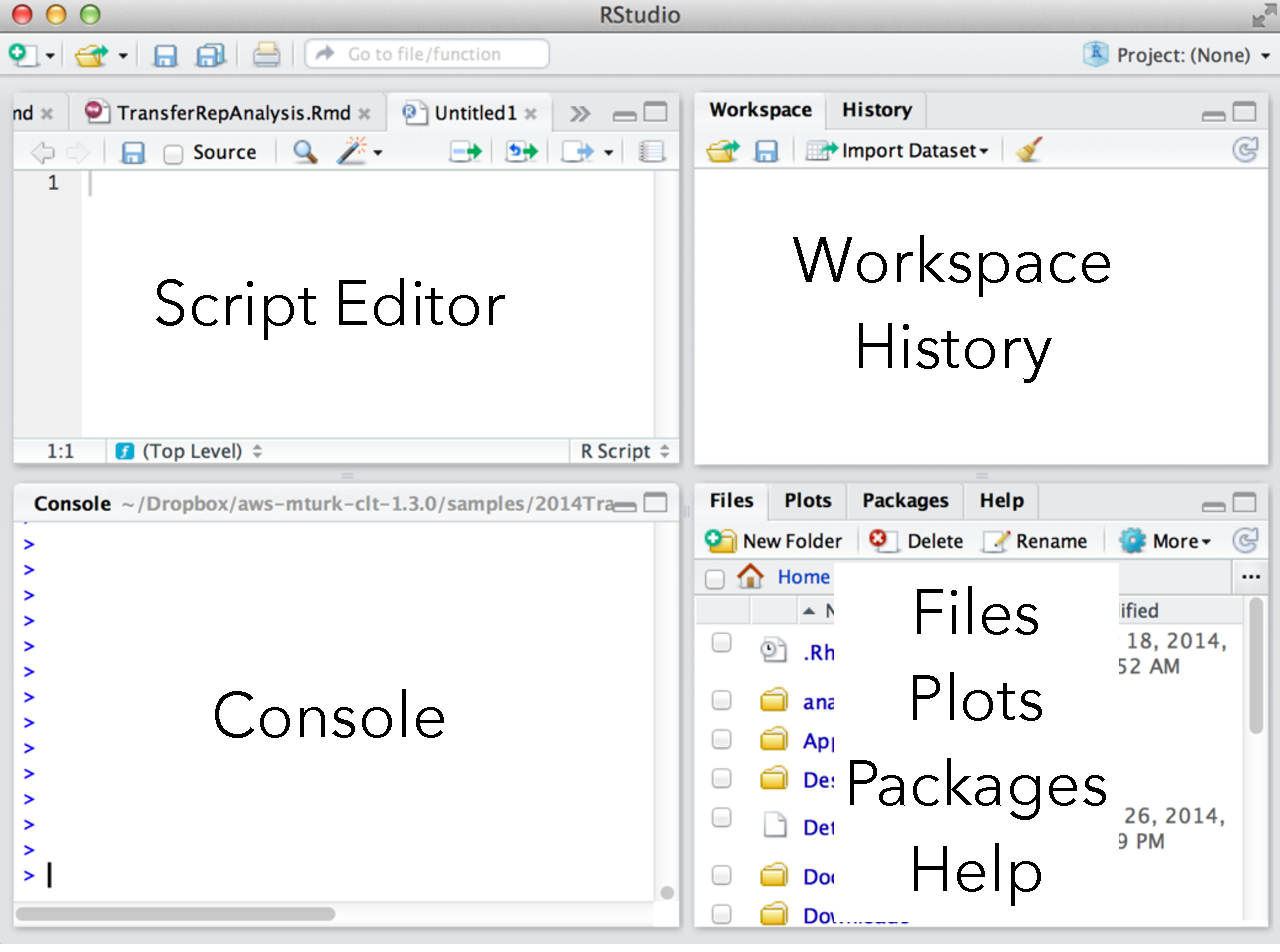
\includegraphics{figures/FigRstudio.pdf}
\caption{\label{fig:2rstudiod}The R-studio workspace}
\end{figure}

\hypertarget{console}{%
\subsubsection{Console}\label{console}}

When you open up R studio you will see three or four main windows (the placement of each are configurable). In the above example, the bottom left window is the command line (terminal or console) for R. This is used to directly enter commands into R. Once you have entered a command here, press enter to execute the command. The console is useful for entering single lines of code and running them. Oftentimes this occurs when you are learning how to correctly execute a line of code in R. Your first few attempts may be incorrect resulting in errors, but trying out different variations on your code in the command line can help you produce the correct code. Pressing the up arrow while in the console will scroll through the most recently executed lines of code.

\hypertarget{script-editor}{%
\subsubsection{Script Editor}\label{script-editor}}

The top left corner contains the script editor. This is a simple text editor for writing and saving R scripts with many lines. Several tabs can be opened at once, with each tab representing a different R script. R scripts can be saved from the editor (resulting in a .r file). Whole scripts can be run by copy and pasting them into the console and pressing enter. Alternatively, you can highlight portions of the script that you want to run (in the script editor) and press command-enter to automatically run that portion in the console (or press the button for running the current line/section: green arrow pointing right).

\hypertarget{workspace-and-history}{%
\subsubsection{Workspace and History}\label{workspace-and-history}}

The top right panel contains two tabs, one for the workspace and another for history. The workspace lists out all of the variables and functions that are currently loaded in R's memory. You can inspect each of the variables by clicking on them. This is generally only useful for variables that do not contain large amounts of information. The history tab provides a record of the recent commands executed in the console.

\hypertarget{file-plot-packages-help}{%
\subsubsection{File, Plot, Packages, Help}\label{file-plot-packages-help}}

The bottom-right window has four tabs for files, plots, packages, and help. The files tab allows browsing of the computers file directory. An important concept in R is the \textbf{current working directory}. This is file folder that R points to by default. Many functions in R will save things directly to this direct, or attempt to read files from this directory. The current working directory can be changed by navigating to the desired folder in the file menu, and then clicking on the more option to set that folder to the current working directory. This is especially important when reading in data to R. The current working directory should be set to the folder containing the data to be inputted into R. The plots tab will show recent plots and figures made in R. The packages tab lists the current R libraries loaded into memory, and provides the ability to download and enable new R packages. The help menu is an invaluable tool. Here, you can search for individual R commands to see examples of how they are used. Sometimes the help files for individual commands are opaque and difficult to understand, so it is necessary to do a Google search to find better examples of using these commands.

\hypertarget{how-to-complete-the-r-labs}{%
\subsection{How to complete the R Labs}\label{how-to-complete-the-r-labs}}

Each of the labs focuses on particular data-analysis problems, from graphing data, computing descriptive statistics, to running inferential tests in R. All of the labs come in three parts, a training part, a generalization part, and a writing part. The training part includes step-by-step examples of R code that solves particular problems. The R code is always highlighted in grey. The generalization part gives short assignments to change parts of the provided code to solve a new problem. The writing part tasks you with answering questions about statitiscal concepts.

The way to complete each lab is to open a new R Markdown document in R-studio, and then document your progression through each of the parts. By doing this, you will become familiar with how R and R-studio works, and how to create documents that preserve both the code and your notes all in one place. There are a few tricks to getting started that are outline below.

\begin{enumerate}
\def\labelenumi{\arabic{enumi}.}
\tightlist
\item
  Open R-studio
\end{enumerate}

\hypertarget{r-projects}{%
\subsubsection{R projects}\label{r-projects}}

\begin{enumerate}
\def\labelenumi{\arabic{enumi}.}
\setcounter{enumi}{1}
\tightlist
\item
  Create a new R project

  \begin{enumerate}
  \def\labelenumii{\alph{enumii}.}
  \tightlist
  \item
    Go to the file menu and select new project, or go to the top right-hand corner of R-studio, you should see a blue cube with an R in it, then select New project from the dropdown menu
  \end{enumerate}
\item
  Save the new R project somewhere that you can find it. If you are working on a lab computer, then save the new R project to the desktop.
\end{enumerate}

What is an R project? When you create a new R project you are creating two things, 1) a new folder on your computer, and 2) a ``.Rproj'' file. For example, if you gave your R project the name ``Lab1'', then you will have created a folder title ``Lab1'', and inside the folder you will find an R project file called ``Lab1.Rproj''.

As you work inside R-studio you will be creating text documents, and you will be doing things like loading data, and saving the results of your analyses. As your work grows and becomes more complex, you can often find yourself creating many different files. \textbf{The R project folder is a very useful way of organizing your files all in one place so you can find them later.} If you double-clik an R project file, R-studio will automatically load and restore your last session. In the labs, you will be using your R project folder to:

\begin{enumerate}
\def\labelenumi{\arabic{enumi}.}
\tightlist
\item
  save data files into this folder
\item
  save R-markdown files that you will use to write your R-code and lab notes
\item
  save the results of your analysis
\end{enumerate}

\hypertarget{installing-libraries}{%
\subsubsection{Installing libraries}\label{installing-libraries}}

When you install R and R-studio, you get what is called Base R. Base R contains many libraries that allow you to conduct statistical anlayses. Because R is free and open-source, many other developers have created add-on libraries that extend the functionality of R. \textbf{We use some of these libraries, and you need to install them before you can do the labs}.

For example, in any of the labs, whenever you see a line code that uses the word library like this \texttt{library(libraryname)}, this line of code telling R to load up that library so it can be used. The \texttt{libraryname} would be replaced with the actual name of the library. For example, you will see code like this in the labs:

\begin{verbatim}
library(data.table)
\end{verbatim}

This line of code is saying that the \texttt{data.table} library needs to be loaded. You can check to see if any library is already loaded by clicking on the ``packages'' tab in the bottom right hand panel. You will see many packages listed in alphabetical order. Packages that are currently loaded and available have a checkmark. If you scroll down and find that you \textbf{do not} have \texttt{data.table} installed, then you need to install it. To install any package follow these steps:

\begin{enumerate}
\def\labelenumi{\arabic{enumi}.}
\tightlist
\item
  Click on the packages tab
\item
  Find the ``install'' button in the top left hand corner of the packages tab.
\item
  Click the install button
\item
  Make sure ``install from:'' is set to CRAN repository
\item
  Make sure ``dependencies'' is clicked on (with a checkmark)
\item
  type the name of the library into the search bar.
\item
  As you type, you should see the names of different packages you can install pop-up in a drop-down menu. \textbf{You must be connected to the internet to install packages from CRAN}
\item
  Once you find the package (e.g., \texttt{data.table}), click it, or just make sure the full, correctly spelled name, is in the search bar
\item
  Press the install button
\end{enumerate}

You should see some text appear in the console while R installs the package.

\begin{enumerate}
\def\labelenumi{\arabic{enumi}.}
\setcounter{enumi}{9}
\tightlist
\item
  After you have installed the package, you should now see that it is listed in the packages tab.
\item
  You can turn the package on by clicking it in the package tab.
\item
  OR, you can turn the packge on by running the command \texttt{library(data.table)} in the console, to do this type \texttt{library(data.table)} into the console, and press enter.
\end{enumerate}

\hypertarget{quick-install}{%
\subsubsection{Quick install}\label{quick-install}}

If you are using R on one of the lab computers, you may find that some of the packages are not installed. The lab computers get wiped everynight, so it may be necessary to install packages each time you come back to the lab. Fortunately, we can tell R to install all of the packages we need in one go. Copy the following lines of code into the console, and press enter. Note you can select all of the lines at once, then copy them, then paste all of them into the console, and press enter to run them all. After each of the packages are installed, you will then be able to load them using \texttt{library()}.

\begin{verbatim}
install.packages(ggplot2)
install.packages(dplyr)
install.packages(data.table)
install.packages(summarytools)
install.packages(gapminder)
install.packages(ggpubr)
\end{verbatim}

\hypertarget{r-markdown}{%
\subsubsection{R markdown}\label{r-markdown}}

Once you have the necessary packages installed you can begin creating R markdown documents for each lab. We admit that at the beginning, R markdown documents might seem a little bit confusing, but you will find they are extremely useful and flexible. Basically, what R markdown allows you to do is combine two kinds of writing, 1) writing R code to conduct analyses, and 2) writing normal text, with headers, sub-headers, and paragraphs. You can think of this like a lab journal, that contains both your writing about what you are doing (e.g., notes to self), and the code that you use for analysis. Additionally, when your code does something like make a graph, or run a statistical test, you can ask R markdown to print the results.

The R markdown website has an excellent tutorial that is well worth your time to check out: \url{https://rmarkdown.rstudio.com/lesson-1.html}

\hypertarget{r-markdown-lab-templates}{%
\subsubsection{R markdown lab templates}\label{r-markdown-lab-templates}}

We have created a set of template documents for each lab that can be downloaded here: \href{https://github.com/CrumpLab/statisticsLab/raw/master/RMarkdownsLab.zip}{download lab templates}.

When you unzip the file you should find the following:

\begin{enumerate}
\def\labelenumi{\arabic{enumi}.}
\tightlist
\item
  A new folder titled ``RMarkdownsLab''
\item
  Inside the folder you will see the ``RMarkdownsLab.Rproj'' file
\item
  A data folder containing data files for the labs
\item
  A ``LabTemplates'' folder containing the R markdown templates for each lab.
\end{enumerate}

To get started with Lab 1, follow these steps:

\begin{enumerate}
\def\labelenumi{\arabic{enumi}.}
\tightlist
\item
  copy the template file for lab 1, ``Lab 01 Graphing\_Student Name.Rmd'', and place it into the ``RMarkdownsLab'' (copy it out of the template folder, and into the RMarkdownsLab folder).
\item
  Rename the file to add your own name, eg., ``Lab1GraphingMattCrump.Rmd''
\item
  double-click the ``RMarkdownsLab.Rproj'' file
\item
  R-studio will now load up.
\item
  If you click the files tab, you will see all of the files and folders inside the ``RMarkdownsLab'' folder
\item
  Click on your lab1 .rmd file, it will now load into the editor window.
\end{enumerate}

Each lab template .rmd file contains three main sections, one for each part of the lab. You will write things inside each section to complete the lab.

\hypertarget{screencast-tutorial}{%
\subsection{Screencast tutorial}\label{screencast-tutorial}}

Follow this guide to get up running for Lab 1.

\hypertarget{r-studio-cloud}{%
\subsection{R-studio Cloud}\label{r-studio-cloud}}

R-studio is also in the cloud. This means that if you want to use R and R-studio through your web-browser you can do that without even installing R or R-studio on your computer. It's also free!

\begin{enumerate}
\def\labelenumi{\arabic{enumi}.}
\item
  sign up for an R-studio cloud account here: \url{https://rstudio.cloud}
\item
  You can make new R projects, work inside them, and everything is saved in the cloud!
\item
  To see how everything would work, follow the steps in this video. You will need to download this \href{https://github.com/CrumpLab/statisticsLab/raw/master/RstudioCloud.zip}{.zip file to your computer to get started}
\end{enumerate}

The link to the video is \url{https://www.youtube.com/watch?v=WsbnV0t7FE4}, or you can watch it here:

\hypertarget{excel}{%
\section{Excel}\label{excel}}

\hypertarget{spss}{%
\section{SPSS}\label{spss}}

\hypertarget{jamovi}{%
\section{JAMOVI}\label{jamovi}}

\hypertarget{cogstat}{%
\section{CogStat}\label{cogstat}}

(using CogStat 2.5rc)

\hypertarget{software-1}{%
\subsection{Software}\label{software-1}}

\hypertarget{introduction}{%
\subsubsection{Introduction}\label{introduction}}

The purpose of this manual is to provide an easy and student-friendly guide for those who would like to learn the basics of statistics using CogStat. This manual is a supplement to Matthew J. C. Crump's book ``Answering Questions With Data - Introductory Statistics For Psychology Students'' and an adaptation of his ``Statistics Lab Manual'' (Answering questions with data: Lab Manual). Through eleven chapters, we will ask questions about data and answer them after running the corresponding analysis. Hopefully, after reading this manual and completing the exercises, you will gain a common understanding of how CogStat can help you with your work. On the other hand, it is important to note that this manual does not have any aspirations for extensive detailing in statistics or CogStat. We will show and explain different matters in CogStat that are useful in practice and real-life but will not reflect on all the underlying theoretical arguments.

\hypertarget{automatic-data-analysis}{%
\subsubsection{Automatic Data Analysis}\label{automatic-data-analysis}}

In automatic data analysis, users do not have to choose individually which analysis to run; instead, they have to choose a question that they would like to answer. It is a powerful method for researchers and students, which is employed partially by many software, but CogStat relies on this method fully, when analyzing data. It helps to reduce human error, which could happen during the analysis or at the interpretation of the results. It is also a partial solution for the replication crisis. The replication crisis refers to the general issue where scientific results are often impossible to replicate. The replicability of research settings and outcomes is a requirement in science that cannot be simply missed. During the early years of the replication crisis, the existence of many previously described phenomena has been questioned due to this problem. Automatic data analysis can help with some of the issues mentioned above. (for more, see: \url{https://en.wikipedia.org/wiki/Replication_crisis\#Background})

Many advantages in line with automatic data analysis can help to moderate the replication crisis and its negative effects. With automatic data analysis, users do not have to choose between loads of settings to run their test correctly. This spares a lot of time and leaves fewer opportunities for mistakes. There is also no need to test assumptions by the user manually since the program does it automatically and chooses the optimal test accordingly. This function is highly favourable, as it relies less on subjectivity; thus, two separate tests-results by two individuals will be identical. With this, the replicability of results could increase. There are some methods where the results highly depend on the chosen analysis because of the absence of consensus in many statistical procedures. This also affects the replicability negatively and might result in incorrect or misleading interpretations. Additionally, note that there are some cases when more analysis methods could be correct for an exact task, this might also cause some difficulty, as well as increase the subjectivity. Automatic data analysis employs a consensual pipeline based on the methodology literature, this reduces the freedom and subjectivity of the researcher and generates greater consensus. It is highly beneficial since mistakes stemming from, for example, lack of statistical knowledge or incorrect knowledge, performance errors, and P-hacking can be eliminated or at least decreased.

\hypertarget{cogstat-1}{%
\subsubsection{CogStat}\label{cogstat-1}}

CogStat is a statistical software that works with automatic data analysis and has an output designed to show the results in a dense, easily interpretable, and informative way (Krajcsi, 2021). CogStat employs the most common tests used in cognitive science research and makes them automated. This means that users cannot choose a single hypothesis test to run; instead, a more general question can be chosen, such as comparing groups. When running the analysis automatically in CogStat, we must provide the data with the appropriate measurement levels for the variables. Setting the right measurement levels is especially important in this method since the software relies heavily on the variable levels when choosing the right analysis to run. Measurement levels must be set before loading the data into CogStat since the software is not designed for editing data. Spreadsheets or statistical software can be used to set the required measurement levels. We also choose what variables we want to run the analysis on, depending on the relations and questions we would like to explore. After that, the software automatically checks the assumptions, runs the corresponding test, and provides an informative output with the data graphed and the most important descriptives and frequency traits without the user's any other interference. This helps to understand the data and statistics more without the need to spend a lot of time untangling the technical details. The previously described optimised output is one of CogStat's most important features. It shows the results in easy-to-understand divisions and also reports them in the current APA style. This makes reporting results faster and more precise, as it can be simply copied and pasted. The output is also well-structured as it is divided into three main parts (Raw data, Sample Properties, and Population Properties) in most cases.

\hypertarget{how-to-start-with-cogstat}{%
\subsubsection{How to start with CogStat}\label{how-to-start-with-cogstat}}

\hypertarget{downloading-and-installing-the-software}{%
\paragraph{Downloading and installing the software}\label{downloading-and-installing-the-software}}

The software is free to download from the official CogStat webpage (\url{https://www.cogstat.org/}) and runs on Windows, Mac, and Linux. (For more and help at the download and installation: \url{https://doc.cogstat.org/Installation})

\hypertarget{data-1}{%
\paragraph{Data}\label{data-1}}

There are many datasets used in this manual, and the majority of it is real data from the original manual by Matthew J. C. Crump (\url{https://github.com/CrumpLab/statistics/tree/master/data}), while others are generated with spreadsheet software. All the datasets that will be used in this manual are available in the CogSat package in the form of demo files. (Data used in this manual can be found in the folder ``Haasz. Answering questions with data Lab Manual''.) These types of datasets can be loaded from there, in the following ways shown in the pictures below.

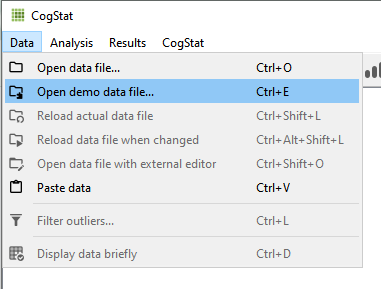
\includegraphics{img/intro/opendemodata_menu.png}

or

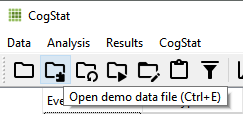
\includegraphics{img/intro/opendemodata_icon.png}

After choosing the option ``Data'' and ``Open demo data file'' you can reach any demo data from the CogStat package. With ``Open data file'', you can use any other dataset you have on your computer that is in the right format that CogStat can handle. You can also load data from different programs with the copy-paste function, using the clipboard. Simply select and copy the data you would like to use and paste it into the CogStat window. It can be especially important when you do not want to use the whole dataset for the analysis, so only some parts will be copied and pasted. Also, to open a file, you can drag and drop it into the CogStat window, too.

\hypertarget{setting-the-measurement-levels}{%
\paragraph{Setting the measurement levels}\label{setting-the-measurement-levels}}

CogStat cannot be used for editing your data, meaning you have to use a spreadsheet or another statistical software to store and edit it. (It is another reason why the copy-and-paste function is helpful.) Before loading your data into CogStat, it is advised to check it and set all the measurement levels for all variables. Many file format is supported (e.g., Excel spreadsheet, OpenDocument spreadsheet, Text files, SPSS, Japs, Jamovi files, and others\ldots{} ) (for more: \url{https://doc.cogstat.org/Handling-data}) (If you use the demo datafiles that belong to this manual, you will see that we set the measurement levels for you.)

There are two methods to set measurement levels in the dataset. If the data is stored in a spreadsheet format (e.g.~Microsoft Excel, Google Spreadsheet, etc.), a second row should be added, including int, ord, and nom for the interval, ordinal, and nominal measurement levels (second row, after the variable names). Note that ratio variables are also handled as intervals, and string variables will be set to nominal automatically.

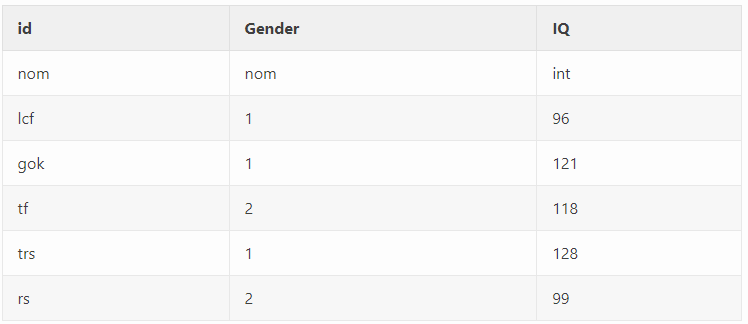
\includegraphics{img/intro/measurementlevels.png}

Another way to set the measurement level is to use other statistical software, where you can adjust them, and after saving the data, you can open it with CogStat. For example, in SPSS, you can set the measurement levels and then open the file into the CogStat window. However, be aware that the measurement levels cannot be set in every statistical software, so in this case, information about measurement levels will be missing when importing your data from such a source (e.g.~R files or STATA files). If measurement levels for the dataset are not set before loading it into CogStat, CogStat will set it to unknown (unk) and, in most cases, will handle it as interval variables. Analysis can be run like this, but if it is not your intention to have your data handled as interval variables, then set the right measurement levels.
For more on handling data: \url{https://doc.cogstat.org/Handling-data}.

If you need additional information or would like to learn more about CogStat, there are many sources:

\begin{itemize}
\item
  A brief description of how to start using the software (\url{https://doc.cogstat.org/Quick-Start-Tutorial})
\item
  The user documentation of the software (\url{https://doc.cogstat.org/})
\item
  Advantages of using CogStat (\url{https://docs.google.com/presentation/d/1dIb6f3yPvr8stMLS7b7qcBsgloqbcQj2b55NUT4D9vc/edit\#slide=id.p})
\item
  Using CogStat for your analysis (\url{https://docs.google.com/presentation/d/1_rnHhyD3pF9BZuqCkcFLWKhAbX1DfS8T5q-TxogqpZA/edit\#slide=id.p})
\end{itemize}

\hypertarget{navigating-in-the-manual}{%
\subsection{Navigating in the manual}\label{navigating-in-the-manual}}

From the next section of this Manual, you will solve specific problems through eleven chapters with the help of CogStat. There are some CogStat features that, despite being fundamental and useful, only appear in later chapters. It is because we tried to follow the order of the other software guides employed in the manual, for transparency. On the other hand, automatic data analysis and CogStat have a unique philosophy which is often not in line with the manual data analysis point of view. This elemental difference in methodology might also contribute to some parts being located unnaturally. To help with finding the personally relevant parts for everyone, we named the chapters and subchapters carefully, so they cover their most important contents properly. It is advised to navigate in the table of contents if there is a specific feature of CogStat you need to find.

There are many additional features and analyses to CogStat that are not included in this manual but are worth mentioning, for example, regressions, power analysis, reliability analysis (internal consistency reliability analysis and interrater reliability analysis) and (behavioural data) diffusion analysis. Results of Bayesian hypothesis tests are also provided in most cases and pivot tables can be created\ldots{} Some other important features that are not mentioned in the following chapters are that in almost every dialogue a help button is provided with useful instructions. Another important feature is that spreadsheet software can be used as data view. This means that with every saved change in your spreadsheet, data also changes in CogStat and the analysis can be rerunned. These settings are not automatic, they must be set.

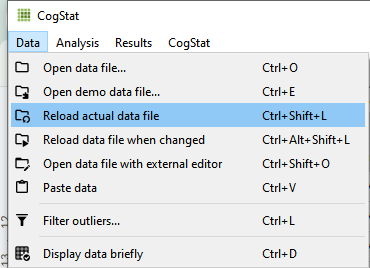
\includegraphics{img/intro/reloadfile_menu.png}

or


\includegraphics{img/intro/reload_icon.png}

With ``Reload the actual data file'', the data that has been changed and saved in the spreadsheet software will also change in CogStat. With ``Reload data file when changed'', the previous analysis will be rerunned with the changes made.

\hypertarget{lab-1-graphing-data}{%
\chapter{Lab 1: Graphing Data}\label{lab-1-graphing-data}}

{
The commonality between science and art is in trying to see profoundly - to develop strategies of seeing and showing.
---Edward Tufte
}

As we have found out from the textbook and lecture, when we measure things, we get lots of numbers. Too many. Sometimes so many your head explodes just thinking about them. One of \textbf{the most helpful things} you can do to begin to make sense of these numbers, is to look at them in graphical form. Unfortunately, for sight-impaired individuals, graphical summary of data is much more well-developed than other forms of summarizing data for our human senses. Some researchers are developing auditory versions of visual graphs, a process called \textbf{sonification}, but we aren't prepared to demonstrate that here. Instead, we will make charts, and plots, and things to look at, rather than the numbers themselves, mainly because these are tools that are easiest to get our hands on, they are the most developed, and they work really well for visual summary. If time permits, at some point I would like to come back here and do the same things with sonification. I think that would be really, really cool!

\hypertarget{general-goals}{%
\section{General Goals}\label{general-goals}}

Our general goals for this first lab are to get your feet wet, so to speak. We'll do these things:

\begin{enumerate}
\def\labelenumi{\arabic{enumi}.}
\tightlist
\item
  Load in some data to a statistical software program
\item
  Talk a little bit about how the data is structured
\item
  Make graphs of the data so we can look at it and make sense of it.
\end{enumerate}

\hypertarget{important-info}{%
\subsection{Important info}\label{important-info}}

\begin{enumerate}
\def\labelenumi{\arabic{enumi}.}
\item
  Data for NYC film permits was obtained from the NYC open data website. The .csv file can be found here: Film\_Permits.csv
\item
  Gapminder data from the gapminder project (copied from the R gapminder library) can be downloaded in .csv format here: gapminder.csv
\end{enumerate}

\hypertarget{r-1}{%
\section{R}\label{r-1}}

\hypertarget{download-the-lab-templates}{%
\subsection{Download the lab templates}\label{download-the-lab-templates}}

You will be completing each lab by writing your code and notes in an R Markdown document.

\begin{enumerate}
\def\labelenumi{\arabic{enumi}.}
\tightlist
\item
  Download the \href{https://github.com/CrumpLab/statisticsLab/raw/master/RMarkdownsLab.zip}{RMarkdownsLab.zip} to your computer.
\item
  Unzip the file, this will produce a new folder with three important parts

  \begin{enumerate}
  \def\labelenumii{\alph{enumii}.}
  \tightlist
  \item
    data folder (contains data files for all labs)
  \item
    LabTemplates folder (contains blank templates for completing all the labs)
  \item
    RMarkdownsLab.Rproj A file with a little blue cube with an R in it.
  \end{enumerate}
\item
  Double-click the RMarkdownsLab.Rproj file, this will automatically open R-studio (if you are at home, you must \href{https://crumplab.github.io/statisticsLab/software.html\#installing-r-and-r-studio}{install R and R-studio first}, or you can use \href{https://crumplab.github.io/statisticsLab/software.html\#r-studio-cloud}{R-studio Cloud} through your web-browser)
\item
  Copy the template .Rmd file for lab 1 from the LabTemplates folder into the main folder, then open it, and use it to begin adding your code and notes for lab 1.
\item
  Watch this screencast to help you get started.
\end{enumerate}

Your lab instructor will show you how to open R-studio on the lab computer. Just find it and double-click. Now you have R-studio. Your lab instructor will also walk you through the steps to get started completing the first lab. We also wrote down the steps \href{https://crumplab.github.io/statisticsLab/software.html\#how-to-complete-the-r-labs}{here}.

There are numerous resources for learning about R, we put some of them on the course website, under the \href{https://crumplab.github.io/psyc3400/Resources.html}{resouces page}. You will find these resources helpful as you learn. We also have a kind of \href{https://crumplab.github.io/statisticsLab/software.html\#r}{general introduction to R and Rstudio here}. This shows you how to download R and R-studio at home (it's free). Throughout the labs you will be writing things called R Markdown documents. You will learn how to do this throughout the labs, but it can also be worthwhile reading other tutorials, such as the one provided by \href{https://rmarkdown.rstudio.com/lesson-1.html}{R Markdown}.

When we made this course, we assumed that most students would be unfamiliar with R and R-studio, and might even be frightened of it, because it is a computer programming language (OOOOHHH NOOOOOOO, I NEED TO DROP THIS COURSE NOW)\ldots Don't worry. It's going to be way easier than you think. Let's compare to other statistics courses where you would learn something like SPSS. That is also a limited programming language, but you would mostly learn how to point with a mouse, and click with button. I bet you already know how to do that. I bet you also already know how to copy and paste text, and press enter. That's mostly what we'll be doing to learn R. We will be doing statistics by typing commands, rather than by clicking buttons. However, lucky for you, all of the commands are already written for you. You just have to copy/paste them.

We know that this will seem challenging at first. But, we think that with lots of working examples, you will get the hang of it, and by the end of the course you will be able to do things you might never have dreamed you can do. It's really a fantastic skill to learn, even if you aren't planning on going on to do research in Psychology (in which case, this kind of thing is necessary skill to learn). With that, let's begin.

\hypertarget{get-some-data}{%
\subsection{Get some data}\label{get-some-data}}

In order to graph data, we need to have some data first\ldots Actually, with R, that's not quite true. Run this bit of code and see what happens:

\begin{Shaded}
\begin{Highlighting}[]
\FunctionTok{hist}\NormalTok{(}\FunctionTok{rnorm}\NormalTok{(}\DecValTok{100}\NormalTok{, }\AttributeTok{mean=}\DecValTok{50}\NormalTok{, }\AttributeTok{sd=}\DecValTok{25}\NormalTok{))}
\end{Highlighting}
\end{Shaded}

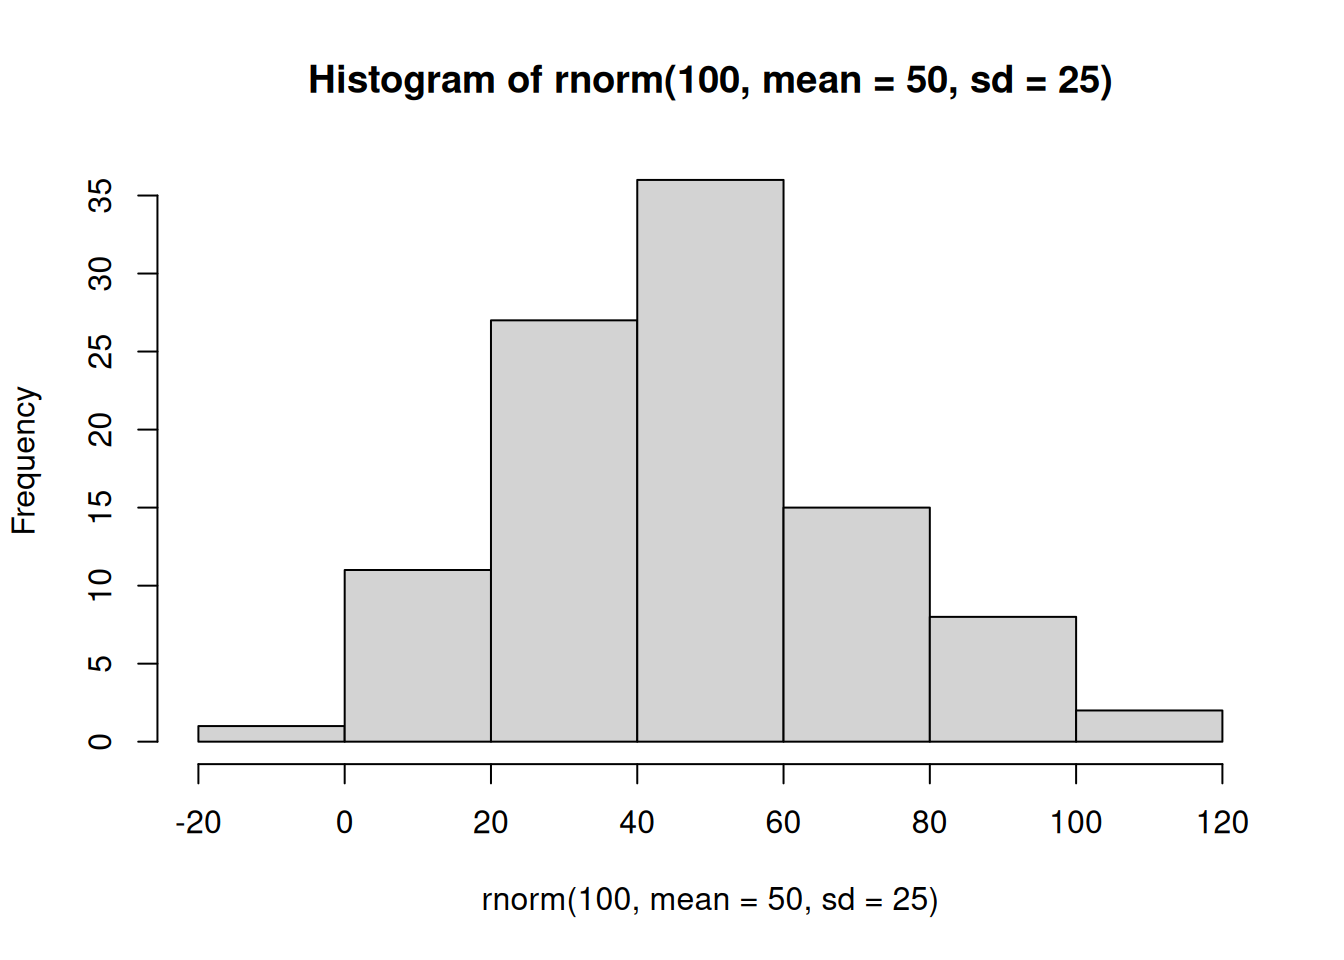
\includegraphics{Statistics_Lab_files/figure-latex/unnamed-chunk-7-1.pdf}

You just made R sample 100 numbers, and then plot the results in a histogram. Pretty neat. We'll be doing some of this later in the course, where get R to make fake data for us, and then we learn to think about how data behaves under different kinds of assumptions.

For now, let's do something that might be a little bit more interesting\ldots what movies are going to be filming in NYC? It turns out that NYC makes a lot of data about a lot things open and free for anyone to download and look at. This is the NYC Open Data website: \url{https://opendata.cityofnewyork.us}. I searched through the data, and found a data file that lists the locations of film permits for shooting movies all throughout the Burroughs. There are multiple ways to load this data into R.

\begin{enumerate}
\def\labelenumi{\arabic{enumi}.}
\tightlist
\item
  If you have downloaded the \href{https://github.com/CrumpLab/statisticsLab/raw/master/RMarkdownsLab.zip}{RMarkdownsLab.zip} file, then you already have the data file in the data folder. Assuming you are working in your main directory (your .rmd file is saved in the main folder that contains both the data and template folders), then use the following commands to load the data.
\end{enumerate}

\begin{Shaded}
\begin{Highlighting}[]
\FunctionTok{library}\NormalTok{(data.table)}
\NormalTok{nyc\_films }\OtherTok{\textless{}{-}}\FunctionTok{fread}\NormalTok{(}\StringTok{"data/Film\_Permits.csv"}\NormalTok{)}
\end{Highlighting}
\end{Shaded}

\begin{enumerate}
\def\labelenumi{\arabic{enumi}.}
\setcounter{enumi}{1}
\tightlist
\item
  If the above method doesn't work, you can try loading the data from the course website using:
\end{enumerate}

\begin{Shaded}
\begin{Highlighting}[]
\FunctionTok{library}\NormalTok{(data.table)}
\NormalTok{nyc\_films }\OtherTok{\textless{}{-}} \FunctionTok{fread}\NormalTok{(}\StringTok{"https://raw.githubusercontent.com/CrumpLab/statisticsLab/master/data/Film\_Permits.csv"}\NormalTok{)}
\end{Highlighting}
\end{Shaded}

If you are having issues getting the data loaded, then talk to your lab instructor

\hypertarget{look-at-the-data}{%
\subsection{Look at the data}\label{look-at-the-data}}

You will be downloading and analyzing all kinds of data files this semester. We will follow the very same steps every time. The steps are to load the data, then look at it. You want to see what you've got.

In R-studio, you will now see a variable called \texttt{nyc\_films} in the top right-hand corner of the screen, in the environment tab. If you click this thing, it will show you the contents of the data in a new window. The data is stored in something we call a \texttt{data\ frame}. It's R lingo, for the thing that contains the data. Notice is a square, with rows going across, and columns going up and down. It looks kind of like an excel spreadsheet if you are familiar with Excel.

It's useful to know you can look at the data frame this way if you need to. But, this data frame is really big, it has 50,728 rows of data. That's a lot too much to look at.

\hypertarget{summarytools}{%
\subsubsection{summarytools}\label{summarytools}}

The summarytools packages give a quick way to summarize all of the data in a data frame. Here's how. When you run this code you will see the summary in the viewer on the bottom right hand side. There's a little browser button (arrow on top of little window) that you can click to expand and see the whole thing in a browser.

\begin{Shaded}
\begin{Highlighting}[]
\FunctionTok{library}\NormalTok{(summarytools)}
\FunctionTok{view}\NormalTok{(}\FunctionTok{dfSummary}\NormalTok{(nyc\_films))}
\end{Highlighting}
\end{Shaded}

That is super helpful, but it's still a lot to look at. Because there is so much data here, it's pretty much mind-boggling to start thinking about what to do with it.

\hypertarget{make-plots-to-answer-questions}{%
\subsection{Make Plots to answer questions}\label{make-plots-to-answer-questions}}

Let's walk through a couple questions we might have about this data. We can see that there were 50,728 film permits made. We can also see that there are different columns telling us information about each of the film permits. For example, the \texttt{Borough} column lists the Borough for each request, whether it was made for: Manhattan, Brooklyn, Bronx, Queen's, or Staten Island. Now we can ask our first question, and learn how to do some plotting in R.

\hypertarget{where-are-the-most-film-permits-being-requested}{%
\subsubsection{Where are the most film permits being requested?}\label{where-are-the-most-film-permits-being-requested}}

Do you have any guesses? Is it Manhattan, or Brooklyn, of the Bronx? Or Queen's or Staten Island? We can find out by plotting the data using a bar plot. We just need to count how many film permits are made in each borough, and then make different bars represent the the counts.

First, we do the counting in R. Run the following code.

\begin{Shaded}
\begin{Highlighting}[]
\FunctionTok{library}\NormalTok{(dplyr)}

\NormalTok{counts }\OtherTok{\textless{}{-}}\NormalTok{ nyc\_films }\SpecialCharTok{\%\textgreater{}\%}
          \FunctionTok{group\_by}\NormalTok{(Borough) }\SpecialCharTok{\%\textgreater{}\%}
          \FunctionTok{summarize}\NormalTok{(}\AttributeTok{count\_of\_permits =} \FunctionTok{length}\NormalTok{(Borough))}
\end{Highlighting}
\end{Shaded}

The above grouped the data by each of the five Borough's, and then counted the number of times each Borough occurred (using the \texttt{length} function). The result is a new variable called \texttt{count}. I chose to name this variable \texttt{count}. You can see that it is now displayed in the top-right hand corned in the environment tab. If you gave \texttt{count} a different name, like \texttt{muppets}, then it would be named what you called it.

If you click on the \texttt{counts} variable, you will see the five boroughs listed, along with the counts for how many film permits were requested in each Borough. These are the numbers that we want to plot in a graph.

We do the plot using a fantastic package called \texttt{ggplot2}. It is very powerful once you get the hand of it, and when you do, you will be able to make all sorts of interesting graphs. Here's the code to make the plot

\begin{Shaded}
\begin{Highlighting}[]
\FunctionTok{library}\NormalTok{(ggplot2)}

\FunctionTok{ggplot}\NormalTok{(counts, }\FunctionTok{aes}\NormalTok{(}\AttributeTok{x =}\NormalTok{ Borough, }\AttributeTok{y =}\NormalTok{ count\_of\_permits )) }\SpecialCharTok{+}
  \FunctionTok{geom\_bar}\NormalTok{(}\AttributeTok{stat=}\StringTok{"identity"}\NormalTok{)}
\end{Highlighting}
\end{Shaded}

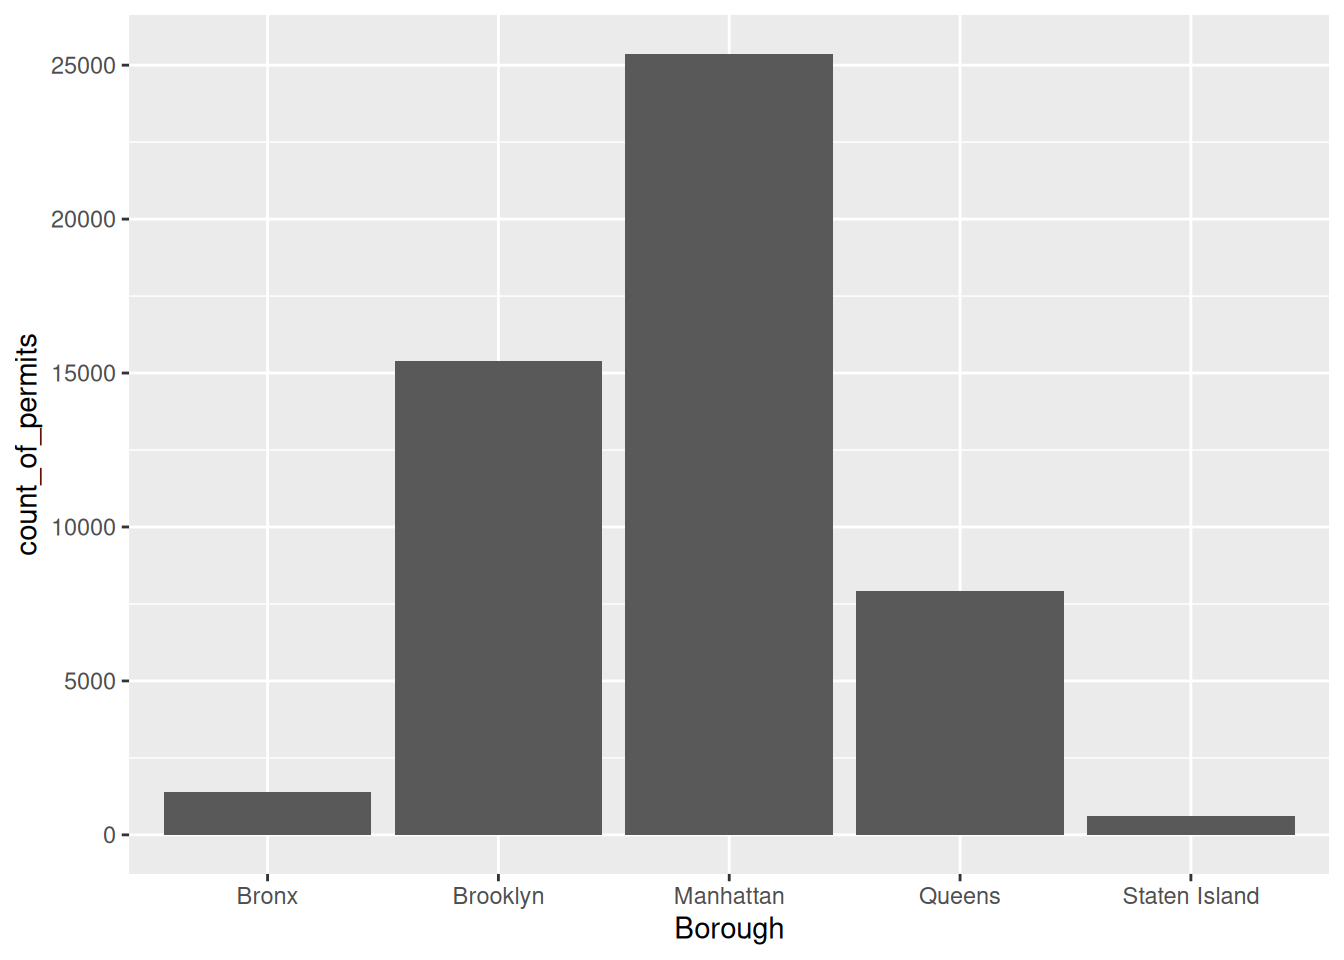
\includegraphics{Statistics_Lab_files/figure-latex/1borough-1.pdf}

There it is, we're done here! We can easily look at this graph, and answer our question. Most of the film permits were requested in Manhattan, followed by Brooklyn, then Queen's, the Bronx, and finally Staten Island.

\hypertarget{what-kind-of-films-are-being-made-what-is-the-category}{%
\subsubsection{What kind of ``films'' are being made, what is the category?}\label{what-kind-of-films-are-being-made-what-is-the-category}}

We think you might be skeptical of what you are doing here, copying and pasting things. Soon you'll see just how fast you can do things by copying and pasting, and make a few little changes. Let's quickly ask another question about what kinds of films are being made. The column \texttt{Category}, gives us some information about that. Let's just copy paste the code we already made, and see what kinds of categories the films fall into. See if you can tell what I changed in the code to make this work, I'll do it all at once:

\begin{Shaded}
\begin{Highlighting}[]
\NormalTok{counts }\OtherTok{\textless{}{-}}\NormalTok{ nyc\_films }\SpecialCharTok{\%\textgreater{}\%}
          \FunctionTok{group\_by}\NormalTok{(Category) }\SpecialCharTok{\%\textgreater{}\%}
          \FunctionTok{summarize}\NormalTok{(}\AttributeTok{count\_of\_permits =} \FunctionTok{length}\NormalTok{(Category))}

\FunctionTok{ggplot}\NormalTok{(counts, }\FunctionTok{aes}\NormalTok{(}\AttributeTok{x =}\NormalTok{ Category, }\AttributeTok{y =}\NormalTok{ count\_of\_permits )) }\SpecialCharTok{+}
  \FunctionTok{geom\_bar}\NormalTok{(}\AttributeTok{stat=}\StringTok{"identity"}\NormalTok{)}\SpecialCharTok{+} 
  \FunctionTok{theme}\NormalTok{(}\AttributeTok{axis.text.x =} \FunctionTok{element\_text}\NormalTok{(}\AttributeTok{angle =} \DecValTok{90}\NormalTok{, }\AttributeTok{hjust =} \DecValTok{1}\NormalTok{))}
\end{Highlighting}
\end{Shaded}

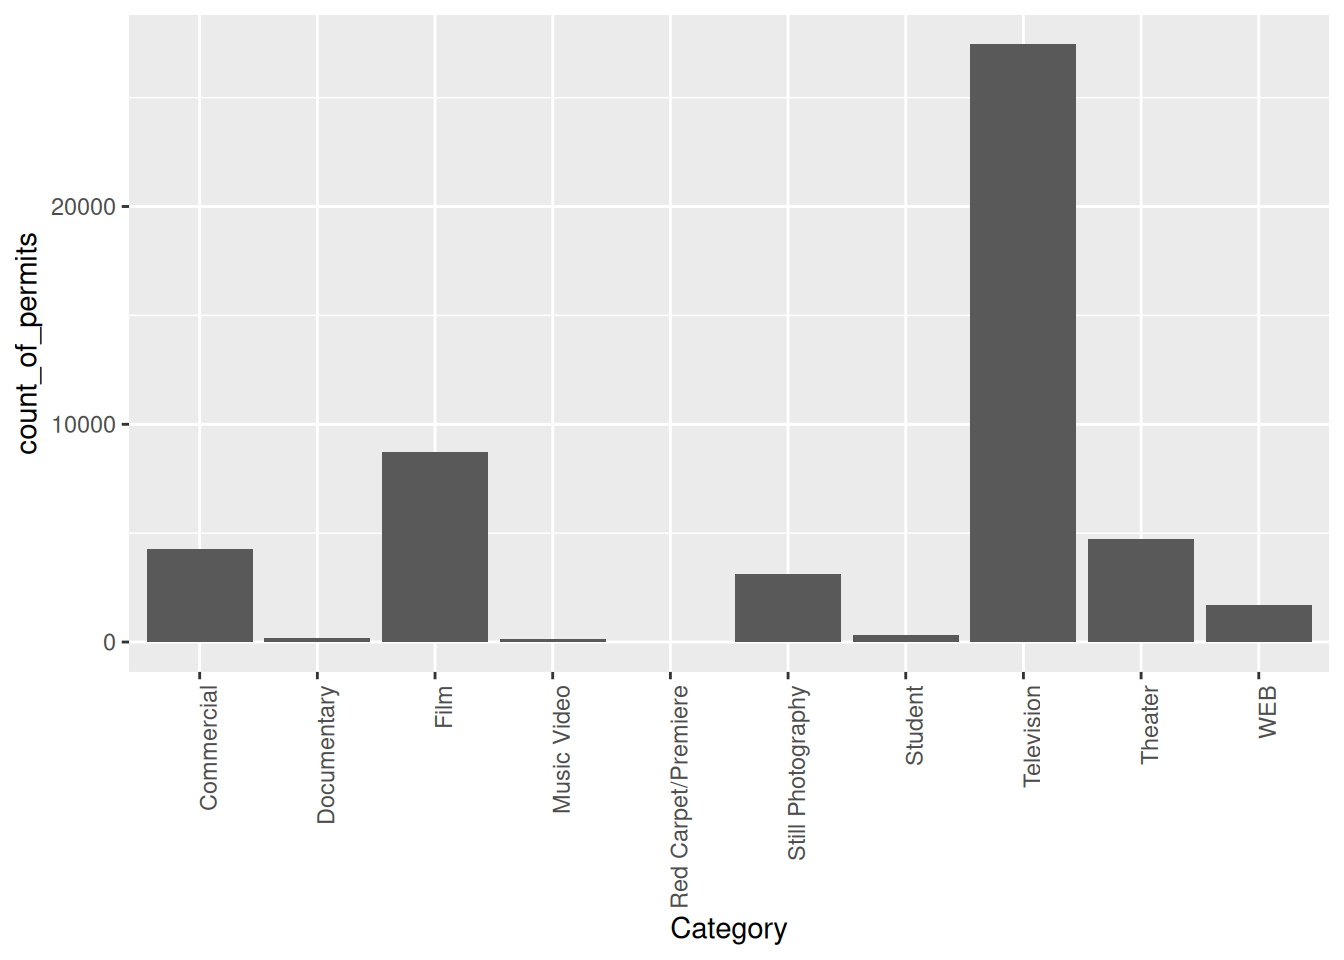
\includegraphics{Statistics_Lab_files/figure-latex/1category-1.pdf}

OK, so this figure might look a bit weird because the labels on the bottom are running into each other. We'll fix that in a bit. First, let's notice the changes.

\begin{enumerate}
\def\labelenumi{\arabic{enumi}.}
\item
  I changed \texttt{Borough} to \texttt{Category}. That was the main thing
\item
  I left out a bunch of things from before. None of the \texttt{library()} commands are used again, and I didn't re-run the very early code to get the data. R already has those things in it's memory, so we don't need to do that first. If you ever clear the memory of R, then you will need to reload those things. First-things come first.
\end{enumerate}

Fine, so how do we fix the graph? Good question. To be honest, I don't know right now. I totally forgot how. But, I know ggplot2 can do this, and I'm going to Google it, right now. Then I'm going to find the answer, and use it here. The googling of your questions is a fine way to learn. It's what everybody does these days\ldots.{[}goes to Google\ldots{]}.

Found it, actually found a lot of ways to do this. The trick is to add the last line. I just copy-pasted it from the solution I found on \href{https://stackoverflow.com/questions/1330989/rotating-and-spacing-axis-labels-in-ggplot2}{stack overflow} (you will become friend's with stack overflow, there are many solutions there to all of your questions)

\begin{Shaded}
\begin{Highlighting}[]
\NormalTok{counts }\OtherTok{\textless{}{-}}\NormalTok{ nyc\_films }\SpecialCharTok{\%\textgreater{}\%}
          \FunctionTok{group\_by}\NormalTok{(Category) }\SpecialCharTok{\%\textgreater{}\%}
          \FunctionTok{summarize}\NormalTok{(}\AttributeTok{count\_of\_permits =} \FunctionTok{length}\NormalTok{(Category))}

\FunctionTok{ggplot}\NormalTok{(counts, }\FunctionTok{aes}\NormalTok{(}\AttributeTok{x =}\NormalTok{ Category, }\AttributeTok{y =}\NormalTok{ count\_of\_permits )) }\SpecialCharTok{+}
  \FunctionTok{geom\_bar}\NormalTok{(}\AttributeTok{stat=}\StringTok{"identity"}\NormalTok{)}\SpecialCharTok{+} 
  \FunctionTok{theme}\NormalTok{(}\AttributeTok{axis.text.x =} \FunctionTok{element\_text}\NormalTok{(}\AttributeTok{angle =} \DecValTok{90}\NormalTok{, }\AttributeTok{hjust =} \DecValTok{1}\NormalTok{))}
\end{Highlighting}
\end{Shaded}

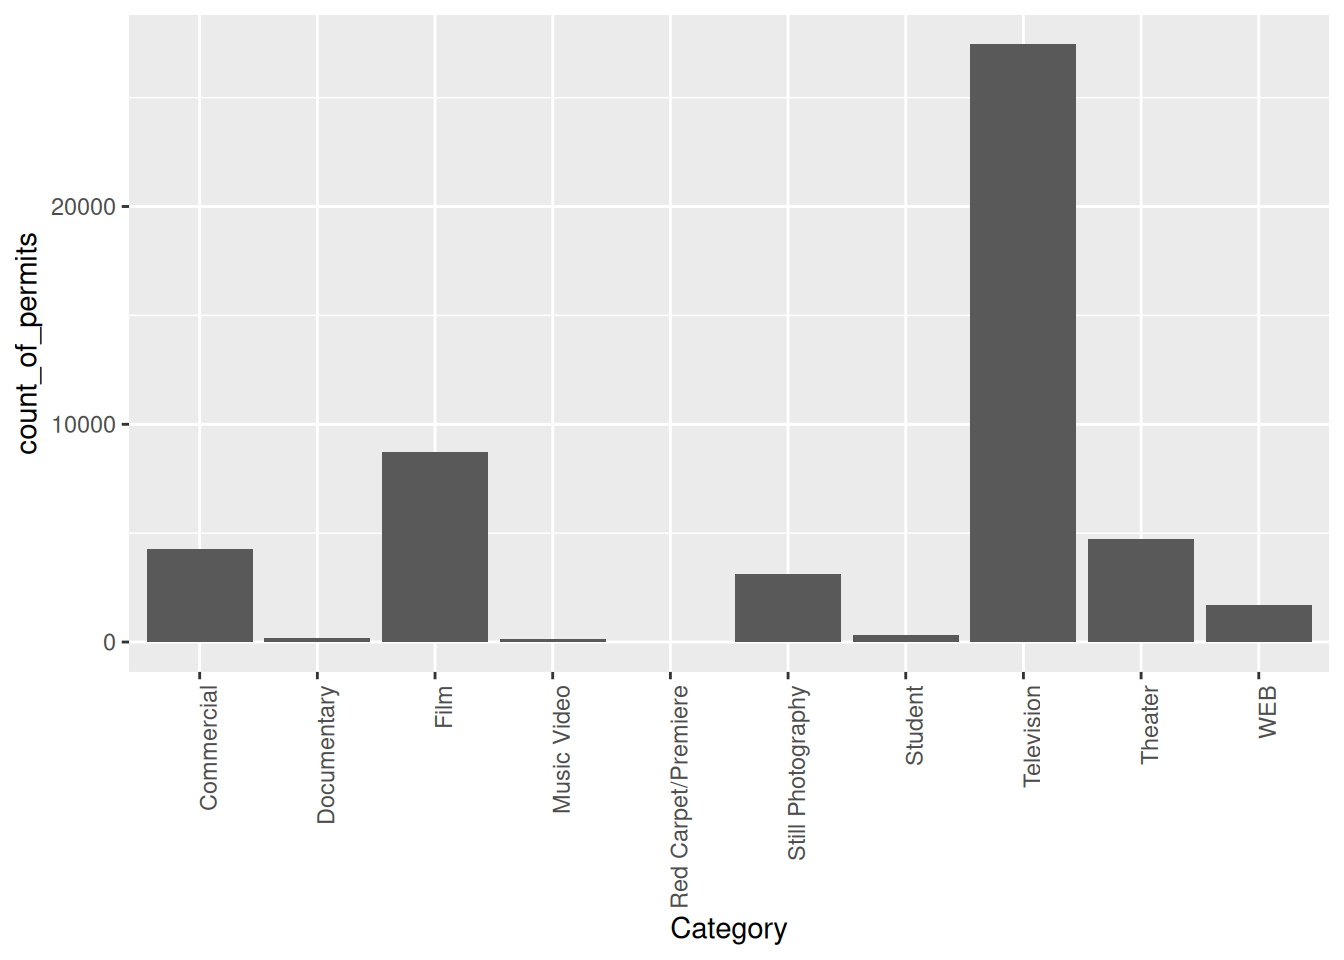
\includegraphics{Statistics_Lab_files/figure-latex/1categoryB-1.pdf}

\hypertarget{ggplot2-basics}{%
\subsection{ggplot2 basics}\label{ggplot2-basics}}

Before we go further, I want to point out some basic properties of ggplot2, just to give you a sense of how it is working. This will make more sense in a few weeks, so come back here to remind yourself. We'll do just a bit a basics, and then move on to making more graphs, by copying and pasting.

The ggplot function uses layers. Layers you say? What are these layers? Well, it draws things from the bottom up. It lays down one layer of graphics, then you can keep adding on top, drawing more things. So the idea is something like: Layer 1 + Layer 2 + Layer 3, and so on. If you want Layer 3 to be Layer 2, then you just switch them in the code.

Here is a way of thinking about ggplot code

\begin{verbatim}
ggplot(name_of_data, aes(x = name_of_x_variable, y = name_of_y_variable)) +
    geom_layer()+
    geom_layer()+
    geom_layer()
\end{verbatim}

What I want you to focus on in the above description is the \(+\) signs. What we are doing with the plus signs is adding layers to plot. The layers get added in the order that they are written. If you look back to our previous code, you will see we add a \texttt{geom\_bar} layer, then we added another layer to change the rotation of the words on the x-axis. This is how it works.

BUT WAIT? How am I supposed to know what to add? This is nuts! We know. You're not supposed to know just yet, how could you? We'll give you lots of examples where you can copy and paste, and they will work. That's how you'll learn. If you really want to read the \href{https://ggplot2.tidyverse.org/reference/index.html}{help manual} you can do that too. It's on the ggplot2 website. This will become useful after you already know what you are doing, before that, it will probably just seem very confusing. However, it is pretty neat to look and \href{http://www.ggplot2-exts.org/gallery/}{see all of the different things you can do}, it's very powerful.

For now, let's the get the hang of adding things to the graph that let us change some stuff we might want to change. For example, how do you add a title? Or change the labels on the axes? Or add different colors, or change the font-size, or change the background? You can change all of these things by adding different lines to the existing code.

\hypertarget{ylab-changes-y-label}{%
\subsubsection{ylab() changes y label}\label{ylab-changes-y-label}}

The last graph had \texttt{count\_of\_permits} as the label on the y-axis. That doesn't look right. ggplot2 automatically took the label from the column, and made it be the name on the y-axis. We can change that by adding \texttt{ylab("what\ we\ want")}. We do this by adding a \(+\) to the last line, then adding \texttt{ylab()}

\begin{Shaded}
\begin{Highlighting}[]
\FunctionTok{ggplot}\NormalTok{(counts, }\FunctionTok{aes}\NormalTok{(}\AttributeTok{x =}\NormalTok{ Category, }\AttributeTok{y =}\NormalTok{ count\_of\_permits )) }\SpecialCharTok{+}
  \FunctionTok{geom\_bar}\NormalTok{(}\AttributeTok{stat=}\StringTok{"identity"}\NormalTok{) }\SpecialCharTok{+} 
  \FunctionTok{theme}\NormalTok{(}\AttributeTok{axis.text.x =} \FunctionTok{element\_text}\NormalTok{(}\AttributeTok{angle =} \DecValTok{90}\NormalTok{, }\AttributeTok{hjust =} \DecValTok{1}\NormalTok{)) }\SpecialCharTok{+}
  \FunctionTok{ylab}\NormalTok{(}\StringTok{"Number of Film Permits"}\NormalTok{)}
\end{Highlighting}
\end{Shaded}

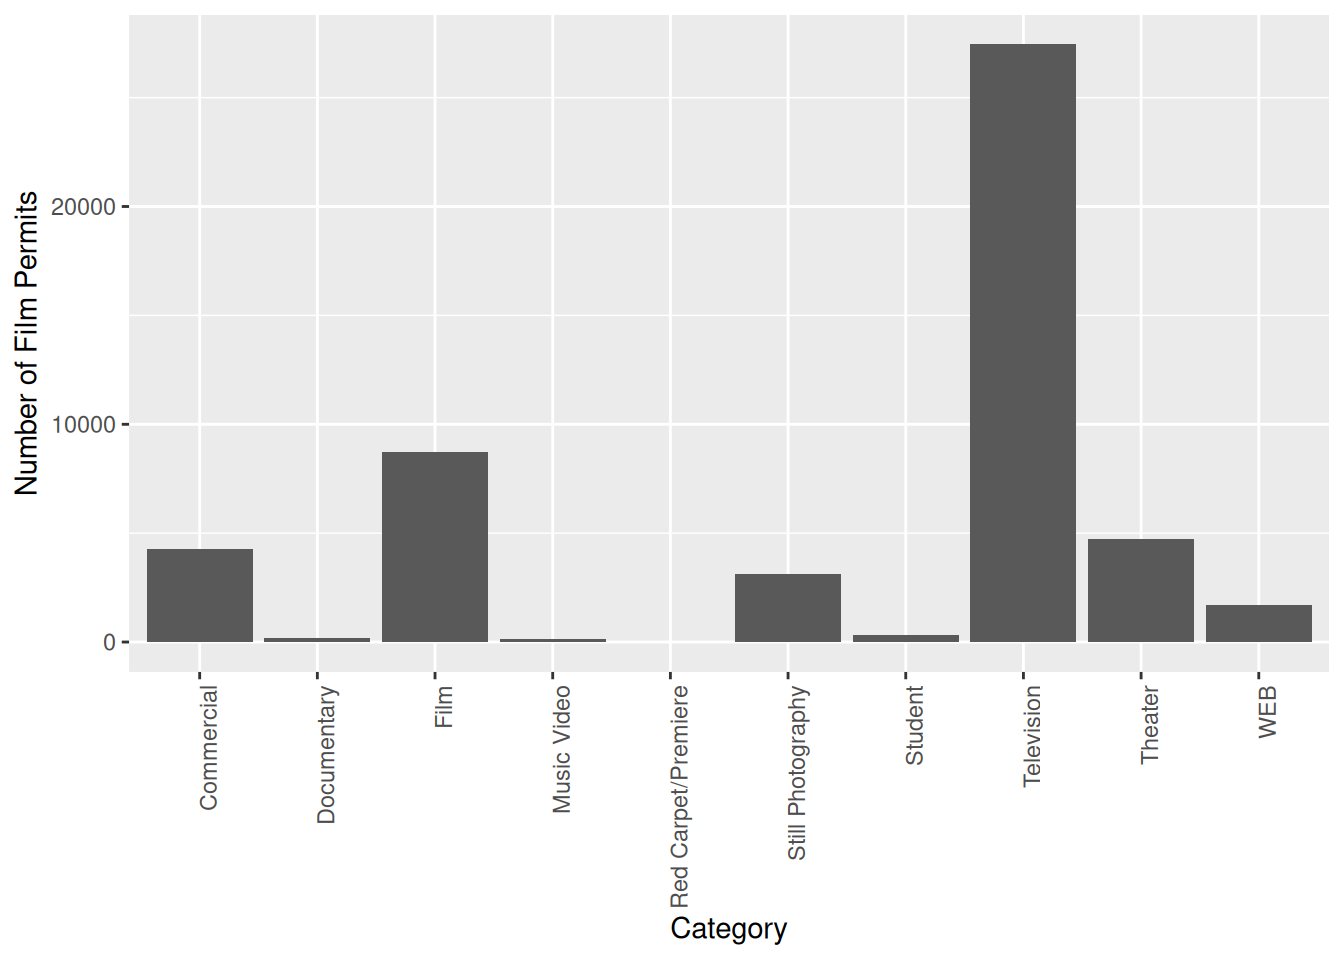
\includegraphics{Statistics_Lab_files/figure-latex/1categoryC-1.pdf}

\hypertarget{xlab-changes-x-label}{%
\subsubsection{xlab() changes x label}\label{xlab-changes-x-label}}

Let's slightly modify the x label too:

\begin{Shaded}
\begin{Highlighting}[]
\FunctionTok{ggplot}\NormalTok{(counts, }\FunctionTok{aes}\NormalTok{(}\AttributeTok{x =}\NormalTok{ Category, }\AttributeTok{y =}\NormalTok{ count\_of\_permits )) }\SpecialCharTok{+}
  \FunctionTok{geom\_bar}\NormalTok{(}\AttributeTok{stat=}\StringTok{"identity"}\NormalTok{) }\SpecialCharTok{+} 
  \FunctionTok{theme}\NormalTok{(}\AttributeTok{axis.text.x =} \FunctionTok{element\_text}\NormalTok{(}\AttributeTok{angle =} \DecValTok{90}\NormalTok{, }\AttributeTok{hjust =} \DecValTok{1}\NormalTok{)) }\SpecialCharTok{+}
  \FunctionTok{ylab}\NormalTok{(}\StringTok{"Number of Film Permits"}\NormalTok{) }\SpecialCharTok{+} 
  \FunctionTok{xlab}\NormalTok{(}\StringTok{"Category of film"}\NormalTok{)}
\end{Highlighting}
\end{Shaded}

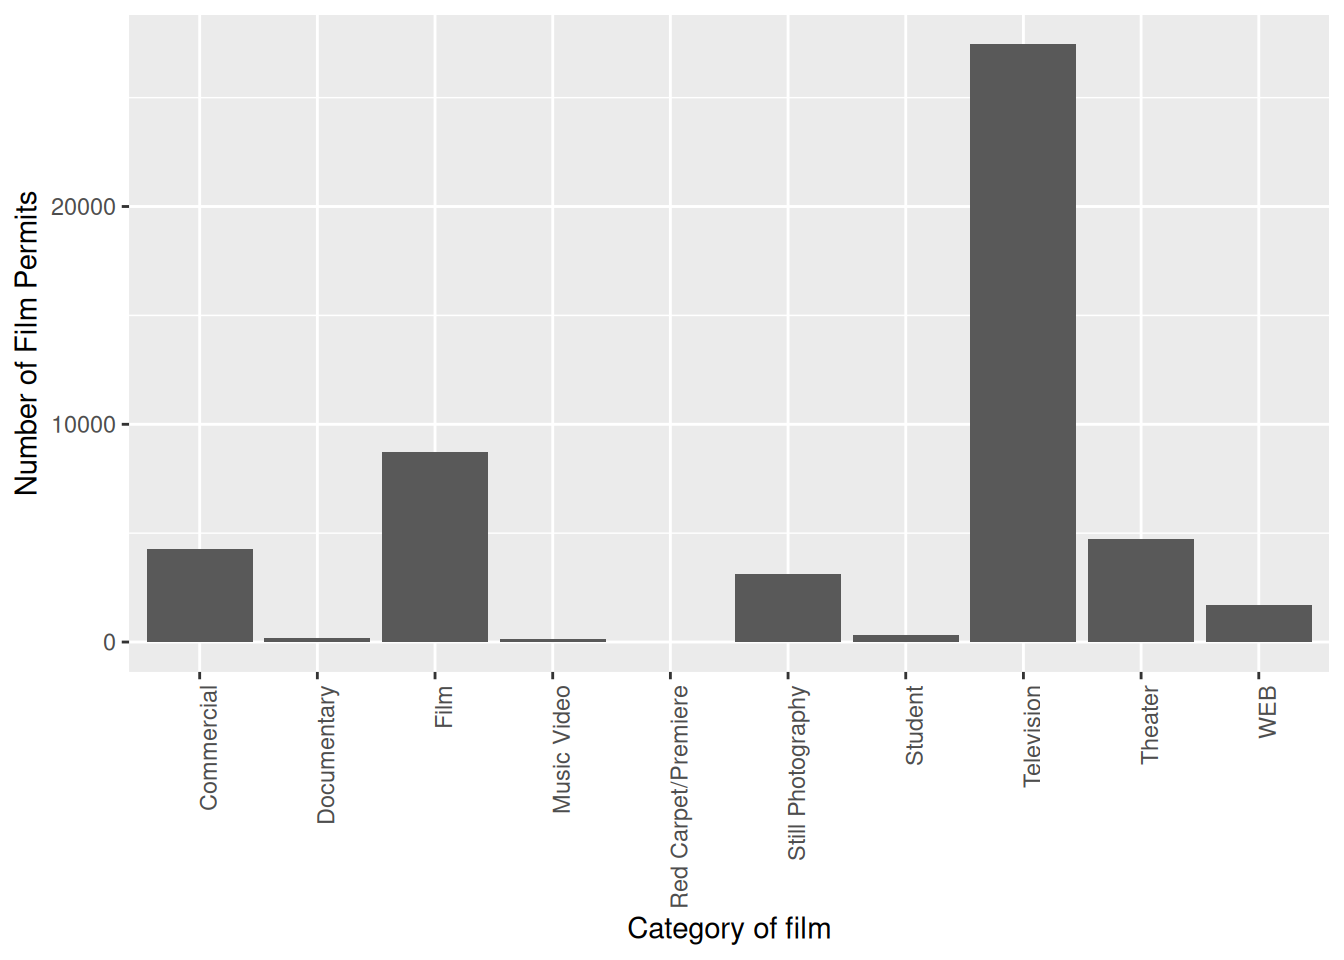
\includegraphics{Statistics_Lab_files/figure-latex/1categoryD-1.pdf}

\hypertarget{ggtitle-adds-title}{%
\subsubsection{ggtitle() adds title}\label{ggtitle-adds-title}}

Let's give our graph a title

\begin{Shaded}
\begin{Highlighting}[]
\FunctionTok{ggplot}\NormalTok{(counts, }\FunctionTok{aes}\NormalTok{(}\AttributeTok{x =}\NormalTok{ Category, }\AttributeTok{y =}\NormalTok{ count\_of\_permits )) }\SpecialCharTok{+}
  \FunctionTok{geom\_bar}\NormalTok{(}\AttributeTok{stat=}\StringTok{"identity"}\NormalTok{) }\SpecialCharTok{+} 
  \FunctionTok{theme}\NormalTok{(}\AttributeTok{axis.text.x =} \FunctionTok{element\_text}\NormalTok{(}\AttributeTok{angle =} \DecValTok{90}\NormalTok{, }\AttributeTok{hjust =} \DecValTok{1}\NormalTok{)) }\SpecialCharTok{+}
  \FunctionTok{ylab}\NormalTok{(}\StringTok{"Number of Film Permits"}\NormalTok{) }\SpecialCharTok{+} 
  \FunctionTok{xlab}\NormalTok{(}\StringTok{"Category of film"}\NormalTok{) }\SpecialCharTok{+}
  \FunctionTok{ggtitle}\NormalTok{(}\StringTok{"Number of Film permits in NYC by Category"}\NormalTok{)}
\end{Highlighting}
\end{Shaded}

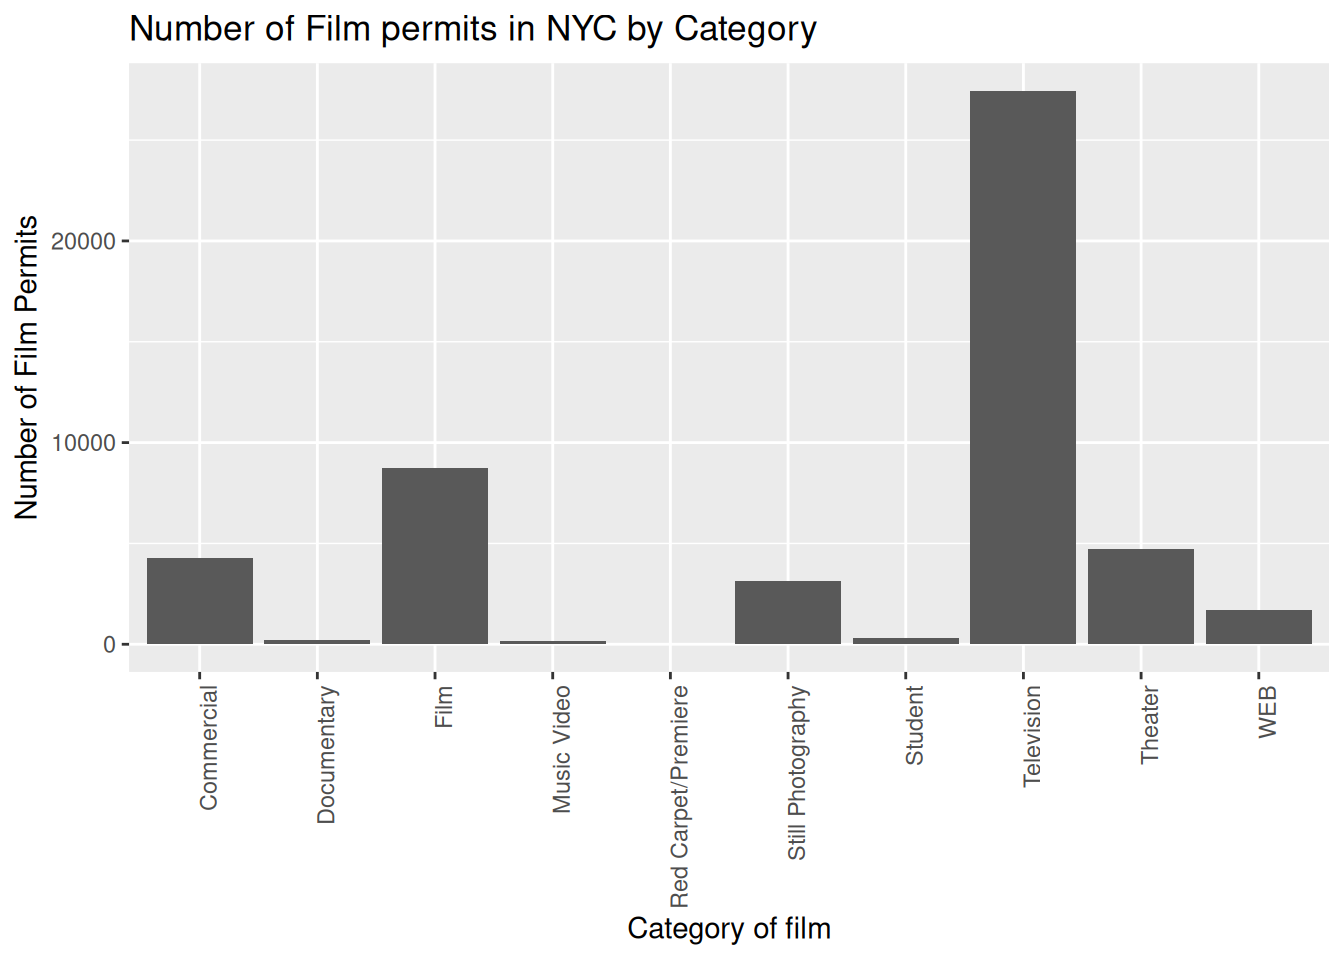
\includegraphics{Statistics_Lab_files/figure-latex/1categoryE-1.pdf}

\hypertarget{color-adds-color}{%
\subsubsection{color adds color}\label{color-adds-color}}

Let's make the bars different colors. To do this, we add new code to the inside of the \texttt{aes()} part:

\begin{Shaded}
\begin{Highlighting}[]
\FunctionTok{ggplot}\NormalTok{(counts, }\FunctionTok{aes}\NormalTok{(}\AttributeTok{x =}\NormalTok{ Category, }\AttributeTok{y =}\NormalTok{ count\_of\_permits, }\AttributeTok{color=}\NormalTok{Category )) }\SpecialCharTok{+}
  \FunctionTok{geom\_bar}\NormalTok{(}\AttributeTok{stat=}\StringTok{"identity"}\NormalTok{) }\SpecialCharTok{+} 
  \FunctionTok{theme}\NormalTok{(}\AttributeTok{axis.text.x =} \FunctionTok{element\_text}\NormalTok{(}\AttributeTok{angle =} \DecValTok{90}\NormalTok{, }\AttributeTok{hjust =} \DecValTok{1}\NormalTok{)) }\SpecialCharTok{+}
  \FunctionTok{ylab}\NormalTok{(}\StringTok{"Number of Film Permits"}\NormalTok{) }\SpecialCharTok{+} 
  \FunctionTok{xlab}\NormalTok{(}\StringTok{"Category of film"}\NormalTok{) }\SpecialCharTok{+}
  \FunctionTok{ggtitle}\NormalTok{(}\StringTok{"Number of Film permits in NYC by Category"}\NormalTok{)}
\end{Highlighting}
\end{Shaded}

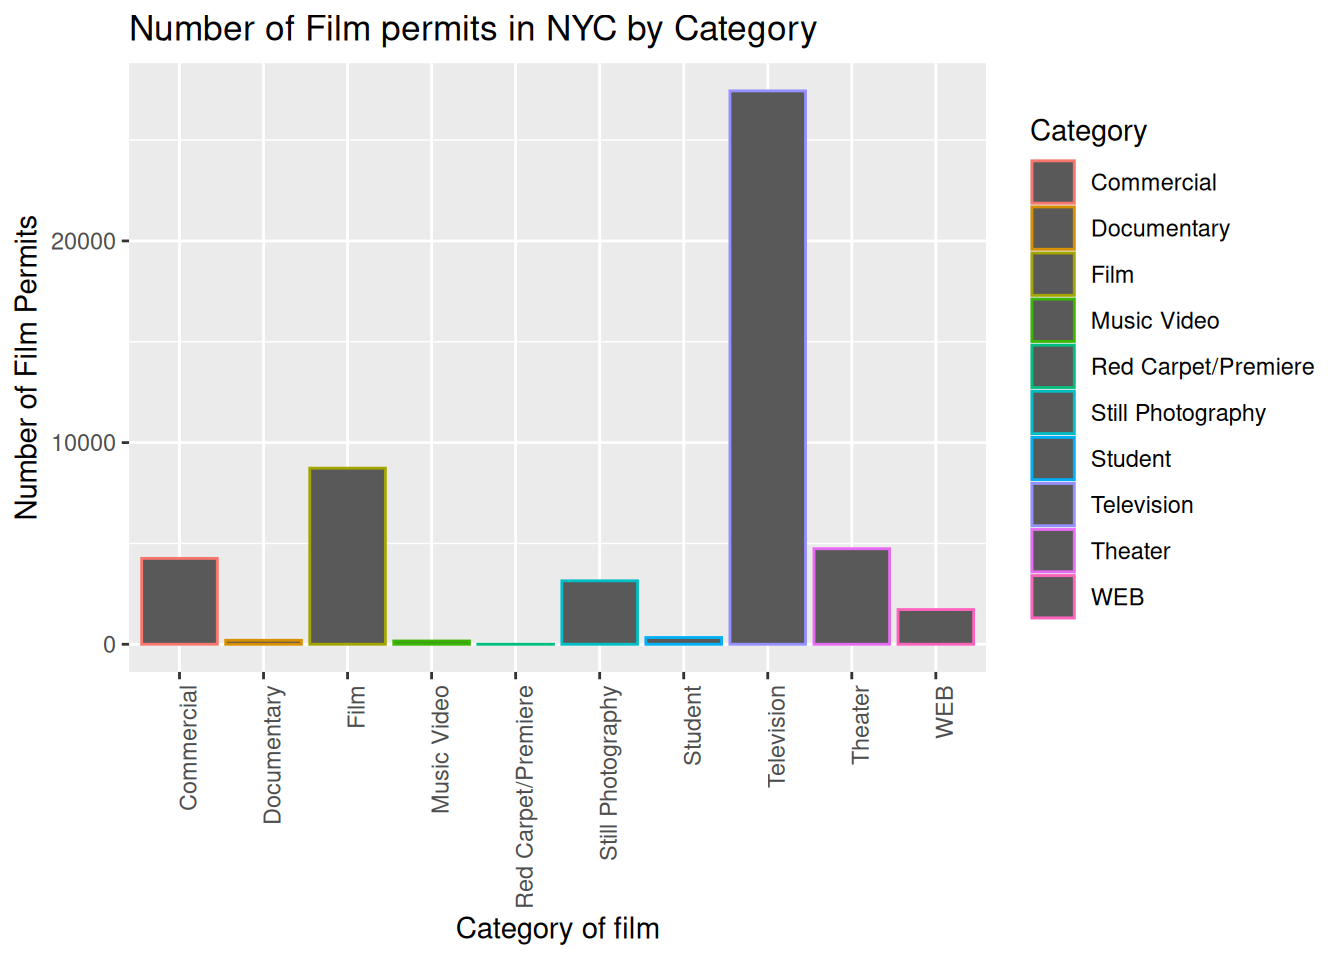
\includegraphics{Statistics_Lab_files/figure-latex/1categoryF-1.pdf}

\hypertarget{fill-fills-in-color}{%
\subsubsection{fill fills in color}\label{fill-fills-in-color}}

Let's make the bars different colors. To do this, we add new code to the inside of the \texttt{aes()} part\ldots Notice I've started using new lines to make the code more readable.

\begin{Shaded}
\begin{Highlighting}[]
\FunctionTok{ggplot}\NormalTok{(counts, }\FunctionTok{aes}\NormalTok{(}\AttributeTok{x =}\NormalTok{ Category, }\AttributeTok{y =}\NormalTok{ count\_of\_permits, }
                   \AttributeTok{color=}\NormalTok{Category, }
                   \AttributeTok{fill=}\NormalTok{ Category )) }\SpecialCharTok{+}
  \FunctionTok{geom\_bar}\NormalTok{(}\AttributeTok{stat=}\StringTok{"identity"}\NormalTok{) }\SpecialCharTok{+} 
  \FunctionTok{theme}\NormalTok{(}\AttributeTok{axis.text.x =} \FunctionTok{element\_text}\NormalTok{(}\AttributeTok{angle =} \DecValTok{90}\NormalTok{, }\AttributeTok{hjust =} \DecValTok{1}\NormalTok{)) }\SpecialCharTok{+}
  \FunctionTok{ylab}\NormalTok{(}\StringTok{"Number of Film Permits"}\NormalTok{) }\SpecialCharTok{+} 
  \FunctionTok{xlab}\NormalTok{(}\StringTok{"Category of film"}\NormalTok{) }\SpecialCharTok{+}
  \FunctionTok{ggtitle}\NormalTok{(}\StringTok{"Number of Film permits in NYC by Category"}\NormalTok{)}
\end{Highlighting}
\end{Shaded}

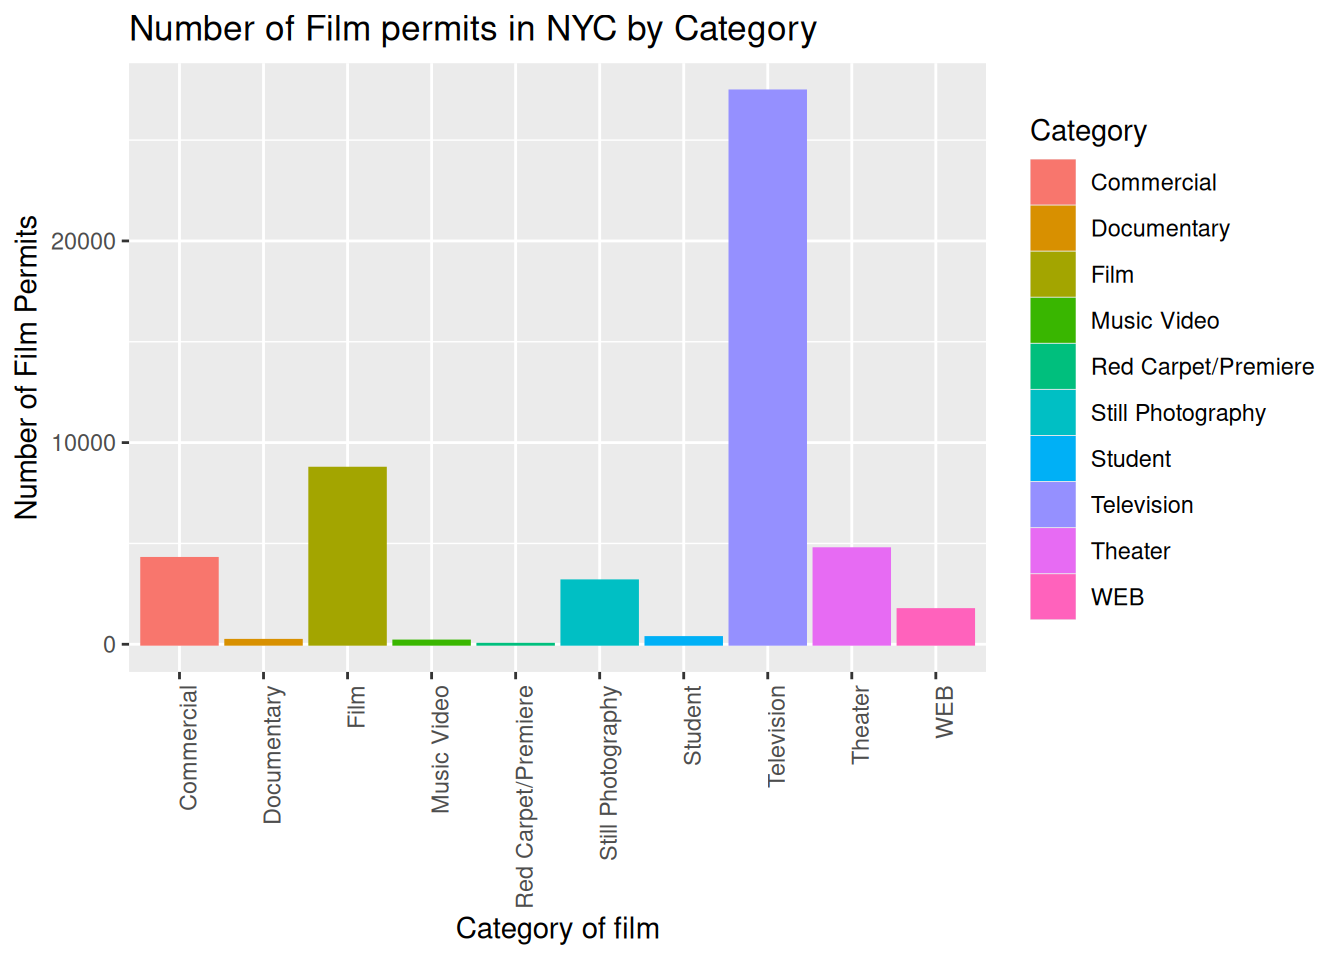
\includegraphics{Statistics_Lab_files/figure-latex/1categoryG-1.pdf}

\hypertarget{get-rid-of-the-legend}{%
\subsubsection{get rid of the legend}\label{get-rid-of-the-legend}}

Sometimes you just don't want the legend on the side, to remove it add

\texttt{theme(legend.position="none")}

\begin{Shaded}
\begin{Highlighting}[]
\FunctionTok{ggplot}\NormalTok{(counts, }\FunctionTok{aes}\NormalTok{(}\AttributeTok{x =}\NormalTok{ Category, }\AttributeTok{y =}\NormalTok{ count\_of\_permits, }
                   \AttributeTok{color=}\NormalTok{Category, }
                   \AttributeTok{fill=}\NormalTok{ Category )) }\SpecialCharTok{+}
  \FunctionTok{geom\_bar}\NormalTok{(}\AttributeTok{stat=}\StringTok{"identity"}\NormalTok{) }\SpecialCharTok{+} 
  \FunctionTok{theme}\NormalTok{(}\AttributeTok{axis.text.x =} \FunctionTok{element\_text}\NormalTok{(}\AttributeTok{angle =} \DecValTok{90}\NormalTok{, }\AttributeTok{hjust =} \DecValTok{1}\NormalTok{)) }\SpecialCharTok{+}
  \FunctionTok{ylab}\NormalTok{(}\StringTok{"Number of Film Permits"}\NormalTok{) }\SpecialCharTok{+} 
  \FunctionTok{xlab}\NormalTok{(}\StringTok{"Category of film"}\NormalTok{) }\SpecialCharTok{+}
  \FunctionTok{ggtitle}\NormalTok{(}\StringTok{"Number of Film permits in NYC by Category"}\NormalTok{) }\SpecialCharTok{+}
  \FunctionTok{theme}\NormalTok{(}\AttributeTok{legend.position=}\StringTok{"none"}\NormalTok{)}
\end{Highlighting}
\end{Shaded}

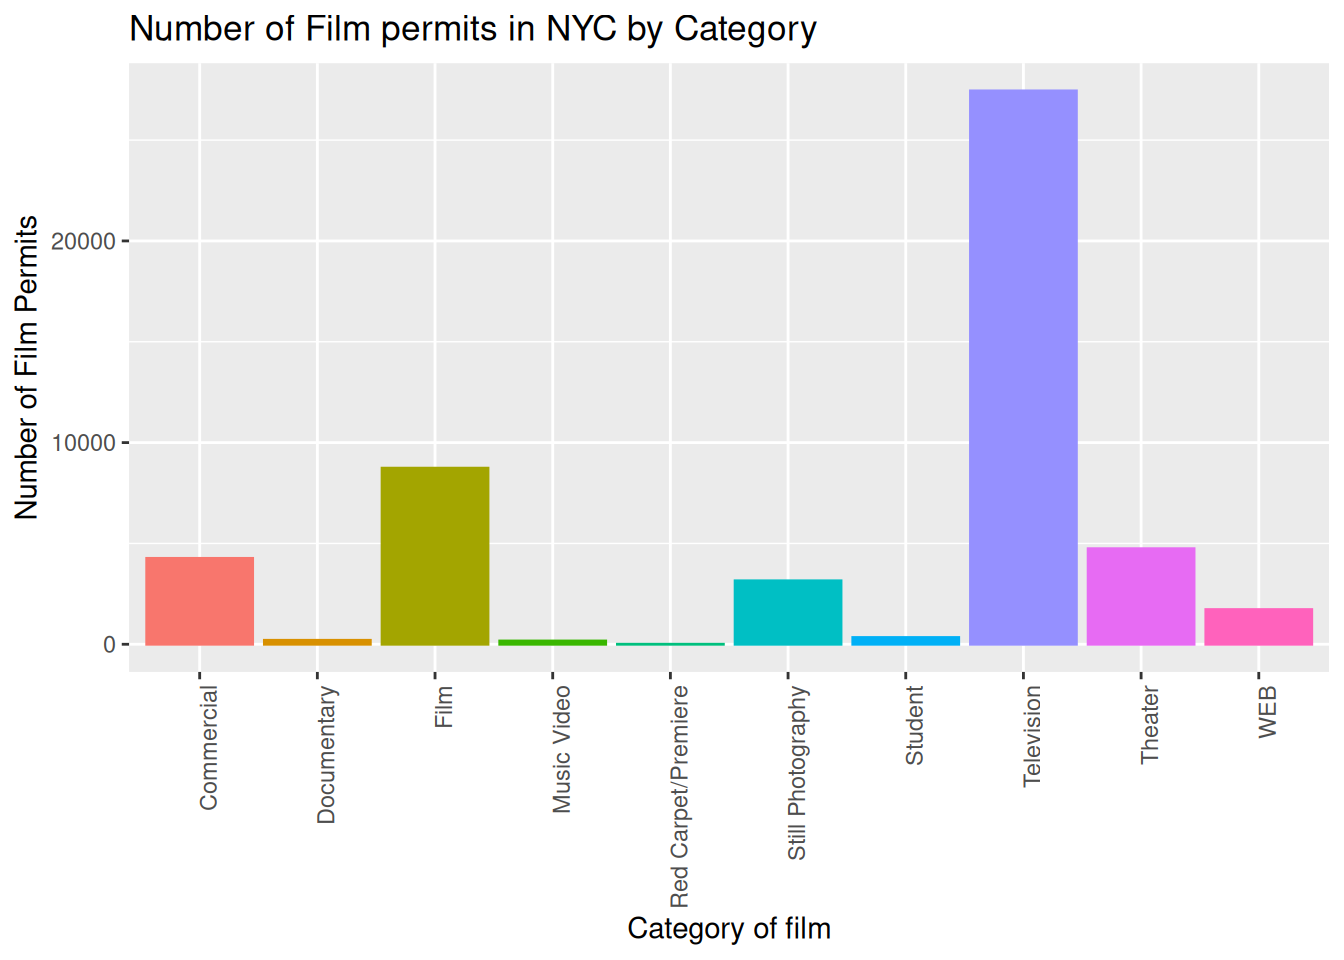
\includegraphics{Statistics_Lab_files/figure-latex/1categoryH-1.pdf}

\hypertarget{theme_classic-makes-white-background}{%
\subsubsection{theme\_classic() makes white background}\label{theme_classic-makes-white-background}}

The rest is often just visual preference. For example, the graph above has this grey grid behind the bars. For a clean classic no nonsense look, use \texttt{theme\_classic()} to take away the grid.

\begin{Shaded}
\begin{Highlighting}[]
\FunctionTok{ggplot}\NormalTok{(counts, }\FunctionTok{aes}\NormalTok{(}\AttributeTok{x =}\NormalTok{ Category, }\AttributeTok{y =}\NormalTok{ count\_of\_permits, }
                   \AttributeTok{color=}\NormalTok{Category, }
                   \AttributeTok{fill=}\NormalTok{ Category )) }\SpecialCharTok{+}
  \FunctionTok{geom\_bar}\NormalTok{(}\AttributeTok{stat=}\StringTok{"identity"}\NormalTok{) }\SpecialCharTok{+} 
  \FunctionTok{theme}\NormalTok{(}\AttributeTok{axis.text.x =} \FunctionTok{element\_text}\NormalTok{(}\AttributeTok{angle =} \DecValTok{90}\NormalTok{, }\AttributeTok{hjust =} \DecValTok{1}\NormalTok{)) }\SpecialCharTok{+}
  \FunctionTok{ylab}\NormalTok{(}\StringTok{"Number of Film Permits"}\NormalTok{) }\SpecialCharTok{+} 
  \FunctionTok{xlab}\NormalTok{(}\StringTok{"Category of film"}\NormalTok{) }\SpecialCharTok{+}
  \FunctionTok{ggtitle}\NormalTok{(}\StringTok{"Number of Film permits in NYC by Category"}\NormalTok{) }\SpecialCharTok{+}
  \FunctionTok{theme}\NormalTok{(}\AttributeTok{legend.position=}\StringTok{"none"}\NormalTok{) }\SpecialCharTok{+}
  \FunctionTok{theme\_classic}\NormalTok{()}
\end{Highlighting}
\end{Shaded}

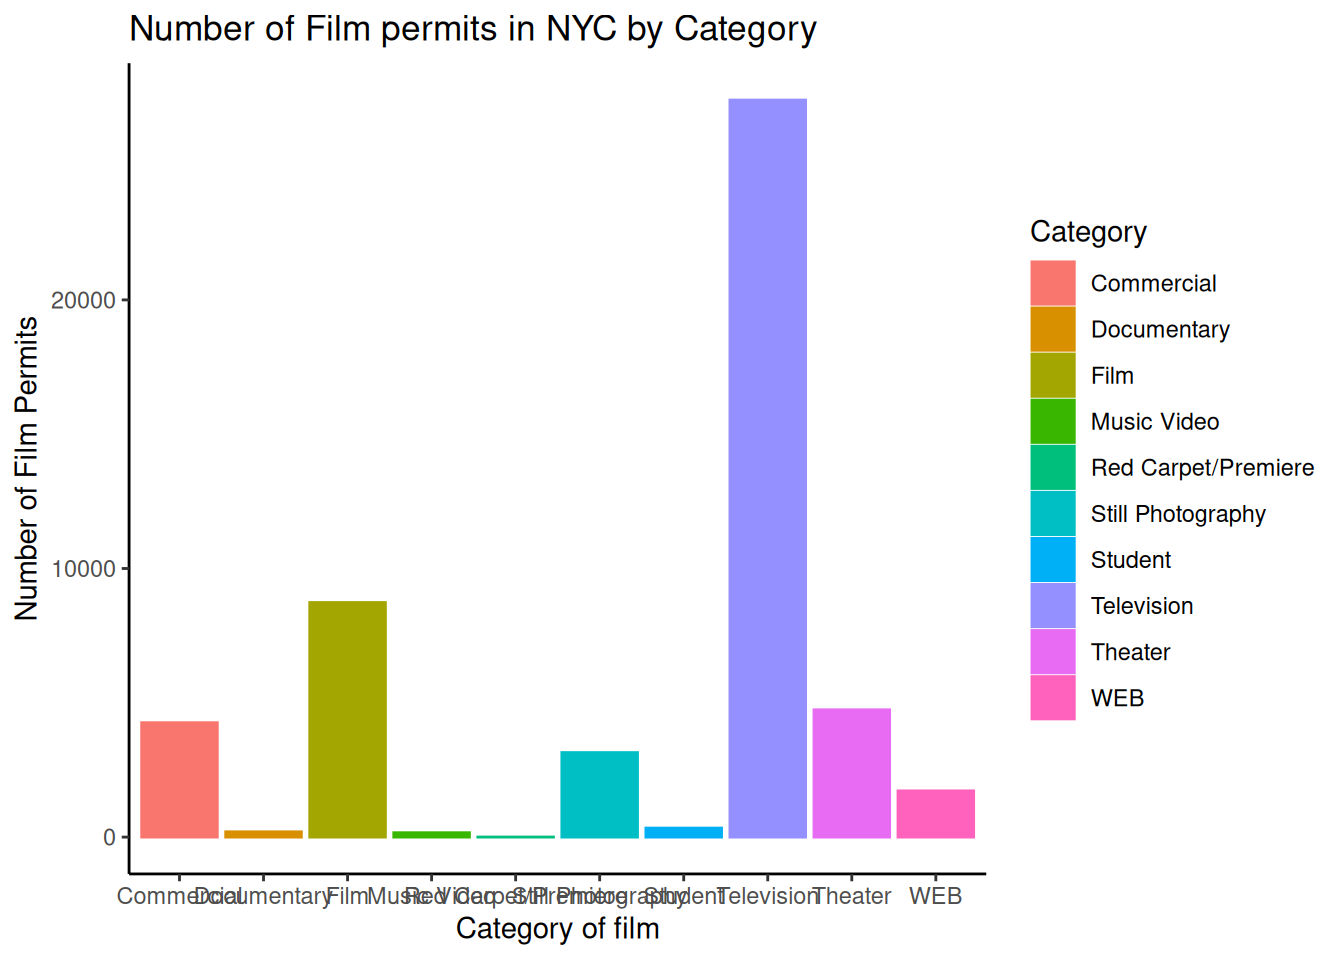
\includegraphics{Statistics_Lab_files/figure-latex/1categoryI-1.pdf}

\hypertarget{sometimes-layer-order-matters}{%
\subsubsection{Sometimes layer order matters}\label{sometimes-layer-order-matters}}

Interesting, \texttt{theme\_classic()} is misbehaving a little bit. It looks like we have some of our layer out of order, let's re-order. I just moved \texttt{theme\_classic()} to just underneath the \texttt{geom\_bar()} line. Now everything get's drawn properly.

\begin{Shaded}
\begin{Highlighting}[]
\FunctionTok{ggplot}\NormalTok{(counts, }\FunctionTok{aes}\NormalTok{(}\AttributeTok{x =}\NormalTok{ Category, }\AttributeTok{y =}\NormalTok{ count\_of\_permits, }
                   \AttributeTok{color=}\NormalTok{Category, }
                   \AttributeTok{fill=}\NormalTok{ Category )) }\SpecialCharTok{+}
  \FunctionTok{geom\_bar}\NormalTok{(}\AttributeTok{stat=}\StringTok{"identity"}\NormalTok{) }\SpecialCharTok{+} 
  \FunctionTok{theme\_classic}\NormalTok{() }\SpecialCharTok{+}
  \FunctionTok{theme}\NormalTok{(}\AttributeTok{axis.text.x =} \FunctionTok{element\_text}\NormalTok{(}\AttributeTok{angle =} \DecValTok{90}\NormalTok{, }\AttributeTok{hjust =} \DecValTok{1}\NormalTok{)) }\SpecialCharTok{+}
  \FunctionTok{ylab}\NormalTok{(}\StringTok{"Number of Film Permits"}\NormalTok{) }\SpecialCharTok{+} 
  \FunctionTok{xlab}\NormalTok{(}\StringTok{"Category of film"}\NormalTok{) }\SpecialCharTok{+}
  \FunctionTok{ggtitle}\NormalTok{(}\StringTok{"Number of Film permits in NYC by Category"}\NormalTok{) }\SpecialCharTok{+}
  \FunctionTok{theme}\NormalTok{(}\AttributeTok{legend.position=}\StringTok{"none"}\NormalTok{) }
\end{Highlighting}
\end{Shaded}

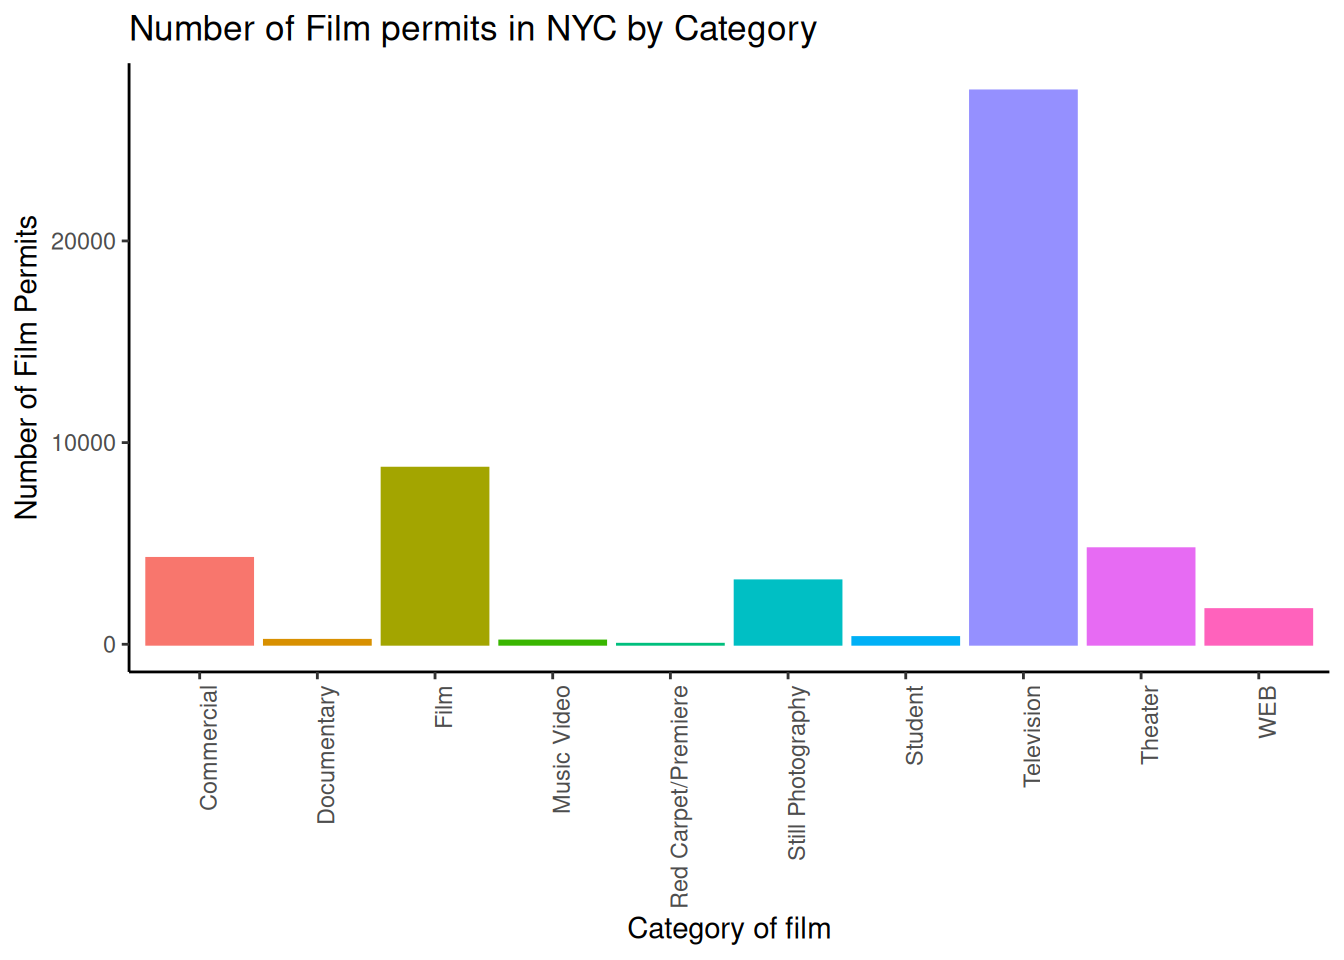
\includegraphics{Statistics_Lab_files/figure-latex/1categoryJ-1.pdf}

\hypertarget{font-size}{%
\subsubsection{Font-size}\label{font-size}}

Changing font-size is often something you want to do. ggplot2 can do this in different ways. I suggest using the \texttt{base\_size} option inside \texttt{theme\_classic()}. You set one number for the largest font size in the graph, and everything else gets scaled to fit with that that first number. It's really convenient. Look for the inside of \texttt{theme\_classic()}

\begin{Shaded}
\begin{Highlighting}[]
\FunctionTok{ggplot}\NormalTok{(counts, }\FunctionTok{aes}\NormalTok{(}\AttributeTok{x =}\NormalTok{ Category, }\AttributeTok{y =}\NormalTok{ count\_of\_permits, }
                   \AttributeTok{color=}\NormalTok{Category, }
                   \AttributeTok{fill=}\NormalTok{ Category )) }\SpecialCharTok{+}
  \FunctionTok{geom\_bar}\NormalTok{(}\AttributeTok{stat=}\StringTok{"identity"}\NormalTok{) }\SpecialCharTok{+} 
  \FunctionTok{theme\_classic}\NormalTok{(}\AttributeTok{base\_size =} \DecValTok{15}\NormalTok{) }\SpecialCharTok{+}
  \FunctionTok{theme}\NormalTok{(}\AttributeTok{axis.text.x =} \FunctionTok{element\_text}\NormalTok{(}\AttributeTok{angle =} \DecValTok{90}\NormalTok{, }\AttributeTok{hjust =} \DecValTok{1}\NormalTok{)) }\SpecialCharTok{+}
  \FunctionTok{ylab}\NormalTok{(}\StringTok{"Number of Film Permits"}\NormalTok{) }\SpecialCharTok{+} 
  \FunctionTok{xlab}\NormalTok{(}\StringTok{"Category of film"}\NormalTok{) }\SpecialCharTok{+}
  \FunctionTok{ggtitle}\NormalTok{(}\StringTok{"Number of Film permits in NYC by Category"}\NormalTok{) }\SpecialCharTok{+}
  \FunctionTok{theme}\NormalTok{(}\AttributeTok{legend.position=}\StringTok{"none"}\NormalTok{) }
\end{Highlighting}
\end{Shaded}

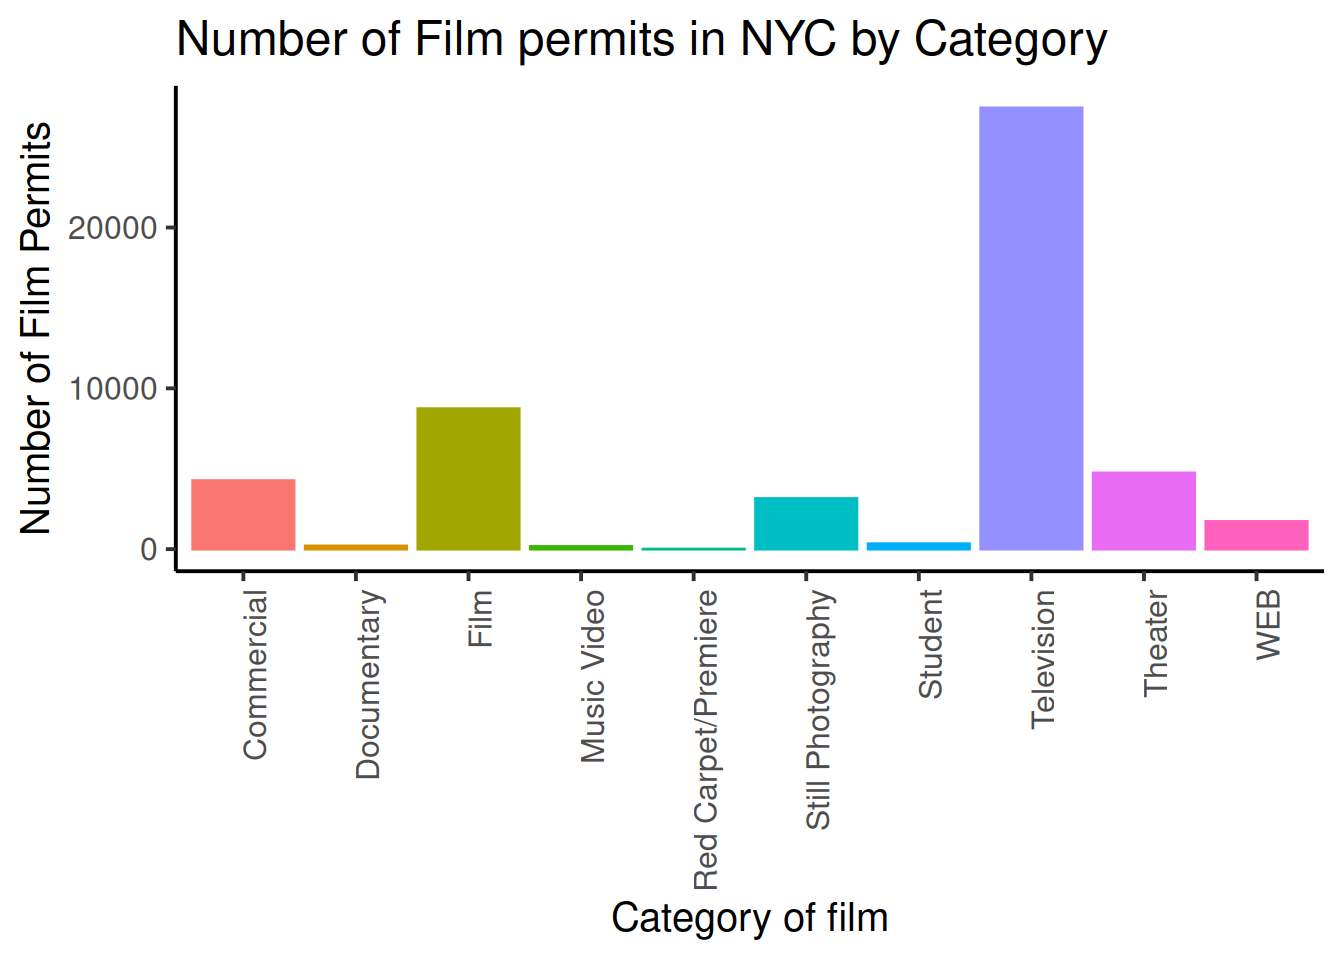
\includegraphics{Statistics_Lab_files/figure-latex/1categoryK-1.pdf}
or make things small\ldots{} just to see what happens

\begin{Shaded}
\begin{Highlighting}[]
\FunctionTok{ggplot}\NormalTok{(counts, }\FunctionTok{aes}\NormalTok{(}\AttributeTok{x =}\NormalTok{ Category, }\AttributeTok{y =}\NormalTok{ count\_of\_permits, }
                   \AttributeTok{color=}\NormalTok{Category, }
                   \AttributeTok{fill=}\NormalTok{ Category )) }\SpecialCharTok{+}
  \FunctionTok{geom\_bar}\NormalTok{(}\AttributeTok{stat=}\StringTok{"identity"}\NormalTok{) }\SpecialCharTok{+} 
  \FunctionTok{theme\_classic}\NormalTok{(}\AttributeTok{base\_size =} \DecValTok{10}\NormalTok{) }\SpecialCharTok{+}
  \FunctionTok{theme}\NormalTok{(}\AttributeTok{axis.text.x =} \FunctionTok{element\_text}\NormalTok{(}\AttributeTok{angle =} \DecValTok{90}\NormalTok{, }\AttributeTok{hjust =} \DecValTok{1}\NormalTok{)) }\SpecialCharTok{+}
  \FunctionTok{ylab}\NormalTok{(}\StringTok{"Number of Film Permits"}\NormalTok{) }\SpecialCharTok{+} 
  \FunctionTok{xlab}\NormalTok{(}\StringTok{"Category of film"}\NormalTok{) }\SpecialCharTok{+}
  \FunctionTok{ggtitle}\NormalTok{(}\StringTok{"Number of Film permits in NYC by Category"}\NormalTok{) }\SpecialCharTok{+}
  \FunctionTok{theme}\NormalTok{(}\AttributeTok{legend.position=}\StringTok{"none"}\NormalTok{) }
\end{Highlighting}
\end{Shaded}

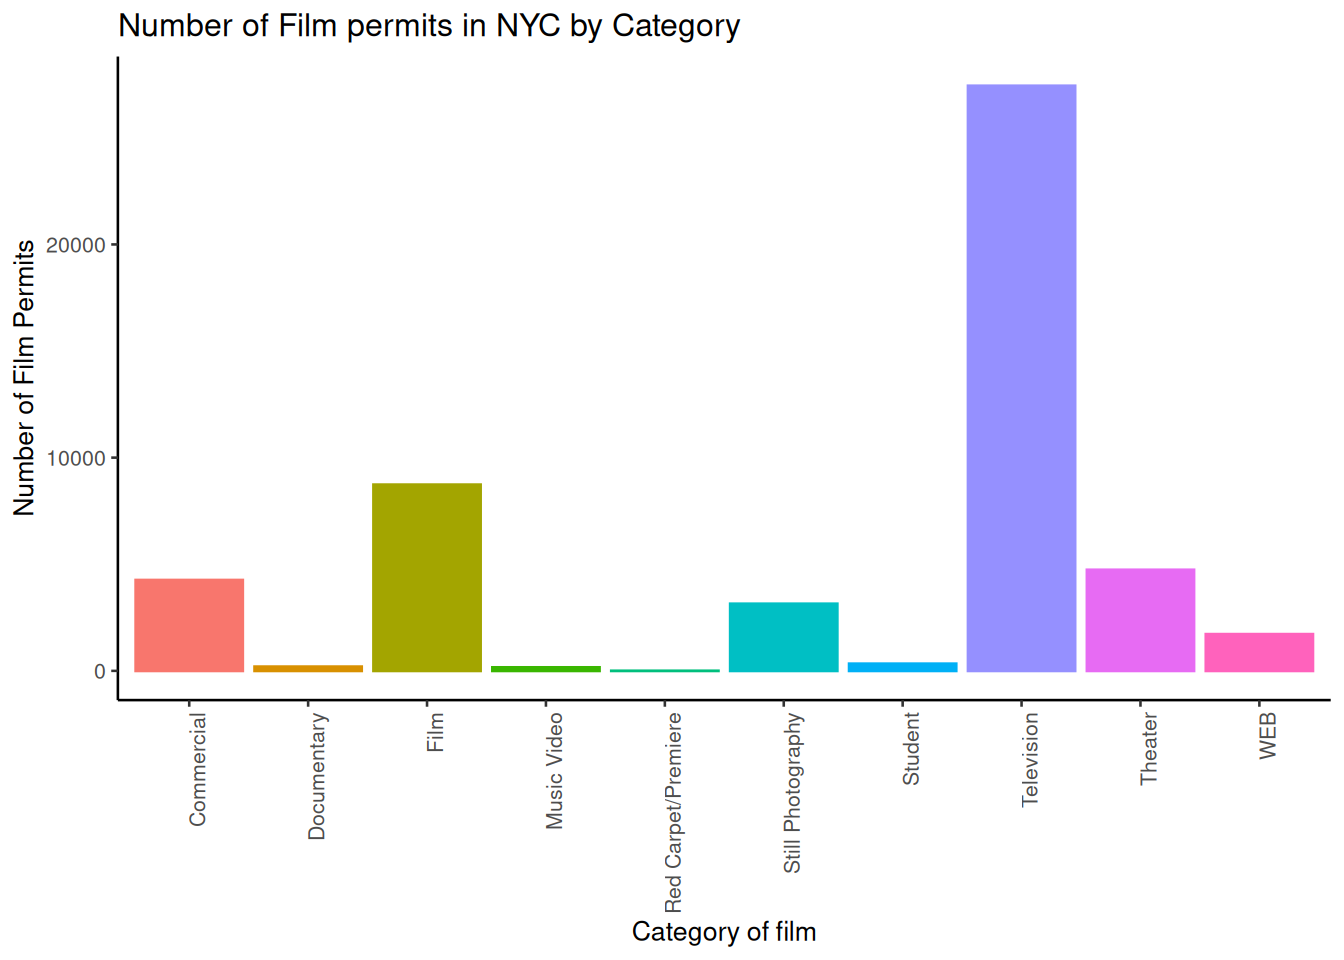
\includegraphics{Statistics_Lab_files/figure-latex/1categoryL-1.pdf}

\hypertarget{ggplot2-summary}{%
\subsubsection{ggplot2 summary}\label{ggplot2-summary}}

That's enough of the ggplot2 basics for now. You will discover that many things are possible with ggplot2. It is amazing. We are going to get back to answering some questions about the data with graphs. But, now that we have built the code to make the graphs, all we need to do is copy-paste, and make a few small changes, and boom, we have our graph.

\hypertarget{more-questions-about-nyc-films}{%
\subsection{More questions about NYC films}\label{more-questions-about-nyc-films}}

\hypertarget{what-are-the-sub-categories-of-films}{%
\subsubsection{What are the sub-categories of films?}\label{what-are-the-sub-categories-of-films}}

Notice the \texttt{nyc\_films} data frame also has a column for \texttt{SubCategoryName}. Let's see what's going on there with a quick plot.

\begin{Shaded}
\begin{Highlighting}[]
\CommentTok{\# get the counts (this is a comment it\textquotesingle{}s just here for you to read)}

\NormalTok{counts }\OtherTok{\textless{}{-}}\NormalTok{ nyc\_films }\SpecialCharTok{\%\textgreater{}\%}
          \FunctionTok{group\_by}\NormalTok{(SubCategoryName) }\SpecialCharTok{\%\textgreater{}\%}
          \FunctionTok{summarize}\NormalTok{(}\AttributeTok{count\_of\_permits =} \FunctionTok{length}\NormalTok{(SubCategoryName))}

\CommentTok{\# make the plot}

\FunctionTok{ggplot}\NormalTok{(counts, }\FunctionTok{aes}\NormalTok{(}\AttributeTok{x =}\NormalTok{ SubCategoryName, }\AttributeTok{y =}\NormalTok{ count\_of\_permits, }
                   \AttributeTok{color=}\NormalTok{SubCategoryName, }
                   \AttributeTok{fill=}\NormalTok{ SubCategoryName )) }\SpecialCharTok{+}
  \FunctionTok{geom\_bar}\NormalTok{(}\AttributeTok{stat=}\StringTok{"identity"}\NormalTok{) }\SpecialCharTok{+} 
  \FunctionTok{theme\_classic}\NormalTok{(}\AttributeTok{base\_size =} \DecValTok{10}\NormalTok{) }\SpecialCharTok{+}
  \FunctionTok{theme}\NormalTok{(}\AttributeTok{axis.text.x =} \FunctionTok{element\_text}\NormalTok{(}\AttributeTok{angle =} \DecValTok{90}\NormalTok{, }\AttributeTok{hjust =} \DecValTok{1}\NormalTok{)) }\SpecialCharTok{+}
  \FunctionTok{ylab}\NormalTok{(}\StringTok{"Number of Film Permits"}\NormalTok{) }\SpecialCharTok{+} 
  \FunctionTok{xlab}\NormalTok{(}\StringTok{"Sub{-}category of film"}\NormalTok{) }\SpecialCharTok{+}
  \FunctionTok{ggtitle}\NormalTok{(}\StringTok{"Number of Film permits in NYC by Sub{-}category"}\NormalTok{) }\SpecialCharTok{+}
  \FunctionTok{theme}\NormalTok{(}\AttributeTok{legend.position=}\StringTok{"none"}\NormalTok{) }
\end{Highlighting}
\end{Shaded}

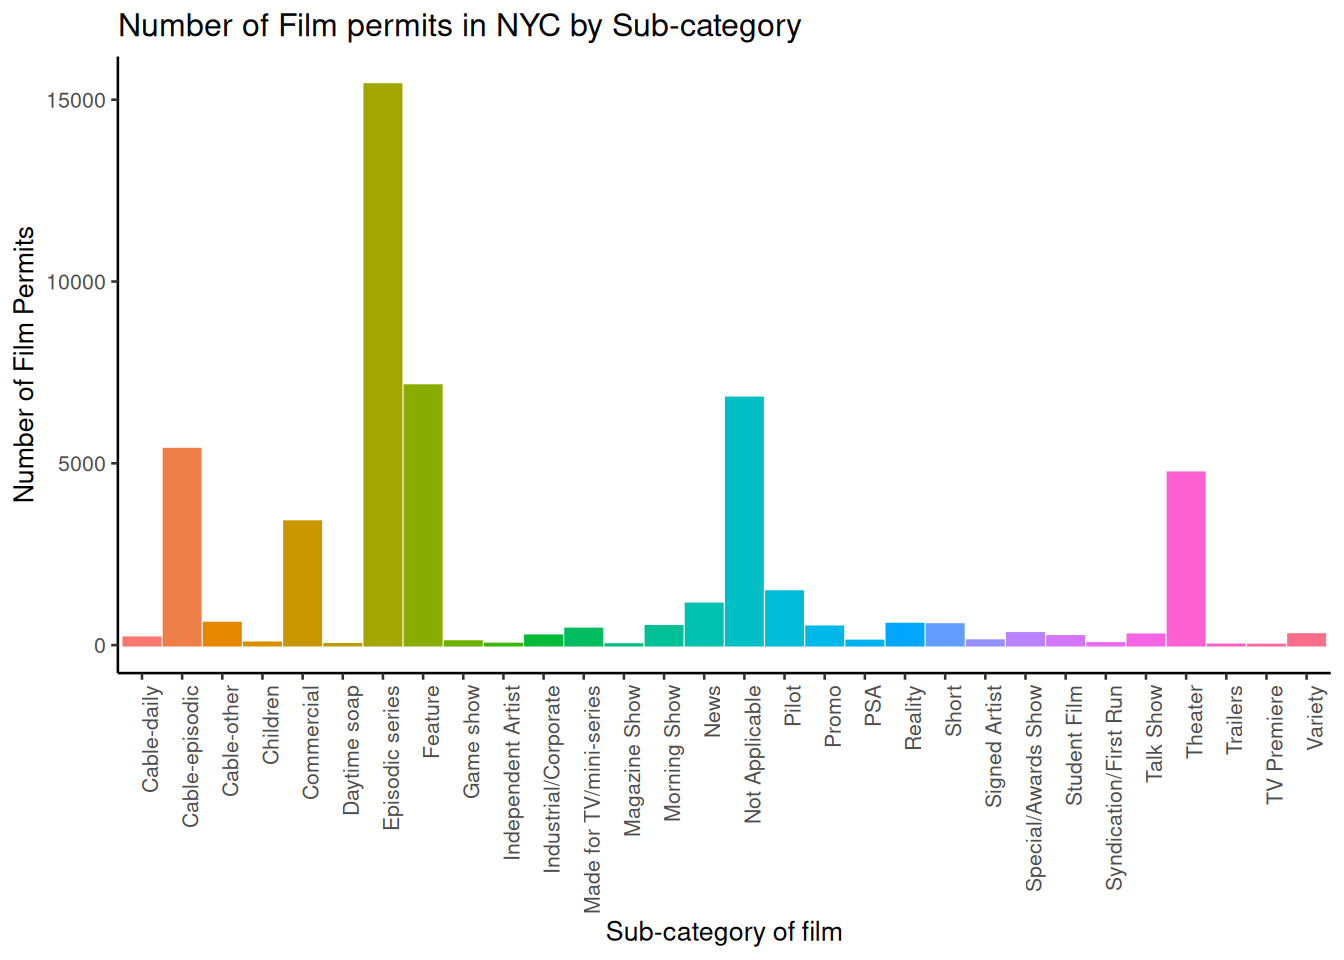
\includegraphics{Statistics_Lab_files/figure-latex/1subcategory-1.pdf}

I guess ``episodic series'' are the most common. Using a graph like this gave us our answer super fast.

\hypertarget{categories-by-different-boroughs}{%
\subsubsection{Categories by different Boroughs}\label{categories-by-different-boroughs}}

Let's see one more really useful thing about ggplot2. It's called \texttt{facet\_wrap()}. It's an ugly word, but you will see that it is very cool, and you can do next-level-super-hero graph styles with \texttt{facet\_wrap} that other people can't do very easily.

Here's our question. We know that some films are made in different Boroughs, and that same films are made in different categories, but do different Boroughs have different patterns for the kinds of categories of films they request permits for? Are their more TV shows in Brooklyn? How do we find out? Watch, just like this:

\begin{Shaded}
\begin{Highlighting}[]
\CommentTok{\# get the counts (this is a comment it\textquotesingle{}s just here for you to read)}

\NormalTok{counts }\OtherTok{\textless{}{-}}\NormalTok{ nyc\_films }\SpecialCharTok{\%\textgreater{}\%}
          \FunctionTok{group\_by}\NormalTok{(Borough,Category) }\SpecialCharTok{\%\textgreater{}\%}
          \FunctionTok{summarize}\NormalTok{(}\AttributeTok{count\_of\_permits =} \FunctionTok{length}\NormalTok{(Category))}

\CommentTok{\# make the plot}

\FunctionTok{ggplot}\NormalTok{(counts, }\FunctionTok{aes}\NormalTok{(}\AttributeTok{x =}\NormalTok{ Category, }\AttributeTok{y =}\NormalTok{ count\_of\_permits, }
                   \AttributeTok{color=}\NormalTok{Category, }
                   \AttributeTok{fill=}\NormalTok{ Category )) }\SpecialCharTok{+}
  \FunctionTok{geom\_bar}\NormalTok{(}\AttributeTok{stat=}\StringTok{"identity"}\NormalTok{) }\SpecialCharTok{+} 
  \FunctionTok{theme\_classic}\NormalTok{(}\AttributeTok{base\_size =} \DecValTok{10}\NormalTok{) }\SpecialCharTok{+}
  \FunctionTok{theme}\NormalTok{(}\AttributeTok{axis.text.x =} \FunctionTok{element\_text}\NormalTok{(}\AttributeTok{angle =} \DecValTok{90}\NormalTok{, }\AttributeTok{hjust =} \DecValTok{1}\NormalTok{)) }\SpecialCharTok{+}
  \FunctionTok{ylab}\NormalTok{(}\StringTok{"Number of Film Permits"}\NormalTok{) }\SpecialCharTok{+} 
  \FunctionTok{xlab}\NormalTok{(}\StringTok{"Category of film"}\NormalTok{) }\SpecialCharTok{+}
  \FunctionTok{ggtitle}\NormalTok{(}\StringTok{"Number of Film permits in NYC by Category and Borough"}\NormalTok{) }\SpecialCharTok{+}
  \FunctionTok{theme}\NormalTok{(}\AttributeTok{legend.position=}\StringTok{"none"}\NormalTok{) }\SpecialCharTok{+}
  \FunctionTok{facet\_wrap}\NormalTok{(}\SpecialCharTok{\textasciitilde{}}\NormalTok{Borough, }\AttributeTok{ncol=}\DecValTok{3}\NormalTok{)}
\end{Highlighting}
\end{Shaded}

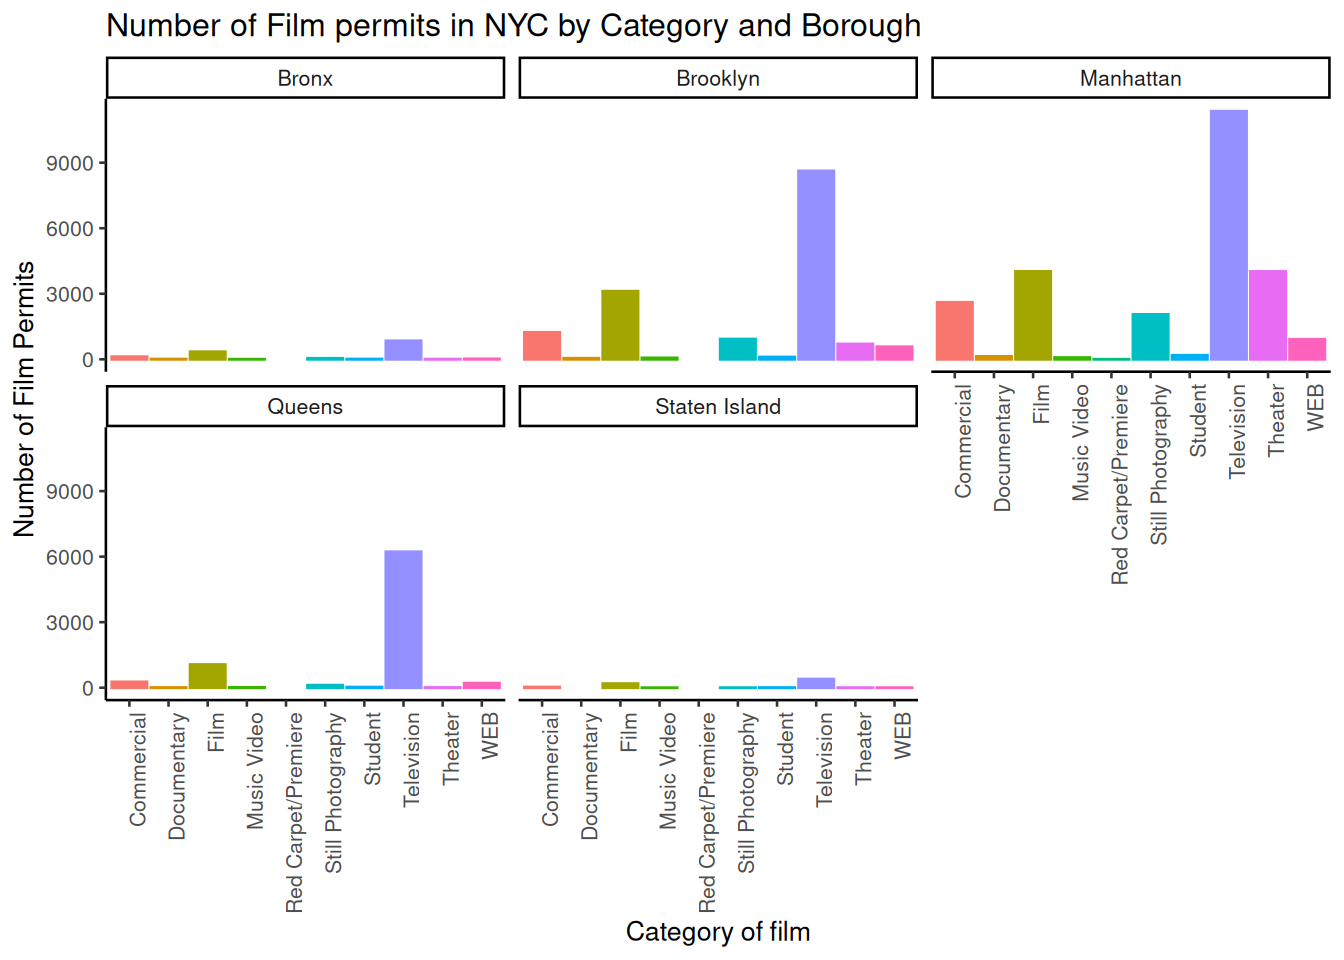
\includegraphics{Statistics_Lab_files/figure-latex/1facetwrap-1.pdf}

We did two important things. First we added \texttt{Borough} and \texttt{Category} into the \texttt{group\_by()} function. This automatically gives separate counts for each category of film, for each Borough. Then we added \texttt{facet\_wrap(\textasciitilde{}Borough,\ ncol=3)} to the end of the plot, and it automatically drew us 5 different bar graphs, one for each Borough! That was fast. Imagine doing that by hand.

The nice thing about this is we can switch things around if we want. For example, we could do it this way by switching the \texttt{Category} with \texttt{Borough}, and facet-wrapping by Category instead of Borough like we did above. Do what works for you.

\begin{Shaded}
\begin{Highlighting}[]
\FunctionTok{ggplot}\NormalTok{(counts, }\FunctionTok{aes}\NormalTok{(}\AttributeTok{x =}\NormalTok{ Borough, }\AttributeTok{y =}\NormalTok{ count\_of\_permits, }
                   \AttributeTok{color=}\NormalTok{Borough, }
                   \AttributeTok{fill=}\NormalTok{ Borough )) }\SpecialCharTok{+}
  \FunctionTok{geom\_bar}\NormalTok{(}\AttributeTok{stat=}\StringTok{"identity"}\NormalTok{) }\SpecialCharTok{+} 
  \FunctionTok{theme\_classic}\NormalTok{(}\AttributeTok{base\_size =} \DecValTok{10}\NormalTok{) }\SpecialCharTok{+}
  \FunctionTok{theme}\NormalTok{(}\AttributeTok{axis.text.x =} \FunctionTok{element\_text}\NormalTok{(}\AttributeTok{angle =} \DecValTok{90}\NormalTok{, }\AttributeTok{hjust =} \DecValTok{1}\NormalTok{)) }\SpecialCharTok{+}
  \FunctionTok{ylab}\NormalTok{(}\StringTok{"Number of Film Permits"}\NormalTok{) }\SpecialCharTok{+} 
  \FunctionTok{xlab}\NormalTok{(}\StringTok{"Borough"}\NormalTok{) }\SpecialCharTok{+}
  \FunctionTok{ggtitle}\NormalTok{(}\StringTok{"Number of Film permits in NYC by Category and Borough"}\NormalTok{) }\SpecialCharTok{+}
  \FunctionTok{theme}\NormalTok{(}\AttributeTok{legend.position=}\StringTok{"none"}\NormalTok{) }\SpecialCharTok{+}
  \FunctionTok{facet\_wrap}\NormalTok{(}\SpecialCharTok{\textasciitilde{}}\NormalTok{Category, }\AttributeTok{ncol=}\DecValTok{5}\NormalTok{)}
\end{Highlighting}
\end{Shaded}

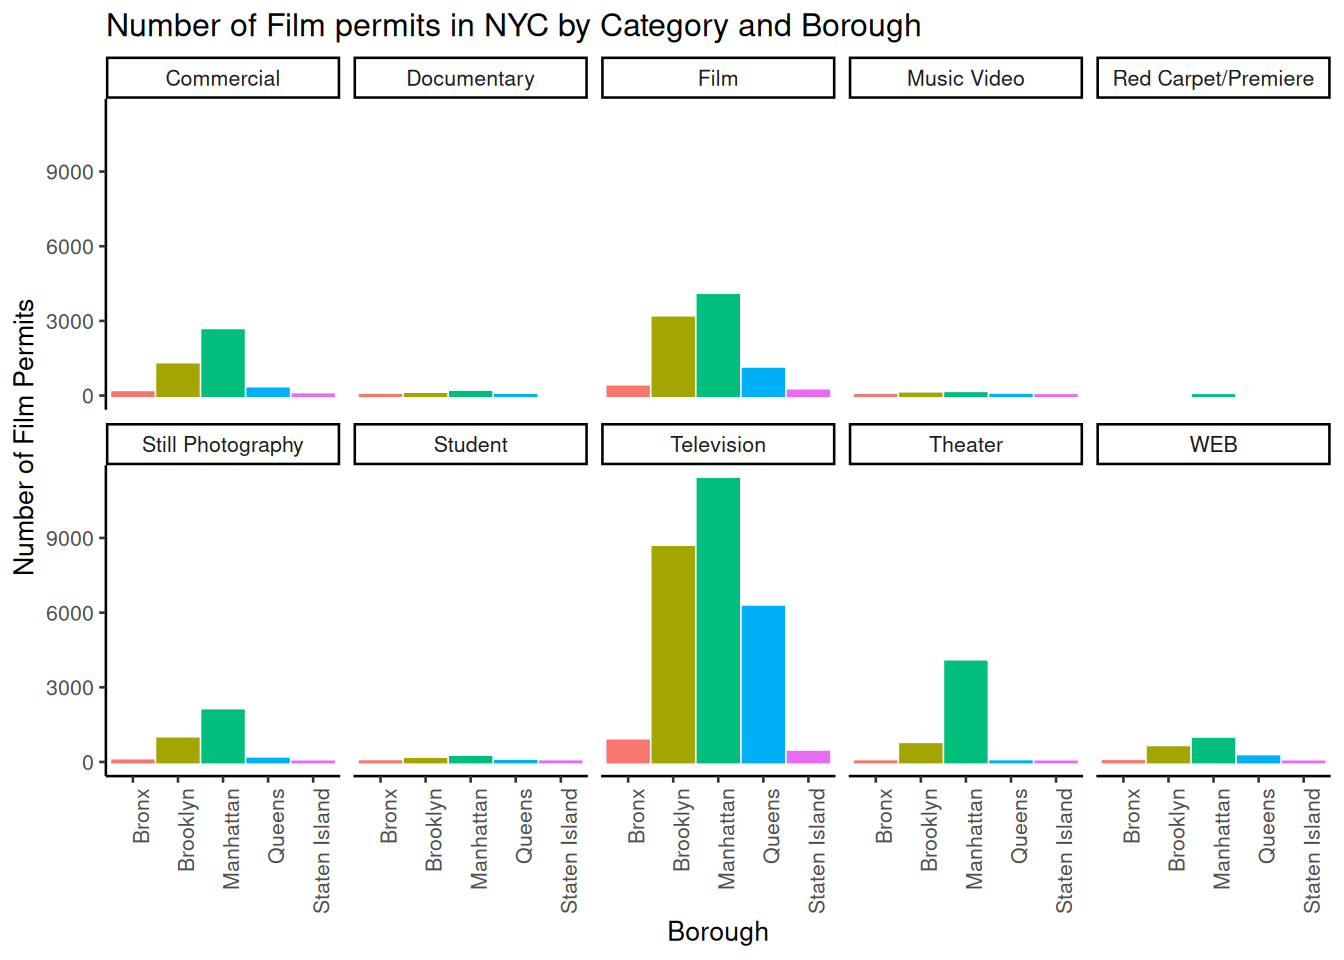
\includegraphics{Statistics_Lab_files/figure-latex/1facetwrap2-1.pdf}

\hypertarget{gapminder-data}{%
\subsection{Gapminder Data}\label{gapminder-data}}

\url{https://www.gapminder.org} is an organization that collects some really interesting worldwide data. They also make cool visualization tools for looking at the data. There are many neat examples, and they have visualization tools built right into their website that you can play around with \url{https://www.gapminder.org/tools/}. That's fun check it out.

There is also an R package called \texttt{gapminder}. When you install this package, it loads in some of the data from gapminder, so we can play with it in R.

If you don't have the gapminder package installed, you can install it by running this code

\begin{Shaded}
\begin{Highlighting}[]
\FunctionTok{install.packages}\NormalTok{(}\StringTok{"gapminder"}\NormalTok{)}
\end{Highlighting}
\end{Shaded}

Once the package is installed, you need to load the new library, like this. Then, you can put the \texttt{gapminder} data into a data frame, like we do here: \texttt{gapminder\_df}.

\begin{Shaded}
\begin{Highlighting}[]
\FunctionTok{library}\NormalTok{(gapminder)}
\NormalTok{gapminder\_df}\OtherTok{\textless{}{-}}\NormalTok{gapminder}
\end{Highlighting}
\end{Shaded}

\hypertarget{look-at-the-data-frame}{%
\subsubsection{Look at the data frame}\label{look-at-the-data-frame}}

You can look at the data frame to see what is in it, and you can use \texttt{summarytools} again to view a summary of the data.

\begin{Shaded}
\begin{Highlighting}[]
\FunctionTok{view}\NormalTok{(}\FunctionTok{dfSummary}\NormalTok{(gapminder\_df))}
\end{Highlighting}
\end{Shaded}

There are 1704 rows of data, and we see some columns for country, continent, year, life expectancy, population, and GDP per capita.

\hypertarget{asking-questions-with-the-gap-minder-data}{%
\subsection{Asking Questions with the gap minder data}\label{asking-questions-with-the-gap-minder-data}}

We will show you how to graph some the data to answer a few different kinds of questions. Then you will form your own questions, and see if you can answer them with ggplot2 yourself. All you will need to do is copy and paste the following examples, and change them up a little bit

\hypertarget{life-expectancy-histogram}{%
\subsubsection{Life Expectancy histogram}\label{life-expectancy-histogram}}

How long are people living all around the world according to this data set? There are many ways we could plot the data to find out. The first way is a histogram. We have many numbers for life expectancy in the column \texttt{lifeExp}. This is a big sample, full of numbers for 142 countries across many years. It's easy to make a histogram in ggplot to view the distribution:

\begin{Shaded}
\begin{Highlighting}[]
\FunctionTok{ggplot}\NormalTok{(gapminder\_df, }\FunctionTok{aes}\NormalTok{(}\AttributeTok{x=}\NormalTok{lifeExp))}\SpecialCharTok{+}
  \FunctionTok{geom\_histogram}\NormalTok{(}\AttributeTok{color=}\StringTok{"white"}\NormalTok{)}
\end{Highlighting}
\end{Shaded}

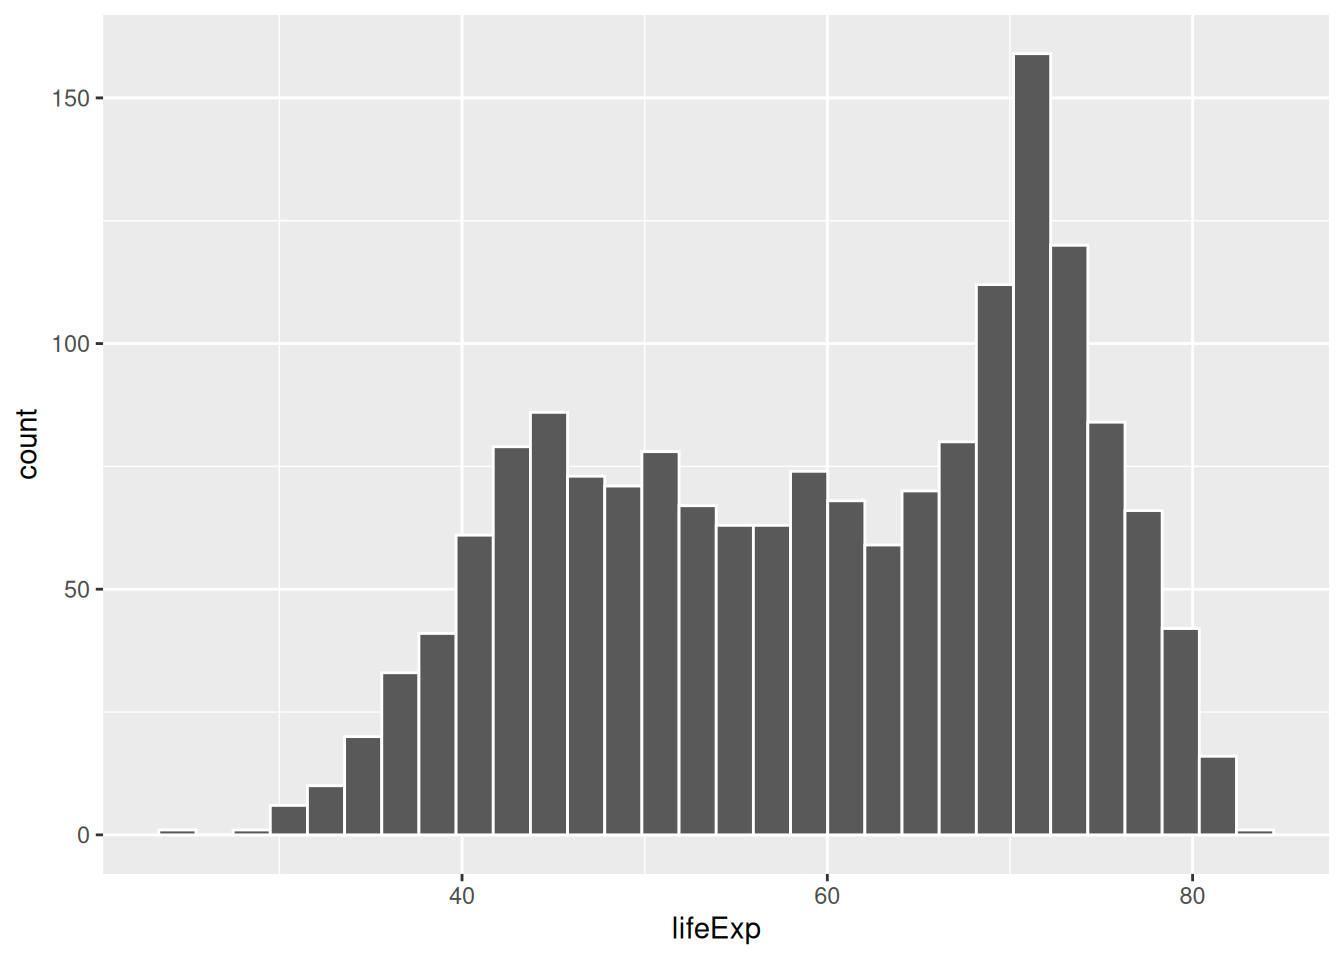
\includegraphics{Statistics_Lab_files/figure-latex/1gapminder-1.pdf}

See, that was easy. Next, is a code block that adds more layers and settings if you wanted to modify parts of the graph:

\begin{Shaded}
\begin{Highlighting}[]
\FunctionTok{ggplot}\NormalTok{(gapminder\_df, }\FunctionTok{aes}\NormalTok{(}\AttributeTok{x =}\NormalTok{ lifeExp)) }\SpecialCharTok{+}
  \FunctionTok{geom\_histogram}\NormalTok{(}\AttributeTok{color=}\StringTok{"white"}\NormalTok{)}\SpecialCharTok{+} 
  \FunctionTok{theme\_classic}\NormalTok{(}\AttributeTok{base\_size =} \DecValTok{15}\NormalTok{) }\SpecialCharTok{+}
  \FunctionTok{ylab}\NormalTok{(}\StringTok{"Frequency count"}\NormalTok{) }\SpecialCharTok{+} 
  \FunctionTok{xlab}\NormalTok{(}\StringTok{"Life Expectancy"}\NormalTok{) }\SpecialCharTok{+}
  \FunctionTok{ggtitle}\NormalTok{(}\StringTok{"Histogram of Life Expectancy from Gapminder"}\NormalTok{)}
\end{Highlighting}
\end{Shaded}

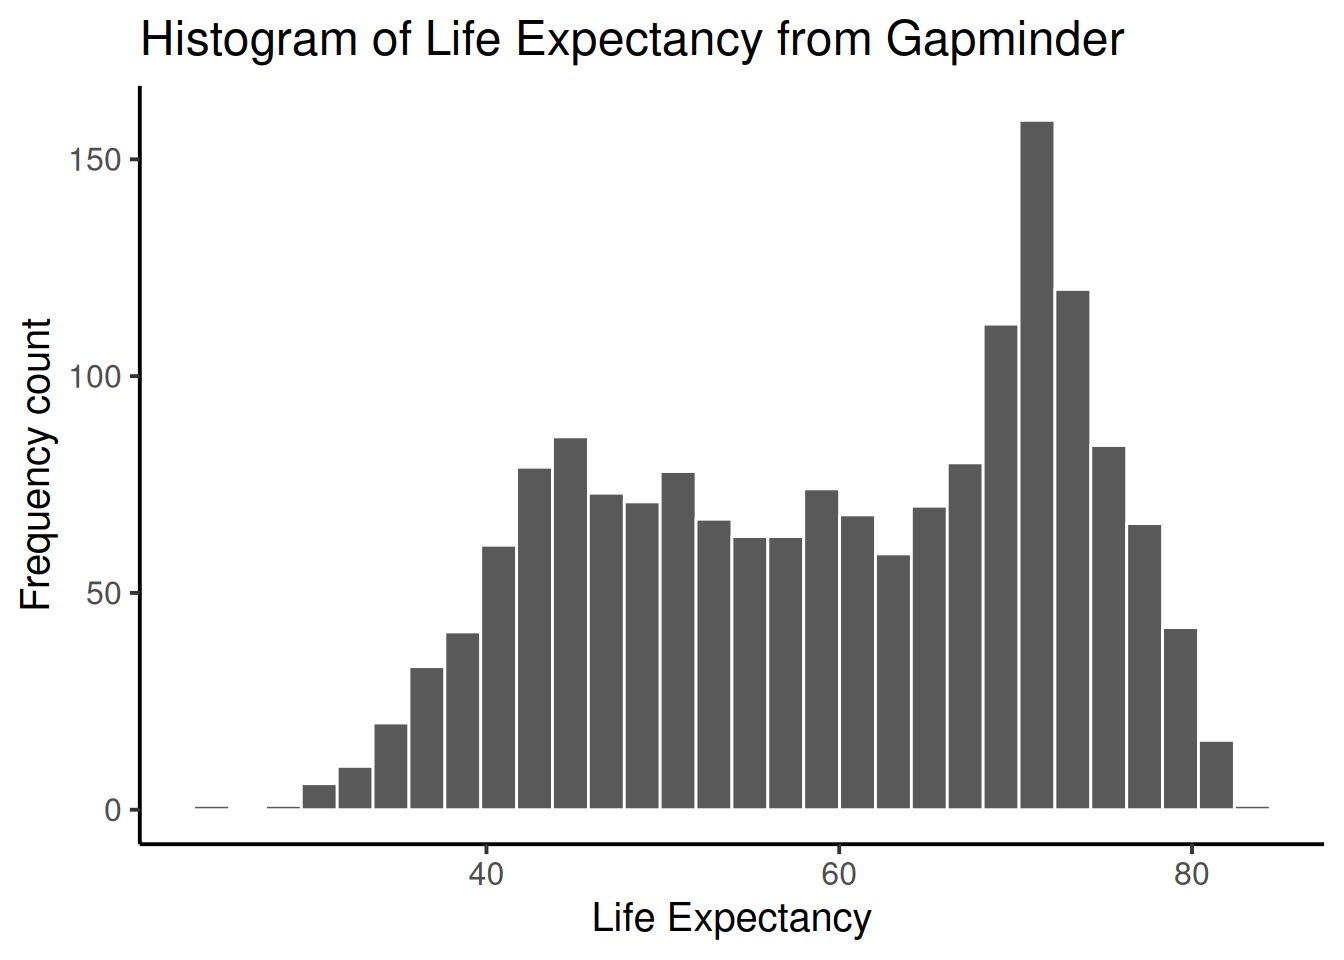
\includegraphics{Statistics_Lab_files/figure-latex/1gapminderB-1.pdf}

The histogram shows a wide range of life expectancies, from below 40 to just over 80. Histograms are useful, they can show you what kinds of values happen more often than others.

One final thing about histograms in ggplot. You may want to change the bin size. That controls how wide or narrow, or the number of bars (how they split across the range), in the histogram. You need to set the \texttt{bins=} option in \texttt{geom\_histogram()}.

\begin{Shaded}
\begin{Highlighting}[]
\FunctionTok{ggplot}\NormalTok{(gapminder\_df, }\FunctionTok{aes}\NormalTok{(}\AttributeTok{x =}\NormalTok{ lifeExp)) }\SpecialCharTok{+}
  \FunctionTok{geom\_histogram}\NormalTok{(}\AttributeTok{color=}\StringTok{"white"}\NormalTok{, }\AttributeTok{bins=}\DecValTok{50}\NormalTok{)}\SpecialCharTok{+} 
  \FunctionTok{theme\_classic}\NormalTok{(}\AttributeTok{base\_size =} \DecValTok{15}\NormalTok{) }\SpecialCharTok{+}
  \FunctionTok{ylab}\NormalTok{(}\StringTok{"Frequency count"}\NormalTok{) }\SpecialCharTok{+} 
  \FunctionTok{xlab}\NormalTok{(}\StringTok{"Life Expectancy"}\NormalTok{) }\SpecialCharTok{+}
  \FunctionTok{ggtitle}\NormalTok{(}\StringTok{"Histogram of Life Expectancy from Gapminder"}\NormalTok{)}
\end{Highlighting}
\end{Shaded}

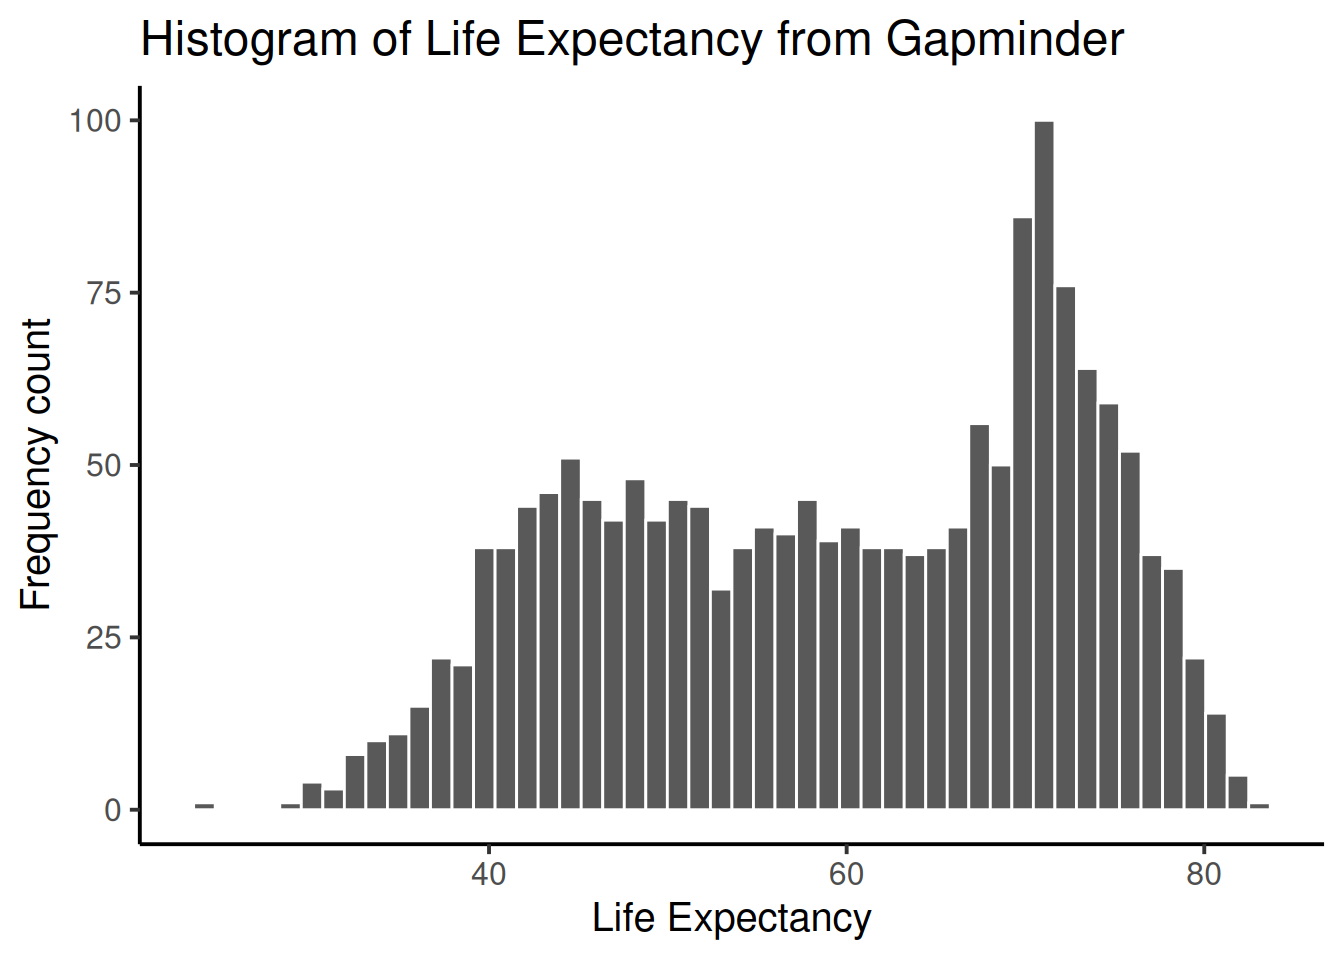
\includegraphics{Statistics_Lab_files/figure-latex/1gapminderC-1.pdf}

See, same basic patter, but now breaking up the range into 50 little equal sized bins, rather than 30, which is the default. You get to choose what you want to do.

\hypertarget{life-expectancy-by-year-scatterplot}{%
\subsubsection{Life Expectancy by year Scatterplot}\label{life-expectancy-by-year-scatterplot}}

We can see we have data for life expectancy and different years. So, does worldwide life expectancy change across the years in the data set? As we go into the future, are people living longer?

Let's look at this using a scatter plot. We can set the x-axis to be year, and the y-axis to be life expectancy. Then we can use \texttt{geom\_point()} to display a whole bunch of dots, and then look at them. Here's the simple code:

\begin{Shaded}
\begin{Highlighting}[]
\FunctionTok{ggplot}\NormalTok{(gapminder\_df, }\FunctionTok{aes}\NormalTok{(}\AttributeTok{y=}\NormalTok{ lifeExp, }\AttributeTok{x=}\NormalTok{ year))}\SpecialCharTok{+}
  \FunctionTok{geom\_point}\NormalTok{()}
\end{Highlighting}
\end{Shaded}

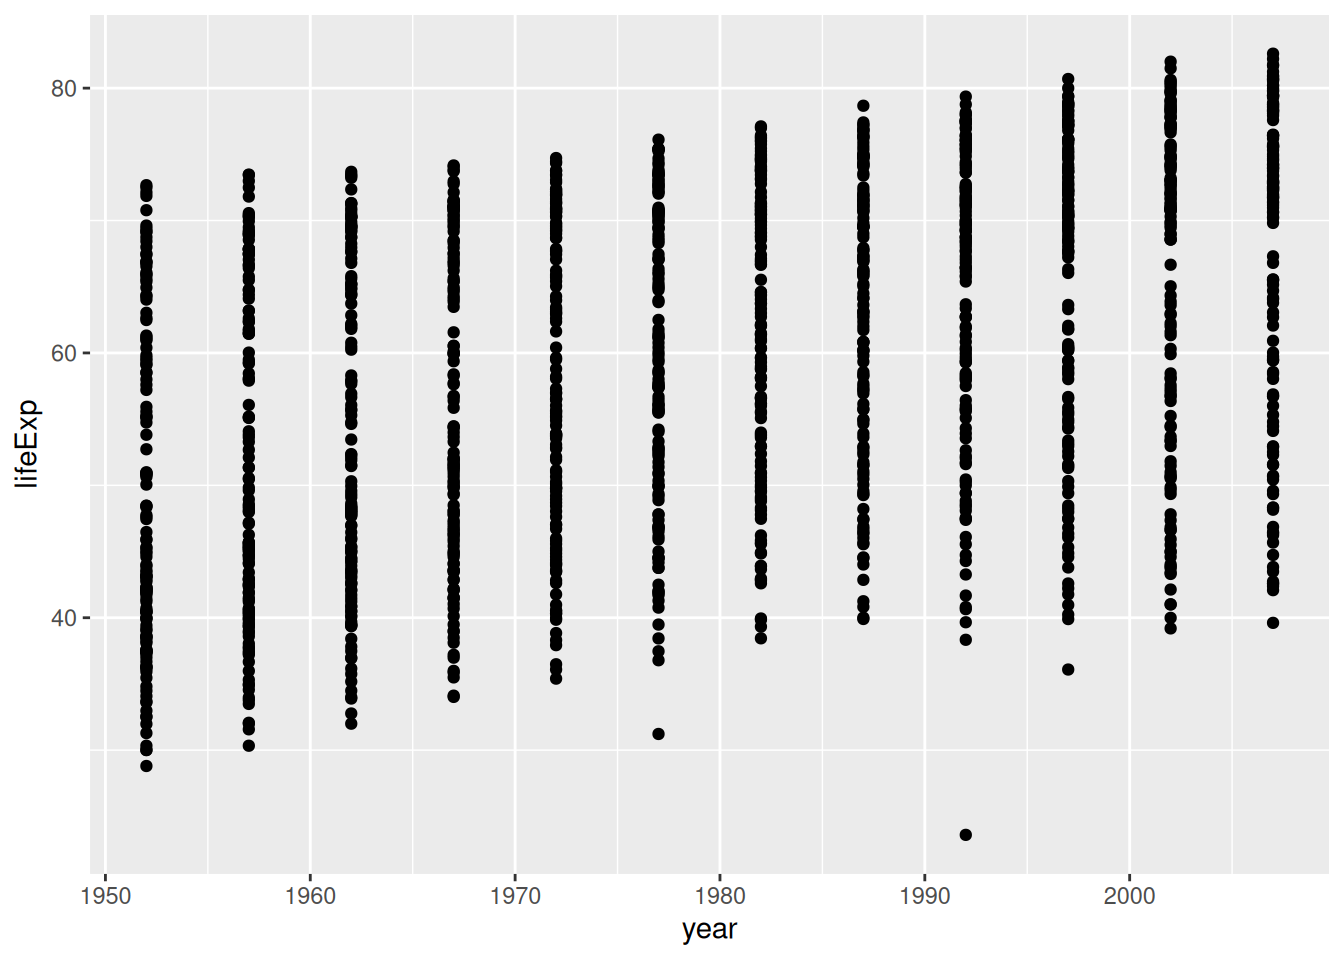
\includegraphics{Statistics_Lab_files/figure-latex/1scatterplot-1.pdf}

Whoa, that's a lot of dots! Remember that each country is measured each year. So, the bands of dots you see, show the life expectancies for the whole range of countries within each year of the database. There is a big spread inside each year. But, on the whole it looks like groups of dots slowly go up over years.

\hypertarget{one-country-life-expectancy-by-year}{%
\subsubsection{One country, life expectancy by year}\label{one-country-life-expectancy-by-year}}

I'm (Matt) from Canada, so maybe I want to know if life expectancy for Canadians is going up over the years. To find out the answer for one country, we first need to split the full data set, into another smaller data set that only contains data for Canada. In other words, we want only the rows where the word ``Canada'' is found in the \texttt{country} column. We will use the \texttt{filter} function from \texttt{dplyr} for this:

\begin{Shaded}
\begin{Highlighting}[]
\CommentTok{\# filter rows to contain Canada}

\NormalTok{smaller\_df }\OtherTok{\textless{}{-}}\NormalTok{ gapminder\_df }\SpecialCharTok{\%\textgreater{}\%} 
                 \FunctionTok{filter}\NormalTok{(country }\SpecialCharTok{==} \StringTok{"Canada"}\NormalTok{)}

\CommentTok{\# plot the new data contained in smaller\_df}

\FunctionTok{ggplot}\NormalTok{(smaller\_df, }\FunctionTok{aes}\NormalTok{(}\AttributeTok{y=}\NormalTok{ lifeExp, }\AttributeTok{x=}\NormalTok{ year))}\SpecialCharTok{+}
  \FunctionTok{geom\_point}\NormalTok{()}
\end{Highlighting}
\end{Shaded}

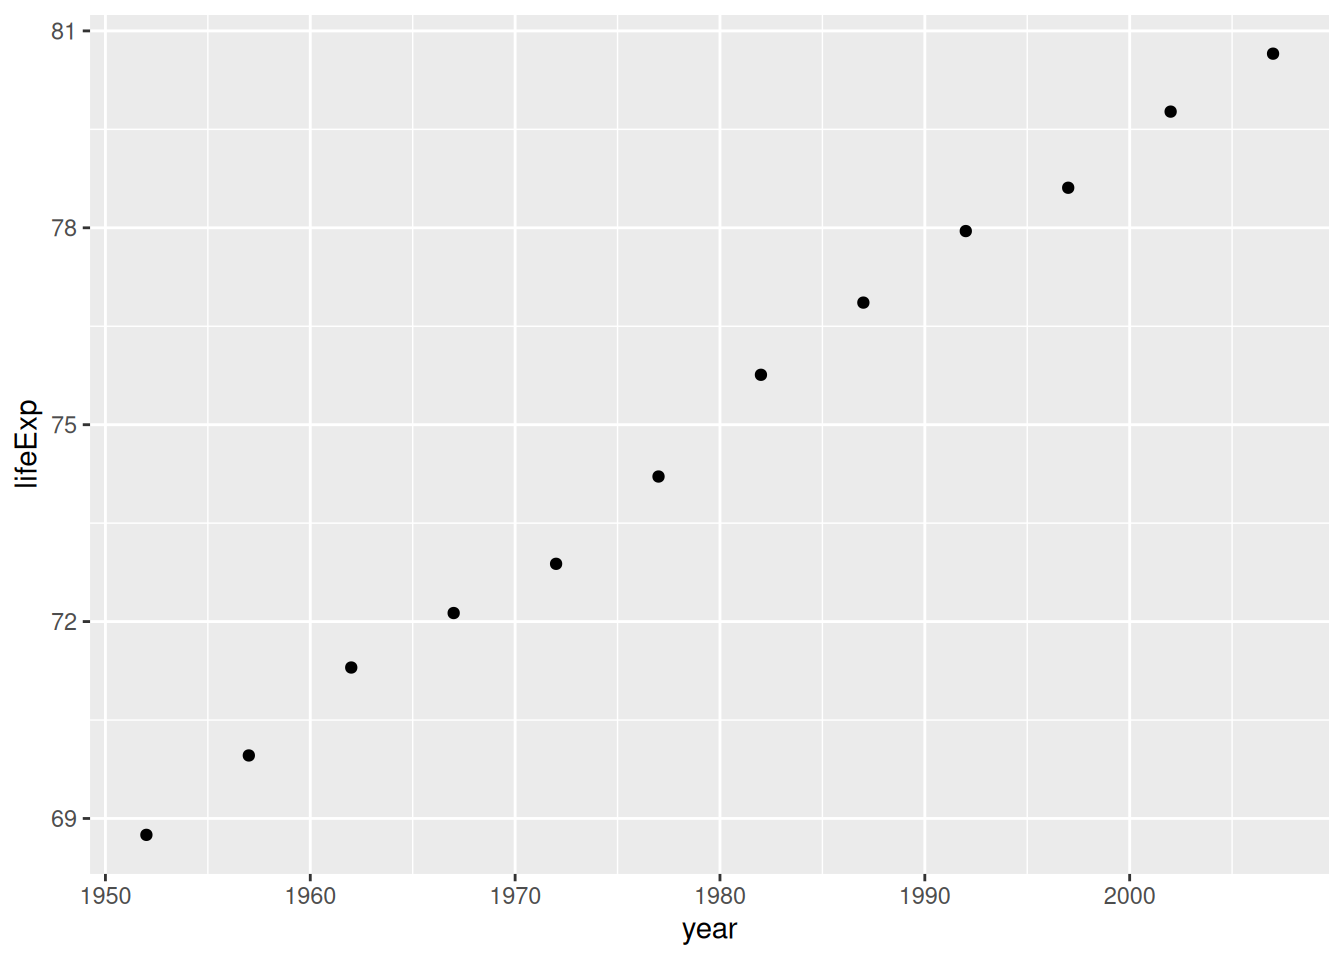
\includegraphics{Statistics_Lab_files/figure-latex/1scatterB-1.pdf}

I would say things are looking good for Canadians, their life expectancy is going up over the years!

\hypertarget{multiple-countries-scatterplot}{%
\subsubsection{Multiple countries scatterplot}\label{multiple-countries-scatterplot}}

What if we want to look at a few countries altogether. We can do this too. We just change how we filter the data so more than one country is allowed, then we plot the data. We will also add some nicer color options and make the plot look pretty. First, the simple code:

\begin{Shaded}
\begin{Highlighting}[]
\CommentTok{\# filter rows to contain countries of choice}

\NormalTok{smaller\_df }\OtherTok{\textless{}{-}}\NormalTok{ gapminder\_df }\SpecialCharTok{\%\textgreater{}\%} 
                 \FunctionTok{filter}\NormalTok{(country }\SpecialCharTok{\%in\%} \FunctionTok{c}\NormalTok{(}\StringTok{"Canada"}\NormalTok{,}\StringTok{"France"}\NormalTok{,}\StringTok{"Brazil"}\NormalTok{) }\SpecialCharTok{==} \ConstantTok{TRUE}\NormalTok{)}

\CommentTok{\# plot the new data contained in smaller\_df}

\FunctionTok{ggplot}\NormalTok{(smaller\_df, }\FunctionTok{aes}\NormalTok{(}\AttributeTok{y=}\NormalTok{ lifeExp, }\AttributeTok{x=}\NormalTok{ year, }\AttributeTok{group=}\NormalTok{ country))}\SpecialCharTok{+}
  \FunctionTok{geom\_point}\NormalTok{()}
\end{Highlighting}
\end{Shaded}

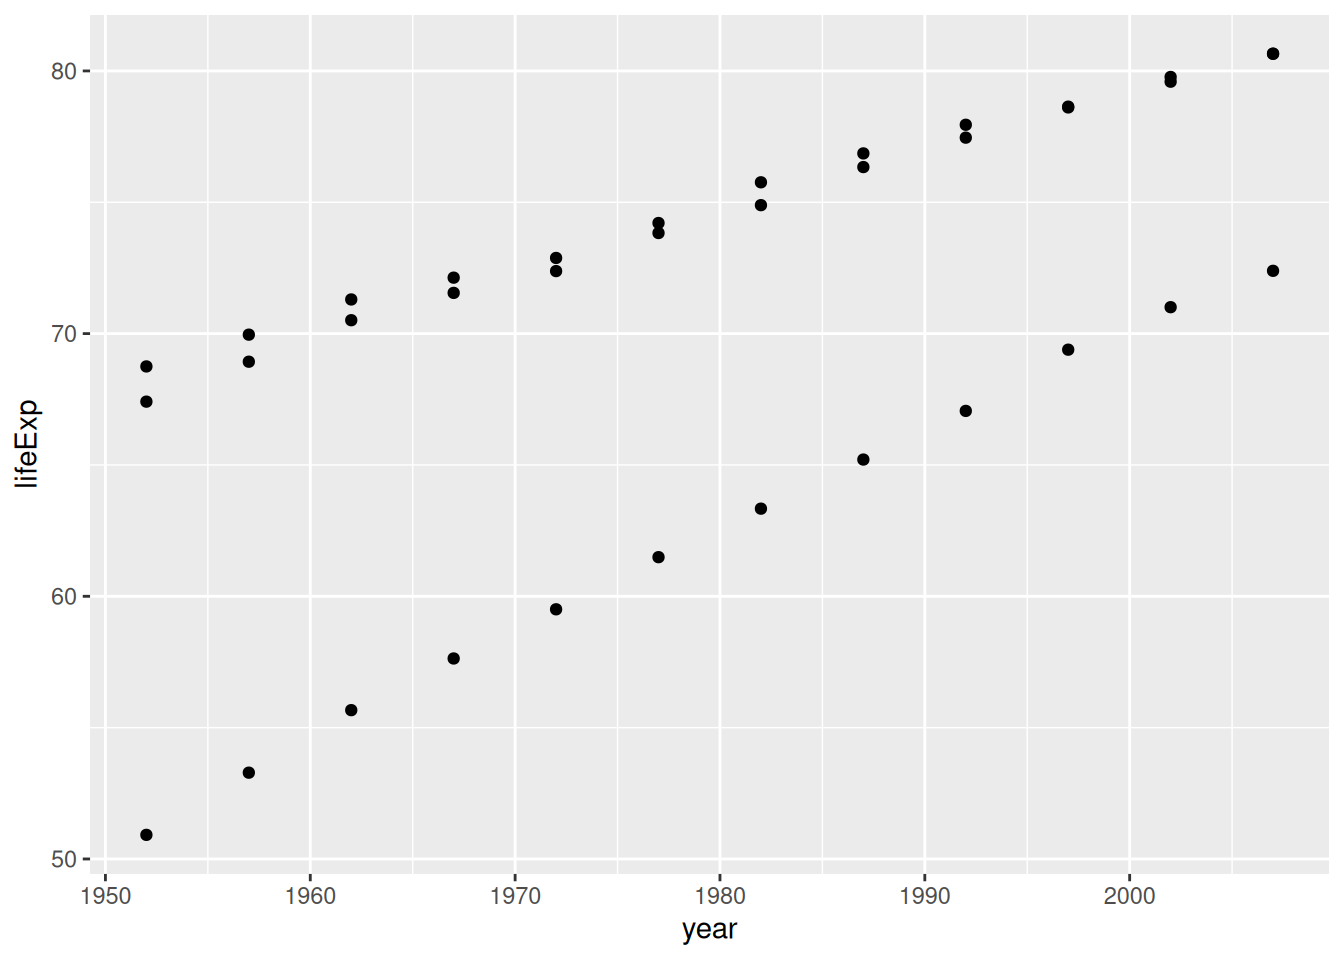
\includegraphics{Statistics_Lab_files/figure-latex/1scatterC-1.pdf}

Nice, we can now see three sets of dots, but which are countries do they represent? Let's add a legend, and make the graph better looking.

\begin{Shaded}
\begin{Highlighting}[]
\FunctionTok{ggplot}\NormalTok{(smaller\_df,}\FunctionTok{aes}\NormalTok{(}\AttributeTok{y=}\NormalTok{ lifeExp, }\AttributeTok{x=}\NormalTok{ year, }
                      \AttributeTok{group=}\NormalTok{ country, }\AttributeTok{color =}\NormalTok{ country)) }\SpecialCharTok{+}
  \FunctionTok{geom\_point}\NormalTok{()}\SpecialCharTok{+} 
  \FunctionTok{theme\_classic}\NormalTok{(}\AttributeTok{base\_size =} \DecValTok{15}\NormalTok{) }\SpecialCharTok{+}
  \FunctionTok{ylab}\NormalTok{(}\StringTok{"Life Expectancy"}\NormalTok{) }\SpecialCharTok{+} 
  \FunctionTok{xlab}\NormalTok{(}\StringTok{"Year"}\NormalTok{) }\SpecialCharTok{+}
  \FunctionTok{ggtitle}\NormalTok{(}\StringTok{"Life expectancy by year for three countries"}\NormalTok{)}
\end{Highlighting}
\end{Shaded}

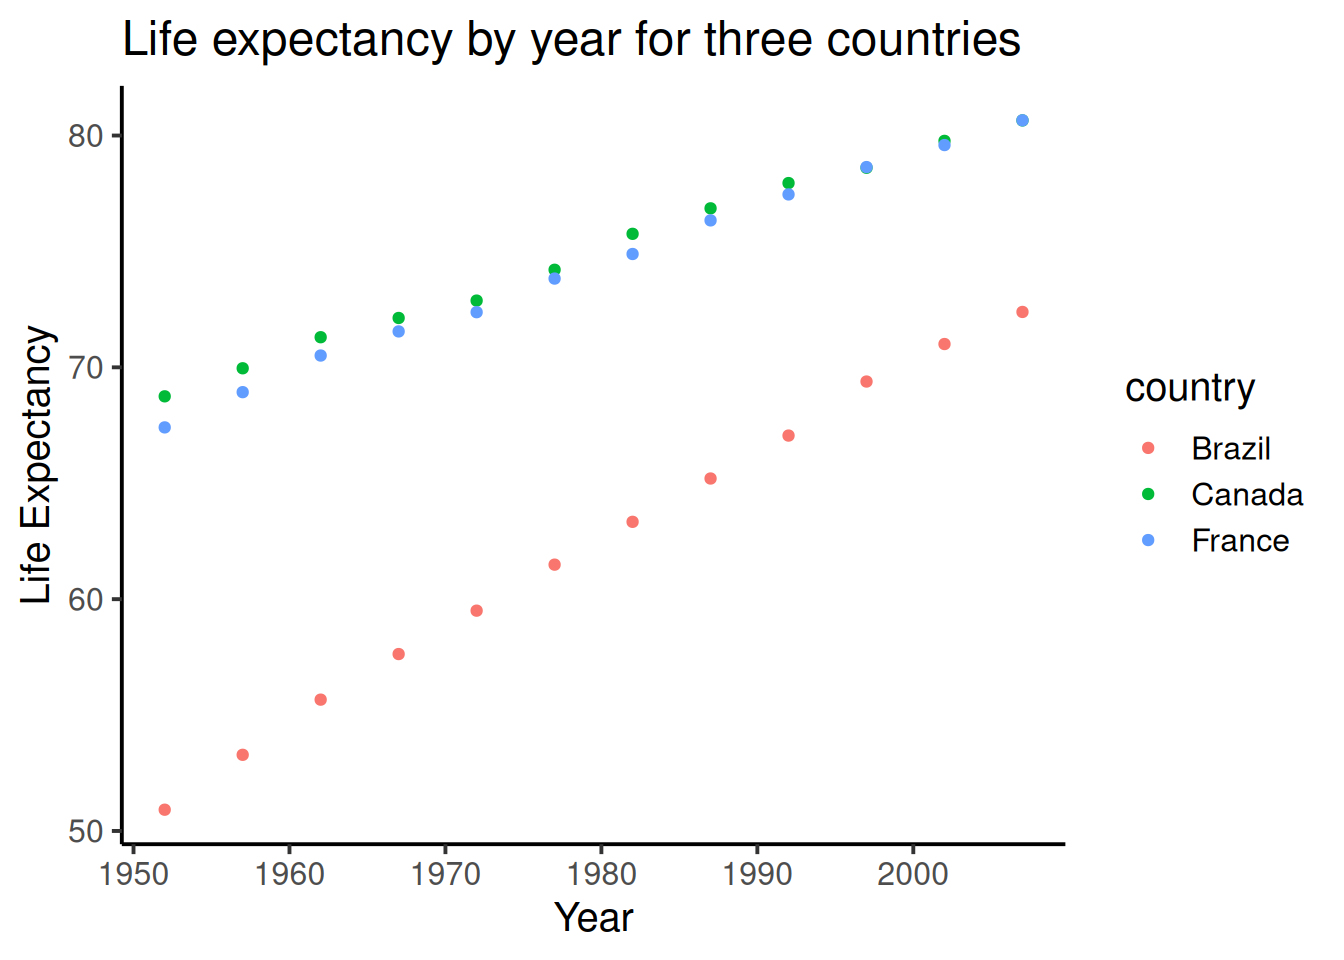
\includegraphics{Statistics_Lab_files/figure-latex/1scatterD-1.pdf}

\hypertarget{geom_line-connecting-the-dots}{%
\subsubsection{geom\_line() connecting the dots}\label{geom_line-connecting-the-dots}}

We might also want to connect the dots with a line, to make it easier to see the connection! Remember, ggplot2 draws layers on top of layers. So, we add in a new \texttt{geom\_line()} layer.

\begin{Shaded}
\begin{Highlighting}[]
\FunctionTok{ggplot}\NormalTok{(smaller\_df,}\FunctionTok{aes}\NormalTok{(}\AttributeTok{y=}\NormalTok{ lifeExp, }\AttributeTok{x=}\NormalTok{ year, }
                      \AttributeTok{group=}\NormalTok{ country, }\AttributeTok{color =}\NormalTok{ country)) }\SpecialCharTok{+}
  \FunctionTok{geom\_point}\NormalTok{()}\SpecialCharTok{+} 
  \FunctionTok{geom\_line}\NormalTok{()}\SpecialCharTok{+}
  \FunctionTok{theme\_classic}\NormalTok{(}\AttributeTok{base\_size =} \DecValTok{15}\NormalTok{) }\SpecialCharTok{+}
  \FunctionTok{ylab}\NormalTok{(}\StringTok{"Life Expectancy"}\NormalTok{) }\SpecialCharTok{+} 
  \FunctionTok{xlab}\NormalTok{(}\StringTok{"Year"}\NormalTok{) }\SpecialCharTok{+}
  \FunctionTok{ggtitle}\NormalTok{(}\StringTok{"Life expectancy by year for three countries"}\NormalTok{)}
\end{Highlighting}
\end{Shaded}

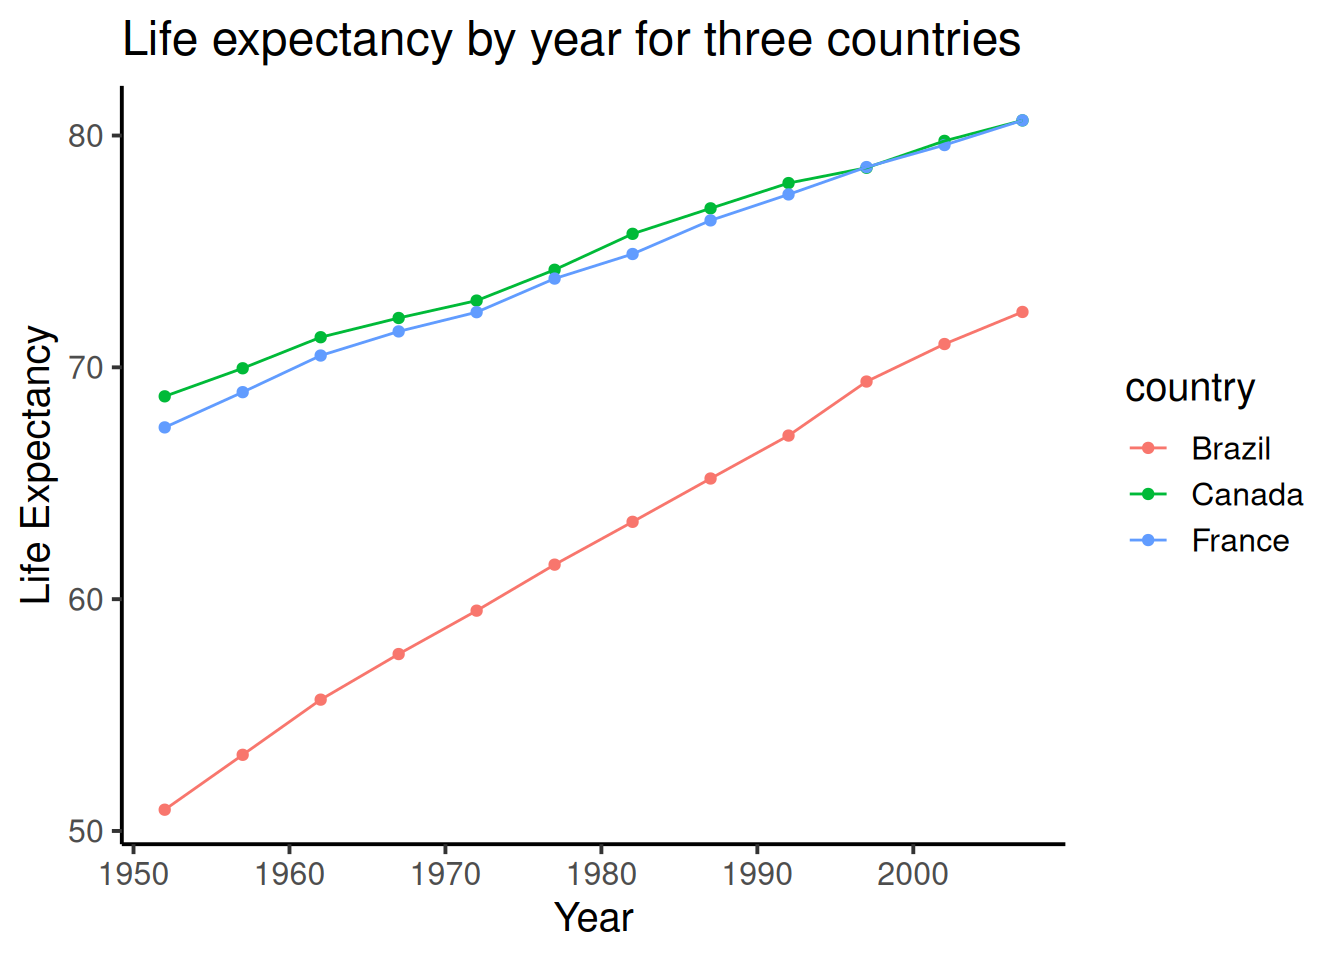
\includegraphics{Statistics_Lab_files/figure-latex/1scatline-1.pdf}

\hypertarget{generalization-exercise}{%
\subsection{Generalization Exercise}\label{generalization-exercise}}

The following generalization exercise and writing assignment is also in your lab R Markdown document for this lab. Complete your work in that document and hand it in.

(1 point - Pass/Fail)

Use the code from above to attempt to solve the extra things we ask you do for this assignment. You generalization exercises are as follows:

\begin{enumerate}
\def\labelenumi{\arabic{enumi}.}
\item
  Make a graph plotting Life Expectancy by year for the five continents, using the \texttt{continent} factor. Make sure you change the title so it reads correctly
\item
  Make a graph plotting GDP per capita by year for the USA, Canada, and Mexico. Use the \texttt{gdpPercap} column for the GDP per capita data
\item
  Make a new graph plotting anything you are interested in using the gapminder dataset. It just needs to be a plot that we have not given an example for
\end{enumerate}

\hypertarget{writing-assignment}{%
\subsection{Writing assignment}\label{writing-assignment}}

Complete the writing assignment described in your R Markdown document for this lab. When you have finished everything. Knit the document and hand in your stuff (you can submit your .RMD file to blackboard if it does not knit.)

The question for this lab is a long answer question about histograms. Here is the question:

Describe what histograms are, how to interpret them, and what they are useful for. You should answer each of these questions:

The answers to each of these questions are worth .25 points each, for a total of 2 points

\begin{enumerate}
\def\labelenumi{\alph{enumi}.}
\tightlist
\item
  What do the bars on a histogram represent?
\item
  How many bars can a histogram have?
\item
  What do the heights of the bars tell you
\item
  What is on the x-axis and y-axis of a histogram
\item
  What does the tallest bar on a histogram tell you?
\item
  What does the shortest bar on a histogram tell you?
\item
  What are some uses for histograms, why would you want to look at a histogram of some numbers that you collected?
\item
  Imagine you had two histograms, one was very wide and spread out, the other was very narrow with a very tall peak. Which histogram would you expect to contain more consistent numbers (numbers that are close to each other), explain why.
\end{enumerate}

\textbf{Rubric}

General grading.

\begin{itemize}
\tightlist
\item
  You will receive 0 points for missing answers (say, if you do not answer question c, then you will receive 0 out .25 points for that question)
\item
  You must write in complete sentences. Point form sentences will be given 0 points.
\item
  Completely incorrect answers will receive 0 points. For example, if you incorrectly describe what the x and y-axes refer to, then you will receive 0 points for that question.
\item
  If your answer is generally correct but very difficult to understand and unclear you may receive half points for the question
\end{itemize}

\hypertarget{excel-1}{%
\section{Excel}\label{excel-1}}

\hypertarget{spss-1}{%
\section{SPSS}\label{spss-1}}

In this lab, we will get you acquainted with the SPSS software layout and graph some sample data to make sense of it. We will be doing the following:

\begin{enumerate}
\def\labelenumi{\arabic{enumi}.}
\tightlist
\item
  Opening SPSS and the SPSS layout
\item
  Reviewing variable properties and the Variable View tab
\item
  Opening a data file and producing different types of graphs
\end{enumerate}

\hypertarget{opening-spss-and-the-spss-layout}{%
\subsection{Opening SPSS and the SPSS layout}\label{opening-spss-and-the-spss-layout}}

\begin{center}\rule{0.5\linewidth}{0.5pt}\end{center}

Your lab instructor will take you through the process of opening the SPSS program. You may double-click on its icon located on the desktop of your lab computer, or you may find it using the Start menu. Once the program loads, you will be prompted with a pop-up window that asks you which file you would like to open. For now, we will be examining the basic layout of SPSS without a data set, so you can click {Cancel}.

Once you do, the main SPSS spreadsheet should open. It will look like this, a basic spreadsheet:

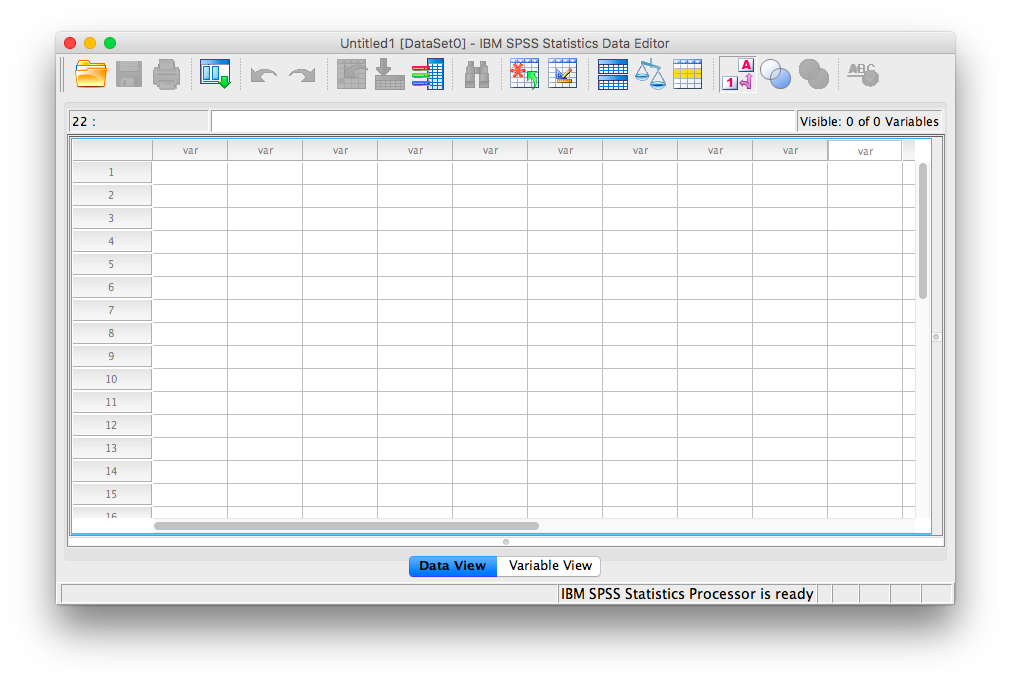
\includegraphics{img/1.4.11.png}
Notice at the bottom of your window there are two tabs; ``Data View'' and ``Variable View''. In data view, we enter data into our spreadsheet. You will notice that rows are numbered on the left-hand side of the spreadsheet, while columns are labeled ``var''. This is an indication of the general structure of SPSS: Variables are contained in the columns, and rows indicate individual observations. For example, if you obtained the heights (in inches) of 5 people \{x= 64, 70, 63, 62, 65\} and wanted to enter their data into SPSS, each person's height would be entered in a new row, not across the columns, as seen below:

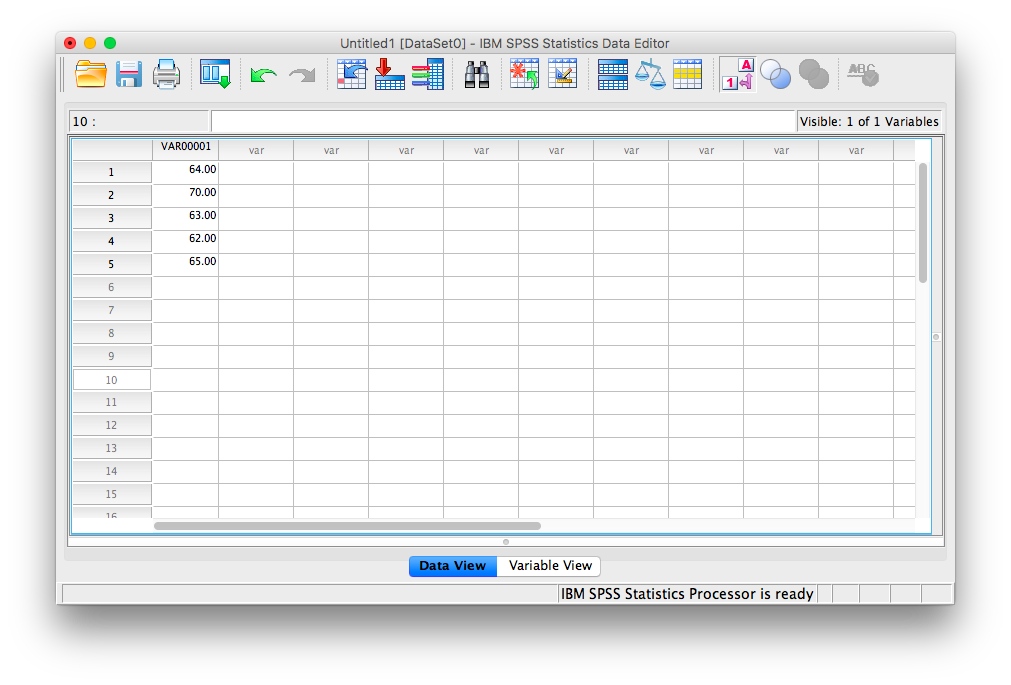
\includegraphics{img/1.4.12.png}

\hypertarget{reviewing-variable-properties-and-the-variable-view-tab}{%
\subsection{Reviewing variable properties and the Variable View tab}\label{reviewing-variable-properties-and-the-variable-view-tab}}

\begin{center}\rule{0.5\linewidth}{0.5pt}\end{center}

Now that we have some data entered, we might want to name our variable so that it's evident our measurements represent heights. In order o view or modify variable names and other properties, look to the bottom of your SPSS window and switch over to the ``Data View'' tab. Once you do this, your window will appear as follows:

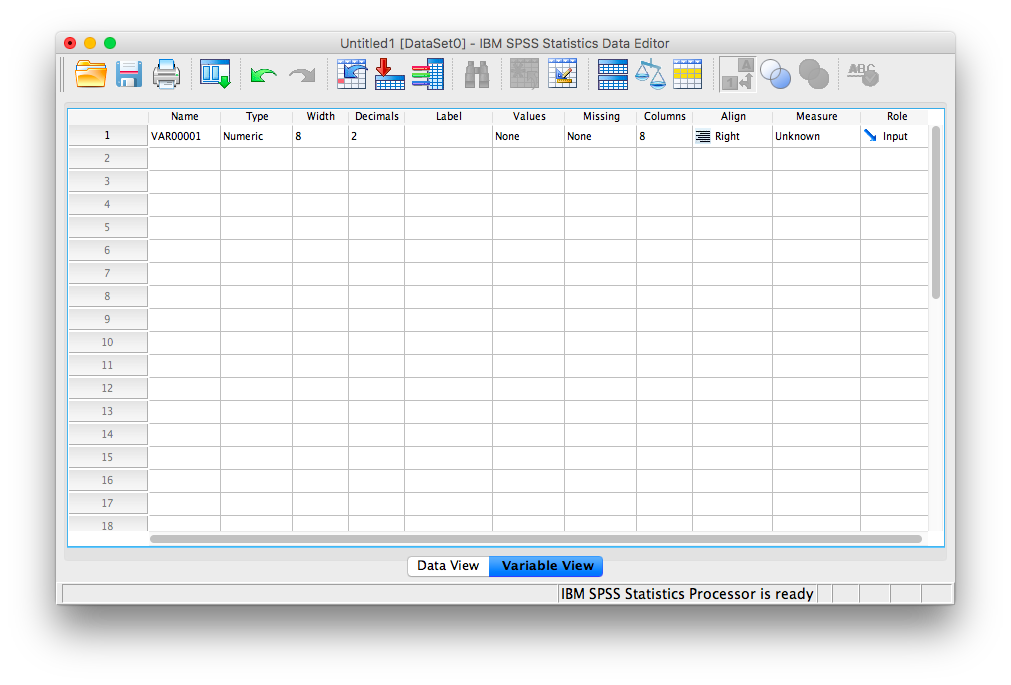
\includegraphics{img/1.4.13.png}

Here, you can edit the name of your variables, and specify their properties. Variable names can be anything you like, with the restriction that you cannot use numbers or spaces. Next, notice several other important properties of variables you may at some point need to set or modify:

\begin{itemize}
\tightlist
\item
  Name: the name of your variable that will appear as a colum header in Data View. No spaces or numerals.
\item
  Type: Your data will most often be Numeric, but sometimes, as in data representing currency or data in scientific notation, you may change the data type appropriately. If your data is simply a label, word, or response (such as an open-ended response to a survey question), choose ``String'': this tells SPSS not to treat this variable as a number. (Nota bene: if you select the wrong type of variable, SPSS may not be able to process your requested calculations, so always remember to check this parameter!)
\item
  Width: This refers to how many digits will be visible by default.
\item
  Decimals: This refers to how many decimal places will be visible by default.
\item
  Label: This is a description of the variable. Any information too long to be included in the variable name goes here.
\item
  Values: For nominal scale data, let's say 1 represents male and 2 represents female, this is where you include the values and their corresponding labels.
\item
  Measure: This variable property allows you to specify the nature of your data. Depending on the kind of scale you are using, you will choose a different measure type. Nominal and ordinal are chosen for nominal and ordinal scales, respectively. ``Scale'' is used when your data is measured on a ratio or interval scale. (Nota bene: this ``Measure'' designation is only a marker; it does not affect the calculations as in the ``Type'' parameter. Even if you choose the wrong icon/label for ``Measure'', SPSS will still produce the correct output)
\end{itemize}

\hypertarget{opening-a-data-file-and-producing-different-types-of-graphs}{%
\subsection{Opening a data file and producing different types of graphs}\label{opening-a-data-file-and-producing-different-types-of-graphs}}

\begin{center}\rule{0.5\linewidth}{0.5pt}\end{center}

Now that we know about the properties of the SPSS spreadsheet window, let's open a data file and learn how to make some sense of it by creating different types of graphs. \href{https://github.com/CrumpLab/statisticsLab/blob/master/data/spssdata/nyc_films.sav}{Here} is a link to an SPSS-based data file containing information about film permits (requests made by film companies to shoot TV shows and movies on location) filed in New York City. The file is named nyc\_films.sav.

Once you open the data file, browse through to familiarize yourself with the variables that are being measured. Switch over to Variable View for details of each variable.

\hypertarget{bar-graphs}{%
\subsubsection{Bar Graphs}\label{bar-graphs}}

\begin{center}\rule{0.5\linewidth}{0.5pt}\end{center}

Now, back to Data View. We will not be working with every single variable in this spreadsheet, but we'll select a few interesting ones with which to answer questions. Let's start with \texttt{borough}. Suppose we wanted to know which borough receives the most film permits (you can probably guess which one is most popular). Let's use SPSS to produce a graph to answer this question. With your data file open, go up to the top menu and choose {Graphs}, then {Legacy Dialogs}. You will see an entire list of possible graphs we can use to plot our data.

Let's think about the nature of our question: we would like to know how many permits were filed for each borough. Borough is simply a label or a name for a region, and we want to know the frequency of permits for each borough. This is a nominal scale variable and so, we will appropriately choose a BAR graph to plot it. Select {Bar\ldots{}}

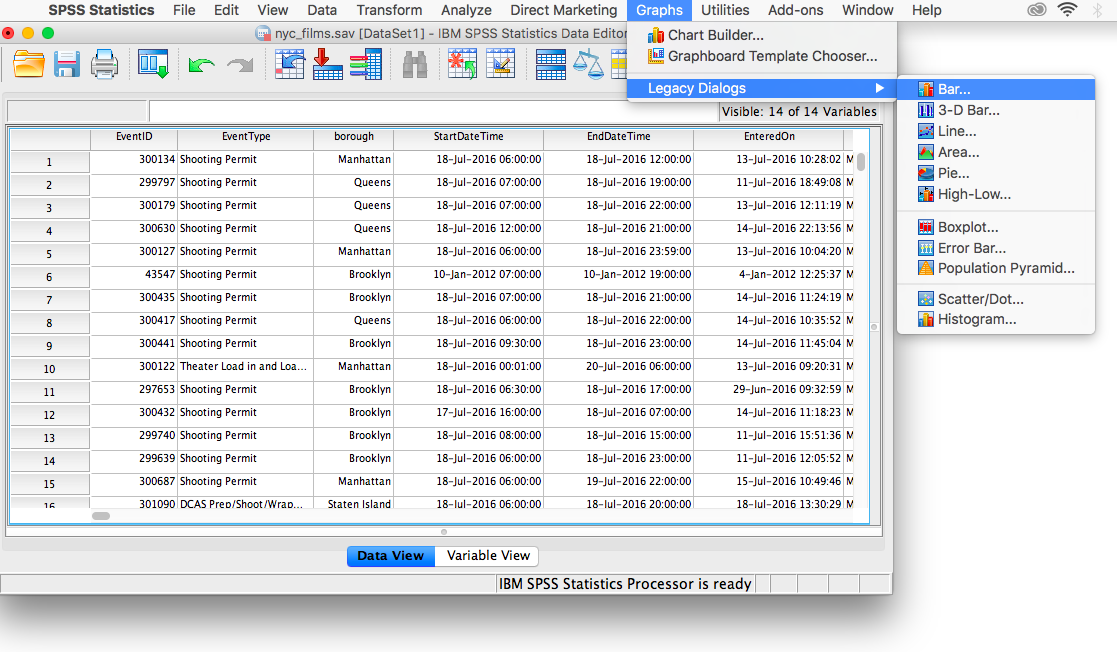
\includegraphics{img/1.4.14.png}

The next window will ask you to specify what kind of graph you would like. Select {Simple} and then {Define}.
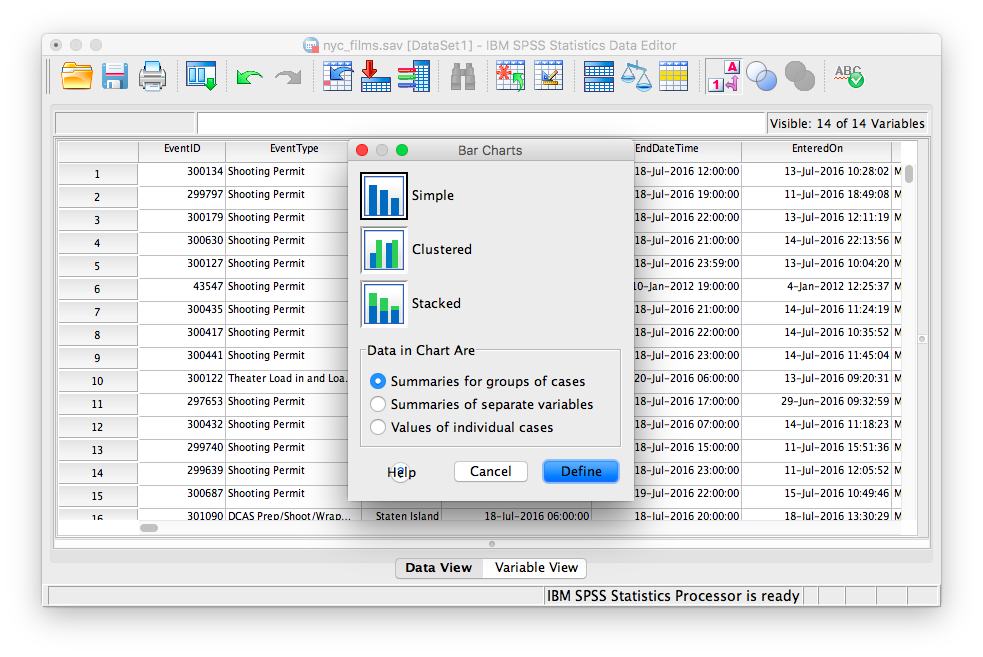
\includegraphics{img/1.4.15.png}
The following window will ask which variable you'd like to plot. Select \texttt{borough} from the left-hand list and use the arrow to move it into the field labeled ``Category Axis''. Then click {OK}.

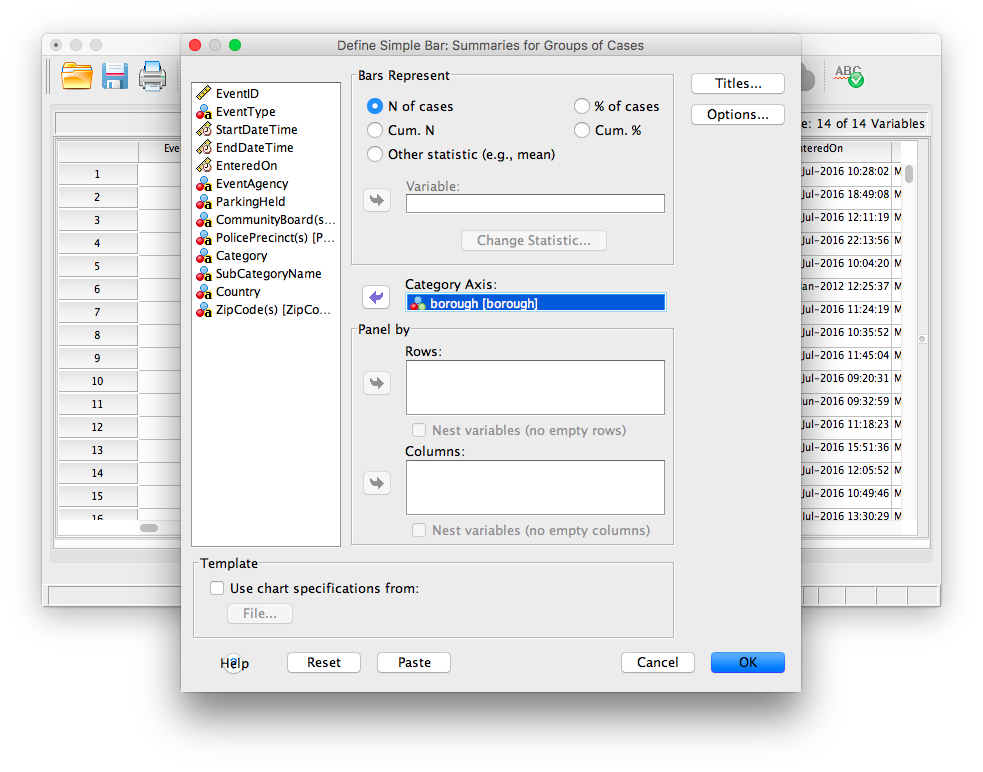
\includegraphics{img/1.4.16.png}

SPSS will produce a new output window which will contain the bar graph you have generated. Notice which borough receives the most film permits. Are you surprised?

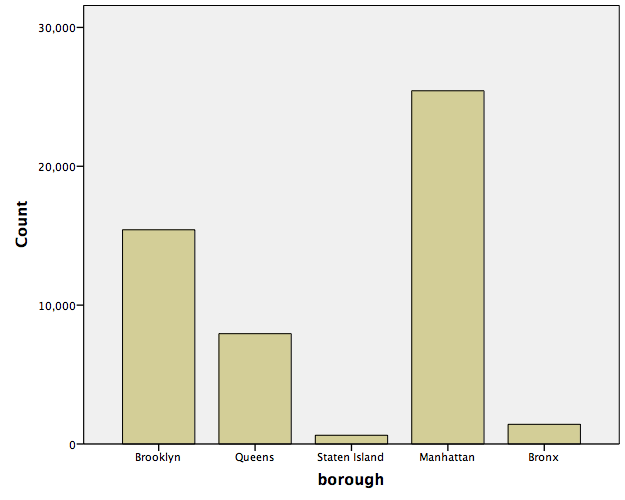
\includegraphics{img/1.4.17.png}

\hypertarget{histograms}{%
\subsubsection{Histograms}\label{histograms}}

\begin{center}\rule{0.5\linewidth}{0.5pt}\end{center}

Now, let's use a different data set to plot a histogram. The defining difference between a histogram and a bar graph (although they look very similar as they both utilize bars) is that a histogram is used to display a continuous variable (interval or ratio scale). In the previous example, boroughs were simply labels or names, so we used a nominal scale and therefore a bar graph. Here, we will deal with life expectancy (measured in years), an interval scale measure. \href{https://github.com/CrumpLab/statisticsLab/blob/master/data/spssdata/life_expectancy.sav}{Here} is a link to the SPSS data file, life\_expectancy.sav. Open this file and examine its rows and columns. Each column represents a year during which life expectancy was measured. Each row represents a different country.

Let's first get an idea about life expectancy in general. We want to plot a histogram with life expectancy on the x-axis and frequency on the y-axis. Choose {Graphs} in the top menu, then {Legacy Dialogs}. From here, remember we want a histogram, not a bar graph, so let's select {Histogram\ldots{}}.

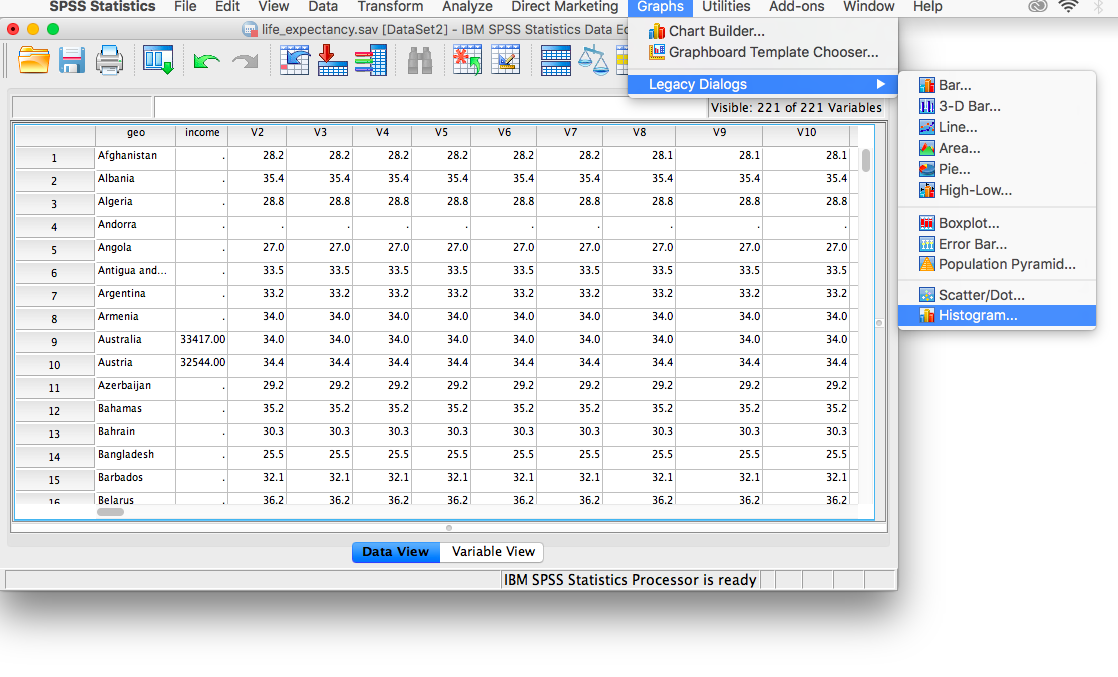
\includegraphics{img/1.4.18.png}

The window that appears contains every variable in your spreadsheet listed on the left-hand side. We can choose one variable at a time to plot. Let's scroll all the way down the list and choose \texttt{2017\ {[}v219{]}}. This is the variable containing life expectancies for the year 2017. Using the arrow, move that variable into the field labeled ``Variable:'', then click {OK}.

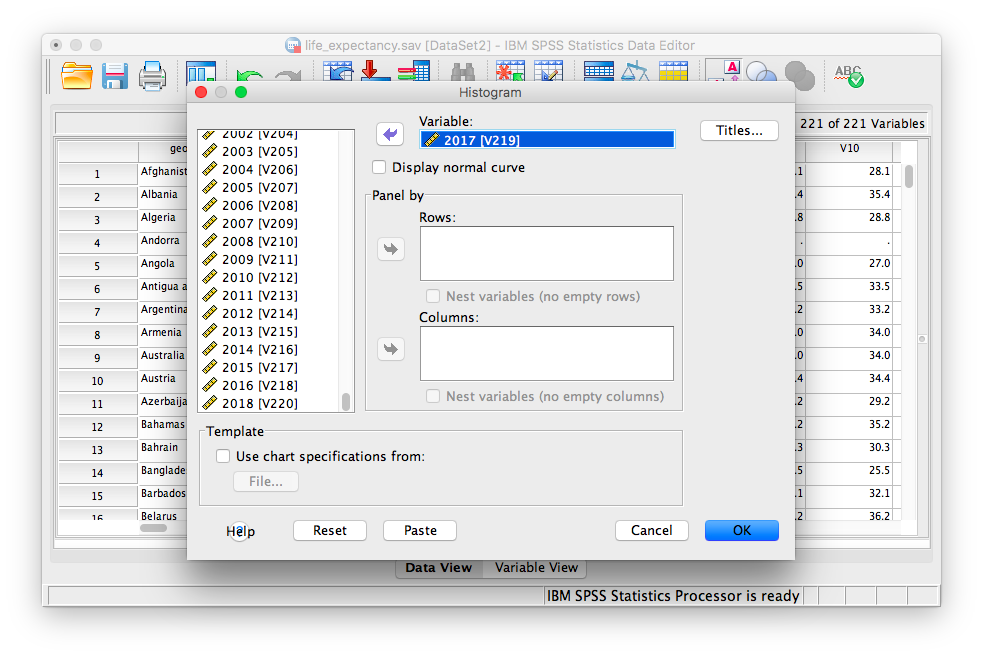
\includegraphics{img/1.4.19.png}

SPSS will produce an output window containing the distribution of life expectancy for the year 2017.

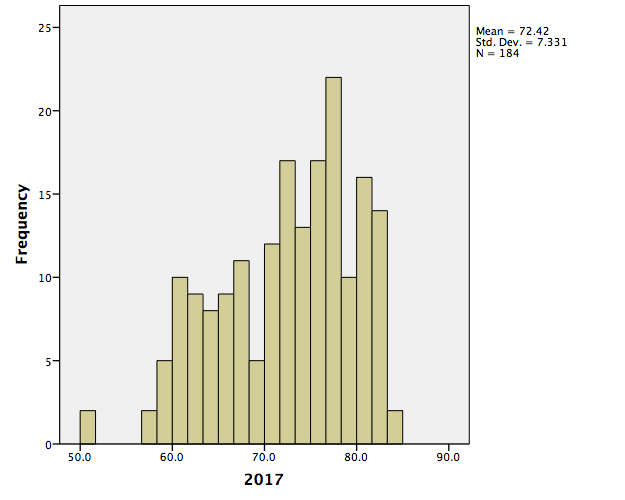
\includegraphics{img/1.4.20.png}

\hypertarget{scatterplots}{%
\subsubsection{Scatterplots}\label{scatterplots}}

\begin{center}\rule{0.5\linewidth}{0.5pt}\end{center}

Now, we will look to a different type of data plot; the scatterplot. A scatterplot allows us to visualize bivariate data, that is, data for which there are two measurements per individual. For example, we may ask whether life expectancy in a country (or how long you live, on average) is related to the average income. Using the life\_expectancy.sav data file, let's plot both variables: \texttt{2017\ {[}v219{]}} and \texttt{income}. The income variable in the spreadsheet refers to data collected in 2017 by the Better Life Initiative. Notice not all the countries listed have estimates for average annual income. For those that do, this value represents household net adjusted income (annual) in US dollars.

To create the scatterplot, let's go to {Graphs} in the menu toolbar, then {Legacy Dialogs}, then {Scatter}.

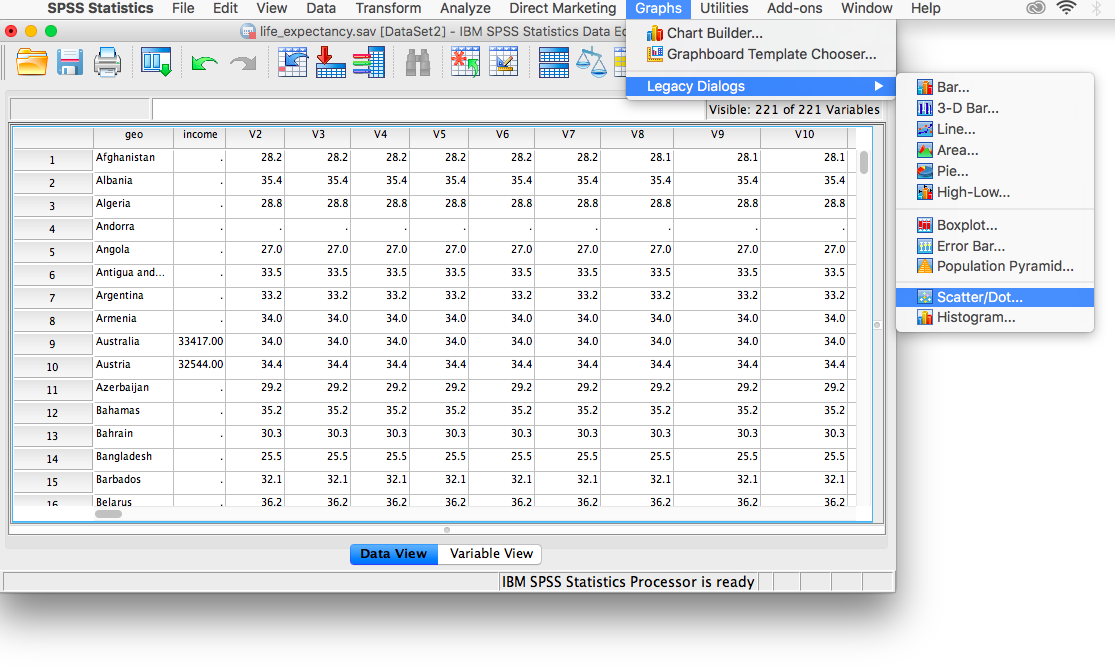
\includegraphics{img/1.4.21.png}

You will choose {Simple} scatter, then click {Define}.
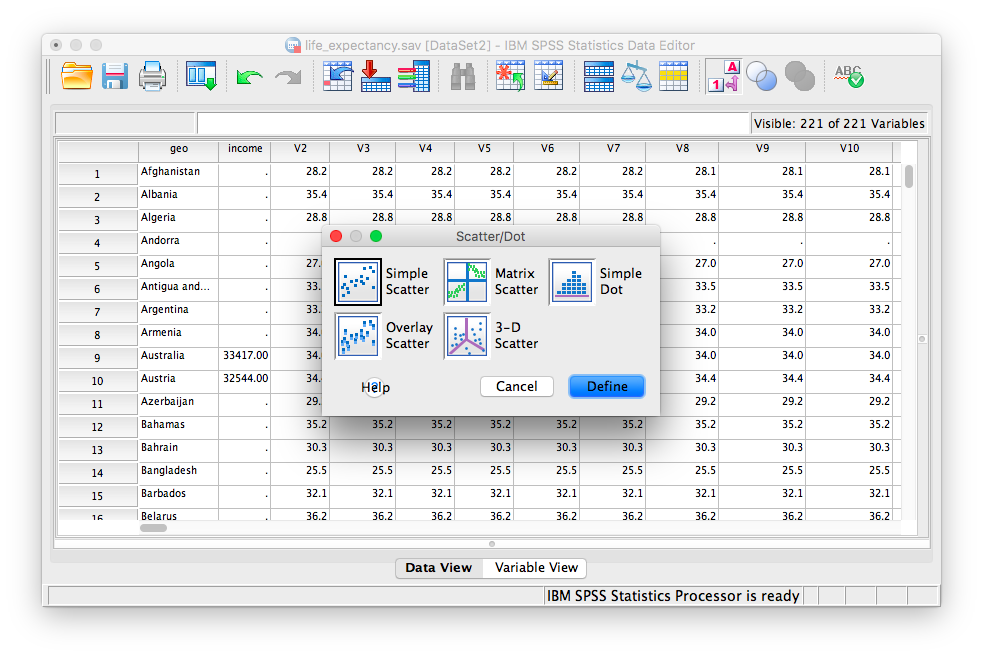
\includegraphics{img/1.4.22.png}

Next, indicate which variables (there are 2 this time!) you would like in the x- and y-axes. Use the arrows to place \texttt{income} in the x-axis field, and \texttt{2017\ (V219)} in the y-axis field. (For the purposes of graphing a scatterplot, it does not matter which variable goes into the y-axis and x-axis fields for now; you can reverse them if you'd like and you can still interpret the data similarly)

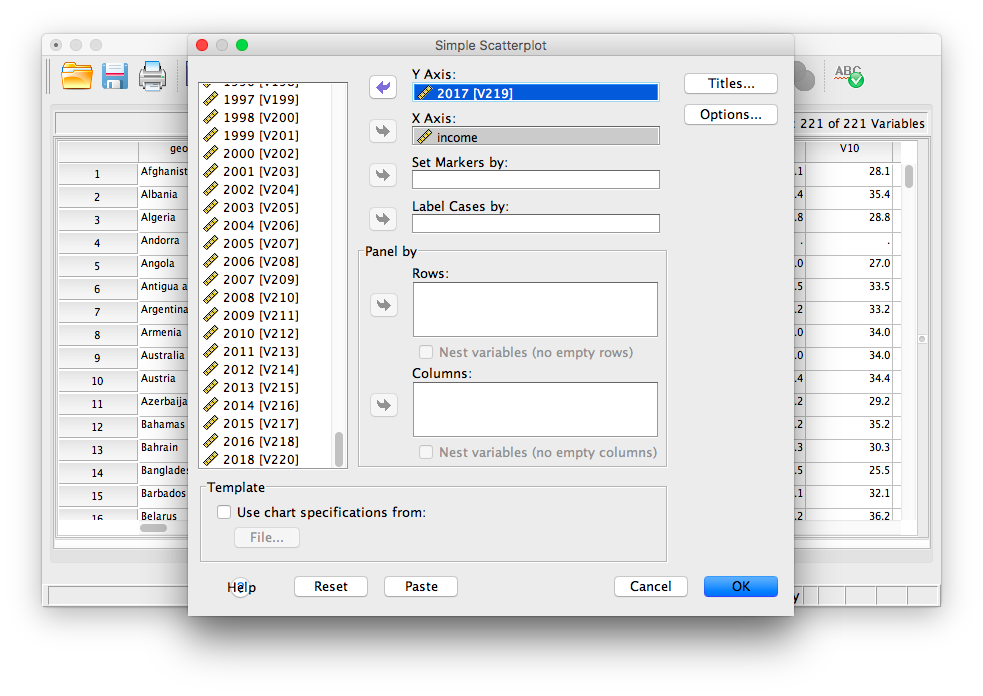
\includegraphics{img/1.4.23.png}

Then click {OK}.
SPSS will produce output containing a scatterplot. What relationship do you notice? What happens to life expectancy the more individuals earn, on average?

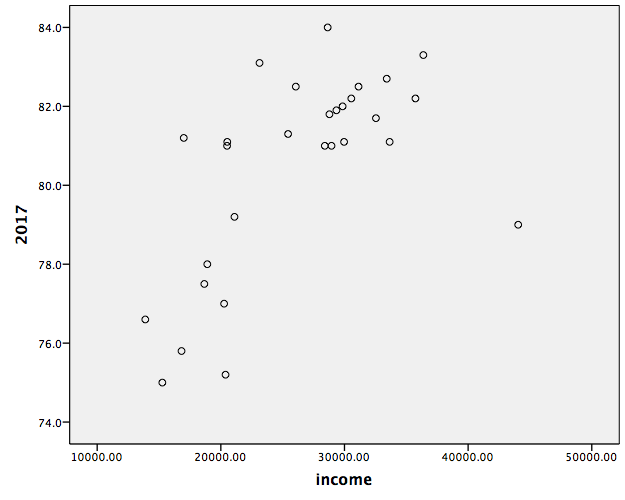
\includegraphics{img/1.4.24.png}

\hypertarget{practice-problems}{%
\subsection{Practice Problems}\label{practice-problems}}

\begin{center}\rule{0.5\linewidth}{0.5pt}\end{center}

\begin{enumerate}
\def\labelenumi{\arabic{enumi}.}
\item
  Create a histogram for life expectancy in the year 1800. Describe the distribution. How does it differ from the one we plotted for 2017?
\item
  Plot the life expectancy of each country in 1800 vs.~that of 2018. What does this graph show you? What are your conclusions regarding the development of nations?
\end{enumerate}

\hypertarget{jamovi-1}{%
\section{JAMOVI}\label{jamovi-1}}

\hypertarget{cogstat-2}{%
\section{CogStat}\label{cogstat-2}}

When we measure things, we often get so much data that it is almost impossible to manage them without any help. A simple helpful thing to do if you would like to understand your data better is to give them a graphical appearance. In this chapter, we will make charts, plots, and summaries to look at, rather than the numbers themselves. With the help of CogStat, we can graph data and get to know the descriptive statistics of our dataset.

\hypertarget{goals}{%
\subsection{Goals}\label{goals}}

\begin{itemize}
\item
  Load data into CogStat
\item
  Overview data structure
\item
  Create and understand graphs
\end{itemize}

\hypertarget{load-the-data-into-cogstat}{%
\subsection{Load the data into CogStat}\label{load-the-data-into-cogstat}}

We will start every task with the same first step, which is, to load the dataset into CogStat. In this part, we will use the dataset ``Film\_Permits'' (\url{https://opendata.cityofnewyork.us/}). As mentioned in the previous chapter, to load the data into CogStat, choose ``Data'', then ``Open demo data File\ldots{}''. It is also possible to drag and drop the file or copy and paste it to the CogStat window. After loading the dataset, you will see the following things, as displayed in the picture above:

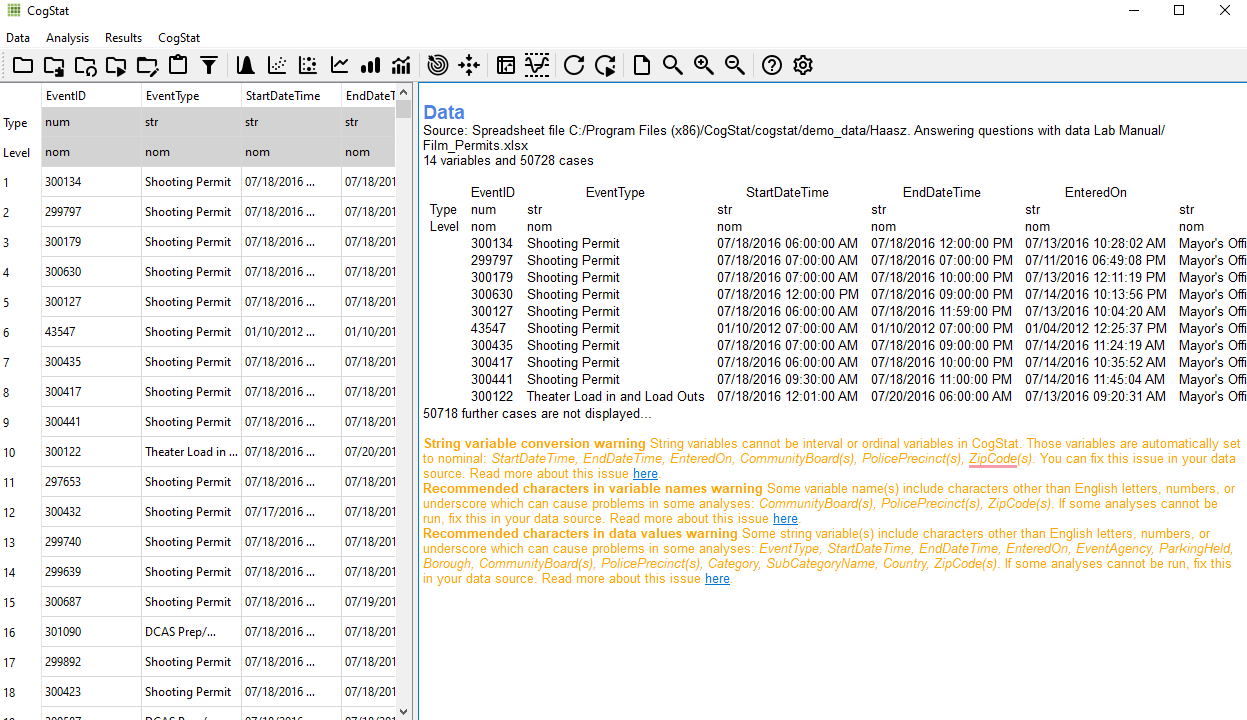
\includegraphics{img/ch1/CS_homepage.png}

In CogStat, as you can see in the picture above, there are two separate areas or panes: on the left, we have all our variables and data, and the right side functions as an output, where the results of our tests will appear.

\hypertarget{warnings-and-error-messages}{%
\subsection{Warnings and error messages}\label{warnings-and-error-messages}}

There might be cases, like the one in the picture above, when you will see some warning or error messages.
``String variable conversion warning'' and ``Measurement level warning'': As in many other statistical software, in CogStat variables can be set to nominal, ordinal, or interval (Ratio data is also handled as interval). Since automatic data processing relies on measurement levels a lot, to decide what test to run on the variables, it is important to set the variable measurement levels beforehand. As you can see in the message, string variables are handled as nominal in CogStat.
Also, it is always useful and recommended to use short variable names with English characters only. (for more: \url{https://doc.cogstat.org/Handling-data})

You might see error messages that are not related to your imported data, for example, a message like ``Oops, something went wrong.'' will be sent by CogStat if an analysis cannot be completed because of a software error. Depending on your preferences, you can ask CogStat to give you detailed error messages related to these types of error messages. To change these settings select the option ``Preferences'' (Ctrl+Shift+P) and pick ``On'' or ``Off'' at ``Detailed error message''. Turning the detailed error messages on can help if you find a bug and would like to report it to us, as with bug reports we always ask for detailed error messages.
If you would like to get more information on how to report a bug visit the following link: \url{https://doc.cogstat.org/Report-a-bug}

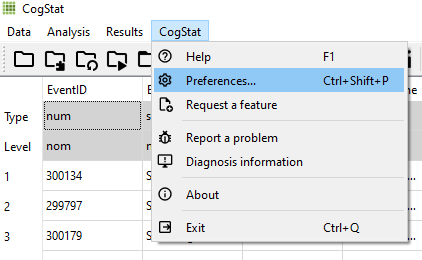
\includegraphics{img/ch1/preferences.png}

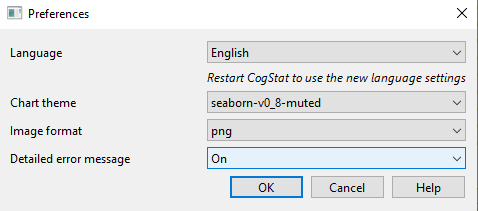
\includegraphics{img/ch1/detailederror.png}

\hypertarget{where-are-the-most-film-permits-being-requested-1}{%
\subsection{Where are the most film permits being requested?}\label{where-are-the-most-film-permits-being-requested-1}}

If we look at the dataset we loaded into CogStat previously, it shows us that 50,728 film permits were made. Different columns tell us information about each of the film permits. For example, the Borough column lists the Borough for each request, whether it was made for Manhattan, Brooklyn, Bronx, Queen's, or Staten Island. Now we can ask our first question, and learn how to plot in CogStat. First, we would like to know where the most film permits were requested.

Do you have any guesses? Is it Manhattan, Brooklyn, Queen's, or Staten Island? We might have a guess, but among this large pile of data, it will probably be wrong, and guessing is not scientific. We can find the answer by plotting the data, using a bar plot. We just need to count how many film permits are requested in each borough, and then make different bars to represent the counts.

\hypertarget{running-your-first-analysis-explore-variable}{%
\subsubsection{Running your first analysis (Explore variable)}\label{running-your-first-analysis-explore-variable}}

To do that, return to our dataset, and select the ``Explore variable'' analysis (Ctrl+1). You can choose it from the Quick Access Toolbar or the ``Analysis'' menu.

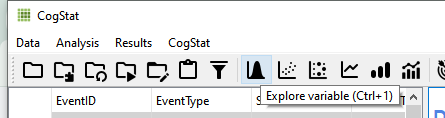
\includegraphics{img/ch1/explorevariable1.png}

or

\includegraphics{img/ch1/explorevariable2.png}

From ``Analysis'' you can find all the available analyses, to choose from. Keep in mind that there are no specific tests or graph names to choose from here, as in all cases a task can be chosen. After choosing ``Explore variable'' a dialogue appears.

\includegraphics{img/ch1/explorevariables.png}

In the dialogue, select the variable ``Borough'' and click on the arrow pointing to the right, or drag and drop the variable from ``Available variables'' to ``Selected variable(s)''. Make sure that ``frequencies'' is ticked in and press ``OK''. (Although, the ``Frequencies'' button is ticked by default.)

\hypertarget{checking-the-results-of-the-analysis}{%
\subsubsection{Checking the results of the analysis}\label{checking-the-results-of-the-analysis}}

Making the result interpretation even easier, the output's structure in almost every analysis is very similar: First, you see the raw data, then the sample properties, and finally, the population properties. (1) In the raw data section of the output, the number of observed and missing values are counted. All missing values will be excluded from further operations. To understand your data and its parameters better in every case, graphs are also provided with the raw data only. (2) In the sample properties, descriptive statistics are included, with standardised effect sizes, and summaries with graphs. (3) Population properties come with estimations about the population from the taken sample could come from, and the hypothesis tests. (For more: \url{https://doc.cogstat.org/Common-elements-of-the-analysis-results})

In the first main section of the output called ``Raw data'', we can see a histogram with the Boroughs and the frequencies of film permits requested. This information also appears with numbers and percentages in the ``Sample properties'' part, the second main part of the CogStat output.

\includegraphics{img/ch1/exp.graph1.png}

\includegraphics{img/ch1/exp.des..png}

After taking a look at this chart and table we can easily answer our original question. You can see that 50728 film permits were submitted from the observed cases row of raw data. Also, the histogram shows how these permits are divided, for example, in Brooklyn almost twice as many permits were submitted as in Queen's. From the Frequencies table, you can tell that 50\% of the film permits were requested in Manhattan, followed by Brooklyn, then Queen's, Bronx, and finally, Staten Island, as both the graph and frequencies show this.

\hypertarget{what-kind-of-films-are-being-made-and-in-what-category}{%
\subsection{What kind of films are being made, and in what category?}\label{what-kind-of-films-are-being-made-and-in-what-category}}

The variable ``Category'' gives us some information about what kind of films are being made. To find out, choose the menu ``Explore variable'' and remove ``Borough'' from the selected variables and add the variable ``Category'' to it, then press ``ok''.

\includegraphics{img/ch1/expvar_rawdata_cases.png}

\includegraphics{img/ch1/expvar_hitogr(category).png}

\includegraphics{img/ch1/expvar_sampleprop(cat).png}

In the ``Raw data'' part of the output, we can see, that most films were requested in the category ``Television''. From ``Sample properties'' the ``Frequencies'' table shows us that ``Television'' is 54.1\% of the film permits submitted. The only difference between this analysis and the previous analysis is that we changed the variable from ``Borough'' to ``Category'' when choosing the variables for analysis.

\hypertarget{what-are-the-subcategories-of-films}{%
\subsection{What are the subcategories of films?}\label{what-are-the-subcategories-of-films}}

If we would like to know what kind of sub-categories are there, we only have to do the same thing as in the previous task, with the variable ``SubCategoryName'', so choose ``Explore variable'' and select the variable ``SubCategoryName'' for analysis. This way we got our histogram and our frequency results.

\includegraphics{img/ch1/expvar_histogram(subcategory).png}

As you see with long variable names the titles are pretty hard to see, because of this reason we recommend you name your data with shorter names. We would like to add, that this problem is noticed and we are working on it to solve the readability of titles with long names.

\includegraphics{img/ch1/Expvar_sampleprop(subcategory).png}

We can see that episodic series are the most common form of all of the subcategories, and the frequencies table shows us that it means 15416 permits, which is 30.4\% of the total.

\hypertarget{categories-by-different-boroughs-comparing-groups}{%
\subsection{Categories by different Boroughs (Comparing groups)}\label{categories-by-different-boroughs-comparing-groups}}

We know that several different films are requested in different categories as well as in different Boroughs, but do different Boroughs have different patterns for the kinds of categories of films they request permits for? Are there more TV shows in Brooklyn? How do we find out?

Suppose, we want to make a plot for Categories by different Boroughs in CogStat. In that case, we can choose the ``Compare groups'' analysis (Ctrl+G) and select ``Borough'' as ``Group'' and ``Category'' as ``Dependent variable'' from the ``Variables available'' table and press ``OK''.

\includegraphics{img/ch1/comparegroups.png}

\includegraphics{img/ch1/comparegroups2.png}

The first thing shown in the output is the raw data. Here, we can see each of the observed cases of Boroughs (groups) and their missing data.

\includegraphics{img/ch1/compraw.png}

When we look at the relations of more variables, CogStat provides us with a mosaic plot, looking somewhat like this, still in the raw data section of the output.

\includegraphics{img/ch1/compare_mpsaic.png}

This plot might look a little crowded since we have many categories for both variables and many of the names are quite long. Having fewer categories and shorter variable names makes every plot more pleasant-looking. We also get tables that show us the answer to our question, like these contingency tables.

\includegraphics{img/ch1/comparecont.png}

From these tables, we can find out what kind of films are requested in different Boroughs. For example, we can interpret, that in Manhattan, ``Television'' is the most popular form of film, or that in Manhattan ``Television'' is more requested than in Brooklyn or in any other borough.

\hypertarget{displaying-the-results-graphically}{%
\subsubsection{Displaying the results graphically}\label{displaying-the-results-graphically}}

Graphs shown in the CogStat output are designed in a way to reflect the measurement levels of the variables. The differences are shown in the style of each axis. Solid lines are used for interval, dashed lines for ordinals, and dots for nominal variables. Solid lines for intervals represent continuity, and dashed lines show that there is order to be found between several data points, but there is not any general connection between them; finally, the dotted line for nominals represents that there is no relation or order between the values.

If you are not happy with the look of the plot CogStat provided by default, there is an option to change the appearance of graphs, but this will not influence the design of the lines mentioned earlier. To manage this, select preferences, then chart theme. (e.g., ggplot is a very similar theme to the one used in R).

\includegraphics{img/ch1/preferences2.png}

\includegraphics{img/ch1/preferences_charttheme.png}

Another method is to change the ``Image format'' to ``SVG'' and choose a program, in which you can make changes to the graph, so you can edit it (e.g.~in LibreOffice). Note that you cannot manually change the plots in CogStat. (for more: \url{https://doc.cogstat.org/Displaying-the-data-and-results-graphically})

\hypertarget{life-expectancy-histogram---how-long-do-people-live-worldwide-according-to-this-dataset}{%
\subsection{Life Expectancy Histogram - How long do people live worldwide according to this dataset?}\label{life-expectancy-histogram---how-long-do-people-live-worldwide-according-to-this-dataset}}

Gapminder (\url{https://www.gapminder.org/}) is an organisation that collects some really interesting worldwide data. They also make visualization tools for looking at the data. There are many examples, and the tools are built right into their website so you can try out Gapminder Tools as well (\url{https://www.gapminder.org/tools/}).

For the next part, we will use the dataset ``gapminder'', so load the data into CogStat. We would like to know how long people live all around the world according to this dataset. To find out the answer we will make a histogram. We have many numbers for life expectancy in the column ``lifeExp''. This is a big sample, full of numbers for 142 countries, as data were collected throughout several years. It is easy to make a histogram to view the distribution, but this task is a little different from the previous ones shown in this chapter. Now we work with interval variables and not nominals as before. First, select ``Explore variable'' then select the variable ``lifeExp'' and press ``OK''. This will give us a histogram of the distribution of life expectancy at the end of the Sample properties part.

\includegraphics{img/ch1/lieexhisto.png}

Another difference in this task is, that this time we do not look for the traits of groups individually. For example, we do not look at how many people live in each country separately, but we look at all the countries at once divided by age. The bars represent different age groups here, but they consist of people from all over the world. On axis X, we can see the life expectancies that appear in our dataset, and on axis Y, we see how many times those life expectancies appear. According to our histogram, we can say, that the most common life expectancy in the data observed is somewhere between the ages of seventy and eighty.

\hypertarget{life-expectancy-how-the-life-expectancy-changes-for-hungary-throughout-the-years}{%
\subsection{Life expectancy: How the life expectancy changes for Hungary throughout the years?}\label{life-expectancy-how-the-life-expectancy-changes-for-hungary-throughout-the-years}}

It is a bit different if we want to know how life expectancy changes in one country over the years. While in the previous task, we wanted to find out what life expectancies are the most common worldwide, in this task, we are curious about how the life expectancy changes in one country over the years. In CogStat, we cannot split files, but we can import our data accordingly. In order to solve this task, we changed the dataset, so that only data belonging to Hungary appears in the ``gapminder\_hungarian\_data'' dataset. Load this data from the demo data.

In CogStat, we can choose ``Explore relation of variable pair'' and put ``lifeExp'' and ``year'' from ``Available variables'' to ``Selected variables'' and press ``OK''.

\includegraphics{img/ch1/variablepair1.png}

or

\includegraphics{img/ch1/variablepair2.png}

At the top of the output, we can see a scatterplot with the raw data and the trend of life expectancy in Hungary. We can say that the Hungarian life expectancy has been rising over the years and it especially looks more promising since the 1990s.

\includegraphics{img/ch1/variablepairplot.png}

\hypertarget{using-the-results-pane-in-cogstat}{%
\subsection{Using the results pane in CogStat}\label{using-the-results-pane-in-cogstat}}

In the Results menu, you can find some functions that make handling the results pane easier. For example, you can delete it with the ``Clear results'' menu.

\includegraphics{img/ch1/menu_clearresults.png}

If there is something specific you would like to find in the output choose ``Find text\ldots{}''. With the increase or decrease text size options, the output's text sizes can be adjusted. Note that this will not change the size of the charts. With the ``Test is editable'' option on, the text can be modified by adding some comments. If you choose ``Save results'' the output will be saved in an HTML format, with ``Save results as\ldots{}'' you can choose a file to save to, and with ``Save results'' the modifications will be saved in the previously assigned file. We have to mention here, that sometimes you may not want to save the output since it is often faster to re-run some tests than searching for the saved files on your computer.
(for more: \url{https://doc.cogstat.org/Handling-output})

\hypertarget{not-happy-with-what-cogstat-provided}{%
\subsection{Not happy with what CogStat provided?}\label{not-happy-with-what-cogstat-provided}}

As you already noticed, CogStat chooses what should be calculated or displayed. What if you wanted to run a different test instead of the one that runs automatically? First of all, following the recommendations of textbooks and methodological literature and careful considerations of the developers, CogStat provides calculations that are reasonable default values. Using a recommended or consensual pipeline is a good thing: too much subjectivity in choosing the methods during data analysis or in interpreting the results is one of the causes of unreliable and hard or even impossible-to-replicate research settings and outcomes. On the other hand, you may have additional considerations for which the default results are not appropriate. In those cases, you may use a classic, individual analysis software. If you think that the default analysis pipeline that CogStat provides should be modified or updated, you can contact us and we will consider modifying the analysis pipeline in a future CogStat release. (for more: \url{https://doc.cogstat.org/Suggest-a-new-feature})

\includegraphics{img/ch1/feature.png}

You might think that CogStat calculated your result incorrectly. In some cases, CogStat calculates things intentionally differently than other software packages. In those cases, the developers think that it is better to use a different method than what you find in other software packages (find more information at \url{https://doc.cogstat.org/Differences-in-calculations-between-CogStat-and-other-programs}). In some other cases, the modules CogStat relies on may include a bug, and the calculation is incorrect. If you think that this is the case, you can report the bug. (for more: \url{https://doc.cogstat.org/Report-a-bug}).

\includegraphics{img/ch1/menu_reportaproblem.png}

\hypertarget{lab-2-descriptive-statistics}{%
\chapter{Lab 2: Descriptive Statistics}\label{lab-2-descriptive-statistics}}

{
Describing comic sensibility is near impossible. It's sort of an abstract silliness, that sometimes the joke isn't the star.
---Dana Carvey
}

The purpose of this lab is to show you how to compute basic descriptive statistics, including measures of central tendency (mean, mode, median) and variation (range, variance, standard deviation).

\hypertarget{general-goals-1}{%
\section{General Goals}\label{general-goals-1}}

\begin{enumerate}
\def\labelenumi{\arabic{enumi}.}
\tightlist
\item
  Compute measures of central tendency using software
\item
  Compute measures of variation using software
\item
  Ask some questions of a data set using descriptive statistics
\end{enumerate}

\hypertarget{important-info-1}{%
\subsection{Important info}\label{important-info-1}}

We will be using data from the gapminder project. You can download a small snippet of the data in .csv format from this link (note this dataset was copied from the gapminder library for R) gapminder.csv. If you are using R, then you can install the gapminder package. This method is described later in the R section.

\hypertarget{r-2}{%
\section{R}\label{r-2}}

\hypertarget{descriptives-basics-in-r}{%
\subsection{Descriptives basics in R}\label{descriptives-basics-in-r}}

We learned in lecture and from the textbook that data we want to use ask and answer questions often comes with loads of numbers. Too many numbers to look at all at once. That's one reason we use descriptive statistics. To reduce the big set of numbers to one or two summary numbers that tell use something about all of the numbers. R can produce descriptive statistics for you in many ways. There are base functions for most of the ones that you want. We'll go over some R basics for descriptive statistics, and then use our new found skills to ask some questions about real data.

\hypertarget{making-numbers-in-r}{%
\subsubsection{Making numbers in R}\label{making-numbers-in-r}}

In order to do descriptive statistics we need to put some numbers in a variable. You can also do this using the \texttt{c()} command, which stands for combine

\begin{Shaded}
\begin{Highlighting}[]
\NormalTok{my\_numbers }\OtherTok{\textless{}{-}} \FunctionTok{c}\NormalTok{(}\DecValTok{1}\NormalTok{,}\DecValTok{2}\NormalTok{,}\DecValTok{3}\NormalTok{,}\DecValTok{4}\NormalTok{)}
\end{Highlighting}
\end{Shaded}

There a few other handy ways to make numbers. We can use \texttt{seq()} to make a sequence. Here's making the numbers from 1 to 100

\begin{Shaded}
\begin{Highlighting}[]
\NormalTok{one\_to\_one\_hundred }\OtherTok{\textless{}{-}} \FunctionTok{seq}\NormalTok{(}\DecValTok{1}\NormalTok{,}\DecValTok{100}\NormalTok{,}\DecValTok{1}\NormalTok{)}
\end{Highlighting}
\end{Shaded}

We can repeat things, using rep. Here's making 10 5s, and 25 1s:

\begin{Shaded}
\begin{Highlighting}[]
\FunctionTok{rep}\NormalTok{(}\DecValTok{10}\NormalTok{,}\DecValTok{5}\NormalTok{)}
\end{Highlighting}
\end{Shaded}

\begin{verbatim}
## [1] 10 10 10 10 10
\end{verbatim}

\begin{Shaded}
\begin{Highlighting}[]
\FunctionTok{rep}\NormalTok{(}\DecValTok{1}\NormalTok{,}\DecValTok{25}\NormalTok{)}
\end{Highlighting}
\end{Shaded}

\begin{verbatim}
##  [1] 1 1 1 1 1 1 1 1 1 1 1 1 1 1 1 1 1 1 1 1 1 1 1 1 1
\end{verbatim}

\begin{Shaded}
\begin{Highlighting}[]
\NormalTok{all\_together\_now }\OtherTok{\textless{}{-}} \FunctionTok{c}\NormalTok{(}\FunctionTok{rep}\NormalTok{(}\DecValTok{10}\NormalTok{,}\DecValTok{5}\NormalTok{),}\FunctionTok{rep}\NormalTok{(}\DecValTok{1}\NormalTok{,}\DecValTok{25}\NormalTok{)) }
\end{Highlighting}
\end{Shaded}

\hypertarget{sum}{%
\subsubsection{Sum}\label{sum}}

Let's play with the number 1 to 100. First, let's use the \texttt{sum()} function to add them up

\begin{Shaded}
\begin{Highlighting}[]
\NormalTok{one\_to\_one\_hundred }\OtherTok{\textless{}{-}} \FunctionTok{seq}\NormalTok{(}\DecValTok{1}\NormalTok{,}\DecValTok{100}\NormalTok{,}\DecValTok{1}\NormalTok{)}
\FunctionTok{sum}\NormalTok{(one\_to\_one\_hundred)}
\end{Highlighting}
\end{Shaded}

\begin{verbatim}
## [1] 5050
\end{verbatim}

\hypertarget{length}{%
\subsubsection{Length}\label{length}}

We put 100 numbers into the variable \texttt{one\_to\_one\_hundred}. We know how many numbers there are in there. How can we get R to tell us? We use \texttt{length()} for that.

\begin{Shaded}
\begin{Highlighting}[]
\FunctionTok{length}\NormalTok{(one\_to\_one\_hundred)}
\end{Highlighting}
\end{Shaded}

\begin{verbatim}
## [1] 100
\end{verbatim}

\hypertarget{central-tendency}{%
\subsection{Central Tendency}\label{central-tendency}}

\hypertarget{mean}{%
\subsubsection{Mean}\label{mean}}

Remember the mean of some numbers is their sum, divided by the number of numbers. We can compute the mean like this:

\begin{Shaded}
\begin{Highlighting}[]
\FunctionTok{sum}\NormalTok{(one\_to\_one\_hundred)}\SpecialCharTok{/}\FunctionTok{length}\NormalTok{(one\_to\_one\_hundred)}
\end{Highlighting}
\end{Shaded}

\begin{verbatim}
## [1] 50.5
\end{verbatim}

Or, we could just use the \texttt{mean()} function like this:

\begin{Shaded}
\begin{Highlighting}[]
\FunctionTok{mean}\NormalTok{(one\_to\_one\_hundred)}
\end{Highlighting}
\end{Shaded}

\begin{verbatim}
## [1] 50.5
\end{verbatim}

\hypertarget{median}{%
\subsubsection{Median}\label{median}}

The median is the number in the exact middle of the numbers ordered from smallest to largest. If there are an even number of numbers (no number in the middle), then we take the number in between the two (decimal .5). Use the \texttt{median} function. There's only 3 numbers here. The middle one is 2, that should be the median

\begin{Shaded}
\begin{Highlighting}[]
\FunctionTok{median}\NormalTok{(}\FunctionTok{c}\NormalTok{(}\DecValTok{1}\NormalTok{,}\DecValTok{2}\NormalTok{,}\DecValTok{3}\NormalTok{))}
\end{Highlighting}
\end{Shaded}

\begin{verbatim}
## [1] 2
\end{verbatim}

\hypertarget{mode}{%
\subsubsection{Mode}\label{mode}}

R does not a base function for the Mode. You would have to write one for yourself. Here is an example of writing your own mode function, and then using it. Note I searched how to do this on Google, and am using the mode defined by \href{https://stackoverflow.com/questions/2547402/is-there-a-built-in-function-for-finding-the-mode}{this answer on stack overflow}

Remember, the mode is the most frequently occurring number in the set. Below 1 occurs the most, so the mode will be one.

\begin{Shaded}
\begin{Highlighting}[]
\NormalTok{my\_mode }\OtherTok{\textless{}{-}} \ControlFlowTok{function}\NormalTok{(x) \{}
\NormalTok{  ux }\OtherTok{\textless{}{-}} \FunctionTok{unique}\NormalTok{(x)}
\NormalTok{  ux[}\FunctionTok{which.max}\NormalTok{(}\FunctionTok{tabulate}\NormalTok{(}\FunctionTok{match}\NormalTok{(x, ux)))]}
\NormalTok{\}}

\FunctionTok{my\_mode}\NormalTok{(}\FunctionTok{c}\NormalTok{(}\DecValTok{1}\NormalTok{,}\DecValTok{1}\NormalTok{,}\DecValTok{1}\NormalTok{,}\DecValTok{1}\NormalTok{,}\DecValTok{1}\NormalTok{,}\DecValTok{1}\NormalTok{,}\DecValTok{1}\NormalTok{,}\DecValTok{2}\NormalTok{,}\DecValTok{3}\NormalTok{,}\DecValTok{4}\NormalTok{))}
\end{Highlighting}
\end{Shaded}

\begin{verbatim}
## [1] 1
\end{verbatim}

\hypertarget{variation}{%
\subsection{Variation}\label{variation}}

We often want to know how variable the numbers are. We are going to look at descriptive statistics to describe this such as the \textbf{range}, \textbf{variance}, the \textbf{standard deviation}, and a few others.

First, let's remind ourselves what variation looks like (it's when the numbers are different). We will sample 100 numbers from a normal distribution (don't worry about this yet), with a mean of 10, and a standard deviation of 5, and then make a histogram so we can see the variation around 10..

\begin{Shaded}
\begin{Highlighting}[]
\NormalTok{sample\_numbers }\OtherTok{\textless{}{-}} \FunctionTok{rnorm}\NormalTok{(}\DecValTok{100}\NormalTok{,}\DecValTok{10}\NormalTok{,}\DecValTok{5}\NormalTok{)}
\FunctionTok{hist}\NormalTok{(sample\_numbers)}
\end{Highlighting}
\end{Shaded}

\includegraphics{Statistics_Lab_files/figure-latex/unnamed-chunk-65-1.pdf}

\hypertarget{range}{%
\subsubsection{range}\label{range}}

The range is the minimum and maximum values in the set, we use the \texttt{range} function.

\begin{Shaded}
\begin{Highlighting}[]
\FunctionTok{range}\NormalTok{(sample\_numbers)}
\end{Highlighting}
\end{Shaded}

\begin{verbatim}
## [1] -2.898747 20.795728
\end{verbatim}

\hypertarget{var-variance}{%
\subsubsection{var = variance}\label{var-variance}}

We can find the sample variance using \texttt{var}. Note, divides by (n-1)

\begin{Shaded}
\begin{Highlighting}[]
\FunctionTok{var}\NormalTok{(sample\_numbers)}
\end{Highlighting}
\end{Shaded}

\begin{verbatim}
## [1] 23.56754
\end{verbatim}

\hypertarget{sd-standard-deviation}{%
\subsubsection{sd = standard deviation}\label{sd-standard-deviation}}

We find the sample standard deviation us SD. Note, divides by (n-1)

\begin{Shaded}
\begin{Highlighting}[]
\FunctionTok{sd}\NormalTok{(sample\_numbers)}
\end{Highlighting}
\end{Shaded}

\begin{verbatim}
## [1] 4.854641
\end{verbatim}

Remember that the standard deviation is just the square root of the variance, see:

\begin{Shaded}
\begin{Highlighting}[]
\FunctionTok{sqrt}\NormalTok{(}\FunctionTok{var}\NormalTok{(sample\_numbers))}
\end{Highlighting}
\end{Shaded}

\begin{verbatim}
## [1] 4.854641
\end{verbatim}

\hypertarget{all-descriptives}{%
\subsubsection{All Descriptives}\label{all-descriptives}}

Let's put all of the descriptives and other functions so far in one place:

\begin{Shaded}
\begin{Highlighting}[]
\NormalTok{sample\_numbers }\OtherTok{\textless{}{-}} \FunctionTok{rnorm}\NormalTok{(}\DecValTok{100}\NormalTok{,}\DecValTok{10}\NormalTok{,}\DecValTok{5}\NormalTok{)}

\FunctionTok{sum}\NormalTok{(sample\_numbers)}
\end{Highlighting}
\end{Shaded}

\begin{verbatim}
## [1] 998.8827
\end{verbatim}

\begin{Shaded}
\begin{Highlighting}[]
\FunctionTok{length}\NormalTok{(sample\_numbers)}
\end{Highlighting}
\end{Shaded}

\begin{verbatim}
## [1] 100
\end{verbatim}

\begin{Shaded}
\begin{Highlighting}[]
\FunctionTok{mean}\NormalTok{(sample\_numbers)}
\end{Highlighting}
\end{Shaded}

\begin{verbatim}
## [1] 9.988827
\end{verbatim}

\begin{Shaded}
\begin{Highlighting}[]
\FunctionTok{median}\NormalTok{(sample\_numbers)}
\end{Highlighting}
\end{Shaded}

\begin{verbatim}
## [1] 10.11147
\end{verbatim}

\begin{Shaded}
\begin{Highlighting}[]
\FunctionTok{my\_mode}\NormalTok{(sample\_numbers)}
\end{Highlighting}
\end{Shaded}

\begin{verbatim}
## [1] 14.52958
\end{verbatim}

\begin{Shaded}
\begin{Highlighting}[]
\FunctionTok{range}\NormalTok{(sample\_numbers)}
\end{Highlighting}
\end{Shaded}

\begin{verbatim}
## [1] -3.538553 23.501565
\end{verbatim}

\begin{Shaded}
\begin{Highlighting}[]
\FunctionTok{var}\NormalTok{(sample\_numbers)}
\end{Highlighting}
\end{Shaded}

\begin{verbatim}
## [1] 27.27879
\end{verbatim}

\begin{Shaded}
\begin{Highlighting}[]
\FunctionTok{sd}\NormalTok{(sample\_numbers)}
\end{Highlighting}
\end{Shaded}

\begin{verbatim}
## [1] 5.22291
\end{verbatim}

\hypertarget{descriptives-by-conditions}{%
\subsection{Descriptives by conditions}\label{descriptives-by-conditions}}

Sometimes you will have a single variable with some numbers, and you can use the above functions to find the descriptives for that variable. Other times (most often in this course), you will have a big data frame of numbers, with different numbers in different conditions. You will want to find descriptive statistics for each the sets of numbers inside each of the conditions. Fortunately, this is where R really shines, it does it all for you in one go.

Let's illustrate the problem. Here I make a date frame with 10 numbers in each condition. There are 10 conditions, each labelled, A, B, C, D, E, F, G, H, I, J.

\begin{Shaded}
\begin{Highlighting}[]
\NormalTok{scores }\OtherTok{\textless{}{-}} \FunctionTok{rnorm}\NormalTok{(}\DecValTok{100}\NormalTok{,}\DecValTok{10}\NormalTok{,}\DecValTok{5}\NormalTok{)}
\NormalTok{conditions }\OtherTok{\textless{}{-}} \FunctionTok{rep}\NormalTok{(}\FunctionTok{c}\NormalTok{(}\StringTok{"A"}\NormalTok{,}\StringTok{"B"}\NormalTok{,}\StringTok{"C"}\NormalTok{,}\StringTok{"D"}\NormalTok{,}\StringTok{"E"}\NormalTok{,}\StringTok{"F"}\NormalTok{,}\StringTok{"G"}\NormalTok{,}\StringTok{"H"}\NormalTok{,}\StringTok{"I"}\NormalTok{,}\StringTok{"J"}\NormalTok{), }\AttributeTok{each =}\DecValTok{10}\NormalTok{)}
\NormalTok{my\_df }\OtherTok{\textless{}{-}} \FunctionTok{data.frame}\NormalTok{(conditions,scores)}
\end{Highlighting}
\end{Shaded}

If you look at the \texttt{my\_df} data frame, you will see it has 100 rows, there are 10 rows for each condition with a label in the \texttt{conditions} column, and 10 scores for each condition in the \texttt{scores} column. What if you wanted to know the mean of the scores in each condition? You would want to find 10 means.

The slow way to do it would be like this:

\begin{Shaded}
\begin{Highlighting}[]
\FunctionTok{mean}\NormalTok{(my\_df[my\_df}\SpecialCharTok{$}\NormalTok{conditions}\SpecialCharTok{==}\StringTok{"A"}\NormalTok{,]}\SpecialCharTok{$}\NormalTok{scores)}
\end{Highlighting}
\end{Shaded}

\begin{verbatim}
## [1] 7.69609
\end{verbatim}

\begin{Shaded}
\begin{Highlighting}[]
\FunctionTok{mean}\NormalTok{(my\_df[my\_df}\SpecialCharTok{$}\NormalTok{conditions}\SpecialCharTok{==}\StringTok{"B"}\NormalTok{,]}\SpecialCharTok{$}\NormalTok{scores)}
\end{Highlighting}
\end{Shaded}

\begin{verbatim}
## [1] 8.01191
\end{verbatim}

\begin{Shaded}
\begin{Highlighting}[]
\FunctionTok{mean}\NormalTok{(my\_df[my\_df}\SpecialCharTok{$}\NormalTok{conditions}\SpecialCharTok{==}\StringTok{"C"}\NormalTok{,]}\SpecialCharTok{$}\NormalTok{scores)}
\end{Highlighting}
\end{Shaded}

\begin{verbatim}
## [1] 10.23746
\end{verbatim}

\begin{Shaded}
\begin{Highlighting}[]
\CommentTok{\# and then keep going}
\end{Highlighting}
\end{Shaded}

Nobody wants to do that! Not, me I stopped doing it that way, you should to.

\hypertarget{group_by-and-summarise}{%
\subsubsection{group\_by and summarise}\label{group_by-and-summarise}}

We can easily do everything all at once using the \texttt{group\_by} and \texttt{summarise} function from the \texttt{dplyr} package. Just watch

\begin{Shaded}
\begin{Highlighting}[]
\FunctionTok{library}\NormalTok{(dplyr)}

\NormalTok{my\_df }\SpecialCharTok{\%\textgreater{}\%}
  \FunctionTok{group\_by}\NormalTok{(conditions) }\SpecialCharTok{\%\textgreater{}\%}
  \FunctionTok{summarise}\NormalTok{(}\AttributeTok{means =} \FunctionTok{mean}\NormalTok{(scores))}
\end{Highlighting}
\end{Shaded}

\begin{verbatim}
## # A tibble: 10 x 2
##    conditions means
##    <chr>      <dbl>
##  1 A           7.70
##  2 B           8.01
##  3 C          10.2 
##  4 D           6.49
##  5 E          11.5 
##  6 F          11.6 
##  7 G          11.2 
##  8 H          11.3 
##  9 I           9.52
## 10 J           8.64
\end{verbatim}

A couple things now. First, the print out of this was ugly. Let's fix that. we put the results of our code into a new variable, then we use \texttt{knitr::kable} to print it out nicely when we \texttt{knit} the document

\begin{Shaded}
\begin{Highlighting}[]
\NormalTok{summary\_df }\OtherTok{\textless{}{-}}\NormalTok{ my\_df }\SpecialCharTok{\%\textgreater{}\%}
               \FunctionTok{group\_by}\NormalTok{(conditions) }\SpecialCharTok{\%\textgreater{}\%}
               \FunctionTok{summarise}\NormalTok{(}\AttributeTok{means =} \FunctionTok{mean}\NormalTok{(scores))}

\NormalTok{knitr}\SpecialCharTok{::}\FunctionTok{kable}\NormalTok{(summary\_df)}
\end{Highlighting}
\end{Shaded}

\begin{tabular}{l|r}
\hline
conditions & means\\
\hline
A & 7.696090\\
\hline
B & 8.011910\\
\hline
C & 10.237458\\
\hline
D & 6.489463\\
\hline
E & 11.474119\\
\hline
F & 11.625151\\
\hline
G & 11.219459\\
\hline
H & 11.346483\\
\hline
I & 9.522331\\
\hline
J & 8.640554\\
\hline
\end{tabular}

\hypertarget{multiple-descriptives}{%
\subsubsection{multiple descriptives}\label{multiple-descriptives}}

The best thing about the \texttt{dplyr} method, is that we can add more than one function, and we'll get more than one summary returned, all in a nice format, let's add the standard deviation:

\begin{Shaded}
\begin{Highlighting}[]
\NormalTok{summary\_df }\OtherTok{\textless{}{-}}\NormalTok{ my\_df }\SpecialCharTok{\%\textgreater{}\%}
               \FunctionTok{group\_by}\NormalTok{(conditions) }\SpecialCharTok{\%\textgreater{}\%}
               \FunctionTok{summarise}\NormalTok{(}\AttributeTok{means =} \FunctionTok{mean}\NormalTok{(scores),}
                         \AttributeTok{sds =} \FunctionTok{sd}\NormalTok{(scores))}

\NormalTok{knitr}\SpecialCharTok{::}\FunctionTok{kable}\NormalTok{(summary\_df)}
\end{Highlighting}
\end{Shaded}

\begin{tabular}{l|r|r}
\hline
conditions & means & sds\\
\hline
A & 7.696090 & 5.040079\\
\hline
B & 8.011910 & 5.281373\\
\hline
C & 10.237458 & 4.484753\\
\hline
D & 6.489463 & 4.666396\\
\hline
E & 11.474119 & 7.284821\\
\hline
F & 11.625151 & 4.766441\\
\hline
G & 11.219459 & 3.973656\\
\hline
H & 11.346483 & 5.551965\\
\hline
I & 9.522331 & 4.843848\\
\hline
J & 8.640554 & 6.836146\\
\hline
\end{tabular}

We'll add the min and the max too:

\begin{Shaded}
\begin{Highlighting}[]
\NormalTok{summary\_df }\OtherTok{\textless{}{-}}\NormalTok{ my\_df }\SpecialCharTok{\%\textgreater{}\%}
               \FunctionTok{group\_by}\NormalTok{(conditions) }\SpecialCharTok{\%\textgreater{}\%}
               \FunctionTok{summarise}\NormalTok{(}\AttributeTok{means =} \FunctionTok{mean}\NormalTok{(scores),}
                         \AttributeTok{sds =} \FunctionTok{sd}\NormalTok{(scores),}
                         \AttributeTok{min =} \FunctionTok{min}\NormalTok{(scores),}
                         \AttributeTok{max =} \FunctionTok{max}\NormalTok{(scores))}

\NormalTok{knitr}\SpecialCharTok{::}\FunctionTok{kable}\NormalTok{(summary\_df)}
\end{Highlighting}
\end{Shaded}

\begin{tabular}{l|r|r|r|r}
\hline
conditions & means & sds & min & max\\
\hline
A & 7.696090 & 5.040079 & -0.0034803 & 14.68651\\
\hline
B & 8.011910 & 5.281373 & -1.0396556 & 16.19727\\
\hline
C & 10.237458 & 4.484753 & 4.7982040 & 17.49985\\
\hline
D & 6.489463 & 4.666396 & -1.2632497 & 13.76684\\
\hline
E & 11.474119 & 7.284821 & -0.8413920 & 22.67198\\
\hline
F & 11.625151 & 4.766441 & 6.0101204 & 21.70656\\
\hline
G & 11.219459 & 3.973656 & 3.6512638 & 18.65376\\
\hline
H & 11.346483 & 5.551965 & -0.3520562 & 18.21774\\
\hline
I & 9.522331 & 4.843848 & 0.9870090 & 14.86543\\
\hline
J & 8.640554 & 6.836146 & -4.6228874 & 18.43342\\
\hline
\end{tabular}

\hypertarget{describing-gapminder}{%
\subsection{Describing gapminder}\label{describing-gapminder}}

Now that we know how to get descriptive statistics from R, we cam do this will some real data. Let's quickly ask a few question about the gapminder data.

\begin{Shaded}
\begin{Highlighting}[]
\FunctionTok{library}\NormalTok{(gapminder)}
\NormalTok{gapminder\_df }\OtherTok{\textless{}{-}}\NormalTok{ gapminder}
\end{Highlighting}
\end{Shaded}

Note: The above code will only work if you have installed the gapminder package. Make sure you are connected to the internet, then choose the Packages tab from the bottom right panel, and choose install. Thens search for gapminder, choose it, and install it.

\hypertarget{what-are-some-descriptive-for-life-expectancy-by-continent}{%
\subsubsection{What are some descriptive for Life expectancy by continent?}\label{what-are-some-descriptive-for-life-expectancy-by-continent}}

Copy the code from the last part of descriptives using \texttt{dplyr}, then change the names like this:

\begin{Shaded}
\begin{Highlighting}[]
\NormalTok{summary\_df }\OtherTok{\textless{}{-}}\NormalTok{ gapminder\_df }\SpecialCharTok{\%\textgreater{}\%}
               \FunctionTok{group\_by}\NormalTok{(continent) }\SpecialCharTok{\%\textgreater{}\%}
               \FunctionTok{summarise}\NormalTok{(}\AttributeTok{means =} \FunctionTok{mean}\NormalTok{(lifeExp),}
                         \AttributeTok{sds =} \FunctionTok{sd}\NormalTok{(lifeExp),}
                         \AttributeTok{min =} \FunctionTok{min}\NormalTok{(lifeExp),}
                         \AttributeTok{max =} \FunctionTok{max}\NormalTok{(lifeExp))}

\NormalTok{knitr}\SpecialCharTok{::}\FunctionTok{kable}\NormalTok{(summary\_df)}
\end{Highlighting}
\end{Shaded}

\begin{tabular}{l|r|r|r|r}
\hline
continent & means & sds & min & max\\
\hline
Africa & 48.86533 & 9.150210 & 23.599 & 76.442\\
\hline
Americas & 64.65874 & 9.345088 & 37.579 & 80.653\\
\hline
Asia & 60.06490 & 11.864532 & 28.801 & 82.603\\
\hline
Europe & 71.90369 & 5.433178 & 43.585 & 81.757\\
\hline
Oceania & 74.32621 & 3.795611 & 69.120 & 81.235\\
\hline
\end{tabular}

\hypertarget{generalization-exercise-1}{%
\subsection{Generalization Exercise}\label{generalization-exercise-1}}

(1 point - Pass/Fail)

Complete the generalization exercise described in your R Markdown document for this lab.

\begin{enumerate}
\def\labelenumi{\arabic{enumi}.}
\item
  What is the mean, standard deviation, minimum and maximum life expectancy for all the gapminder data (across all the years and countries). Hint: do not use \texttt{group\_by}
\item
  What is the mean, standard deviation, minimum and maximum life expectancy for all of the continents in 2007, the most recent year in the dataset. Hint: add another pipe using \texttt{filter(year==2007)\ \%\textgreater{}\%}
\end{enumerate}

\hypertarget{writing-assignment-1}{%
\subsection{Writing assignment}\label{writing-assignment-1}}

(2 points - Graded)

Complete the writing assignment described in your R Markdown document for this lab. When you have finished everything. Knit the document and hand in your stuff (you can submit your .RMD file to blackboard if it does not knit.)

Your writing assignment is to answer these questions in full sentences using simple plain langauge:

\begin{enumerate}
\def\labelenumi{\arabic{enumi}.}
\tightlist
\item
  Define the mode.
\item
  Explain what would need to happen in order for a set of numbers to have two modes
\item
  Define the median
\item
  Define the mean
\item
  Define the range
\item
  When calculating the standard deviation, explain what the difference scores represent
\item
  Explain why the difference scores are squared when calculating the standard deviation
\item
  If one set of numbers had a standard deviation of 5, and another had a standard deviation of 10, which set of numbers would have greater variance, explain why.
\end{enumerate}

\textbf{Rubric}

General grading.

\begin{itemize}
\tightlist
\item
  You will receive 0 points for missing answers (say, if you do not answer question c, then you will receive 0 out .25 points for that question)
\item
  You must write in complete sentences. Point form sentences will be given 0 points.
\item
  Completely incorrect answers will receive 0 points.
\item
  If your answer is generally correct but very difficult to understand and unclear you may receive half points for the question
\end{itemize}

\hypertarget{excel-2}{%
\section{Excel}\label{excel-2}}

How to do it in Excel

\hypertarget{spss-2}{%
\section{SPSS}\label{spss-2}}

In this lab, we will use SPSS to calculate a variety of descriptive statistics. SPSS allows us to specify which statistics we would like calculated and produce them all in one output table. Here, we will learn to:

\begin{enumerate}
\def\labelenumi{\arabic{enumi}.}
\tightlist
\item
  Calculate descriptive statistics
\item
  Graph data using a histogram
\item
  Editing graphs
\end{enumerate}

Let's begin with a short data set \{x= 1, 1, 4, 1, 2, 5, 7\}

Suppose we want to calculate the measures of central tendency (mean, median, and mode) as well as variability (range, standard deviation, and variance). First, we will have to enter our data into the SPSS spreadsheet. There are 7 measurements, so we will need 7 rows of data (I have also changed the name of this variable in Variable View to \texttt{x}:

\includegraphics{img/2.4.11.png}

\hypertarget{calculating-descriptive-statistics}{%
\subsection{Calculating Descriptive Statistics}\label{calculating-descriptive-statistics}}

\begin{center}\rule{0.5\linewidth}{0.5pt}\end{center}

From here, go to the top menu and choose {Analyze}, then {Descriptive Statistics} and then {Frequencies}:

\includegraphics{img/2.4.12.png}

A new window will ask you to specify for which variables you want descriptives statistics calculated. Use the arrow to move the \texttt{x} variable from the left-hand to the right-hand field.

\includegraphics{img/2.4.13.png}

Now, click the {Statistics} button. This will open a new window containing a list of statistics. You can choose as many as you want to be calculated. We will choose {mean, median mode, range, standard deviation, and variance}.

\includegraphics{img/2.4.14.png}

Then click {Continue}, and then {OK}. SPSS will produce a set of two output tables: one containing the descriptive statistics we have chosen, and the other a frequency table--a list of all the possible values in our data set and their corresponding frequencies.

\includegraphics{img/2.4.15.png}

\hypertarget{descriptive-statistics-and-histograms}{%
\subsection{Descriptive Statistics and Histograms}\label{descriptive-statistics-and-histograms}}

\begin{center}\rule{0.5\linewidth}{0.5pt}\end{center}

Now let's use a real dataset to calculate the same measures of central tendency and variability as in the last example, but with the addition of a histogram to visualize a distribution to relate back to the descriptive statistics. \href{https://github.com/CrumpLab/statisticsLab/blob/master/data/spssdata/life_expectancy.sav}{Here} is a link to the life expectancy dataset we used for our graphing tutorial. It is named life\_expectancy.sav.

Suppose we wanted to know about life expectancy (around the world) in 2018. This will include calculating descriptive statistics, as well as graphing a histogram to examine the distribution of our data. SPSS often has neat shortcuts to graph data within other menu options. For example, in the process of asking SPSS to produce a table of descriptive statistics, we can also add a histogram to the output without having to go to the Graphs menu.

First, we go to {Analyze}, then {Descriptive Statistics}, then {Frequencies}.

\includegraphics{img/2.4.16.png}

A window will appear asking us to indicate which variable to use. We will scroll all the way down in the list of variables on the left, choose \texttt{2018\ {[}V220{]}}, and then move it into the field on the right using the arrow.

\includegraphics{img/2.4.17.png}

As in the previous example, we will click the {Statistics} button next, and choose our measures of central tendency {(mean, median, mode)} as well as variability {(range, standard deviation, variance)}.

\includegraphics{img/2.4.18.png}

Once we click continue, we are back to the previous window. Here, we can conveniently ask SPSS to insert a histogram. Let's click on the {Charts} button:

\includegraphics{img/2.4.19.png}

This will open a new window that asks us to specify the type of chart we would like. Let's select {Histogram}, and check off {Show normal curve on histogram}:

\includegraphics{img/2.4.20.png}

Click {Continue}, and then {OK}.

SPSS will produce a table of the requested descriptive statistics, a frequency table (we will ignore this for now because it is long and not relevant to this exercise), and finally, a histogram showing the distribution of life expectancy (in years) with a normal distribution superimposed for comparison.

\includegraphics{img/2.4.21.png}

\includegraphics{img/2.4.22.png}

Something to think about: What do the mean, median, and mode indicate about the shape of the distribution? Is it confirmed when we look at the histogram? How does the shape of this distribution compare to the symmetrical normal distribution which is superimposed over it?

\hypertarget{editing-graphs}{%
\subsection{Editing graphs}\label{editing-graphs}}

\begin{center}\rule{0.5\linewidth}{0.5pt}\end{center}

For future reference, we will take this opportunity to make edits to the appearance of this graph. It is helpful to know how to manipulate not just the superficial, cosmetic appearance of data visualizations, but also the components of graphs that communicate important information. One feature to consider is the scale of our axes.

To modify the scale in a graph, first {double-click} on the graph itself in the output window. A Chart Editor should pop up.

\includegraphics{img/2.4.23.png}

Now, hover your mouse over one of the values on the x-axis, and click down once. You will see all the x-axis values suddenly highlight:

\includegraphics{img/2.4.24.png}

Now that you know how to select the entire axis, {double click} on it. A properties window will pop up:

\includegraphics{img/2.4.25.png}

Notice that in the default tab, you can change the fill color of components of your graph. For now, we will select the {Scale} tab instead:

\includegraphics{img/2.4.26.png}

Notice in this tab, we can change the minimum, maximum, and increments of our scale. Lets change the major increment to 5:

\includegraphics{img/2.4.27.png}

Click {Apply}. Then {Close}. Now, close your Chart Editor window by simply {x}-ing it out. The SPSS output window will now contain your edited graph:

\includegraphics{img/2.4.28.png}

\hypertarget{practice-problems-1}{%
\subsection{Practice Problems}\label{practice-problems-1}}

\begin{center}\rule{0.5\linewidth}{0.5pt}\end{center}

\begin{enumerate}
\def\labelenumi{\arabic{enumi}.}
\item
  Using the life expectancy data set, produce a table of output showing the descriptive statistics (measures of central tendency and variability) for both years 1800 and 1934 (during the Great Depression).
\item
  Plot histograms of life expectancy for both years. How are these distributions different? (Hint: Plot these on the same axes so that they are comparable).
\end{enumerate}

\hypertarget{jamovi-2}{%
\section{JAMOVI}\label{jamovi-2}}

How to do it in JAMOVI

\hypertarget{cogstat-3}{%
\section{CogStat}\label{cogstat-3}}

We already realized, that the data we want to ask questions about often comes with loads of numbers, which is too many to look at all at once. That is one reason we use descriptive statistics, to reduce the big set of numbers to only a few summary numbers, which tell us something about all the original values. Descriptive statistics is a powerful tool, that helps us summarize vast amounts of information to understand our data and its traits better.

In this section data from the gapminder project will be used, so first of all, load the data ``Gapminder'' into CogStat, as we did it before in the first Chapter.

\hypertarget{goals-1}{%
\subsection{Goals}\label{goals-1}}

\begin{itemize}
\item
  Understand the importance of descriptives
\item
  Run descriptive statistics
\end{itemize}

\hypertarget{statistical-measurements-to-describe-the-data}{%
\subsection{Statistical measurements to describe the data}\label{statistical-measurements-to-describe-the-data}}

Measures of Central Tendency (mean, median, mode)

\begin{itemize}
\item
  Mean: The numbers' mean is their sum, divided by the number of numbers counted.
\item
  Median: Median is the middle number of all your numbers ordered from smallest to largest.
\item
  Mode: Mode is the number that occurs most frequently in your dataset.
\end{itemize}

Measures of Variability (minimum, maximum, range, standard deviation, quartiles): We often want to know how variable the numbers are. Descriptive statistics can describe this such as the range, variance, standard deviation, and a few others.

\begin{itemize}
\item
  Minimum: The smallest one between your numbers.
\item
  Maximum: The largest one between your numbers.
\item
  Range: The difference between your dataset's smallest and largest numbers. (for more: \url{https://en.wikipedia.org/wiki/Range_(statistics)})
\item
  Standard deviation: The square root of the variance (the average of squared deviations from the mean). (for more: \url{https://doc.cogstat.org/Differences-in-calculations-between-CogStat-and-other-programs\#standard-deviation-of-the-sample-and-the-population})
\item
  Quartiles: It divides the data into four somewhat equal portions.
\end{itemize}

\hypertarget{what-are-some-descriptives-of-life-expectancy-in-this-dataset}{%
\subsection{What are some descriptives of life expectancy in this dataset?}\label{what-are-some-descriptives-of-life-expectancy-in-this-dataset}}

In this task, we only want to take a look at one variable, life expectancy, and its descriptives. First, load the data ``Gapminder''. After loading the data, select ``Explore variables''. In the dialogue that appears, choose ``LifeExp'' from ``Available variables'' and click ``OK''. In the ``Descriptives for the variable'' table of the Sample Properties section, you find the descriptive statistics of your variable. As you can see, with this task, we got all the descriptives we usually look for and need. According to our output, the mean life expectancy in this dataset is almost sixty years.

\includegraphics{img/ch2/descriptives.png}

It is also very important to look at the minimum and maximum values. In this case, the maximum life expectancy is almost eighty-three years and the minimum is about twenty-four years. It sounds strange, that the minimum life expectancy is barely twenty-four years, right? This is why it is useful to take a look at your dataset and raw data first.

\includegraphics{img/ch2/rawdata.png}

This dataset contains more countries and their life expectancy throughout decades. As data from several countries can be found here, we can find well-developed and under-developed ones, as well as there are years of war, prosperity, or crisis. After this piece of information, it is easier to look at and understand this dataset and the results coming from the analysis.

\hypertarget{what-are-some-descriptives-of-life-expectancy-by-continent}{%
\subsection{What are some descriptives of life expectancy by continent?}\label{what-are-some-descriptives-of-life-expectancy-by-continent}}

Sometimes, you will have a single variable with some numbers, and you can use the steps explained above to find the descriptives for that variable. Other times, you will have a big set of numbers grouped into different conditions or groups. You might want to find descriptive statistics for each set of numbers inside each condition or group.

In this task, we would like to find out the descriptives of the life expectancy for all the continents. What we do here is compare different variables by a single one. In CogStat, choose the ``Compare groups'' (Ctrl + G) analysis. (Note that, to solve this task you could also choose the ``Compare repeated measures variable and groups'' analysis {[}Ctrl + P{]} as well, as it gives you the same output, only the dialogues differ in these tasks. We choose ``Compare groups'' here as according to the task it comes more naturally and logically.)

\includegraphics{img/ch2/compareg.png}

or

\includegraphics{img/ch2/compareg2.png}

\includegraphics{img/ch2/comparewindow.png}

After this dialogue appears, select ``lifeExp'' as ``Dependent variable(s)'' and ``continent'' as ``Group(s)'', as we want to know all the continents' life expectancies separately.

In the Sample Properties part of the output, all the descriptives for the groups are provided, which lets us make comparisons about the data.

\includegraphics{img/ch2/comparegresults.png}

First, we see the mean life expectancy for continents, and we can say that it is highest in Oceania and Europe, followed by America and Asia, and the lowest is in Africa. As we take a look at the different standard deviations, we see that it is highest in Asia and lowest in Oceania. It means that in Asia there is a bigger difference from the mean, than in Oceania. The table also shows the minimum and maximum life expectancy for each continent, which is quite interesting to look at, since this shows us some really big differences. The median and the upper and lower quartiles also show some important points. For these values, the dataset is in order. The median shows the middle values, for each continent. For example, in Europe, the median is around 72 years, and there is as much higher life expectancy as much lower than this one (as the median is the middle value). Quartiles are values that divide the data points into equal parts of four, with the same number of values. 25\% of the data points are under the value of the lower quartile and 75\% of the data points are under the value of the upper quartile. For Europeans, the upper quartile is about 75 years, which means that 75\% of people cannot expect a life expectancy of 75 years. The lower quartile is around 69 years, which means that only 25\% of people can expect a lower life expectancy, but most will probably live longer than that.

Additionally, CogStat also provides us with boxplots to visualize some of the information mentioned before.

\includegraphics{img/ch2/cgindivdata.png}

To understand the boxplot, take a look at its parts, regarding the data of Africa. Vertically, all the datapoints are represented with little blue dots.

\includegraphics{img/ch2/boxplot.png}

\hypertarget{lab-3-correlation}{%
\chapter{Lab 3: Correlation}\label{lab-3-correlation}}

{
If \ldots{} we choose a group of social phenomena with no antecedent knowledge of the causation or absence of causation among them, then the calculation of correlation coefficients, total or partial, will not advance us a step toward evaluating the importance of the causes at work.
---Sir Ronald Fisher
}

In lecture and in the textbook, we have been discussing the idea of correlation. This is the idea that two things that we measure can be somehow related to one another. For example, your personal happiness, which we could try to measure say with a questionnaire, might be related to other things in your life that we could also measure, such as number of close friends, yearly salary, how much chocolate you have in your bedroom, or how many times you have said the word Nintendo in your life. Some of the relationships that we can measure are meaningful, and might reflect a causal relationship where one thing causes a change in another thing. Some of the relationships are spurious, and do not reflect a causal relationship.

In this lab you will learn how to compute correlations between two variables in software, and then ask some questions about the correlations that you observe.

\hypertarget{general-goals-2}{%
\section{General Goals}\label{general-goals-2}}

\begin{enumerate}
\def\labelenumi{\arabic{enumi}.}
\tightlist
\item
  Compute Pearson's r between two variables using software
\item
  Discuss the possible meaning of correlations that you observe
\end{enumerate}

\hypertarget{important-info-2}{%
\subsection{Important Info}\label{important-info-2}}

We use data from the \href{http://worldhappiness.report}{World Happiness Report}. A .csv of the data can be found here: WHR2018.csv

\hypertarget{r-3}{%
\section{R}\label{r-3}}

In this lab we use explore to explore correlations between any two variables, and also show how to do a regression line. There will be three main parts. Getting R to compute the correlation, and looking at the data using scatter plots. We'll look at some correlations from the World Happiness Report. Then you'll look at correlations using data we collect from ourselves. It will be fun.

\hypertarget{cor-for-correlation}{%
\subsection{cor for correlation}\label{cor-for-correlation}}

R has the \texttt{cor} function for computing Pearson's r between any two variables. In fact this same function computes other versions of correlation, but we'll skip those here. To use the function you just need two variables with numbers in them like this:

\begin{Shaded}
\begin{Highlighting}[]
\NormalTok{x  }\OtherTok{\textless{}{-}} \FunctionTok{c}\NormalTok{(}\DecValTok{1}\NormalTok{,}\DecValTok{3}\NormalTok{,}\DecValTok{2}\NormalTok{,}\DecValTok{5}\NormalTok{,}\DecValTok{4}\NormalTok{,}\DecValTok{6}\NormalTok{,}\DecValTok{5}\NormalTok{,}\DecValTok{8}\NormalTok{,}\DecValTok{9}\NormalTok{)}
\NormalTok{y  }\OtherTok{\textless{}{-}} \FunctionTok{c}\NormalTok{(}\DecValTok{6}\NormalTok{,}\DecValTok{5}\NormalTok{,}\DecValTok{8}\NormalTok{,}\DecValTok{7}\NormalTok{,}\DecValTok{9}\NormalTok{,}\DecValTok{7}\NormalTok{,}\DecValTok{8}\NormalTok{,}\DecValTok{10}\NormalTok{,}\DecValTok{13}\NormalTok{)}
\FunctionTok{cor}\NormalTok{(x,y)}
\end{Highlighting}
\end{Shaded}

\begin{verbatim}
## [1] 0.76539
\end{verbatim}

Well, that was easy.

\hypertarget{scatterplots-1}{%
\subsubsection{scatterplots}\label{scatterplots-1}}

Let's take our silly example, and plot the data in a scatter plot using ggplot2, and let's also return the correlation and print it on the scatter plot. Remember, ggplot2 wants the data in a data.frame, so we first put our x and y variables in a data frame.

\begin{Shaded}
\begin{Highlighting}[]
\FunctionTok{library}\NormalTok{(ggplot2)}

\CommentTok{\# create data frame for plotting}
\NormalTok{my\_df }\OtherTok{\textless{}{-}} \FunctionTok{data.frame}\NormalTok{(x,y)}

\CommentTok{\# plot it}
\FunctionTok{ggplot}\NormalTok{(my\_df, }\FunctionTok{aes}\NormalTok{(}\AttributeTok{x=}\NormalTok{x,}\AttributeTok{y=}\NormalTok{y))}\SpecialCharTok{+}
  \FunctionTok{geom\_point}\NormalTok{()}\SpecialCharTok{+}
  \FunctionTok{geom\_text}\NormalTok{(}\FunctionTok{aes}\NormalTok{(}\AttributeTok{label =} \FunctionTok{round}\NormalTok{(}\FunctionTok{cor}\NormalTok{(x,y), }\AttributeTok{digits=}\DecValTok{2}\NormalTok{), }\AttributeTok{y=}\DecValTok{12}\NormalTok{, }\AttributeTok{x=}\DecValTok{2}\NormalTok{ ))}
\end{Highlighting}
\end{Shaded}

\includegraphics{Statistics_Lab_files/figure-latex/unnamed-chunk-106-1.pdf}

Wow, we're moving fast here.

\hypertarget{lots-of-scatterplots}{%
\subsubsection{lots of scatterplots}\label{lots-of-scatterplots}}

Before we move on to real data, let's look at some fake data first. Often we will have many measures of X and Y, split between a few different conditions, for example, A, B, C, and D. Let's make some fake data for X and Y, for each condition A, B, C, and D, and then use facet\_wrapping to look at four scatter plots all at once

\begin{Shaded}
\begin{Highlighting}[]
\NormalTok{x}\OtherTok{\textless{}{-}}\FunctionTok{rnorm}\NormalTok{(}\DecValTok{40}\NormalTok{,}\DecValTok{0}\NormalTok{,}\DecValTok{1}\NormalTok{)}
\NormalTok{y}\OtherTok{\textless{}{-}}\FunctionTok{rnorm}\NormalTok{(}\DecValTok{40}\NormalTok{,}\DecValTok{0}\NormalTok{,}\DecValTok{1}\NormalTok{)}
\NormalTok{conditions}\OtherTok{\textless{}{-}}\FunctionTok{rep}\NormalTok{(}\FunctionTok{c}\NormalTok{(}\StringTok{"A"}\NormalTok{,}\StringTok{"B"}\NormalTok{,}\StringTok{"C"}\NormalTok{,}\StringTok{"D"}\NormalTok{), }\AttributeTok{each=}\DecValTok{10}\NormalTok{)}

\NormalTok{all\_df }\OtherTok{\textless{}{-}} \FunctionTok{data.frame}\NormalTok{(conditions, x, y)}

\FunctionTok{ggplot}\NormalTok{(all\_df, }\FunctionTok{aes}\NormalTok{(}\AttributeTok{x=}\NormalTok{x,}\AttributeTok{y=}\NormalTok{y))}\SpecialCharTok{+}
  \FunctionTok{geom\_point}\NormalTok{()}\SpecialCharTok{+}
  \FunctionTok{facet\_wrap}\NormalTok{(}\SpecialCharTok{\textasciitilde{}}\NormalTok{conditions)}
\end{Highlighting}
\end{Shaded}

\includegraphics{Statistics_Lab_files/figure-latex/unnamed-chunk-107-1.pdf}

\hypertarget{computing-the-correlations-all-at-once}{%
\subsubsection{computing the correlations all at once}\label{computing-the-correlations-all-at-once}}

We've seen how we can make four graphs at once. Facet\_wrap will always try to make as many graphs as there are individual conditions in the column variable. In this case there are four, so it makes four.

Notice, the scatter plots don't show the correlation (r) values. Getting these numbers on there is possible, but we have to calculate them first. We'll leave it to you to Google how to do this, if it's something you want to do. Instead, what we will do is make a table of the correlations in addition to the scatter plot. We again use \texttt{dplyr} to do this:

OK, we are basically ready to turn to some real data and ask if there are correlations between interesting variables\ldots You will find that there are some\ldots{} But before we do that, we do one more thing. This will help you become a little bit more skeptical of these ``correlations''.

\hypertarget{chance-correlations}{%
\subsubsection{Chance correlations}\label{chance-correlations}}

As you learned from the textbook. We can find correlations by chance alone, even when there is no true correlation between the variables. For example, if we sampled randomly into x, and then sampled some numbers randomly into y. We know they aren't related, because we randomly sampled the numbers. However, doing this creates some correlations some of the time just by chance. You can demonstrate this to yourself with the following code. It's a repeat of what we already saw, jut with a few more conditions added. Let's look at 20 conditions, with random numbers for x and y in each. For each, sample size will be 10. We'll make the fake data, then make a big graph to look at all. And, even though we get to regression later in the lab, I'll put the best fit line onto each scatter plot, so you can ``see the correlations''.

\begin{Shaded}
\begin{Highlighting}[]
\NormalTok{x}\OtherTok{\textless{}{-}}\FunctionTok{rnorm}\NormalTok{(}\DecValTok{10}\SpecialCharTok{*}\DecValTok{20}\NormalTok{,}\DecValTok{0}\NormalTok{,}\DecValTok{1}\NormalTok{)}
\NormalTok{y}\OtherTok{\textless{}{-}}\FunctionTok{rnorm}\NormalTok{(}\DecValTok{10}\SpecialCharTok{*}\DecValTok{20}\NormalTok{,}\DecValTok{0}\NormalTok{,}\DecValTok{1}\NormalTok{)}
\NormalTok{conditions}\OtherTok{\textless{}{-}}\FunctionTok{rep}\NormalTok{(}\DecValTok{1}\SpecialCharTok{:}\DecValTok{20}\NormalTok{, }\AttributeTok{each=}\DecValTok{10}\NormalTok{)}

\NormalTok{all\_df }\OtherTok{\textless{}{-}} \FunctionTok{data.frame}\NormalTok{(conditions, x, y)}

\FunctionTok{ggplot}\NormalTok{(all\_df, }\FunctionTok{aes}\NormalTok{(}\AttributeTok{x=}\NormalTok{x,}\AttributeTok{y=}\NormalTok{y))}\SpecialCharTok{+}
  \FunctionTok{geom\_point}\NormalTok{()}\SpecialCharTok{+}
  \FunctionTok{geom\_smooth}\NormalTok{(}\AttributeTok{method=}\NormalTok{lm, }\AttributeTok{se=}\ConstantTok{FALSE}\NormalTok{)}\SpecialCharTok{+}
  \FunctionTok{facet\_wrap}\NormalTok{(}\SpecialCharTok{\textasciitilde{}}\NormalTok{conditions)}\SpecialCharTok{+}
  \FunctionTok{theme\_classic}\NormalTok{()}
\end{Highlighting}
\end{Shaded}

\includegraphics{Statistics_Lab_files/figure-latex/unnamed-chunk-108-1.pdf}

You can see that the slope of the blue line is not always flat. Sometimes it looks like there is a correlation, when we know there shouldn't be. You can keep re-doing this graph, by re-knitting your R Markdown document, or by pressing the little green play button. This is basically you simulating the outcomes as many times as you press the button.

The point is, now you know you can find correlations by chance. So, in the next section, you should always wonder if the correlations you find reflect meaningful association between the x and y variable, or could have just occurred by chance.

\hypertarget{world-happiness-report}{%
\subsection{World Happiness Report}\label{world-happiness-report}}

Let's take a look at some correlations in real data. We are going to look at responses to a questionnaire about happiness that was sent around the world, from the \href{http://worldhappiness.report}{world happiness report}

\hypertarget{load-the-data}{%
\subsubsection{Load the data}\label{load-the-data}}

We load the data into a data frame. Reminder, the following assumes that you have downloaded the \href{https://github.com/CrumpLab/statisticsLab/raw/master/RMarkdownsLab.zip}{RMarkdownsLab.zip} file which contains the data file in the data folder.

\begin{Shaded}
\begin{Highlighting}[]
\FunctionTok{library}\NormalTok{(data.table)}
\NormalTok{whr\_data }\OtherTok{\textless{}{-}} \FunctionTok{fread}\NormalTok{(}\StringTok{\textquotesingle{}data/WHR2018.csv\textquotesingle{}}\NormalTok{)}
\end{Highlighting}
\end{Shaded}

You can also load the data using the following URL

\begin{Shaded}
\begin{Highlighting}[]
\FunctionTok{library}\NormalTok{(data.table)}
\NormalTok{whr\_data }\OtherTok{\textless{}{-}} \FunctionTok{fread}\NormalTok{(}\StringTok{"https://raw.githubusercontent.com/CrumpLab/statisticsLab/master/data/WHR2018.csv"}\NormalTok{)}
\end{Highlighting}
\end{Shaded}

\hypertarget{look-at-the-data-1}{%
\subsubsection{Look at the data}\label{look-at-the-data-1}}

\begin{Shaded}
\begin{Highlighting}[]
\FunctionTok{library}\NormalTok{(summarytools)}
\FunctionTok{view}\NormalTok{(}\FunctionTok{dfSummary}\NormalTok{(whr\_data))}
\end{Highlighting}
\end{Shaded}

You should be able to see that there is data for many different countries, across a few different years. There are lots of different kinds of measures, and each are given a name. I'll show you some examples of asking questions about correlations with this data, then you get to ask and answer your own questions.

\hypertarget{my-question-1}{%
\subsubsection{My Question \#1}\label{my-question-1}}

For the year 2017 only, does a countries measure for ``freedom to make life choices'' correlate with that countries measure for '' Confidence in national government''?

Let's find out. We calculate the correlation, and then we make the scatter plot.

\begin{Shaded}
\begin{Highlighting}[]
\FunctionTok{cor}\NormalTok{(whr\_data}\SpecialCharTok{$}\StringTok{\textasciigrave{}}\AttributeTok{Freedom to make life choices}\StringTok{\textasciigrave{}}\NormalTok{,}
\NormalTok{    whr\_data}\SpecialCharTok{$}\StringTok{\textasciigrave{}}\AttributeTok{Confidence in national government}\StringTok{\textasciigrave{}}\NormalTok{)}
\end{Highlighting}
\end{Shaded}

\begin{verbatim}
## [1] NA
\end{verbatim}

\begin{Shaded}
\begin{Highlighting}[]
\FunctionTok{ggplot}\NormalTok{(whr\_data, }\FunctionTok{aes}\NormalTok{(}\AttributeTok{x=}\StringTok{\textasciigrave{}}\AttributeTok{Freedom to make life choices}\StringTok{\textasciigrave{}}\NormalTok{,}
                     \AttributeTok{y=}\StringTok{\textasciigrave{}}\AttributeTok{Confidence in national government}\StringTok{\textasciigrave{}}\NormalTok{))}\SpecialCharTok{+}
  \FunctionTok{geom\_point}\NormalTok{()}\SpecialCharTok{+}
  \FunctionTok{theme\_classic}\NormalTok{()}
\end{Highlighting}
\end{Shaded}

\includegraphics{Statistics_Lab_files/figure-latex/unnamed-chunk-112-1.pdf}

Interesting, what happened here? We can see some dots, but the correlation was NA (meaning undefined). This occurred because there are some missing data points in the data. We can remove all the rows with missing data first, then do the correlation. We will do this a couple steps, first creating our own data.frame with only the numbers we want to analyse. We can select the columns we want to keep using \texttt{select}. Then we use \texttt{filter} to remove the rows with NAs.

\begin{Shaded}
\begin{Highlighting}[]
\FunctionTok{library}\NormalTok{(dplyr)}

\NormalTok{smaller\_df }\OtherTok{\textless{}{-}}\NormalTok{ whr\_data }\SpecialCharTok{\%\textgreater{}\%}
               \FunctionTok{select}\NormalTok{(country,}
                      \StringTok{\textasciigrave{}}\AttributeTok{Freedom to make life choices}\StringTok{\textasciigrave{}}\NormalTok{,}
                      \StringTok{\textasciigrave{}}\AttributeTok{Confidence in national government}\StringTok{\textasciigrave{}}\NormalTok{) }\SpecialCharTok{\%\textgreater{}\%}
               \FunctionTok{filter}\NormalTok{(}\SpecialCharTok{!}\FunctionTok{is.na}\NormalTok{(}\StringTok{\textasciigrave{}}\AttributeTok{Freedom to make life choices}\StringTok{\textasciigrave{}}\NormalTok{),}
                      \SpecialCharTok{!}\FunctionTok{is.na}\NormalTok{(}\StringTok{\textasciigrave{}}\AttributeTok{Confidence in national government}\StringTok{\textasciigrave{}}\NormalTok{))}

\FunctionTok{cor}\NormalTok{(smaller\_df}\SpecialCharTok{$}\StringTok{\textasciigrave{}}\AttributeTok{Freedom to make life choices}\StringTok{\textasciigrave{}}\NormalTok{,}
\NormalTok{    smaller\_df}\SpecialCharTok{$}\StringTok{\textasciigrave{}}\AttributeTok{Confidence in national government}\StringTok{\textasciigrave{}}\NormalTok{)}
\end{Highlighting}
\end{Shaded}

\begin{verbatim}
## [1] 0.4080963
\end{verbatim}

Now we see the correlation is .408.

Although the scatter plot shows the dots are everywhere, it generally shows that as Freedom to make life choices increases in a country, that countries confidence in their national government also increase. This is a positive correlation. Let's do this again and add the best fit line, so the trend is more clear, we use \texttt{geom\_smooth(method=lm,\ se=FALSE)}. I also change the \texttt{alpha} value of the dots so they blend it bit, and you can see more of them.

\begin{Shaded}
\begin{Highlighting}[]
\CommentTok{\# select DVs and filter for NAs}

\NormalTok{smaller\_df }\OtherTok{\textless{}{-}}\NormalTok{ whr\_data }\SpecialCharTok{\%\textgreater{}\%}
               \FunctionTok{select}\NormalTok{(country,}
                      \StringTok{\textasciigrave{}}\AttributeTok{Freedom to make life choices}\StringTok{\textasciigrave{}}\NormalTok{,}
                      \StringTok{\textasciigrave{}}\AttributeTok{Confidence in national government}\StringTok{\textasciigrave{}}\NormalTok{) }\SpecialCharTok{\%\textgreater{}\%}
               \FunctionTok{filter}\NormalTok{(}\SpecialCharTok{!}\FunctionTok{is.na}\NormalTok{(}\StringTok{\textasciigrave{}}\AttributeTok{Freedom to make life choices}\StringTok{\textasciigrave{}}\NormalTok{),}
                      \SpecialCharTok{!}\FunctionTok{is.na}\NormalTok{(}\StringTok{\textasciigrave{}}\AttributeTok{Confidence in national government}\StringTok{\textasciigrave{}}\NormalTok{))}

\CommentTok{\# calcualte correlation}

\FunctionTok{cor}\NormalTok{(smaller\_df}\SpecialCharTok{$}\StringTok{\textasciigrave{}}\AttributeTok{Freedom to make life choices}\StringTok{\textasciigrave{}}\NormalTok{,}
\NormalTok{    smaller\_df}\SpecialCharTok{$}\StringTok{\textasciigrave{}}\AttributeTok{Confidence in national government}\StringTok{\textasciigrave{}}\NormalTok{)}
\end{Highlighting}
\end{Shaded}

\begin{verbatim}
## [1] 0.4080963
\end{verbatim}

\begin{Shaded}
\begin{Highlighting}[]
\CommentTok{\# plot the data with best fit line}

\FunctionTok{ggplot}\NormalTok{(smaller\_df, }\FunctionTok{aes}\NormalTok{(}\AttributeTok{x=}\StringTok{\textasciigrave{}}\AttributeTok{Freedom to make life choices}\StringTok{\textasciigrave{}}\NormalTok{,}
                     \AttributeTok{y=}\StringTok{\textasciigrave{}}\AttributeTok{Confidence in national government}\StringTok{\textasciigrave{}}\NormalTok{))}\SpecialCharTok{+}
  \FunctionTok{geom\_point}\NormalTok{(}\AttributeTok{alpha=}\NormalTok{.}\DecValTok{5}\NormalTok{)}\SpecialCharTok{+}
  \FunctionTok{geom\_smooth}\NormalTok{(}\AttributeTok{method=}\NormalTok{lm, }\AttributeTok{se=}\ConstantTok{FALSE}\NormalTok{)}\SpecialCharTok{+}
  \FunctionTok{theme\_classic}\NormalTok{()}
\end{Highlighting}
\end{Shaded}

\includegraphics{Statistics_Lab_files/figure-latex/unnamed-chunk-114-1.pdf}

\hypertarget{my-question-2}{%
\subsubsection{My Question \#2}\label{my-question-2}}

After all that work, we can now speedily answer more questions. For example, what is the relationship between positive affect in a country and negative affect in a country. I wouldn't be surprised if there was a negative correlation here: when positive feelings generally go up, shouldn't negative feelings generally go down?

To answer this question, we just copy paste the last code block, and change the DVs to be \texttt{Positive\ affect}, and \texttt{Negative\ affect}

\begin{Shaded}
\begin{Highlighting}[]
\CommentTok{\# select DVs and filter for NAs}

\NormalTok{smaller\_df }\OtherTok{\textless{}{-}}\NormalTok{ whr\_data }\SpecialCharTok{\%\textgreater{}\%}
               \FunctionTok{select}\NormalTok{(country,}
                      \StringTok{\textasciigrave{}}\AttributeTok{Positive affect}\StringTok{\textasciigrave{}}\NormalTok{,}
                      \StringTok{\textasciigrave{}}\AttributeTok{Negative affect}\StringTok{\textasciigrave{}}\NormalTok{) }\SpecialCharTok{\%\textgreater{}\%}
               \FunctionTok{filter}\NormalTok{(}\SpecialCharTok{!}\FunctionTok{is.na}\NormalTok{(}\StringTok{\textasciigrave{}}\AttributeTok{Positive affect}\StringTok{\textasciigrave{}}\NormalTok{),}
                      \SpecialCharTok{!}\FunctionTok{is.na}\NormalTok{(}\StringTok{\textasciigrave{}}\AttributeTok{Negative affect}\StringTok{\textasciigrave{}}\NormalTok{))}

\CommentTok{\# calcualte correlation}

\FunctionTok{cor}\NormalTok{(smaller\_df}\SpecialCharTok{$}\StringTok{\textasciigrave{}}\AttributeTok{Positive affect}\StringTok{\textasciigrave{}}\NormalTok{,}
\NormalTok{    smaller\_df}\SpecialCharTok{$}\StringTok{\textasciigrave{}}\AttributeTok{Negative affect}\StringTok{\textasciigrave{}}\NormalTok{)}
\end{Highlighting}
\end{Shaded}

\begin{verbatim}
## [1] -0.3841123
\end{verbatim}

\begin{Shaded}
\begin{Highlighting}[]
\CommentTok{\# plot the data with best fit line}

\FunctionTok{ggplot}\NormalTok{(smaller\_df, }\FunctionTok{aes}\NormalTok{(}\AttributeTok{x=}\StringTok{\textasciigrave{}}\AttributeTok{Positive affect}\StringTok{\textasciigrave{}}\NormalTok{,}
                     \AttributeTok{y=}\StringTok{\textasciigrave{}}\AttributeTok{Negative affect}\StringTok{\textasciigrave{}}\NormalTok{))}\SpecialCharTok{+}
  \FunctionTok{geom\_point}\NormalTok{(}\AttributeTok{alpha=}\NormalTok{.}\DecValTok{5}\NormalTok{)}\SpecialCharTok{+}
  \FunctionTok{geom\_smooth}\NormalTok{(}\AttributeTok{method=}\NormalTok{lm, }\AttributeTok{se=}\ConstantTok{FALSE}\NormalTok{)}\SpecialCharTok{+}
  \FunctionTok{theme\_classic}\NormalTok{()}
\end{Highlighting}
\end{Shaded}

\includegraphics{Statistics_Lab_files/figure-latex/unnamed-chunk-115-1.pdf}

Bam, there we have it. As positive affect goes up, negative affect goes down. A negative correlation.

\hypertarget{generalization-exercise-2}{%
\subsection{Generalization Exercise}\label{generalization-exercise-2}}

This generalization exercise will explore the idea that correlations between two measures can arise by chance alone. There are two questions to answer. For each question you will be sampling random numbers from uniform distribution. To conduct the estimate, you will be running a simulation 100 times. The questions are:

\begin{enumerate}
\def\labelenumi{\arabic{enumi}.}
\item
  Estimate the range (minimum and maximum) of correlations (using pearons's r) that could occur by chance between two variables with n=10.
\item
  Estimate the range (minimum and maximum) of correlations (using pearons's r) that could occur bychance between two variables with n = 100.
\end{enumerate}

Use these tips to answer the question.

Tip 1: You can use the \texttt{runif()} function to sample random numbers between a minimum value, and maximum value. The example below sample 10 (n=10) random numbers between the range 0 (min = 0) and 10 (max=10). Everytime you run this code, the 10 values in x will be re-sampled, and will be 10 new random numbers

\begin{Shaded}
\begin{Highlighting}[]
\NormalTok{x }\OtherTok{\textless{}{-}} \FunctionTok{runif}\NormalTok{(}\AttributeTok{n=}\DecValTok{10}\NormalTok{, }\AttributeTok{min=}\DecValTok{0}\NormalTok{, }\AttributeTok{max=}\DecValTok{10}\NormalTok{)}
\end{Highlighting}
\end{Shaded}

Tip 2: You can compute the correlation between two sets of random numbers, by first sampling random numbers into each variable, and then running the \texttt{cor()} function.

\begin{Shaded}
\begin{Highlighting}[]
\NormalTok{x }\OtherTok{\textless{}{-}} \FunctionTok{runif}\NormalTok{(}\AttributeTok{n=}\DecValTok{10}\NormalTok{, }\AttributeTok{min=}\DecValTok{0}\NormalTok{, }\AttributeTok{max=}\DecValTok{10}\NormalTok{)}
\NormalTok{y }\OtherTok{\textless{}{-}} \FunctionTok{runif}\NormalTok{(}\AttributeTok{n=}\DecValTok{10}\NormalTok{, }\AttributeTok{min=}\DecValTok{0}\NormalTok{, }\AttributeTok{max=}\DecValTok{10}\NormalTok{)}
\FunctionTok{cor}\NormalTok{(x,y)}
\end{Highlighting}
\end{Shaded}

\begin{verbatim}
## [1] 0.2987393
\end{verbatim}

Running the above code will give different values for the correlation each time, because the numbers in x and y are always randomly different. We might expect that because x and y are chosen randomly that there should be a 0 correlation. However, what we see is that random sampling can produce ``fake'' correlations just by chance alone. We want to estimate the range of correlations that chance can produce.

Tip 3: One way to estimate the range of correlations that chance can produce is to repeat the above code many times. For example, if you ran the above code 100 times, you could save the correlations each time, then look at the smallest and largest correlation. This would be an estimate of the range of correlations that can be produced by chance. How can you repeat the above code many times to solve this problem?

We can do this using a \texttt{for} loop. The code below shows how to repeat everything inside the for loop 100 times. The variable \texttt{i} is an index, that goes from 1 to 100. The \texttt{saved\_value} variable starts out as an empty variable, and then we put a value into it (at index position i, from 1 to 100). In this code, we put the sum of the products of x and y into the \texttt{saved\_value} variable. At the end of the simulation, the \texttt{save\_value} variable contains 100 numbers. The \texttt{min()} and \texttt{max()} functions are used to find the minimum and maximum values for each of the 100 simulations. You should be able to modify this code by replacing \texttt{sum(x*y)} with \texttt{cor(x,y)}. Doing this will allow you to run the simulation 100 times, and find the minimum correlation and maximum correlation that arises by chance. This will be estimate for question 1. To provide an estimate for question 2, you will need to change \texttt{n=10} to \texttt{n=100}.

\begin{Shaded}
\begin{Highlighting}[]
\NormalTok{saved\_value }\OtherTok{\textless{}{-}} \FunctionTok{c}\NormalTok{() }\CommentTok{\#make an empty variable}
\ControlFlowTok{for}\NormalTok{ (i }\ControlFlowTok{in} \DecValTok{1}\SpecialCharTok{:}\DecValTok{100}\NormalTok{)\{}
\NormalTok{  x }\OtherTok{\textless{}{-}} \FunctionTok{runif}\NormalTok{(}\AttributeTok{n=}\DecValTok{10}\NormalTok{, }\AttributeTok{min=}\DecValTok{0}\NormalTok{, }\AttributeTok{max=}\DecValTok{10}\NormalTok{)}
\NormalTok{  y }\OtherTok{\textless{}{-}} \FunctionTok{runif}\NormalTok{(}\AttributeTok{n=}\DecValTok{10}\NormalTok{, }\AttributeTok{min=}\DecValTok{0}\NormalTok{, }\AttributeTok{max=}\DecValTok{10}\NormalTok{)}
\NormalTok{  saved\_value[i] }\OtherTok{\textless{}{-}} \FunctionTok{sum}\NormalTok{(x}\SpecialCharTok{*}\NormalTok{y)}
\NormalTok{\}}

\FunctionTok{min}\NormalTok{(saved\_value)}
\end{Highlighting}
\end{Shaded}

\begin{verbatim}
## [1] 111.3849
\end{verbatim}

\begin{Shaded}
\begin{Highlighting}[]
\FunctionTok{max}\NormalTok{(saved\_value)}
\end{Highlighting}
\end{Shaded}

\begin{verbatim}
## [1] 460.2346
\end{verbatim}

\hypertarget{writing-assignment-2}{%
\subsection{Writing assignment}\label{writing-assignment-2}}

Answer the following questions with complete sentences. When you have finished everything. Knit the document and hand in your stuff (you can submit your .RMD file to blackboard if it does not knit.)

\begin{enumerate}
\def\labelenumi{\arabic{enumi}.}
\item
  Imagine a researcher found a positive correlation between two variables, and reported that the r value was +.3. One possibility is that there is a true correlation between these two variables. Discuss one alternative possibility that would also explain the observation of +.3 value between the variables.
\item
  Explain the difference between a correlation of r = .3 and r = .7. What does a larger value of r represent?
\item
  Explain the difference between a correlation of r = .5, and r = -.5.
\end{enumerate}

\hypertarget{excel-3}{%
\section{Excel}\label{excel-3}}

How to do it in Excel

\hypertarget{spss-3}{%
\section{SPSS}\label{spss-3}}

In this lab, we will use SPSS to calculate the correlation coefficient. We will focus on the most-commonly used Pearson's coefficient, r. We will learn how to:

\begin{enumerate}
\def\labelenumi{\arabic{enumi}.}
\tightlist
\item
  Calculate the Pearson's r correlation coefficient for bivariate data
\item
  Produce a correlation matrix, reporting Pearson's r for more than two variables at a time
\item
  Produce a scatterplot
\item
  Split a data file for further analysis
\end{enumerate}

Let's first begin with a short data set we will enter into a new SPSS data spreadsheet. Remember, in order to calculate a correlation, you need to have bivariate data; that is, you must have at least two variables, x and y. You can have more than two variables, in which case we can calculate a correlation matrix, as indicated in the section that follows.

\hypertarget{correlation-coefficient-for-bivariate-data-two-variables}{%
\subsection{Correlation Coefficient for Bivariate Data: Two Variables}\label{correlation-coefficient-for-bivariate-data-two-variables}}

\begin{center}\rule{0.5\linewidth}{0.5pt}\end{center}

Let's use the following data set: \{x= 1, 3, 2, 5, 4, 6, 5, 8, 9\} \{y= 6, 5, 8, 7, 9, 7, 8, 10, 13\}. Notice there are two variables, \texttt{x} and \texttt{y}. Enter these into SPSS and name them appropriately.

\includegraphics{img/3.4.11.png}

Next, click {Analyze}, then {Correlate}, then {Bivariate}:

\includegraphics{img/3.4.12.png}

The next window will ask you to select variables to correlate. Since we have two (\texttt{x} and \texttt{y}) move them both from the left-hand field to the right-hand field using the arrow. Notice that in this window, {Pearson} is selected. This is the default setting (and the one we want), but notice there are other ways to calculate the correlation between variables. We will stick with Pearson's correlation coefficient for this course.

\includegraphics{img/3.4.13.png}

Now, click {OK}.

SPSS will produce an output table containing the correlation coefficient requested. Notice that the table is redundant; it gives us the correlation between x and y, the correlation between y and x, the correlation between x and itself, and the correlation between y and itself. Any variable correlated with itself will result in an r of 1. The Pearson r correlation between variables x and y is .765.

\includegraphics{img/3.4.14.png}

\hypertarget{correlation-matrix}{%
\subsection{Correlation Matrix}\label{correlation-matrix}}

\begin{center}\rule{0.5\linewidth}{0.5pt}\end{center}

In the event that you have more than two variables in your spreadsheet, and would like to evaluate correlations between several variables taken two at a time, you need not re-run the correlations in SPSS repeatedly. You can, in fact, enter multiple variables into the correlation window and obtain a correlation matrix--a table showing every possible bivariate correlation amongst a group of variables.

To illustrate how this is done, let's add a new variable to our existing spreadsheet: variable \texttt{z}, \{z= 1, 4, 2, 9, 5, 7, 12, 5, 3\}
\includegraphics{img/3.4.15.png}

From here, go to {Analyze}, then {Correlate}, then {Bivariate}:

\includegraphics{img/3.4.16.png}

Next, you will encounter the window that asks you to indicate which variables to correlate. Select all three variables (\texttt{x}, \texttt{y}, and \texttt{z}) and move them to the right-hand field using the arrow.

\includegraphics{img/3.4.17.png}

Click {OK}. SPSS will produce an output table that contains correlations for every pairing of our three variables, along with the correlations of each variable with itself.

\includegraphics{img/3.4.18.png}

According to this output:

\begin{enumerate}
\def\labelenumi{\arabic{enumi}.}
\tightlist
\item
  The correlation coefficient between variables \texttt{x} and \texttt{y} is .765
\item
  The correlation coefficient between variables \texttt{x} and \texttt{z} is .294
\item
  The correlation coefficient between variables \texttt{y} and \texttt{z} is -.080
\end{enumerate}

\hypertarget{correlation-and-scatterplots}{%
\subsection{Correlation and Scatterplots}\label{correlation-and-scatterplots}}

\begin{center}\rule{0.5\linewidth}{0.5pt}\end{center}

To accompany the calculation of the correlation coefficient, the scatterplot is the relevant visualization tool. Let's use data from The World Happiness Report, a questionnaire about happiness. \href{https://github.com/CrumpLab/statisticsLab/blob/master/data/spssdata/WHR2018.sav}{Here} is a link to the file named WHR2018.sav.

Using this data, let's answer the following question: does a country's measure for \texttt{freedom\ to\ make\ life\ choices} correlate with that country's measure for \texttt{Confidence\ in\ national\ government}?

Let's find the correlation coefficient between these variables first. Go to {Analyze}, then {Correlate}, then {Bivariate}:

\includegraphics{img/3.4.19.png}

Next, a window will appear asking for the variables to be correlated. Go through the list on the left and find \texttt{Freedom\ to\ make\ life\ choices} as well as \texttt{Confidence\ in\ national\ government}. Move both of these variables to the field on the right using the arrow.

\includegraphics{img/3.4.20.png}
Click OK. SPSS will produce a correlation table.

\includegraphics{img/3.4.21.png}

Based on this output, the correlation between \texttt{Freedom\ to\ make\ life\ choices} and \texttt{Confidence\ in\ national\ government} is .408.

Let's continue to create the scatterplot for this data. Go to {Graphs}, then {Legacy Dialogs}, then {Scatter\ldots{}}
\includegraphics{img/3.4.22.png}

In the next window, choose {Simple}, then {Define}:
\includegraphics{img/3.4.23.png}

Next, move your two variables (\texttt{freedom\ to\ make\ life\ choices} and \texttt{confidence\ in\ national\ government}) into the x-axis and y-axis fields. Again, it does not matter which variable goes where, for now.

\includegraphics{img/3.4.24.png}

Click {OK}. SPSS will produce a scatterplot of your data, as follows:

\includegraphics{img/3.4.25.png}

You can keep this scatterplot as it is, or, you can edit it to include a straight line that best fits the data points. This line is known as the best-fitting line as it minimizes the distance from it to all the data. To edit the scatterplot double click on the graph and a window labeled Chart Editor should appear:

\includegraphics{img/3.4.26.png}

In this window, find the button at the top that reads {Fit Line at Total} when you hover your mouse over it. Below, I have highlighted it for clarity:

\includegraphics{img/3.4.27.png}

Press this button and you will see a new menu. Make sure {Linear} is selected and click {Apply}.

\includegraphics{img/3.4.28.png}

Next, exit from the Chart Editor. This means you will hit the {X} in the corner of the window. You will find that the graph in your output window has now updated and has a line drawn on it.

\includegraphics{img/3.4.29.png}

This scatterplot is very important. The distance between the line and the data points is indicative of the strength of the correlation coefficient; they are directly related. For example, if the data were more clustered or tighter to the line, the correlation would be stronger. If the data points are more spread out and far from the line, the correlation is weaker.

\hypertarget{splitting-a-file}{%
\subsection{Splitting a File}\label{splitting-a-file}}

\begin{center}\rule{0.5\linewidth}{0.5pt}\end{center}

What if we asked the question: for the year 2017 only, does a countries measure for \texttt{freedom\ to\ make\ life\ choices} correlate with that countries measure for \texttt{Confidence\ in\ national\ government}?

Notice that this question is asking us to find the correlation between the same two variables we used in the previous example, but only in the case where the year is 2017. To acheive this, we're going to utilize a function called splitting. Splitting takes the file as a whole, and sets it up so that every analysis is done on some subset of the data. For example, if we split our data by year and calculate a correlation coefficient, SPSS will find Pearson r for only 2017, and another for only 2016, and so on.

In order to split the data, we go to the top menu and choose {Data}, then {Split file\ldots{}}

\includegraphics{img/3.4.30.png}

In the next window, you must select {Organize output by groups} and then specify which variable will be used to split the data. Select \texttt{year} and move it to the right-hand field using the arrow.

\includegraphics{img/3.4.31.png}

Click {OK}. Notice that this will cause the output window to produce some next indicating that you have split your file. You can ignore this and go back to your data window.

From here, any analysis you choose to do will be done separately for each year's worth of data. Let's calculate the correlation coefficient, as usual. Click {Analyze}, then {Correlate}, then {Bivariate}:

\includegraphics{img/3.4.32.png}

In the next window, select the variables to be used (they will be the same as in the last example).

\includegraphics{img/3.4.33.png}

Click {OK}. Notice that in the output window you will see a bunch of correlation tables (13 of them to be exact); one for each year. Scroll down and find the table with the heading ``year = 2017''. That's the table we need in order to answer our question:

\includegraphics{img/3.4.34.png}

This table indicates that, if we only look at the year 2017, the correlation coefficient between \texttt{freedom\ to\ make\ life\ choices} and \texttt{confidence\ in\ national\ government} is .442.

It is VERY important to remember that once you have split a file, every analysis that follows the split will be done on the split variable. If you want to go back to performing analyses and calculating statistics for the data as a whole, you must UNSPLIT your data file (or undo the split). To do this, go to {Data}, then {Split file\ldots{}}

\includegraphics{img/3.4.35.png}

Then make sure to select {Analyze all cases, do not create groups} and click {OK}.

\includegraphics{img/3.4.36.png}

\hypertarget{practice-problems-2}{%
\subsection{Practice Problems}\label{practice-problems-2}}

\begin{center}\rule{0.5\linewidth}{0.5pt}\end{center}

\begin{enumerate}
\def\labelenumi{\arabic{enumi}.}
\item
  For the year 2005 ONLY, find the correlation between ``perceptions of corruption'' and ``positive affect''. Create a scatterplot to visualize this relationship. What are your conclusions about the relationship between affect and perceived corruption? Is this surprising to you?
\item
  What has happened to log GDP (consider this a measure of GDP) in the United States ONLY with time (as the year has increased)? Explain this relationship and provide a scatterplot.
\item
  Which country (or countries) have seen a more consistent and strong increase in log GDP over time? Which country (or countries) have seen a decrease over time?
\end{enumerate}

\hypertarget{jamovi-3}{%
\section{JAMOVI}\label{jamovi-3}}

How to do it in JAMOVI

\hypertarget{cogstat-4}{%
\section{CogStat}\label{cogstat-4}}

\hypertarget{goals-2}{%
\subsection{Goals}\label{goals-2}}

\begin{itemize}
\item
  Run correlations in CogStat
\item
  Understand the meaning of the results
\end{itemize}

In this chapter, we will run correlations with CogStat and interpret what we see in the output. We will also take a look at the regression line. For this, we will use data from ``The World Happiness Report'' (\url{https://worldhappiness.report/}), which can be found in the dataset ``WHR2018''. The dataset contains responses to a questionnaire about happiness from around the world.

Correlation can be computed between any two ordinal or interval variables. When we run a correlation, we would like to know something about the relations between two variables. In CogStat, this matter can be investigated with the ``Explore relations of variable par'' analysis.

\hypertarget{does-a-countrys-measure-for-freedom-to-make-life-choices-correlate-with-that-countrys-measure-for-confidence-in-national-government}{%
\subsection{Does a country's measure for ``Freedom to make life choices'' correlate with that country's measure for ``Confidence in national government''?}\label{does-a-countrys-measure-for-freedom-to-make-life-choices-correlate-with-that-countrys-measure-for-confidence-in-national-government}}

First, load into CogStat and then take a look at the ``WHR2018'' dataset. You should be able to see that there are data for many different countries across different years. There are lots of different kinds of measures, and each is given a name.

In CogStat, to look at the relations between the variables ``Freedom to make life choices'' and ``Confidence in national government'' we select the``Explore relations of variable pair'' analysis (or press Ctrl + 2).

\includegraphics{img/ch3/variablepair.png}

or

\includegraphics{img/ch3/variablepair2.png}

Choose the variables ``Freedom to make life choices'' and ``Confidence in national government'' as ``Selected variables'' and press ``OK''.

\includegraphics{img/ch3/variablepair3.png}

If you take a look at the top of the output, you will see the ``Raw data'' section, in which there is a scatterplot with the data points of our two variables.

\includegraphics{img/ch3/vpraw.png}

\includegraphics{img/ch3/vpscatter.png}

This section also shows that 1395 pairs could be observed, and 167 pairs count as missing information. Data points with missing values are automatically excluded from the scatterplot, as they cannot be graphed. The scatterplot shows us that if the freedom to make life choices increases, then the confidence in the national government increases, too. This visual inspection suggests a positive correlation.

You can find a quantified measure of the relation at the end of the Population Properties section of the results. It shows that this correlation is very weak and not significant. (rs(119) = 0.17, p = .057) The results are displayed in APA format.

\includegraphics{img/ch3/corrhip.png}

\hypertarget{what-is-the-relationship-between-positive-affect-and-negative-affect-in-a-country}{%
\subsection{What is the relationship between positive affect and negative affect in a country?}\label{what-is-the-relationship-between-positive-affect-and-negative-affect-in-a-country}}

It is quite an interesting question, and we probably guess, that it could be a negative correlation here: When positive feelings generally go up, should not negative feelings generally go down? To find out, select ``Explore relations of variable pair'' analysis from the toolbar or from the Analysis menu. Choose ``Positive affect'' and ``Negative affect'' as ``Selected variables'', then press ``OK''.

\includegraphics{img/ch3/vpposnegeff.png}

At the top of the output, you can see the ``Raw data'' first, with a scatterplot.

\includegraphics{img/ch3/vpposnegeff2.png}

If we scroll lower, in the Sample properties, we can see this scatterplot with a line (the linear regression line), that shows us whether the regressor line goes up or down. The direction of the regressor line corresponds to whether the correlation is positive or negative between our two variables. Since here the regressor line goes downwards, that means, that the correlation is negative.

\includegraphics{img/ch3/vpposnegeff3regrline.png}

Moreover, we can take a look at the values of Pearson's and Spearman's correlations (result: Pearson's correlation: r(1540) = -0.38, p \textless{} .001). This means that there is a negative, weak, and significant (if p\textless0.05 = the test is significant) correlation between the variables ``Negative affect'' and ``Positive affect''.

\includegraphics{img/ch3/standardes.png}

Overall, these results mean, what we already guessed when we started to solve this task. As there is more positive affect, there is also less negative affect.

And just like that, you can run and interpret the results of a correlation.

A little reminder (According to certain conventions):

\begin{itemize}
\item
  r= +/- 0-0.2= very weak correlation
\item
  r= +/- 0.2-0.4= weak correlation
\item
  r= +/- 0.4-0.6= moderate correlation
\item
  r= +/- 0.6-0.8= strong correlation
\item
  r= +/- 1\textgreater0.8= very strong correlation
\end{itemize}

\hypertarget{the-importance-if-chance}{%
\subsection{The importance if chance}\label{the-importance-if-chance}}

There is one more important thing to mention, which is the phenomenon of chance. We can find correlations by chance alone, even when there is no true correlation between the variables. For example, we can sample randomly into two variables, which we know are not related because we randomly sampled the numbers. However, doing this creates some correlations over time just by chance, especially with smaller sample sizes. For example in the picture below you can see that the slope of the blue line is not always flat.

\includegraphics{img/ch3/corrchance.png}

Sometimes it looks like there is a correlation when we know there should not be one. These correlations are created by chance only, and this is why we have to be very cautious when interpreting our results. The point is, that now you know, you can find correlations or any results by chance only. So, you should always wonder if the correlations you find reflect a meaningful association between the x and y variables or if it is something else.

\hypertarget{lab-4-normal-distribution-central-limit-theorem}{%
\chapter{Lab 4: Normal Distribution \& Central Limit Theorem}\label{lab-4-normal-distribution-central-limit-theorem}}

{
By a small sample, we may judge of the whole piece.
---Miguel de Cervantes from Don Quixote
}

\hypertarget{general-goals-3}{%
\section{General Goals}\label{general-goals-3}}

\begin{enumerate}
\def\labelenumi{\arabic{enumi}.}
\tightlist
\item
  Distributions
\item
  Sampling from distributions
\item
  Sampling distribution of the mean
\item
  Sampling statistics (statistics of many samples)
\item
  Central limit theorem
\item
  Normal Distribution
\item
  z-scores
\end{enumerate}

\hypertarget{r-4}{%
\section{R}\label{r-4}}

This is one of two special labs where we don't use too much real data. We will mostly fake everything. Yes, you will learn how to fake data in this course. Be a superhero, and only use these skills for good and not for evil.

As we progress through the course, you will learn that generating simulated data can be very useful to help you understand real data. In fact, I will say this right now. If you can't simulate the data you expect to find, then you probably can't understand the data that you do find very well. That's a bold statement. It's probably partly true.

\hypertarget{generating-numbers-in-r}{%
\subsection{Generating Numbers in R}\label{generating-numbers-in-r}}

There are many ways to make R generate numbers for you. In all cases you define how the numbers are generated. We'll go through a few of the many ways.

\hypertarget{sample}{%
\subsubsection{sample}\label{sample}}

The sample function is like an endless gumball machine. You put the gumballs inside with different properties, say As and Bs, and then you let sample endlessly take gumballs out. Check it out:

\begin{Shaded}
\begin{Highlighting}[]
\NormalTok{gumballs }\OtherTok{\textless{}{-}} \FunctionTok{c}\NormalTok{(}\StringTok{"A"}\NormalTok{,}\StringTok{"B"}\NormalTok{)}
\NormalTok{sample\_of\_gumballs }\OtherTok{\textless{}{-}}\FunctionTok{sample}\NormalTok{(gumballs, }\DecValTok{10}\NormalTok{, }\AttributeTok{replace=}\ConstantTok{TRUE}\NormalTok{)}
\NormalTok{sample\_of\_gumballs}
\end{Highlighting}
\end{Shaded}

\begin{verbatim}
##  [1] "B" "A" "B" "B" "A" "A" "A" "B" "B" "A"
\end{verbatim}

Here the sample function randomly picks A or B each time. We set it do this 10 times, so our sample has 10 things in it. We set \texttt{replace=TRUE} so that after each sample, we put the item back into the gumball machine and start again. Here's another example with numbers

\begin{Shaded}
\begin{Highlighting}[]
\NormalTok{some\_numbers }\OtherTok{\textless{}{-}} \FunctionTok{c}\NormalTok{(}\DecValTok{1}\NormalTok{,}\DecValTok{2}\NormalTok{,}\DecValTok{3}\NormalTok{,}\DecValTok{4}\NormalTok{,}\DecValTok{5}\NormalTok{,}\DecValTok{5}\NormalTok{,}\DecValTok{5}\NormalTok{,}\DecValTok{5}\NormalTok{)}
\NormalTok{sample\_of\_numbers }\OtherTok{\textless{}{-}}\FunctionTok{sample}\NormalTok{(some\_numbers, }\DecValTok{20}\NormalTok{, }\AttributeTok{replace=}\ConstantTok{TRUE}\NormalTok{)}
\NormalTok{sample\_of\_numbers}
\end{Highlighting}
\end{Shaded}

\begin{verbatim}
##  [1] 4 3 3 5 5 4 5 5 5 3 5 4 5 4 5 5 5 1 1 5
\end{verbatim}

Let's do one more thing with sample. Let's sample 1000 times from our \texttt{some\_numbers} variable, and then look at the histogram

\begin{Shaded}
\begin{Highlighting}[]
\FunctionTok{library}\NormalTok{(ggplot2)}
\NormalTok{some\_numbers }\OtherTok{\textless{}{-}} \FunctionTok{c}\NormalTok{(}\DecValTok{1}\NormalTok{,}\DecValTok{2}\NormalTok{,}\DecValTok{3}\NormalTok{,}\DecValTok{4}\NormalTok{,}\DecValTok{5}\NormalTok{,}\DecValTok{5}\NormalTok{,}\DecValTok{5}\NormalTok{,}\DecValTok{5}\NormalTok{)}
\NormalTok{sample\_of\_numbers }\OtherTok{\textless{}{-}}\FunctionTok{sample}\NormalTok{(some\_numbers, }\DecValTok{1000}\NormalTok{, }\AttributeTok{replace=}\ConstantTok{TRUE}\NormalTok{)}
\FunctionTok{hist}\NormalTok{(sample\_of\_numbers)}
\end{Highlighting}
\end{Shaded}

\includegraphics{Statistics_Lab_files/figure-latex/unnamed-chunk-158-1.pdf}

We are looking at lots of samples from our little gumball machine of numbers. We put more 5s in, and voila, more 5s come out of in our big sample of 1000.

\hypertarget{runif-uniform-distribution}{%
\subsubsection{runif uniform distribution}\label{runif-uniform-distribution}}

We can sample random numbers between any range using the \texttt{runif(n,\ min=0,\ max\ =\ 1)} function for the uniform distribution. We discussed this in the textbook. A uniform distribution is flat, and all the numbers between the min and max should occur roughly equally frequently. Let's take 1000 random numbers between 0 and 1 and plot the histogram. We'll just do it all in one line for speed.

\begin{Shaded}
\begin{Highlighting}[]
\FunctionTok{hist}\NormalTok{(}\FunctionTok{runif}\NormalTok{(}\DecValTok{1000}\NormalTok{,}\DecValTok{0}\NormalTok{,}\DecValTok{1}\NormalTok{))}
\end{Highlighting}
\end{Shaded}

\includegraphics{Statistics_Lab_files/figure-latex/unnamed-chunk-159-1.pdf}

This is histogram is flattish. Not perfectly flat, after all we only took 1000 samples. What if we took many more, say 10,000 total samples? Now it looks more flat, each bin is occurring about 500 times each, which is pretty close to the same amount.

\begin{Shaded}
\begin{Highlighting}[]
\FunctionTok{hist}\NormalTok{(}\FunctionTok{runif}\NormalTok{(}\DecValTok{10000}\NormalTok{,}\DecValTok{0}\NormalTok{,}\DecValTok{1}\NormalTok{))}
\end{Highlighting}
\end{Shaded}

\includegraphics{Statistics_Lab_files/figure-latex/unnamed-chunk-160-1.pdf}

\hypertarget{rbinom-the-binomial-distribution}{%
\subsubsection{rbinom the binomial distribution}\label{rbinom-the-binomial-distribution}}

The binomial distribution sounds like a scary word\ldots{} binomial (AAGGGGHHHHH, stay away!). The binomial can be a coin flipping distribution. You use \texttt{rbinom(n,\ size,\ prob)}. \texttt{n} gives the number of samples you want to take. We'll keep \texttt{size\ =\ 1} for now, it's the number of trials (forget this for now, it's more useful for more complicated things than what we are doing, if you want to know what it does, try it out, and see if you figure it out). \texttt{prob} is a little list you make of probabilities, that define how often certain things happen.

For example, consider flipping a coin. It will be heads or tails, and the coin, if it is fair, should have a 50\% chance of being heads or tails. Here's how we flip a coin 10 times using \texttt{rbinom}.

\begin{Shaded}
\begin{Highlighting}[]
\NormalTok{coin\_flips }\OtherTok{\textless{}{-}} \FunctionTok{rbinom}\NormalTok{(}\DecValTok{10}\NormalTok{,}\DecValTok{1}\NormalTok{,.}\DecValTok{5}\NormalTok{)}
\NormalTok{coin\_flips}
\end{Highlighting}
\end{Shaded}

\begin{verbatim}
##  [1] 1 1 1 0 0 0 1 0 0 1
\end{verbatim}

We get a bunch of 0s, and 1s. We can pretend 0 = tails, and 1 = heads. Great, now we can do coin flipping if we want. For example, if you flip 10 coins, how many heads do you get? We can can do the above again, and then \texttt{sum(coin\_flips)}. All the 1s are heads, so it will work out.

\begin{Shaded}
\begin{Highlighting}[]
\NormalTok{coin\_flips }\OtherTok{\textless{}{-}} \FunctionTok{rbinom}\NormalTok{(}\DecValTok{10}\NormalTok{,}\DecValTok{1}\NormalTok{,.}\DecValTok{5}\NormalTok{)}
\FunctionTok{sum}\NormalTok{(coin\_flips)}
\end{Highlighting}
\end{Shaded}

\begin{verbatim}
## [1] 4
\end{verbatim}

Alright, so we get the sum, which tells us the number of heads. But, should we always get that number of heads if we flipped a coin 10 times? If you keep redoing the above, you'll get different answers. 5 heads will be the most frequent answer, but you will get lots of other answers too.

Hold on to your seats for this next one. With R, we can simulate the flipping of a coin 10 times (you already know that, you just did it), and we can do that over and over as many times as we want. For example, we could do it 100 times over, saving the number of heads for each set of 10 flips. Then we could look at the distribution of those sums. That would tell us about the range of things that can happen when we flip a coin 10 times. We can do that in loop like this:

\begin{Shaded}
\begin{Highlighting}[]
\NormalTok{save\_number\_of\_heads}\OtherTok{\textless{}{-}}\FunctionTok{length}\NormalTok{(}\DecValTok{1000}\NormalTok{) }\CommentTok{\# make an empty variable to save things in}

\ControlFlowTok{for}\NormalTok{(i }\ControlFlowTok{in} \DecValTok{1}\SpecialCharTok{:}\DecValTok{1000}\NormalTok{)\{}
\NormalTok{  save\_number\_of\_heads[i] }\OtherTok{\textless{}{-}} \FunctionTok{sum}\NormalTok{(}\FunctionTok{rbinom}\NormalTok{(}\DecValTok{10}\NormalTok{,}\DecValTok{1}\NormalTok{,.}\DecValTok{5}\NormalTok{))}
\NormalTok{\}}

\FunctionTok{hist}\NormalTok{(save\_number\_of\_heads)}
\end{Highlighting}
\end{Shaded}

\includegraphics{Statistics_Lab_files/figure-latex/unnamed-chunk-163-1.pdf}

See, that wasn't too painful. Now we see another histogram. The histogram shows us the frequency observing different numbers of heads (for 10 flips) across the 1000 simulations. 5 happens the most, but 2 happens sometimes, and so does 8. All of the possibilities seem to happen sometimes, some more than others.

\hypertarget{rnorm-the-normal-distribution}{%
\subsubsection{rnorm the normal distribution}\label{rnorm-the-normal-distribution}}

We'll quickly show how to use \texttt{rnorm(n,\ mean=0,\ sd=1)} to sample numbers from a normal distribution. And, then we'll come back to the normal distribution later, because it is so important.

\begin{Shaded}
\begin{Highlighting}[]
\FunctionTok{hist}\NormalTok{(}\FunctionTok{rnorm}\NormalTok{(}\DecValTok{10000}\NormalTok{,}\DecValTok{0}\NormalTok{,}\DecValTok{1}\NormalTok{))}
\end{Highlighting}
\end{Shaded}

\includegraphics{Statistics_Lab_files/figure-latex/unnamed-chunk-164-1.pdf}

There it is, a bell-shaped normal distribution with a mean of 0, and a standard deviation of 1. You've probably seen things like this before. Now you can sample numbers from normal distributions with any mean or standard deviation, just by changing those parts of the \texttt{rnorm} function.

\hypertarget{mixing-it-up}{%
\subsubsection{mixing it up}\label{mixing-it-up}}

The r functions are like Legos, you can put them together and come up with different things. What if wanted to sample from a distribution that looked like a two-humped camel's back? Just sample from \texttt{rnorm} twice like this\ldots{} mix away.

\begin{Shaded}
\begin{Highlighting}[]
\FunctionTok{hist}\NormalTok{( }\FunctionTok{c}\NormalTok{( }\FunctionTok{rnorm}\NormalTok{(}\DecValTok{100}\NormalTok{,}\DecValTok{25}\NormalTok{,}\DecValTok{5}\NormalTok{), }\FunctionTok{rnorm}\NormalTok{(}\DecValTok{100}\NormalTok{,}\DecValTok{50}\NormalTok{,}\DecValTok{5}\NormalTok{)) )}
\end{Highlighting}
\end{Shaded}

\includegraphics{Statistics_Lab_files/figure-latex/unnamed-chunk-165-1.pdf}

\hypertarget{summary}{%
\subsubsection{summary}\label{summary}}

You can generate as many numbers as your computer can handle with R. PSA: Don't ask R to generate a bajillion numbers or it will explode (or more likely just crash, probably won't explode, that's a metaphor).

\hypertarget{sampling-distribution-of-the-mean.}{%
\subsection{sampling distribution of the mean.}\label{sampling-distribution-of-the-mean.}}

Remember the sampling distribution of the sample means from the textbook? Now, you will see the R code that made the graphs from before. As we've seen, we can take samples from distributions in R. We can take as many as we want. We can set our sample-size to be anything we want. And, we can take multiple samples of the same size as many times as we want.

\hypertarget{taking-multiple-samples-of-the-same-size}{%
\subsubsection{Taking multiple samples of the same size}\label{taking-multiple-samples-of-the-same-size}}

Let's take 10 samples from a normal distribution (mean = 0, and SD = 1). Let's set the sample-size for each to be 20. Then, we'll put them all in a data frame and look at 10 different histograms, one for each sample.

\begin{Shaded}
\begin{Highlighting}[]
\NormalTok{scores }\OtherTok{\textless{}{-}} \FunctionTok{rnorm}\NormalTok{(}\DecValTok{10}\SpecialCharTok{*}\DecValTok{20}\NormalTok{,}\DecValTok{0}\NormalTok{,}\DecValTok{1}\NormalTok{)}
\NormalTok{samples }\OtherTok{\textless{}{-}} \FunctionTok{rep}\NormalTok{(}\DecValTok{1}\SpecialCharTok{:}\DecValTok{10}\NormalTok{,}\AttributeTok{each=}\DecValTok{20}\NormalTok{)}
\NormalTok{my\_df }\OtherTok{\textless{}{-}} \FunctionTok{data.frame}\NormalTok{(samples,scores)}
\end{Highlighting}
\end{Shaded}

First, look at the new my\_df data frame. You can see there is a column with numbers 1 to 10, these are the sample names. There are also 20 scores for each in the scores column. Let's make histograms for each sample, so we can see what all of the samples look like:

\begin{Shaded}
\begin{Highlighting}[]
\FunctionTok{ggplot}\NormalTok{(my\_df, }\FunctionTok{aes}\NormalTok{(}\AttributeTok{x=}\NormalTok{scores))}\SpecialCharTok{+}
  \FunctionTok{geom\_histogram}\NormalTok{(}\AttributeTok{color=}\StringTok{"white"}\NormalTok{)}\SpecialCharTok{+}
  \FunctionTok{facet\_wrap}\NormalTok{(}\SpecialCharTok{\textasciitilde{}}\NormalTok{samples)}\SpecialCharTok{+}
  \FunctionTok{theme\_classic}\NormalTok{()}
\end{Highlighting}
\end{Shaded}

\includegraphics{Statistics_Lab_files/figure-latex/unnamed-chunk-167-1.pdf}

Notice, all of the samples do not have the same looking histogram. This is because of random sampling error. All of the samples are coming from the same normal distributions, but random chance makes each sample a little bit different (e.g., you don't always get 5 heads and 5 tails when you flip a coin right)

\hypertarget{getting-the-means-of-the-samples}{%
\subsubsection{Getting the means of the samples}\label{getting-the-means-of-the-samples}}

Now, let's look at the means of the samples, we will use \texttt{dplyr} to get the means for each sample, and put them in a table:

\begin{Shaded}
\begin{Highlighting}[]
\FunctionTok{library}\NormalTok{(dplyr)}

\NormalTok{sample\_means }\OtherTok{\textless{}{-}}\NormalTok{ my\_df }\SpecialCharTok{\%\textgreater{}\%}
                \FunctionTok{group\_by}\NormalTok{(samples) }\SpecialCharTok{\%\textgreater{}\%}
                \FunctionTok{summarise}\NormalTok{(}\AttributeTok{means=}\FunctionTok{mean}\NormalTok{(scores))}

\NormalTok{knitr}\SpecialCharTok{::}\FunctionTok{kable}\NormalTok{(sample\_means)}
\end{Highlighting}
\end{Shaded}

\begin{tabular}{r|r}
\hline
samples & means\\
\hline
1 & 0.0041594\\
\hline
2 & -0.0057862\\
\hline
3 & -0.0805559\\
\hline
4 & 0.1940770\\
\hline
5 & 0.2288947\\
\hline
6 & -0.2300775\\
\hline
7 & 0.1323352\\
\hline
8 & 0.2984699\\
\hline
9 & 0.0506307\\
\hline
10 & -0.0094998\\
\hline
\end{tabular}

So, those are the means of our samples. What should the means be? Well, we would hope they are estimating the mean of the distribution they came from, which was 0. Notice, the numbers are all not 0, but they are kind of close to 0.

\hypertarget{histogram-for-the-means-of-the-samples}{%
\subsubsection{histogram for the means of the samples}\label{histogram-for-the-means-of-the-samples}}

What if we now plot these 10 means (of each of the samples) in their own distribution?

\begin{Shaded}
\begin{Highlighting}[]
 \FunctionTok{ggplot}\NormalTok{(sample\_means, }\FunctionTok{aes}\NormalTok{(}\AttributeTok{x=}\NormalTok{means))}\SpecialCharTok{+}
  \FunctionTok{geom\_histogram}\NormalTok{(}\AttributeTok{color=}\StringTok{"white"}\NormalTok{)}\SpecialCharTok{+}
  \FunctionTok{theme\_classic}\NormalTok{()}
\end{Highlighting}
\end{Shaded}

\includegraphics{Statistics_Lab_files/figure-latex/unnamed-chunk-169-1.pdf}

That is the distribution of the sample means. It doesn't look like much eh? That's because we only took 10 samples right.

Notice one more thing\ldots What is the mean of our 10 sample means? This is a mean of means. Remember that.

\begin{Shaded}
\begin{Highlighting}[]
\FunctionTok{mean}\NormalTok{(sample\_means}\SpecialCharTok{$}\NormalTok{means)}
\end{Highlighting}
\end{Shaded}

\begin{verbatim}
## [1] 0.05826474
\end{verbatim}

Well, that's pretty close to zero. Which is good. When we average over our samples, they better estimate the mean of the distribution they came from.

\hypertarget{simulating-the-distribution-of-sample-means}{%
\subsubsection{simulating the distribution of sample means}\label{simulating-the-distribution-of-sample-means}}

Our histogram with 10 sample means looked kind of sad. Let's give it some more friends. How about we repeat our little sampling experiment 1000 times.

Explain\ldots We take 1000 samples. Each sample takes 20 scores from a normal distribution (mean=0, SD=1). Then we find the means of each sample (giving us 1000 sample means). Then, we plot that distribution.

\begin{Shaded}
\begin{Highlighting}[]
\CommentTok{\# get 1000 samples with 20 scores each}

\NormalTok{scores }\OtherTok{\textless{}{-}} \FunctionTok{rnorm}\NormalTok{(}\DecValTok{1000}\SpecialCharTok{*}\DecValTok{20}\NormalTok{,}\DecValTok{0}\NormalTok{,}\DecValTok{1}\NormalTok{)}
\NormalTok{samples }\OtherTok{\textless{}{-}} \FunctionTok{rep}\NormalTok{(}\DecValTok{1}\SpecialCharTok{:}\DecValTok{1000}\NormalTok{,}\AttributeTok{each=}\DecValTok{20}\NormalTok{)}
\NormalTok{my\_df }\OtherTok{\textless{}{-}} \FunctionTok{data.frame}\NormalTok{(samples,scores)}

\CommentTok{\# get the means of the samples}

\NormalTok{sample\_means }\OtherTok{\textless{}{-}}\NormalTok{ my\_df }\SpecialCharTok{\%\textgreater{}\%}
                \FunctionTok{group\_by}\NormalTok{(samples) }\SpecialCharTok{\%\textgreater{}\%}
                \FunctionTok{summarise}\NormalTok{(}\AttributeTok{means=}\FunctionTok{mean}\NormalTok{(scores))}

\CommentTok{\# make a histogram}

 \FunctionTok{ggplot}\NormalTok{(sample\_means, }\FunctionTok{aes}\NormalTok{(}\AttributeTok{x=}\NormalTok{means))}\SpecialCharTok{+}
  \FunctionTok{geom\_histogram}\NormalTok{(}\AttributeTok{color=}\StringTok{"white"}\NormalTok{)}\SpecialCharTok{+}
  \FunctionTok{theme\_classic}\NormalTok{()}
\end{Highlighting}
\end{Shaded}

\includegraphics{Statistics_Lab_files/figure-latex/unnamed-chunk-171-1.pdf}

There, that looks more like a sampling distribution of the sample means. Notice it's properties. It is centered on 0, which tells us that sample means are mostly around zero. It is also bell-shaped, like the normal distribution it came from. It is also quite narrow. The numbers on the x-axis don't go much past -.5 to +.5.

We will use things like the sampling distribution of the mean to make inferences about what chance can do in your data later on in this course.

\hypertarget{sampling-distributions-for-any-statistic}{%
\subsection{Sampling distributions for any statistic}\label{sampling-distributions-for-any-statistic}}

Just for fun here are some different sampling distributions for different statistics. We will take a normal distribution with mean = 100, and standard deviation =20. Then, we'll take lots of samples with n = 50 (50 observations per sample). We'll save all of the sample statistics, then plot their histograms. We do the sample means, standard deviations, maximum values, and medians. Let's do it.

\begin{Shaded}
\begin{Highlighting}[]
\NormalTok{all\_df}\OtherTok{\textless{}{-}}\FunctionTok{data.frame}\NormalTok{()}
\ControlFlowTok{for}\NormalTok{(i }\ControlFlowTok{in} \DecValTok{1}\SpecialCharTok{:}\DecValTok{1000}\NormalTok{)\{}
\NormalTok{  sample}\OtherTok{\textless{}{-}}\FunctionTok{rnorm}\NormalTok{(}\DecValTok{50}\NormalTok{,}\DecValTok{100}\NormalTok{,}\DecValTok{20}\NormalTok{)}
\NormalTok{  sample\_mean}\OtherTok{\textless{}{-}}\FunctionTok{mean}\NormalTok{(sample)}
\NormalTok{  sample\_sd}\OtherTok{\textless{}{-}}\FunctionTok{sd}\NormalTok{(sample)}
\NormalTok{  sample\_max}\OtherTok{\textless{}{-}}\FunctionTok{max}\NormalTok{(sample)}
\NormalTok{  sample\_median}\OtherTok{\textless{}{-}}\FunctionTok{median}\NormalTok{(sample)}
\NormalTok{  t\_df}\OtherTok{\textless{}{-}}\FunctionTok{data.frame}\NormalTok{(i,sample\_mean,sample\_sd,sample\_max,sample\_median)}
\NormalTok{  all\_df}\OtherTok{\textless{}{-}}\FunctionTok{rbind}\NormalTok{(all\_df,t\_df)}
\NormalTok{\}}

\FunctionTok{library}\NormalTok{(ggpubr)}
\NormalTok{a}\OtherTok{\textless{}{-}}\FunctionTok{ggplot}\NormalTok{(all\_df,}\FunctionTok{aes}\NormalTok{(}\AttributeTok{x=}\NormalTok{sample\_mean))}\SpecialCharTok{+}
  \FunctionTok{geom\_histogram}\NormalTok{(}\AttributeTok{color=}\StringTok{"white"}\NormalTok{)}\SpecialCharTok{+}
  \FunctionTok{theme\_classic}\NormalTok{()}
\NormalTok{b}\OtherTok{\textless{}{-}}\FunctionTok{ggplot}\NormalTok{(all\_df,}\FunctionTok{aes}\NormalTok{(}\AttributeTok{x=}\NormalTok{sample\_sd))}\SpecialCharTok{+}
  \FunctionTok{geom\_histogram}\NormalTok{(}\AttributeTok{color=}\StringTok{"white"}\NormalTok{)}\SpecialCharTok{+}
  \FunctionTok{theme\_classic}\NormalTok{()}
\NormalTok{c}\OtherTok{\textless{}{-}}\FunctionTok{ggplot}\NormalTok{(all\_df,}\FunctionTok{aes}\NormalTok{(}\AttributeTok{x=}\NormalTok{sample\_max))}\SpecialCharTok{+}
  \FunctionTok{geom\_histogram}\NormalTok{(}\AttributeTok{color=}\StringTok{"white"}\NormalTok{)}\SpecialCharTok{+}
  \FunctionTok{theme\_classic}\NormalTok{()}
\NormalTok{d}\OtherTok{\textless{}{-}}\FunctionTok{ggplot}\NormalTok{(all\_df,}\FunctionTok{aes}\NormalTok{(}\AttributeTok{x=}\NormalTok{sample\_median))}\SpecialCharTok{+}
  \FunctionTok{geom\_histogram}\NormalTok{(}\AttributeTok{color=}\StringTok{"white"}\NormalTok{)}\SpecialCharTok{+}
  \FunctionTok{theme\_classic}\NormalTok{()}

\FunctionTok{ggarrange}\NormalTok{(a,b,c,d,}
          \AttributeTok{ncol =} \DecValTok{2}\NormalTok{, }\AttributeTok{nrow =} \DecValTok{2}\NormalTok{)}
\end{Highlighting}
\end{Shaded}

\includegraphics{Statistics_Lab_files/figure-latex/unnamed-chunk-172-1.pdf}

From reading the textbook and attending lecture, you should be able to start thinking about why these sampling statistic distributions might be useful\ldots For now, just know that you can make a sampling statistic for pretty much anything in R, just by simulating the process of sampling, measuring the statistic, doing it over a bunch, and then plotting the histogram. This gives you a pretty good estimate of the distribution for that sampling statistic.

\hypertarget{central-limit-theorem}{%
\subsection{Central limit theorem}\label{central-limit-theorem}}

We have been building you up for the central limit theorem, described in the textbook and in class. The central limit theorem is basically that the distribution of sample means will be a normal curve. We already saw that before. But, the interesting thing about it, is that the distribution of your sample means will be normal, even if the distribution the samples came from is not normal. Huh what?

To demonstrate this the next bit of code is modified from what we did earlier. We create 100 samples. Each sample has 1000 observations. All of them come from a uniform distribution between 0 to 1. This means all of the numbers between 0 and 1 should occur equally frequently. Below I plot histograms for the first 10 samples (out of the 100 total, 100 is too many to look at). Notice the histograms are not normal, they are roughly flat.

\begin{Shaded}
\begin{Highlighting}[]
\NormalTok{scores }\OtherTok{\textless{}{-}} \FunctionTok{runif}\NormalTok{(}\DecValTok{100}\SpecialCharTok{*}\DecValTok{1000}\NormalTok{,}\DecValTok{0}\NormalTok{,}\DecValTok{1}\NormalTok{)}
\NormalTok{samples }\OtherTok{\textless{}{-}} \FunctionTok{rep}\NormalTok{(}\DecValTok{1}\SpecialCharTok{:}\DecValTok{100}\NormalTok{,}\AttributeTok{each=}\DecValTok{1000}\NormalTok{)}
\NormalTok{my\_df }\OtherTok{\textless{}{-}} \FunctionTok{data.frame}\NormalTok{(samples,scores)}

\FunctionTok{ggplot}\NormalTok{(my\_df[}\DecValTok{1}\SpecialCharTok{:}\NormalTok{(}\DecValTok{10}\SpecialCharTok{*}\DecValTok{1000}\NormalTok{),], }\FunctionTok{aes}\NormalTok{(}\AttributeTok{x=}\NormalTok{scores))}\SpecialCharTok{+}
  \FunctionTok{geom\_histogram}\NormalTok{(}\AttributeTok{color=}\StringTok{"white"}\NormalTok{, }\AttributeTok{bins=}\DecValTok{10}\NormalTok{)}\SpecialCharTok{+}
  \FunctionTok{facet\_wrap}\NormalTok{(}\SpecialCharTok{\textasciitilde{}}\NormalTok{samples)}\SpecialCharTok{+}
  \FunctionTok{theme\_classic}\NormalTok{()}\SpecialCharTok{+}
  \FunctionTok{ylim}\NormalTok{(}\DecValTok{0}\NormalTok{,}\DecValTok{200}\NormalTok{)}
\end{Highlighting}
\end{Shaded}

\includegraphics{Statistics_Lab_files/figure-latex/unnamed-chunk-173-1.pdf}

We took samples from a flat uniform distribution, and the samples themselves look like that same flat distribution.

HOWEVER, if we now do the next step, and compute the means of each of our 100 samples, we could then look at the sampling distribution of the sample means. Let's do that:

\begin{Shaded}
\begin{Highlighting}[]
\NormalTok{sample\_means }\OtherTok{\textless{}{-}}\NormalTok{ my\_df }\SpecialCharTok{\%\textgreater{}\%}
                \FunctionTok{group\_by}\NormalTok{(samples) }\SpecialCharTok{\%\textgreater{}\%}
                \FunctionTok{summarise}\NormalTok{(}\AttributeTok{means=}\FunctionTok{mean}\NormalTok{(scores))}

\CommentTok{\# make a histogram}

 \FunctionTok{ggplot}\NormalTok{(sample\_means, }\FunctionTok{aes}\NormalTok{(}\AttributeTok{x=}\NormalTok{means))}\SpecialCharTok{+}
  \FunctionTok{geom\_histogram}\NormalTok{(}\AttributeTok{color=}\StringTok{"white"}\NormalTok{, }\AttributeTok{bins=}\DecValTok{15}\NormalTok{)}\SpecialCharTok{+}
  \FunctionTok{theme\_classic}\NormalTok{()}
\end{Highlighting}
\end{Shaded}

\includegraphics{Statistics_Lab_files/figure-latex/unnamed-chunk-174-1.pdf}

As you can see, the sampling distribution of the sample means is not flat. It's shaped kind of normal-ish. If we had taken many more samples, found their means, and then looked at a histogram, it would become even more normal looking. Because that's what happens according to the central limit theorem.

\hypertarget{the-normal-distribution}{%
\subsection{The normal distribution}\label{the-normal-distribution}}

``Why does any of this matter, why are we doing this, can we stop now!!!!!! PLEEEEAASSEE, somebody HELP''.

We are basically just repeating what was said in the textbook, and the lecture, so that you get the concept explained in a bunch of different ways. It will sink in.

The reason the central limit theorem is important, is because researchers often take many samples, then analyse the means of their samples. That's what they do.

An experiment might have 20 people. You might take 20 measurements from each person. That's taking 20 samples. Then, because we know that samples are noisy. We take the means of the samples.

So, what researchers are often looking at, (and you too, very soon) are means of samples. Not just the samples. And, now we know that means of samples (if we had a lot of samples), look like they are distributed normally (the central limit theorem says the should be).

We can use this knowledge. If we learn a little bit more about normal distributions, and how they behave and work, we can take that and use it to understand our sample means better. This will become more clear as head into the topic of statistical inference next week. This is all a build up for that.

To continue the build-up we now look at some more properties of the normal distribution.

\hypertarget{graphing-the-normal-distribution}{%
\subsubsection{Graphing the normal distribution}\label{graphing-the-normal-distribution}}

``Wait, I thought we already did that''. We sort of did. We sampled numbers and made histograms that looked like normal distributions. But, a ``normal distribution'' is more of an abstract idea. It looks like this in the abstract:

\begin{Shaded}
\begin{Highlighting}[]
\NormalTok{normal\_dist }\OtherTok{\textless{}{-}} \FunctionTok{dnorm}\NormalTok{(}\FunctionTok{seq}\NormalTok{(}\SpecialCharTok{{-}}\DecValTok{4}\NormalTok{,}\DecValTok{4}\NormalTok{,.}\DecValTok{1}\NormalTok{), }\DecValTok{0}\NormalTok{, }\DecValTok{1}\NormalTok{)}
\NormalTok{values }\OtherTok{\textless{}{-}}\FunctionTok{seq}\NormalTok{(}\SpecialCharTok{{-}}\DecValTok{4}\NormalTok{,}\DecValTok{4}\NormalTok{,.}\DecValTok{1}\NormalTok{)}
\NormalTok{normal\_df }\OtherTok{\textless{}{-}}\FunctionTok{data.frame}\NormalTok{(values,normal\_dist)}

\FunctionTok{ggplot}\NormalTok{(normal\_df, }\FunctionTok{aes}\NormalTok{(}\AttributeTok{x=}\NormalTok{values,}\AttributeTok{y=}\NormalTok{normal\_dist))}\SpecialCharTok{+}
  \FunctionTok{geom\_line}\NormalTok{()}\SpecialCharTok{+}
  \FunctionTok{theme\_classic}\NormalTok{()}
\end{Highlighting}
\end{Shaded}

\includegraphics{Statistics_Lab_files/figure-latex/unnamed-chunk-175-1.pdf}

A really nice shaped bell-like thing. This normal distribution has a mean of 0, and standard deviation of 1. The heights of the lines tell you roughly how likely each value is. Notice, it is centered on 0 (most likely that numbers from this distribution will be near 0), and it goes down as numbers get bigger or smaller (so bigger or smaller numbers get less likely). There is a range to it. Notice the values don't go much beyond -4 and +4. This because those values don't happen very often. Theoretically any value could happen, but really big or small values have really low probabilities.

\hypertarget{calculating-the-probability-of-specific-ranges.}{%
\subsubsection{calculating the probability of specific ranges.}\label{calculating-the-probability-of-specific-ranges.}}

We can use R to tell us about the probability of getting numbers in a certain range. For example, when you think about. It should be obvious that you have a 50\% probability of getting the number 0 or greater. Half of the distribution is 0 or greater, so you have a 50\% probability.

We can use the \texttt{pnorm} function to confirm this:

\begin{Shaded}
\begin{Highlighting}[]
\FunctionTok{pnorm}\NormalTok{(}\DecValTok{0}\NormalTok{, }\AttributeTok{mean =} \DecValTok{0}\NormalTok{, }\AttributeTok{sd=} \DecValTok{1}\NormalTok{, }\AttributeTok{lower.tail=}\ConstantTok{FALSE}\NormalTok{)}
\end{Highlighting}
\end{Shaded}

\begin{verbatim}
## [1] 0.5
\end{verbatim}

Agreed, \texttt{pnorm} tells us the probability of getting 0 or greater is .5.

Well, what is the probability of getting a 2 or greater? That's a bit harder to judge, obviously less than 50\%. Use R like this to find out:

\begin{Shaded}
\begin{Highlighting}[]
\FunctionTok{pnorm}\NormalTok{(}\DecValTok{2}\NormalTok{, }\AttributeTok{mean =} \DecValTok{0}\NormalTok{, }\AttributeTok{sd=} \DecValTok{1}\NormalTok{, }\AttributeTok{lower.tail=}\ConstantTok{FALSE}\NormalTok{)}
\end{Highlighting}
\end{Shaded}

\begin{verbatim}
## [1] 0.02275013
\end{verbatim}

The probability of getting a 2 or greater is .0227 (not very probable)

What is the probability of getting a score between -1 and 1?

\begin{Shaded}
\begin{Highlighting}[]
\NormalTok{ps}\OtherTok{\textless{}{-}}\FunctionTok{pnorm}\NormalTok{(}\FunctionTok{c}\NormalTok{(}\SpecialCharTok{{-}}\DecValTok{1}\NormalTok{,}\DecValTok{1}\NormalTok{), }\AttributeTok{mean =} \DecValTok{0}\NormalTok{, }\AttributeTok{sd=} \DecValTok{1}\NormalTok{, }\AttributeTok{lower.tail=}\ConstantTok{FALSE}\NormalTok{)}
\NormalTok{ps[}\DecValTok{1}\NormalTok{]}\SpecialCharTok{{-}}\NormalTok{ps[}\DecValTok{2}\NormalTok{]}
\end{Highlighting}
\end{Shaded}

\begin{verbatim}
## [1] 0.6826895
\end{verbatim}

About 68\%. About 68\% of all the numbers would be between -1 and 1. So naturally, about 34\% of the numbers would be between 0 and 1. Notice, we are just getting a feeling for this, you'll see why in a bit when we do z-scores (some of you may realize we are already doing that\ldots)

What about the numbers between 1 and 2?

\begin{Shaded}
\begin{Highlighting}[]
\NormalTok{ps}\OtherTok{\textless{}{-}}\FunctionTok{pnorm}\NormalTok{(}\FunctionTok{c}\NormalTok{(}\DecValTok{1}\NormalTok{,}\DecValTok{2}\NormalTok{), }\AttributeTok{mean =} \DecValTok{0}\NormalTok{, }\AttributeTok{sd=} \DecValTok{1}\NormalTok{, }\AttributeTok{lower.tail=}\ConstantTok{FALSE}\NormalTok{)}
\NormalTok{ps[}\DecValTok{1}\NormalTok{]}\SpecialCharTok{{-}}\NormalTok{ps[}\DecValTok{2}\NormalTok{]}
\end{Highlighting}
\end{Shaded}

\begin{verbatim}
## [1] 0.1359051
\end{verbatim}

About 13.5\% of numbers fall in that range, not much.

How about between 2 and 3?

\begin{Shaded}
\begin{Highlighting}[]
\NormalTok{ps}\OtherTok{\textless{}{-}}\FunctionTok{pnorm}\NormalTok{(}\FunctionTok{c}\NormalTok{(}\DecValTok{2}\NormalTok{,}\DecValTok{3}\NormalTok{), }\AttributeTok{mean =} \DecValTok{0}\NormalTok{, }\AttributeTok{sd=} \DecValTok{1}\NormalTok{, }\AttributeTok{lower.tail=}\ConstantTok{FALSE}\NormalTok{)}
\NormalTok{ps[}\DecValTok{1}\NormalTok{]}\SpecialCharTok{{-}}\NormalTok{ps[}\DecValTok{2}\NormalTok{]}
\end{Highlighting}
\end{Shaded}

\begin{verbatim}
## [1] 0.02140023
\end{verbatim}

Again a very small amount, only 2.1 \% of the numbers, not a a lot.

\hypertarget{summary-pnorm}{%
\subsubsection{summary pnorm}\label{summary-pnorm}}

You can always use \texttt{pnorm} to figure how the probabilities of getting certain values from any normal distribution. That's great.

\hypertarget{z-scores}{%
\subsection{z-scores}\label{z-scores}}

We just spent a bunch of time looking at a very special normal distribution, the one where the mean = 0, and the standard deviation = 1. Then we got a little bit comfortable with what those numbers mean. 0 happens a lot. Numbers between -1 and 1 happen a lot. Numbers bigger or smaller than 1 also happen fairly often, but less often. Number bigger than 2 don't happen a lot, numbers bigger than 3 don't happen hardly at all.

We can use this knowledge for our convenience. Often, we are not dealing with numbers exactly like these. For example, someone might say, I got a number, it's 550. It came from a distribution with mean = 600, and standard deviation = 25. So, does 545 happen a lot or not? The numbers don't tell you right away.

If we were talking about our handy distribution with mean = 0 and standard deviation = 1, and I told I got a number 4.5 from that distribution. You would automatically know that 4.5 doesn't happen a lot. Right? Right!

z-scores are a way of transforming one set of numbers into our neato normal distribution, with mean = 0 and standard deviation = 1.

Here's a simple example, like what we said in the textbook. If you have a normal distribution with mean = 550, and standard deviation 25, then how far from the mean is the number 575? It's a whole 25 away (550+25 = 575). How many standard deviations is that? It's 1 whole standard deviation. So does a number like 575 happen a lot? Well, based on what you know about normal distributions, 1 standard deviation of the mean isn't that far, and it does happen fairly often. This is what we are doing here.

\hypertarget{calculating-z-scores}{%
\subsubsection{Calculating z-scores}\label{calculating-z-scores}}

\begin{enumerate}
\def\labelenumi{\arabic{enumi}.}
\tightlist
\item
  get some numbers
\end{enumerate}

\begin{Shaded}
\begin{Highlighting}[]
\NormalTok{some\_numbers }\OtherTok{\textless{}{-}} \FunctionTok{rnorm}\NormalTok{(}\DecValTok{20}\NormalTok{,}\DecValTok{50}\NormalTok{,}\DecValTok{25}\NormalTok{)}
\end{Highlighting}
\end{Shaded}

\begin{enumerate}
\def\labelenumi{\arabic{enumi}.}
\setcounter{enumi}{1}
\tightlist
\item
  Calculate the mean and standard deviation
\end{enumerate}

\begin{Shaded}
\begin{Highlighting}[]
\NormalTok{my\_mean }\OtherTok{\textless{}{-}} \FunctionTok{mean}\NormalTok{(some\_numbers)}
\NormalTok{my\_sd }\OtherTok{\textless{}{-}}\FunctionTok{sd}\NormalTok{(some\_numbers)}

\FunctionTok{print}\NormalTok{(my\_mean)}
\end{Highlighting}
\end{Shaded}

\begin{verbatim}
## [1] 45.99108
\end{verbatim}

\begin{Shaded}
\begin{Highlighting}[]
\FunctionTok{print}\NormalTok{(my\_sd)}
\end{Highlighting}
\end{Shaded}

\begin{verbatim}
## [1] 19.96567
\end{verbatim}

\begin{enumerate}
\def\labelenumi{\arabic{enumi}.}
\setcounter{enumi}{2}
\tightlist
\item
  subtract the mean from your numbers
\end{enumerate}

\begin{Shaded}
\begin{Highlighting}[]
\NormalTok{differences}\OtherTok{\textless{}{-}}\NormalTok{some\_numbers}\SpecialCharTok{{-}}\NormalTok{my\_mean}
\FunctionTok{print}\NormalTok{(differences)}
\end{Highlighting}
\end{Shaded}

\begin{verbatim}
##  [1]  -9.849547 -49.106679   4.847855   8.316185  14.241133  15.318327
##  [7]  -4.696284  11.516319  15.197244 -38.098639 -26.020814  -5.678387
## [13]   8.503119  18.116850  -0.543527  25.352605  13.454419 -21.661429
## [19]   4.114424  16.676826
\end{verbatim}

\begin{enumerate}
\def\labelenumi{\arabic{enumi}.}
\setcounter{enumi}{3}
\tightlist
\item
  divide by the standard deviation
\end{enumerate}

\begin{Shaded}
\begin{Highlighting}[]
\NormalTok{z\_scores}\OtherTok{\textless{}{-}}\NormalTok{differences}\SpecialCharTok{/}\NormalTok{my\_sd}
\FunctionTok{print}\NormalTok{(z\_scores)}
\end{Highlighting}
\end{Shaded}

\begin{verbatim}
##  [1] -0.49332422 -2.45955629  0.24280957  0.41652431  0.71328116  0.76723349
##  [7] -0.23521802  0.57680615  0.76116893 -1.90820781 -1.30327805 -0.28440760
## [13]  0.42588708  0.90740023 -0.02722308  1.26981014  0.67387779 -1.08493396
## [19]  0.20607497  0.83527522
\end{verbatim}

Done. Now you have converted your original numbers into what we call standardized scores. They are standardized to have the same properties (assumed properties) as a normal distribution with mean = 0, and SD = 1.

You could look at each of your original scores, and try to figure out if they are likely or unlikely numbers. But, if you make them into z-scores, then you can tell right away. Numbers close to 0 happen a lot, bigger numbers closer to 1 happen less often, but still fairly often, and numbers bigger than 2 or 3 hardly happen at all.

\hypertarget{generalization-exercise-3}{%
\subsection{Generalization Exercise}\label{generalization-exercise-3}}

(1 point - Pass/Fail)

Complete the generalization exercise described in your R Markdown document for this lab.

\begin{enumerate}
\def\labelenumi{\arabic{enumi}.}
\tightlist
\item
  Simulate the sampling distribution of the mean for sample-size =10, from a normal distribution with mean =100, and standard deviation = 25. Run the simulation 1000 times, taking 1000 samples, and computing the sample mean each time.
\end{enumerate}

\begin{enumerate}
\def\labelenumi{\alph{enumi}.}
\tightlist
\item
  Plot the sampling distribution of the mean in a histogram
\item
  Report the mean of the sampling distribution of the mean
\item
  Report the standard deviation of the sampling distribution of the mean
\end{enumerate}

\begin{enumerate}
\def\labelenumi{\arabic{enumi}.}
\setcounter{enumi}{1}
\tightlist
\item
  Repeat all of the above, except change the sample-size to 100 for all simulations
\end{enumerate}

\begin{enumerate}
\def\labelenumi{\alph{enumi}.}
\tightlist
\item
  Plot the sampling distribution of the mean in a histogram
\item
  Report the mean of the sampling distribution of the mean
\item
  Report the standard deviation of the sampling distribution of the mean
\end{enumerate}

\hypertarget{writing-assignment-3}{%
\subsection{Writing assignment}\label{writing-assignment-3}}

(2 points - Graded)

Complete the writing assignment described in your R Markdown document for this lab. When you have finished everything. Knit the document and hand in your stuff (you can submit your .RMD file to blackboard if it does not knit.)

\begin{enumerate}
\def\labelenumi{\arabic{enumi}.}
\item
  Explain the concept of sampling error (1 point)
\item
  Explain why the standard deviation of the sampling distribution of mean gets smaller as sample-size increases (1 point)
\end{enumerate}

General grading.

\begin{itemize}
\tightlist
\item
  You must write in complete sentences. Point form sentences will be given 0 points.
\item
  Completely incorrect answers will receive 0 points.
\item
  If your answer is generally correct but very difficult to understand and unclear you may receive half points for the question
\end{itemize}

\hypertarget{excel-4}{%
\section{Excel}\label{excel-4}}

How to do it in Excel

\hypertarget{spss-4}{%
\section{SPSS}\label{spss-4}}

In this lab, we will use SPSS to transform a set of raw data into z-scores using two methods:

\begin{enumerate}
\def\labelenumi{\arabic{enumi}.}
\tightlist
\item
  Saving data as standardized values
\item
  Computing a new variable manually
\end{enumerate}

Let's first begin with a short data set we will enter into a new SPSS data spreadsheet. Let's use the following data set: \{x= 1, 3, 2, 5, 4, 6, 5, 8, 9\}. Enter these into SPSS and name them appropriately.

\includegraphics{img/4.4.11.png}

\hypertarget{saving-data-as-standardized-values.}{%
\subsection{Saving data as standardized values.}\label{saving-data-as-standardized-values.}}

\begin{center}\rule{0.5\linewidth}{0.5pt}\end{center}

This method is a quick and simple way to turn a set of scores in raw format into z-scores. First, go to {Analyze}, then {Descriptive Statistics}, then {Descriptives}:

\includegraphics{img/4.4.12.png}

A window will appear, asking for you to specify for which variable you would like descriptive statistics. Move the \texttt{x} variable into the right field using the arrow. Then, make sure to check off {Save standardized values as variables}:

\includegraphics{img/4.4.13.png}

Now, click {Ok}.

SPSS will produce an output table containing some basic descriptive statistics for the \texttt{x} variable:

\includegraphics{img/4.4.14.png}

However, you can ignore this window for now. Go back to data view in your spreadsheet and you will notice a new column of data (a new variable) as been created called \texttt{Zx}. This variable contains the z-scores that correspond to the values in the \texttt{x} columm:

\includegraphics{img/4.4.15.png}

\hypertarget{computing-variables}{%
\subsection{Computing variables}\label{computing-variables}}

\begin{center}\rule{0.5\linewidth}{0.5pt}\end{center}

If you use the method shown above to convert a set of measurements to z-scores, you don't need to use this method to do the same thing. However, computing new variables may be useful for more than just converting scores to z-scores, so it's worth illustrating as well. The take-away message here is that you can use SPSS to create new variables based on existing ones.

To illustrate how this is done, let's work with the data sheet we used in the previous example. Currently, it includes a column for our x variable, and the new \texttt{Zx} variable we created using the Analyze \textgreater{} Descriptive Statistics \textgreater{} Descriptives menu.

\includegraphics{img/4.4.15.png}

This time, we are going to turn our x variable measurements into z-scores manually. In order to do this, we're going to need the necessary components to calculate z-scores: We will need the mean and standard deviation of the \texttt{x} variable. Remember, in the previous section a table of descriptive statistics was generated:

\includegraphics{img/4.4.14.png}

We know that the mean of variable \texttt{x} is 4.78 and the standard deviation is 2.635. In order to turn every measurement in variable \texttt{x} into a z-score, then, we must subtract 4.78 from each \texttt{x}, then divide that difference by 2.635. We are going to ask SPSS to do this by going to the {Transform} menu, and then selecting {Compute Variable}.

\includegraphics{img/4.4.16.png}

This will open the Compute window:

\includegraphics{img/4.4.17.png}

Here, let's first enter a name for the new variable we're about to create. In the field labeled ``Target Variable'', enter a name for your new variable. Let's try \texttt{new\_z} as the name.

Next, in the field labeled ``Numeric Expression'', we will specify the calculation to be made. Because I want SPSS to take the variable \texttt{x}, subtract 4.78 from it, and then divide this difference by 2.635, I am going to type in this formula:
1. First, type in an open parenthesis
2. Second, select \texttt{x} from the field on the left and move it to the ``Numeric Expression'' field using the arrow.
3. Type a minus sign, followed by 4.78
4. Type in a closed parenthesis.
5. Type in a backslash ``/'' (this specifies division)
6. Type in the standard deviation, 2.635

Your Compute window should now look like this:

\includegraphics{img/4.4.18.png}

Now, click {OK}. SPSS will generate a blank output window that confirms you have computed a variable. You may minimize or close this window and go back to your SPSS spreadsheet. It should now have a new variable listed, \texttt{new\_z}, and the computed z-scores should look very similar to the previously calculated z-scores (any differences are due to using rounded figures):

\includegraphics{img/4.4.19.png}

You can use this Compute Variable window to calculate z-scores or make any calculations using existing variables.

\hypertarget{practice-problems-3}{%
\subsection{Practice Problems}\label{practice-problems-3}}

\begin{center}\rule{0.5\linewidth}{0.5pt}\end{center}

``Professor, do you grade on a curve?''

This is probably the most commonly-asked question in Statistics class. Everyone assumes that grading on a curve will benefit them. But does it?

\href{https://github.com/CrumpLab/statisticsLab/blob/master/data/spssdata/StatsGrades.sav}{Here} is a link to an SPSS file containing 50 students' exam grades (let's say it's the final exam for a Statistics class).

\begin{enumerate}
\def\labelenumi{\arabic{enumi}.}
\item
  Create a table containing the mean and standard deviation for this sample of scores. Now, produce a frequency histogram of the score data. Describe the distribution.
\item
  Transform each student's score into a Z-score (you can use either method shown in this tutorial). Now, plot the frequency histogram of this Z-score distribution. Compare it to the raw score distribution. How are they the same? How are they different?
\item
  Imagine you are a student in this class who received a 90 on this exam. However, the Professor has decided to GRADE ON A CURVE (shock! awe!), such that only the top 10\% of the class receives an A (this professor only gives whole grades, no minuses or pluses). Calculate the z-score that corresponds to a raw score of 90 on this exam. Will you get an A with this grade? Why or why not?
\end{enumerate}

\hypertarget{jamovi-4}{%
\section{JAMOVI}\label{jamovi-4}}

How to do it in JAMOVI

\hypertarget{cogstat-5}{%
\section{CogStat}\label{cogstat-5}}

\hypertarget{goals-3}{%
\subsection{Goals}\label{goals-3}}

\begin{itemize}
\item
  Overviewing distributions
\item
  Sampling from distributions
\item
  Sampling distribution of the mean
\item
  Sampling statistics (statistics of many samples)
\item
  Normal Distribution
\end{itemize}

\hypertarget{sample-1}{%
\subsection{Sample}\label{sample-1}}

In the manual describing other software packages, there are some chapters where generated data are used. This is easy to implement in R, but since CogStat cannot be used for modifying the data, it cannot generate data either. However, similar to data modification, we may generate these data with the help of a spreadsheet.

To solve the task you can load the data file ``4.2\_10randomnumber'' from the demo data or you can generate the data for yourself. For this, open Excel. There is an easy way to generate data using the function ``=RANDBETWEEN()'', which will generate a random number between two given parameters if you write it into a cell or the formula bar. The formula can be pasted to other cells, so more random data can be generated.

\includegraphics{img/ch4/sample.png}

This function acts like an endless gumball machine. You put the gumballs inside with different properties, say numbers between 1 and 10, and then you let it take them out. Here the function randomly picks numbers between 1 and 10 each time. We did this 10 times, so our sample has 10 data points in it, but we could do as many times as we would like to. The more random number we would generate the more it would show us a smooth normal distribution.

Let's take a look at our data after opening it with CogStat. We can run an ``Explore variable'' analysis on it to get the frequency details. Note, that the generated data in Excel is regenerating itself with every change made to the spreadsheet, so you might see slightly different results each time.

\includegraphics{img/ch4/4.2descftv_random.png}

\includegraphics{img/ch4/4.2histogram_random.png}

We can also generate a variable with values where an exact number has more chance to appear. This way the generated data still remains random, but its distribution will change. In Excel, this can be done by generating random data as before in cell A1. After that, in B1 another formula must be used, write =IF(A1\textgreater5;5; A1), this way more 5s should appear in the dataset (row B) than before when we were just generating random numbers. This should also be visible in the distribution.

\includegraphics{img/ch4/morefives.png}

You can also open this file from demo data, open ``4.2\_morefives and choose the second column ``rand\_changed'' for analysis. We should choose ``Explore variable'' to take a look at the second, changed variables' frequency traits.

\includegraphics{img/ch4/morefivesfreq.png}

As you see more than half of the generated numbers turned out to be 5 (54\% of all).

\includegraphics{img/ch4/morefiveshisto.png}

\hypertarget{uniform-distribution}{%
\subsection{Uniform distribution}\label{uniform-distribution}}

A uniform distribution is flat, and all the numbers between the minimum and maximum should occur roughly equally. In the theorem, each value has the same likelihood to appear. For this distribution, two parameters of the data are fundamental: the minimum and the maximum values. We can sample random numbers between any range for the uniform distribution.

Let's take 100 random numbers between 0 and 5 and plot the histogram. You can either open the file 4.3\_uniform from the demo data or generate your own data. To do this, we will use the ``=RANDBETWEEN()'' command in the spreadsheet. Write ``=RANDBETWEEN(0;5)'' into the formula bar or in a given cell.

\includegraphics{img/ch4/4.3randbetween_function.png}

\includegraphics{img/ch4/4.3randinexcel.png}

To make the hundred numbers take the lower right corner of the square and drag it down until the 101th row. Copy and paste this variable into CogStat and choose ``Explore variable'' to see the descriptives and histogram.

\includegraphics{img/ch4/4.3expvarraw.png}

\includegraphics{img/ch4/4.3randrawhisto.png}

\includegraphics{img/ch4/4.3randsampleprop.png}

These histograms look flattish but not perfectly flat. After all, we only took 100 samples. What if we took many more, say 10,000 samples? Now it looks flatter, each bin is occurring about 500 times each, which is pretty close to the same amount.

\includegraphics{img/ch4/4.3randsamplepropfor10000.png}

\includegraphics{img/ch4/4.3randhistofor10000.png}

\hypertarget{binomial-distribution}{%
\subsection{Binomial distribution}\label{binomial-distribution}}

In the case of a binomial distribution, there are only two possible outcomes, and the chance for each is the same. Every repetition is independent of the others and can result in the desired outcome. Two parameters are fundamental here: the number of trials taken and the likelihood of success. For example, consider flipping a coin. It will be heads or tails, and the coin, if it is fair, should have a 50\% chance of being heads or tails. So we would like to see how many times will the desired outcome happen from X trials, we can investigate how many times will the coinflip results heads from ten coinflips. If we make several trials from this, we can get a binomial distribution.

To demonstrate this, in a spreadsheet, you can generate numbers in the following way, shown in the picture below.

\includegraphics{img/ch4/4.4coinflip1trial.png}

In the first row from A to J generate a random number between 0 and 1, with =RANDBETWEEN(0;1). After that in the cell K1 use =SUMIF(A2:J2;1). This will count how many ones are in the cells between A2 and J2 and this is the result of ten continuous coinflip. We can pretend that one means heads and zero means tails. So, here from ten coinflips, we had 4 heads. We can take more cases and create a variable from the coinflip sums.

\includegraphics{img/ch4/4.4coinflipmoretrials.png}

This way we have in row K the sums of all trials when we flipped a coin ten times and got heads. This variable contains 100 trials, but we could do this as many times as needed. This file is available in the demo data under the name ``4.4\_binomial''. The variable, named ``sum'' can be analysed in CogStat, so load this dataset and choose the ``Explore variable'' analysis. We can see the frequency traits of the variable in a histogram and frequency tables in Raw data and in Sample properties.

\includegraphics{img/ch4/4.4expvarraw.png}

\includegraphics{img/ch4/4.4binomdistr.png}

The histogram shows us the frequency of observing different numbers of heads (for 10 flips) across a hundred simulations. Five happens the most, but two happens sometimes, and so does eight. All of the possibilities seem to happen sometimes, some more than others.

\hypertarget{normal-distribution}{%
\subsection{Normal distribution}\label{normal-distribution}}

Normal distribution might be the most important one of all, that is what we usually see or assume in our statistical analysis when examining our sample. It has the shape of a bell, is symmetric, and has only one peak. Note, that not every distribution that has these traits are normal. Its necessary parameters are the mean and standard deviation. The picture below shows how normally distributed data might look like on a histogram. This one in the example has a mean of zero and a standard deviation of one in a sample of ten thousand participants.

\includegraphics{img/ch4/4.5normdistr.png}

Unlike the distributions mentioned earlier, the bell curve is continuous, which means that values are not interrupted with gaps and a variable can take on any values between a given range. The bell curve is commonly used in statistics and is especially important when testing a hypothesis. An example of this is the curve that IQ follows across people.

\includegraphics{img/ch4/4.5egiq.png}

Picture from: (Wikipedia- \url{https://en.wikipedia.org/wiki/Intelligence_quotient})

Here it can be seen that most people are located around the mean, which is 100, and fewer and fewer people have higher or lower scores. The bins with the highest and lowest scores contain only a tiny percentage of people.

If you open the data ``4.5\_normal'' with CogStat and choose ``Explore variables'' on the variable, you can see the normal distribution of this generated data, as well as the data parameters. You can also generate the data yourself with the ``NORMINV(RAND();100;20) function in a spreadsheet. After loading the dataset first, take a look at the raw data.

\includegraphics{img/ch4/4.5expvarraw.png}

\includegraphics{img/ch4/4.5expvarrawdescr.png}

If you see the scatterplot or you take your time to take a look at the dataset, you might realise what we already talked about, the data points can take any values in the range given and are quite symmetrical.

\includegraphics{img/ch4/4.5normalhisto.png}

\hypertarget{sampling-distribution-of-the-mean}{%
\subsection{Sampling distribution of the mean}\label{sampling-distribution-of-the-mean}}

The sampling distribution of the mean refers to a distribution obtained from multiple other samples' mean. Which means a variable which contains several means. We will work with the data shown below. Here we see these close-to-zero numbers, each number represents the mean of one random sample. For example, sample 1's mean is 0.4492527, sample 2's mean is -0.0918667, and so on. These means taken as new datapoints will be used as a variable for our analysis in this section.

\includegraphics{img/ch4/4.6samplemeans.png}

The dataset ``4.7\_sdm'' contains means of generated, normally distributed samples of ten, with a mean of zero and a standard deviation of one in the second coloumn. All these means come from the same normal distribution, but many of them are quite different from each other. This is because of random sampling error, random chance makes each sample a little bit different (e.g., you don't always get five heads and five tails when you flip a coin). Open the file ``4.7\_sdm'' from demo data and run an ``Explore variable'' analysis on the ``sample\_means'' variable.

\includegraphics{img/ch4/4.6expvarsamplemeansRAW.png}

\includegraphics{img/ch4/4.6samplemeansdescriptives.png}

\includegraphics{img/ch4/4.6samplemeanshisto.png}

This is the distribution of the sample means in the CogStat output. As you see it does not look like a normal distribution at all, and that is because we had only ten samples. But if we calculate the mean of the means we get around 0.037, which is pretty close to zero. This is good since when we average over our samples the mean of the means better estimates the mean of the population distribution they came from.

If we repeat this sampling experiment a thousand times the distribution of the histogram will look more like normal. So what we do here is take a look at the descriptives of the means of thousand sample means. This would look similar to the picture shown below.

\includegraphics{img/ch4/4.6samplemeanshisto(moretrials).png}

Notice the properties of the histogram, the curve seems to be bell-shaped and the sample means are mostly around zero. It is also quite narrow. The numbers on the x-axis do not go much past -0,4 to +0,4.

If we take a look at the descriptives we can see that the mean is much closer to zero than in the previous task when we only used ten samples.

\includegraphics{img/ch4/4.6samplemeansdescriptives(more).png}

Probably if we would repeat this task, for example, 100000 times or even more, we would get a mean closer and closer to zero. The importance of all this is, that we investigate the distribution of the sample means. This is what we call the sampling distribution of the mean. As we saw, with the changes in the number of samples taken the curve of the distribution also changes a bit as it becomes less noisy.

It also shows that the more data you have, the more accurate the mean's mean will be in this task. With only ten number of samples, the mean does not represent properly the whole dataset. As you already saw, if we calculate the mean of a sample of ten, again and again, the means can be quite different from one another. With a dataset of a hundred or thousand, it is more likely to be a very similar mean after repeating the test.

\hypertarget{lab-5-fundamentals-of-hypothesis-testing}{%
\chapter{Lab 5: Fundamentals of Hypothesis Testing}\label{lab-5-fundamentals-of-hypothesis-testing}}

{
The null hypothesis is never proved or established, but is possibly disproved, in the course of experimentation. Every experiment may be said to exist only to give the facts a chance of disproving the null hypothesis.
---R. A. Fisher
}

\hypertarget{r-5}{%
\section{R}\label{r-5}}

From here on, we will be focusing on making sense of data from experiments. In all of this, we use experiments to ask a question about whether one thing causes change (influences) another thing. Then, we look at the data to help us answer that question. In general, we expect to find a difference in our measurement between the conditions of the experimental manipulation. We expect to find a difference when the manipulation works, and causes change in our measure. We expect not to find a difference when the manipulation does not work, and does not cause change.

However, as you well know from reading the textbook, and attending the lectures. Experimental manipulations are not the only thing that can cause change in our measure. Chance alone can cause change. Our measures are usually variable themselves, so they come along with some change in them due to sampling error.

At a minimum, when we conduct an experiment, we want to know \textbf{if the change we observed is bigger than the change that can be produced by chance}. Theoretically, random chance could produce most any change we might measure in our experiment. So, there will always be uncertainty about whether our manipulation caused the change, or chance caused the change. But, we can reduce and evaluate that uncertainty. When we do this, we make \textbf{inferences} about what caused change in our experiments. This process is called \textbf{statistical inference}. We use \textbf{inferential statistics} as tools to help us make these inferences.

In this lab we introduce you to foundational concepts in \textbf{statistical inference}. This is also commonly termed \textbf{hypothesis testing}. But, for various reasons using that language to describe the process is tied to particular philosophies about doing statistical inference. We use some of that language here, so that you know what it means. But, we also use our own plain language, so you know what the point is, without the statistical jargon.

The textbook describes a few different statistical tests for building your conceptual understanding for statistical inference. In this lab, we work through some of them. In particular, we work through the Crump test, and the Randomization test. We show you how to conduct these tests in R on fake data, and real data.

\hypertarget{the-crump-test}{%
\subsection{The Crump Test}\label{the-crump-test}}

\href{https://crumplab.github.io/statistics/foundations-for-inference.html\#the-crump-test}{The Crump test is described more fully in the textbook here}, but you already read that in preparation for this lab, right! I hope you did.

The big idea behind the Crump test is this. You find out what kind of differences between two conditions can be found by chance alone. This shows you what chance can do. Then, you compare what you actually found in one experiment, with the chance distribution, and make an inference about whether or not chance could have produced the difference.

\hypertarget{make-assumptions-about-the-distribution-for-your-measurement}{%
\subsubsection{Make assumptions about the distribution for your measurement}\label{make-assumptions-about-the-distribution-for-your-measurement}}

The first step in conducting the Crump test is to make a guess at the distribution behind your measurement. We will see in the next part how to do this from real data. For now, we just pick a distribution. For example, let's say we are measuring something that comes from a normal distribution with mean = 75 and standard deviation = 5. Perhaps, this is a distribution for how people perform on a particular test. The mean on the test is 75\%, with a standard deviation of 5\%. We know from last lab that 3 standard deviations away from the mean is pretty unlikely with this distribution. So, for example, most people never score above 90\% (5*3=15, 75+15 = 90) on this test.

In this example situation, we might imagine an experiment that was conducted to determine whether manipulation A improves test performance, compared to a control condition where no manipulation took place. Using the Crump test, we can simulate differences that can occur by chance. We are formally simulating the differences that could be obtained between two control conditions, where no manipulation took place.

To, restate our assumptions, we assume a single score for each subject is sampled from:

\texttt{rnorm(n,\ mean=75,\ sd=5)}

\hypertarget{make-assumptions-about-n}{%
\subsubsection{Make assumptions about N}\label{make-assumptions-about-n}}

In the real world, experiments have some number of subjects in each condition, this number is called N. For our simulation we, need to choose the number of subjects that we have. For this demonstration, we choose N = 20 in each condition.

\hypertarget{choose-the-number-of-simulations-to-run}{%
\subsubsection{Choose the number of simulations to run}\label{choose-the-number-of-simulations-to-run}}

We are going to run a fake experiment with no manipulation, and do this many times over (doing it many times over is called \textbf{monte carlo simulation}). Each time we will do this:

\begin{enumerate}
\def\labelenumi{\arabic{enumi}.}
\tightlist
\item
  Sample 20 numbers for control group A using \texttt{rnorm(20,\ mean=75,\ sd=5)}
\item
  Sample 20 numbers for control group B using \texttt{rnorm(20,\ mean=75,\ sd=5)}
\item
  Compute the means for control group A and B
\item
  Compute the difference between the mean for group A and B
\item
  Save the differences score in a variable
\item
  Repeat as many times as we want
\end{enumerate}

If we repeat the simulation 100 times, we will see the differences that can be produced by chance, when given the opportunity 100 times. For example, in a simulation like this, the biggest difference (the maximum value) only happens once. We can find that difference, and then roughly conclude that a difference of that big happens 1 out of 100 times just by chance. That's not a lot.

If we want to be more restrictive, we can make the simulation go to 1,000, or 10,000, or greater. Each time the maximum value will tell us what is the biggest thing chance did 1 out of 1000 times, or 1 out of 10,000 times.

The textbook uses 10,000 times. Let's use 100 times here to keep things simple.

\hypertarget{run-the-simluation}{%
\subsubsection{Run the simluation}\label{run-the-simluation}}

\begin{Shaded}
\begin{Highlighting}[]
\FunctionTok{library}\NormalTok{(ggplot2)}

\CommentTok{\# set paramaters of simulation}

\NormalTok{sims\_to\_run }\OtherTok{\textless{}{-}} \DecValTok{100}
\NormalTok{sample\_n   }\OtherTok{\textless{}{-}} \DecValTok{20}
\NormalTok{dist\_mean  }\OtherTok{\textless{}{-}} \DecValTok{75}
\NormalTok{dist\_sd    }\OtherTok{\textless{}{-}} \DecValTok{5}

\CommentTok{\# run simulation}

\NormalTok{mean\_differences }\OtherTok{\textless{}{-}} \FunctionTok{length}\NormalTok{(sims\_to\_run)}
\ControlFlowTok{for}\NormalTok{(i }\ControlFlowTok{in} \DecValTok{1}\SpecialCharTok{:}\NormalTok{sims\_to\_run)\{}
\NormalTok{  mean\_control\_A      }\OtherTok{\textless{}{-}} \FunctionTok{mean}\NormalTok{(}\FunctionTok{rnorm}\NormalTok{(sample\_n, dist\_mean, dist\_sd))}
\NormalTok{  mean\_control\_B      }\OtherTok{\textless{}{-}} \FunctionTok{mean}\NormalTok{(}\FunctionTok{rnorm}\NormalTok{(sample\_n, dist\_mean, dist\_sd))}
\NormalTok{  mean\_differences[i] }\OtherTok{\textless{}{-}}\NormalTok{ mean\_control\_A }\SpecialCharTok{{-}}\NormalTok{ mean\_control\_B}
\NormalTok{\}}

\CommentTok{\# plot the  distribution of mean difference scores}

\NormalTok{plot\_df }\OtherTok{\textless{}{-}} \FunctionTok{data.frame}\NormalTok{(}\AttributeTok{sim=}\DecValTok{1}\SpecialCharTok{:}\NormalTok{sims\_to\_run,mean\_differences)}

\FunctionTok{ggplot}\NormalTok{(plot\_df,}\FunctionTok{aes}\NormalTok{(}\AttributeTok{x=}\NormalTok{mean\_differences))}\SpecialCharTok{+}
  \FunctionTok{geom\_histogram}\NormalTok{(}\AttributeTok{bins=}\DecValTok{20}\NormalTok{, }\AttributeTok{color=}\StringTok{"white"}\NormalTok{)}\SpecialCharTok{+}
  \FunctionTok{theme\_classic}\NormalTok{()}\SpecialCharTok{+}
  \FunctionTok{ggtitle}\NormalTok{(}\StringTok{"Histogram of mean differences between two samples (n=20) }\SpecialCharTok{\textbackslash{}n}
\StringTok{          both drawn from the same normal distribution (u=75, sd=5"}\NormalTok{)}\SpecialCharTok{+}
  \FunctionTok{xlab}\NormalTok{(}\StringTok{"mean difference"}\NormalTok{)}
\end{Highlighting}
\end{Shaded}

\includegraphics{Statistics_Lab_files/figure-latex/unnamed-chunk-224-1.pdf}

\hypertarget{find-the-range}{%
\subsubsection{find the range}\label{find-the-range}}

We can see that chance produces some differences that are non-zero. The histogram shows all the mean differences that were produced by chance. Most of the differences are between -2 and +2, but some of them are bit more negative, or a bit more positive. If we want to know what chance \textbf{did} do in this one simulation with 100 runs, then we need to find the range, the minimum and maximum value. This will tell us the most negative mean difference that chance did produce, and the most positive mean difference that chance did produce. Then, we will also know that chance \textbf{did not} produce any larger negative, or larger positive differences, in this simulation.

We use the \texttt{min()} and \texttt{max()} functions to get the minimum and maximum value.

\begin{Shaded}
\begin{Highlighting}[]
\FunctionTok{min}\NormalTok{(mean\_differences)}
\end{Highlighting}
\end{Shaded}

\begin{verbatim}
## [1] -3.818297
\end{verbatim}

\begin{Shaded}
\begin{Highlighting}[]
\FunctionTok{max}\NormalTok{(mean\_differences)}
\end{Highlighting}
\end{Shaded}

\begin{verbatim}
## [1] 4.79572
\end{verbatim}

We now know, that biggest negative difference was -3.818, and the biggest positive difference was 4.796. We also know that any mean difference inside the range \textbf{was produced by chance} in our simulation, and any mean difference outside the range \textbf{was not produced by chance} in our simulation

\hypertarget{make-inferences}{%
\subsubsection{Make inferences}\label{make-inferences}}

This part requires you to think about the answers. Let's go through some scenario's.

\begin{enumerate}
\def\labelenumi{\arabic{enumi}.}
\item
  You sample 20 numbers from a normal distribution with mean = 75, and standard deviation =5. The mean of your sample is 76. Then, you take another sample of the same size, from the same distribution, and the mean of your second sample is 78. The mean difference is +1 (or -1, depending on how you take the difference)

  \begin{enumerate}
  \def\labelenumii{\alph{enumii}.}
  \tightlist
  \item
    \textbf{Question}: According to the histogram did a mean difference of 1 or -1 occur by chance?
  \item
    \textbf{Answer}: Yes, it is inside the range
  \end{enumerate}
\item
  Same as above, but the mean of your first sample is 74, and the mean of your second sample is 80, showing a mean difference of 6, or -6.

  \begin{enumerate}
  \def\labelenumii{\alph{enumii}.}
  \tightlist
  \item
    \textbf{Question}: According to the histogram did a mean difference of 6 or -6 occur by chance?
  \item
    \textbf{Answer}: No, it is outside the range
  \end{enumerate}
\item
  You run an experiment. Group A receives additional instruction that should make them do better on a test. Group B takes the test, but without the instruction. There are 20 people in each group. You have a pretty good idea that group B's test scores will be coming from a normal distribution with mean = 75, and standard deviation = 5. You know this because you have given the test many times, and this is what the distribution usually looks like. You are making an educated guess. You find that the mean test performance for Group A (with additional instruction) was 76\%, and the mean test performance for Group B (no additional instruction) was 75\%. The mean difference has an absolute value of +1.

  \begin{enumerate}
  \def\labelenumii{\alph{enumii}.}
  \tightlist
  \item
    \textbf{Question \#1}: According to the histogram, could chance alone have produced a mean absolute difference of +1?
  \item
    \textbf{Answer}: Yes, it is inside the range
  \item
    \textbf{Question \#2}: It looks like Group A did better on the test (on average), by 1\%, compared to the control group B. Are you willing to believe that your additional instruction \textbf{caused the increase in test performance}?
  \item
    \textbf{Answer}: The answer is up to you. There is no correct answer. It could easily be the case that your additional instruction did not do anything at all, and that the difference in mean test performance was produced by chance. My inference is that I do not know if my instruction did anything, I can't tell it's potential influence from chance.
  \end{enumerate}
\item
  Same as 3, except the group mean for A (receiving instruction) is 90\%. The group mean for B (no instruction control) is 75\%. The absolute mean difference is 15\%.

  \begin{enumerate}
  \def\labelenumii{\alph{enumii}.}
  \tightlist
  \item
    \textbf{Question \#1}: According to the histogram, could chance alone have produced a mean absolute difference of +15?
  \item
    \textbf{Answer}: No, it is well outside the range
  \item
    \textbf{Question \#2}: It looks like Group A did better on the test (on average), by 15\%, compared to the control group B. Are you willing to believe that your additional instruction \textbf{caused the increase in test performance}?
  \item
    \textbf{Answer}: The answer is up to you. There is no correct answer. You know from the simulation that chance never produced a difference this big, and that producing a difference this big by chance would be like winning the lottery (almost never happens to you). My inference is that I believe chance did not produce the difference, I'm willing to believe that my instructional did cause the difference.
  \end{enumerate}
\end{enumerate}

\hypertarget{planning-your-experiment}{%
\subsubsection{Planning your experiment}\label{planning-your-experiment}}

We've been talking about a hypothetical experiment where an instructor tests whether group A does better (when receiving additional instruction) on a test, compared to a group that does receives no additional instruction and just takes the test.

If this hypothetical instructor wanted to make an experiment, they would get to choose things like how many subjects they will put in each condition. How many subjects should they plan to get?

\textbf{The number of subjects they plan to get will change what chance can do, and will change the sensitivity of their experiment to detect differences of various sizes, that are not due to chance}.

We can use the simulation process to make informed decisions about how many subjects to recruit for an experiment. This is called \textbf{sample-size planning}. There are two goals here. The instructor might have a first goal in mind. They may be only interested in adopting a new method for instruction, if it actually improves test performance beyond more than 1\% (compared to control). Differences of less than 1\% are just not worth it for the instructor. They want bigger differences, they want to help their students improve more than 1\%.

One problem for the instructor, is that they just don't know in advance how good their new teaching materials will be. Some of them will be good and produce bigger differences, and some of them won't. The size of the difference from the manipulation can be unknown. However, this doesn't really matter for planning the experiment. The instructor wants to know that they can \textbf{find} or detect any real difference (not due to chance) that is say 2\% or bigger. We can use the simulation to figure out roughly (or more exactly, depending on how much we work at it) how many subjects are needed to detect difference of at least 2\%.

Notice, from our prior simulation, chance does produce differences of 2\% some of the time (given 100 runs). The task now is to re-run the simulation, but use different numbers of subjects to figure out how many subjects are needed to always detect differences of 2\%. To be simple about this, we are interested in producing a distribution of mean differences that never produces a mean difference of -2\% to + 2\% (not once out of 100 times). You can re-run this code, and change N until the min and max are always smaller than -2 to +2.

The code starts out exactly as it was before. You should change the number for \texttt{sample\_n}. As you make the number bigger, the range (min and max) of the mean differences by chance will get smaller and smaller. Eventually it will be smaller than -2 to +2. When you get it this small, then the N that you used is your answer. Use that many subjects. If you run your experiment with that many subjects, \textbf{AND} you find a difference or 2 or greater, then you know that chance does not do this even 1 times out of 100.

\begin{Shaded}
\begin{Highlighting}[]
\FunctionTok{library}\NormalTok{(ggplot2)}

\CommentTok{\# set paramaters of simulation}

\NormalTok{sims\_to\_run }\OtherTok{\textless{}{-}} \DecValTok{100}
\NormalTok{sample\_n   }\OtherTok{\textless{}{-}} \DecValTok{20}
\NormalTok{dist\_mean  }\OtherTok{\textless{}{-}} \DecValTok{75}
\NormalTok{dist\_sd    }\OtherTok{\textless{}{-}} \DecValTok{5}

\CommentTok{\# run simulation}

\NormalTok{mean\_differences }\OtherTok{\textless{}{-}} \FunctionTok{length}\NormalTok{(sims\_to\_run)}
\ControlFlowTok{for}\NormalTok{(i }\ControlFlowTok{in} \DecValTok{1}\SpecialCharTok{:}\NormalTok{sims\_to\_run)\{}
\NormalTok{  mean\_control\_A      }\OtherTok{\textless{}{-}} \FunctionTok{mean}\NormalTok{(}\FunctionTok{rnorm}\NormalTok{(sample\_n, dist\_mean, dist\_sd))}
\NormalTok{  mean\_control\_B      }\OtherTok{\textless{}{-}} \FunctionTok{mean}\NormalTok{(}\FunctionTok{rnorm}\NormalTok{(sample\_n, dist\_mean, dist\_sd))}
\NormalTok{  mean\_differences[i] }\OtherTok{\textless{}{-}}\NormalTok{ mean\_control\_A }\SpecialCharTok{{-}}\NormalTok{ mean\_control\_B}
\NormalTok{\}}

\CommentTok{\# plot the  distribution of mean difference scores}

\NormalTok{plot\_df }\OtherTok{\textless{}{-}} \FunctionTok{data.frame}\NormalTok{(}\AttributeTok{sim=}\DecValTok{1}\SpecialCharTok{:}\NormalTok{sims\_to\_run,mean\_differences)}

\FunctionTok{ggplot}\NormalTok{(plot\_df,}\FunctionTok{aes}\NormalTok{(}\AttributeTok{x=}\NormalTok{mean\_differences))}\SpecialCharTok{+}
  \FunctionTok{geom\_histogram}\NormalTok{(}\AttributeTok{bins=}\DecValTok{20}\NormalTok{, }\AttributeTok{color=}\StringTok{"white"}\NormalTok{)}\SpecialCharTok{+}
  \FunctionTok{theme\_classic}\NormalTok{()}\SpecialCharTok{+}
  \FunctionTok{ggtitle}\NormalTok{(}\StringTok{"Histogram of mean differences between two samples (n=20) }\SpecialCharTok{\textbackslash{}n}
\StringTok{          both drawn from the same normal distribution (u=75, sd=5"}\NormalTok{)}\SpecialCharTok{+}
  \FunctionTok{xlab}\NormalTok{(}\StringTok{"mean difference"}\NormalTok{)}
\end{Highlighting}
\end{Shaded}

\includegraphics{Statistics_Lab_files/figure-latex/unnamed-chunk-226-1.pdf}

\begin{Shaded}
\begin{Highlighting}[]
\FunctionTok{min}\NormalTok{(mean\_differences)}
\end{Highlighting}
\end{Shaded}

\begin{verbatim}
## [1] -4.04458
\end{verbatim}

\begin{Shaded}
\begin{Highlighting}[]
\FunctionTok{max}\NormalTok{(mean\_differences)}
\end{Highlighting}
\end{Shaded}

\begin{verbatim}
## [1] 4.252585
\end{verbatim}

\hypertarget{crumping-real-data}{%
\subsection{Crumping real data}\label{crumping-real-data}}

In this example we look at how you can run a Crump test to evaluate the results in a published paper. The goal of this is to build up your intuitions about whether or not an observed difference could have been caused by chance. We take many liberties, and this is not an exact test of anything. However, we will see how a series of rough, and reasonable assumptions can be made to simulate the results of published experiments, even when exact information is not provided in the paper.

\hypertarget{test-enhanced-learning}{%
\subsubsection{Test-enhanced learning}\label{test-enhanced-learning}}

We have already been using an educational example. We've been talking about a manipulation that might be employed to help students learn something better than they otherwise would without the manipulation.

Research in Cognitive Psychology has discovered clear evidence of some teaching practices that really work to enhance memory and comprehension. One of these practices is called test-enhanced learning. Students who study material, and take a quick test (quiz) while they study, do better at remembering the material compared to students who just studied the whole time and did not take a quiz (why do you think we have so many quizzes, in the textbook and for this class? This is why. Prior research shows this will improve your memory for the content, so we are asking you to take the quizzes so that it helps you learn!).

Here is a link to a \href{https://www.jstor.org/stable/pdf/40064526.pdf?casa_token=jMQnevvTRoIAAAAA:J96DQ0EHWCDKvjV3D-OdQ7TFnJ_DTZEz_G6zG1YMstqGu7fuzjzM0V4PiNREvB1sfLxTXn68FpHhoIUFpOx9p5fjsB7hcqQTUCQix9jxdj_hx-zqoZ8}{paper demonstrating the test-enhanced learning effect}.

The citation is: Roediger III, H. L., \& Karpicke, J. D. (2006). Test-enhanced learning: Taking memory tests improves long-term retention. Psychological science, 17(3), 249-255.

\hypertarget{brief-summary}{%
\subsubsection{Brief summary}\label{brief-summary}}

The subjects learned about some things in two conditions. In one condition (study-study) they studied some things, then studied them again. In the other condition (study-test) they studied some things, then took a quiz about the things rather then studying them one more time.

Everyone received follow up tests to see what they learned and remembered. They came back one week later and took the test. The researchers measured the mean proportion of things remembered in both conditions. They found the study-test condition had a higher mean proportion of remembered idea units than the study-study condition. So, the difference between the mean proportions suggest that taking a quick test after studying was beneficial for remembering the content. The researchers also conducted statistical tests, and they concluded the difference they found was not likely due to chance. Let's apply the Crump test to their findings, and see if we come to the same conclusion about the role of chance.

\hypertarget{estimate-the-paramaters-of-the-distribution}{%
\subsubsection{Estimate the paramaters of the distribution}\label{estimate-the-paramaters-of-the-distribution}}

To do the Crump test, we need to make assumptions about where the sample data is coming from. Download the paper from the link, then look at Figure 1. We will estimate our distribution by looking at this figure. We will be doing \textbf{informed guesstimation} (a real word I just made up).

Look only at the two bars for the \texttt{1\ week} condition.

The mean for the study-study group is about .4. The mean for the study-test group is about .55. The results section reports that the actual mean for the study-study group was .42 (42\%) and the mean for the study-test group was .56 (56\%). Pretty close to our visual guesstimate.

The data show that the study-test group remembered .14 (14\%, or .56-.42=.14) more idea units than the study-study group.

\textbf{Estimating the mean}

We can imagine for the moment that this difference could have been caused by chance. For example, in this case, both samples would have been drawn from the same distribution. For example, we might say that on average people remember about .49 idea units after a one week delay. I got .49 by averaging the .42 and the .56 together. We can use this as the mean for our distribution in the Crump test.

\textbf{N}

The paper says there were 120 subjects in total, and that different groups of subjects were measured in the three different delay conditions (5 minutes, 2 Days and 1 week). We will assume there were an equal number of subjects in each group. There were 3 groups, 120/3 = 40, so we assume there were 40 subjects in the 1 week delay group

\textbf{Estimating Standard Deviation}

The paper doesn't directly report the standard deviation for the measurement of proportion idea units. But, we can guesstimate it visually. Look at the little bars with a line on them coming out of each bar. These are called error bars, and they represent the standard error of the mean.

These look like they are about .033 in length. We know the standard error of the mean (SEM) is the standard deviation divided by the sqare root of N. So, we can infer that the standard deviation is \(.033 * \sqrt{40} = .21\).

The paper also reports cohen's D, which is a measure of effect size using the mean difference divided the standard deviation. Cohen's D was .83, so the standard deviation must have been \(.14/.83 = .168\), which is pretty close to our guesstimate of .21.

\hypertarget{findings-from-the-original-study}{%
\subsubsection{Findings from the original study}\label{findings-from-the-original-study}}

One week after the initial learning conditions, subjects came back and took a retention test to see how much they learned. The mean proportion ``idea units'' recalled was:

\begin{enumerate}
\def\labelenumi{\arabic{enumi}.}
\tightlist
\item
  study-study : 42\% or .42
\item
  study-test : 56\% or .56
\end{enumerate}

The mean difference was .56-.42 = .14 or a whopping 14\% improvements. That's actually pretty big.

What we want to know is whether chance could produce a difference of 14\%, or .14, just by itself.

\hypertarget{run-the-simulation}{%
\subsubsection{Run the simulation}\label{run-the-simulation}}

Now we can plug our numbers in to the Crump test simulation.

\begin{enumerate}
\def\labelenumi{\arabic{enumi}.}
\tightlist
\item
  We run the simulation 100 times
\item
  Our sample N is 40
\item
  The mean of our distribution is .49
\item
  The standard deviation of the distribution is .168
\end{enumerate}

\begin{Shaded}
\begin{Highlighting}[]
\CommentTok{\# set paramaters of simulation}

\NormalTok{sims\_to\_run }\OtherTok{\textless{}{-}} \DecValTok{100}
\NormalTok{sample\_n   }\OtherTok{\textless{}{-}} \DecValTok{40}
\NormalTok{dist\_mean  }\OtherTok{\textless{}{-}}\NormalTok{ .}\DecValTok{49}
\NormalTok{dist\_sd    }\OtherTok{\textless{}{-}}\NormalTok{ .}\DecValTok{168}

\CommentTok{\# run simulation}

\NormalTok{mean\_differences }\OtherTok{\textless{}{-}} \FunctionTok{length}\NormalTok{(sims\_to\_run)}
\ControlFlowTok{for}\NormalTok{(i }\ControlFlowTok{in} \DecValTok{1}\SpecialCharTok{:}\NormalTok{sims\_to\_run)\{}
\NormalTok{  mean\_control\_A      }\OtherTok{\textless{}{-}} \FunctionTok{mean}\NormalTok{(}\FunctionTok{rnorm}\NormalTok{(sample\_n, dist\_mean, dist\_sd))}
\NormalTok{  mean\_control\_B      }\OtherTok{\textless{}{-}} \FunctionTok{mean}\NormalTok{(}\FunctionTok{rnorm}\NormalTok{(sample\_n, dist\_mean, dist\_sd))}
\NormalTok{  mean\_differences[i] }\OtherTok{\textless{}{-}}\NormalTok{ mean\_control\_A }\SpecialCharTok{{-}}\NormalTok{ mean\_control\_B}
\NormalTok{\}}

\CommentTok{\# plot the  distribution of mean difference scores}

\NormalTok{plot\_df }\OtherTok{\textless{}{-}} \FunctionTok{data.frame}\NormalTok{(}\AttributeTok{sim=}\DecValTok{1}\SpecialCharTok{:}\NormalTok{sims\_to\_run,mean\_differences)}

\FunctionTok{ggplot}\NormalTok{(plot\_df,}\FunctionTok{aes}\NormalTok{(}\AttributeTok{x=}\NormalTok{mean\_differences))}\SpecialCharTok{+}
  \FunctionTok{geom\_histogram}\NormalTok{(}\AttributeTok{bins=}\DecValTok{20}\NormalTok{, }\AttributeTok{color=}\StringTok{"white"}\NormalTok{)}\SpecialCharTok{+}
  \FunctionTok{theme\_classic}\NormalTok{()}\SpecialCharTok{+}
  \FunctionTok{ggtitle}\NormalTok{(}\StringTok{"Histogram of mean differences in proportion remembered"}\NormalTok{)}\SpecialCharTok{+}
  \FunctionTok{xlab}\NormalTok{(}\StringTok{"mean difference"}\NormalTok{)}
\end{Highlighting}
\end{Shaded}

\includegraphics{Statistics_Lab_files/figure-latex/unnamed-chunk-227-1.pdf}

\begin{Shaded}
\begin{Highlighting}[]
\FunctionTok{min}\NormalTok{(mean\_differences)}
\end{Highlighting}
\end{Shaded}

\begin{verbatim}
## [1] -0.08251132
\end{verbatim}

\begin{Shaded}
\begin{Highlighting}[]
\FunctionTok{max}\NormalTok{(mean\_differences)}
\end{Highlighting}
\end{Shaded}

\begin{verbatim}
## [1] 0.09860509
\end{verbatim}

According to the simulation, the biggest negative difference was -0.083, and the biggest positive difference was 0.099. We also know that any mean difference inside the range \textbf{was produced by chance} in our simulation, and any mean difference outside the range \textbf{was not produced by chance} in our simulation.

A difference of .14 or 14\% was never produced by chance, it was completely outside the range. Based on this analysis we can be fairly confident that the test-enhanced learning effect was not a fluke, it was not produced by chance. We have evidence to support the claim that testing enhances learning, and because of this we test you while you are learning to enhance your learning while you learn.

\hypertarget{the-randomization-test}{%
\subsection{The Randomization Test}\label{the-randomization-test}}

Unlike the Crump test, which was made to help you understand some basic ideas about how chance can do things, the Randomization test is a well-known, very real, statistical test for making inferences about what chance can do. You will see that it is very similar to the Crump test in many respects. In fact, we might say that the Crump test is really just a randomization test.

You read about the randomization test in the textbook. We won't repeat much about that here, but we will show you how to do one in R.

To briefly remind you, in a randomization test we first obtain some data from an experiment. So we have a sample of numbers for group A, and Group B. We calculate the means for both groups (or other statistic we want to know about), and then see if they are different. We want to know if the difference we found could be produced by chance, so we conduct the randomization test on using the sample data that we have.

The major difference between the Crump test and the Randomization test, is that we make no assumption about the distribution that the sample data came from. We just randomize the sample data. We do:

\begin{enumerate}
\def\labelenumi{\arabic{enumi}.}
\tightlist
\item
  Take all the numbers from group A and B, put them in the same pot. Then randomly take the numbers out and assign them back into A and B. Then, compute the means, and the difference, and save the difference
\item
  Do this over and over
\item
  Plot the histogram of the mean differences obtained by shuffling the numbers. This shows you what chance can do.
\end{enumerate}

\hypertarget{run-the-randomization-test}{%
\subsubsection{Run the randomization test}\label{run-the-randomization-test}}

Note, this time when we calculate the mean differences for each new group, we will take the absolute value of the mean difference.

\begin{Shaded}
\begin{Highlighting}[]
\CommentTok{\# get sample numbers from one experiment}
\NormalTok{Group\_A }\OtherTok{\textless{}{-}} \FunctionTok{rnorm}\NormalTok{(}\DecValTok{20}\NormalTok{,}\DecValTok{50}\NormalTok{,}\DecValTok{10}\NormalTok{)}
\NormalTok{Group\_B }\OtherTok{\textless{}{-}} \FunctionTok{rnorm}\NormalTok{(}\DecValTok{20}\NormalTok{,}\DecValTok{50}\NormalTok{,}\DecValTok{10}\NormalTok{)}

\CommentTok{\# randomize the numbers, compute mean difference, save the mean difference}
\NormalTok{mean\_differences }\OtherTok{\textless{}{-}} \FunctionTok{length}\NormalTok{(}\DecValTok{1000}\NormalTok{)}
\ControlFlowTok{for}\NormalTok{(i }\ControlFlowTok{in} \DecValTok{1}\SpecialCharTok{:}\DecValTok{1000}\NormalTok{)\{}
\NormalTok{  shuffle\_numbers }\OtherTok{\textless{}{-}} \FunctionTok{sample}\NormalTok{(}\FunctionTok{c}\NormalTok{(Group\_A, Group\_B), }\AttributeTok{replace=}\ConstantTok{FALSE}\NormalTok{)}
\NormalTok{  new\_group\_A }\OtherTok{\textless{}{-}}\NormalTok{ shuffle\_numbers[}\DecValTok{1}\SpecialCharTok{:}\DecValTok{20}\NormalTok{]}
\NormalTok{  new\_group\_B }\OtherTok{\textless{}{-}}\NormalTok{ shuffle\_numbers[}\DecValTok{21}\SpecialCharTok{:}\DecValTok{40}\NormalTok{]}
\NormalTok{  mean\_differences[i] }\OtherTok{\textless{}{-}} \FunctionTok{abs}\NormalTok{(}\FunctionTok{mean}\NormalTok{(new\_group\_A)}\SpecialCharTok{{-}}\FunctionTok{mean}\NormalTok{(new\_group\_B))}
\NormalTok{\}}

\CommentTok{\# plot the histogram}
\NormalTok{plot\_df }\OtherTok{\textless{}{-}} \FunctionTok{data.frame}\NormalTok{(}\AttributeTok{sim=}\DecValTok{1}\SpecialCharTok{:}\DecValTok{1000}\NormalTok{,mean\_differences)}

\FunctionTok{ggplot}\NormalTok{(plot\_df,}\FunctionTok{aes}\NormalTok{(}\AttributeTok{x=}\NormalTok{mean\_differences))}\SpecialCharTok{+}
  \FunctionTok{geom\_histogram}\NormalTok{(}\AttributeTok{bins=}\DecValTok{20}\NormalTok{, }\AttributeTok{color=}\StringTok{"white"}\NormalTok{)}\SpecialCharTok{+}
  \FunctionTok{theme\_classic}\NormalTok{()}\SpecialCharTok{+}
  \FunctionTok{ggtitle}\NormalTok{(}\StringTok{"Histogram of mean differences"}\NormalTok{)}\SpecialCharTok{+}
  \FunctionTok{xlab}\NormalTok{(}\StringTok{"mean difference"}\NormalTok{)}
\end{Highlighting}
\end{Shaded}

\includegraphics{Statistics_Lab_files/figure-latex/unnamed-chunk-228-1.pdf}

The histogram shows us the kinds of absolute mean difference that happen by chance alone. So, in this data, a mean difference of 10 hardly wouldn't happen very often. A difference between 0 and 2.5 happens fairly often by chance.

\hypertarget{decision-criteria}{%
\subsubsection{Decision criteria}\label{decision-criteria}}

When you are determining whether or not chance could have produced a difference in your data, you might want to consider how stringent you want to be about accepting the possibility that chance did something. For example chance could produce a difference of 0 or greater 100\% of the time. Or, it produces a difference of 10 or greater, a very small (less than .00001\% of the time). How big does the difference need to be, before you will consider the possibility that chance probably didn't cause the difference.

\textbf{Alpha}. Researchers often set what is called an \textbf{alpha} criteria. This draws a line in the histogram, and says I will be comfortable assuming that chance did not produce my differences, when chance produces difference less than X percent of the time. This X percent, is the alpha value. For example, it is often set to 5\%, or \textbf{p \textless= .05}.

Where is 5\% of the time on our histogram? What mean difference or greater happens less than or equal to 5\% of the time.

\hypertarget{finding-the-critical-region}{%
\subsubsection{Finding the critical region}\label{finding-the-critical-region}}

\begin{enumerate}
\def\labelenumi{\arabic{enumi}.}
\tightlist
\item
  Take the simulated mean difference scores and order them from smallest to largest
\item
  We have 1000 numbers, ordered from smallest to largest.
\item
  The number in position 950 is the alpha location. All of the numbers from position 0 to 950, reflect 95\% of the numbers. What is left over is 5\% of the numbers.
\item
  Find the alpha cut-off, and plot it on the histogram
\end{enumerate}

\begin{Shaded}
\begin{Highlighting}[]
\NormalTok{ordered\_differences }\OtherTok{\textless{}{-}} \FunctionTok{sort}\NormalTok{(mean\_differences) }\CommentTok{\# sort}
\NormalTok{alpha\_cutoff }\OtherTok{\textless{}{-}}\NormalTok{ ordered\_differences[}\DecValTok{950}\NormalTok{] }\CommentTok{\# pick 950th number}
\NormalTok{alpha\_cutoff}
\end{Highlighting}
\end{Shaded}

\begin{verbatim}
## [1] 6.879601
\end{verbatim}

\begin{Shaded}
\begin{Highlighting}[]
\CommentTok{\# add to histogram using vline}

\FunctionTok{ggplot}\NormalTok{(plot\_df,}\FunctionTok{aes}\NormalTok{(}\AttributeTok{x=}\NormalTok{mean\_differences))}\SpecialCharTok{+}
  \FunctionTok{geom\_histogram}\NormalTok{(}\AttributeTok{bins=}\DecValTok{20}\NormalTok{, }\AttributeTok{color=}\StringTok{"white"}\NormalTok{)}\SpecialCharTok{+}
  \FunctionTok{geom\_vline}\NormalTok{(}\AttributeTok{xintercept=}\NormalTok{alpha\_cutoff)}\SpecialCharTok{+}
  \FunctionTok{theme\_classic}\NormalTok{()}\SpecialCharTok{+}
  \FunctionTok{ggtitle}\NormalTok{(}\StringTok{"Histogram of mean differences"}\NormalTok{)}\SpecialCharTok{+}
  \FunctionTok{xlab}\NormalTok{(}\StringTok{"absolute mean difference"}\NormalTok{)}
\end{Highlighting}
\end{Shaded}

\includegraphics{Statistics_Lab_files/figure-latex/unnamed-chunk-229-1.pdf}

OK, so our alpha criterion or cutoff is located at 6.88 on the x-axis. This shows us that mean differences of 6.88 or larger happen only 5\% of the time by chance.

You could use this information to make an inference about whether or not chance produced the difference in your experiments

\begin{enumerate}
\def\labelenumi{\arabic{enumi}.}
\item
  When the mean difference is 6.88 or larger, you might conclude that chance did not produce the difference
\item
  When the mean difference is less than 6.88, you might conclude that chance could have produced the mean difference.
\end{enumerate}

It's up to you to set your alpha criterion. In practice it is often set at p=.05. But, you could be more conservative and set it to p=.01. Or more liberal and set it to p=.1. It's up to you.

\hypertarget{generalization-exercise-4}{%
\subsection{Generalization Exercise}\label{generalization-exercise-4}}

Complete the generalization exercise described in your R Markdown document for this lab.

\begin{enumerate}
\def\labelenumi{\arabic{enumi}.}
\tightlist
\item
  Consider taking measurements from a normal distribution with mean = 100 and standard deviation = 25. You will have 10 subjects in two conditions (20 subject total). You will take 1 measurement (sample 1 score) of each subject.
\end{enumerate}

Use the process for simulating the Crump test. Pretend that there are now differences between the conditions. Run a Crump test simulation 100 times.

\begin{enumerate}
\def\labelenumi{\alph{enumi}.}
\tightlist
\item
  Report the maximum mean difference in the simulation
\item
  Report the minimum mean difference in the simulation
\item
  Report a mean difference that, according to the simulation, was not observed by chance
\item
  Report a mean difference that, according to the simulation was observed by chance
\item
  What is the smallest mean difference that, if you found this difference in an experiment, you would be willing to entertain the possibility that the difference was unlikely to be due to chance (note this is a subjective question, give your subjective answer)
\end{enumerate}

\hypertarget{writing-assignment-4}{%
\subsection{Writing assignment}\label{writing-assignment-4}}

Complete the writing assignment described in your R Markdown document for this lab. When you have finished everything. Knit the document and hand in your stuff (you can submit your .RMD file to blackboard if it does not knit.)

Imagine you conduct an experiment. There is one independent variable with two levels, representing the manipulation. There is one dependent variable representing the measurement. Critically, the measurement has variability, so all of the samples will not be the same because of variability. The researcher is interested in whether the manipulation causes a change in the dependent measure. Explain how random chance, or sampling error, could produce a difference in the dependent measure even if the manipulation had no causal role.

\begin{enumerate}
\def\labelenumi{\alph{enumi}.}
\item
  Explain how the sampling distribution of the mean differences from the Crump or Randomization test relates to the concept that chance can produce differences (0.5 points)
\item
  Imagining a sampling distribution of the mean differences from a Crump test simulation, which values in the distribution are most likely to be produced by chance (0.5 points)
\item
  From above, which values are least likely to be produced by chance (0.5 points)
\item
  If you obtained a mean difference that was very large and it fell outside the range of the sampling distribution of the mean differences from a Crump test, what would you conclude about the possibility that chance produced your difference. Explain your decision. (0.5 points)
\end{enumerate}

General grading.

\begin{itemize}
\tightlist
\item
  You will receive 0 points for missing answers
\item
  You must write in complete sentences. Point form sentences will be given 0 points.
\item
  Completely incorrect answers will receive 0 points.
\item
  If your answer is generally correct but very difficult to understand and unclear you may receive half points for the question
\end{itemize}

\hypertarget{excel-5}{%
\section{Excel}\label{excel-5}}

How to do it in Excel

\hypertarget{spss-5}{%
\section{SPSS}\label{spss-5}}

In this lab, we will use SPSS to:

\begin{enumerate}
\def\labelenumi{\arabic{enumi}.}
\tightlist
\item
  Calculate difference scores between pairs of measures
\item
  Conduct a sign test
\item
  Entering data for sign test problems
\end{enumerate}

\hypertarget{experiment-background}{%
\subsection{Experiment Background}\label{experiment-background}}

\begin{center}\rule{0.5\linewidth}{0.5pt}\end{center}

This is a fictitious experiment based on the infamous Coke vs.~Pepsi Taste Test Challenge. 20 blindfolded participants were presented with two cups of soda (Coke and Pepsi). Presentation sequence was randomly determined, and participants were required to rate the taste of the soda on a scale from 1-5.

\hypertarget{calculate-difference-scores-between-pairs-of-measures}{%
\subsection{Calculate difference scores between pairs of measures}\label{calculate-difference-scores-between-pairs-of-measures}}

\begin{center}\rule{0.5\linewidth}{0.5pt}\end{center}

First, let's open the relevant data file; \href{https://github.com/CrumpLab/statisticsLab/blob/master/data/spssdata/PepsiCoke.sav}{Here} is the link; it is called PepsiCoke.sav. Open this file in SPSS. Your data should look like this:

\includegraphics{img/5.4.11.png}

First, let's calculate, for each participant, the difference between the rating they gave for Coke vs.~Pepsi. We will use SPSS to create a new variable (in a new column) containing only difference scores.

To begin, go to {Transform}, then {Compute Variable\ldots{}}

\includegraphics{img/5.4.12.png}

A calculation window will open. First, give your new variable a name in the field ``Target Variable''. I am going to call it \texttt{Difference}. Then, in the field labeled ``Numeric Expression'', we must convey that we want SPSS to take the \texttt{Pepsi} score minus the \texttt{Coke} score (the order in which you do this really doesn't matter, as long as you know the order you used). Take your \texttt{Pepsi} variable from the list on the left and move it into the ``Numeric Expression'' field using the arrow. Then, type (or you can use the keypad in the window to insert) a minus sign, followed by moving the \texttt{Coke} variable into the field. The result in this field should look like ``Pepsi - Coke''.

\includegraphics{img/5.4.13.png}

Click {OK}. An SPSS output window will pop up to confirm that you have created a new variable, but you can ignore or x it out. Go back to the data spreadsheet and you will find there is a new variable, labeled \texttt{Difference} that contains the difference scores for each person. Pay attention to the sign on each difference score. Since we used the calculation ``Pepsi - Coke''``, anyone who has a positive difference score preferred the Pepsi better, while anyone with a negative difference score preferred the Coke.

\includegraphics{img/5.4.14.png}

\hypertarget{conduct-a-sign-test}{%
\subsection{Conduct a sign test}\label{conduct-a-sign-test}}

\begin{center}\rule{0.5\linewidth}{0.5pt}\end{center}

Our goal here is not simply to calculate difference scores. We really want to know if there were more instances of preference for one soda over the other. Since the sign tells us who liked Pepsi better or who liked Coke better, comparing the number of pluses to minuses will tell us which soda wins out (and is also the reason this test is called a Sign test).

To conduct the sign test, go to {Analyze}, then {Nonparanetric tests}, then {Legacy Dialogs}, then {2 Related Samples\ldots{}}

\includegraphics{img/5.4.15.png}

In the window that appears, move \texttt{Pepsi} and \texttt{Coke} from the list on the left to the field labeled ``Test Pairs''. Make sure that you uncheck ``Wilcoxon'' (which is set as the default Test Type), and instead choose {Sign Test}.

\includegraphics{img/5.4.16.png}

Then click {OK}. SPSS will produce two output tables:

\includegraphics{img/5.4.17.png}

The first table tells you how many difference scores were negative (look at the notes below the table):

\begin{enumerate}
\def\labelenumi{\alph{enumi}.}
\tightlist
\item
  Negative differences refers to when \texttt{Coke} \textless{} \texttt{Pepsi}, indicating a preference for Pepsi
\item
  Positive differences refers to when \texttt{Pepsi} \textless{} \texttt{Coke}, indicating a preference for Coke
\item
  Ties refers to an instance when \texttt{Pepsi} and \texttt{Coke} are given the same rating. We did not have any of these in our data.
\end{enumerate}

Nota bene: Do not get confused by this table. The reason it says Coke - Pepsi on the left-hand side is because SPSS automatically arranges the variable names alphabetically to label the table. This does not matter for or affect our calculations.

So, looking at this table, it's clear that more people preferred Coke (there are 16 positive differences), and much fewer people preferred Pepsi (there are only 4 negative differences). The question is, is this difference (16 vs.~4) large enough to be statistically significant. The table labeled ``Test Statistics'' answers this question.

The binomial distribution is used to obtain a p-value (referred to in SPSS output as Sig.) for this exact outcome. The p-value listed in the table is .012. Since this number is less than the commonly used alpha level (.05), we can say that this difference is indeed significant. People significantly prefer Coke over Pepsi in the Taste Test Challenge.

(Neither this lab manual nor any of its authors are affiliated with, funded, or in any way associated with the Coca Cola Company)

\hypertarget{entering-data-for-sign-test-problems}{%
\subsection{Entering data for sign test problems}\label{entering-data-for-sign-test-problems}}

\begin{center}\rule{0.5\linewidth}{0.5pt}\end{center}

What if you aren't given a set of paired scores? What if your professor asks you to perform a sign test on a single outcome statement? For example: Test the hypothesis that a coin is weighted if, out of 15 flips of the coin, it lands on tails 13 times.

Notice that in this problem, there are no pairs of scores. We're essentially only given the number of signs: out of 15 flips, the coin landed on tails 13 times (you can think of this as 13 pluses) and on heads obviously twice (you can think of this as 2 minuses).

Since SPSS needs paired input to conduct the sign test, you can simply create two columns: one for \texttt{Tails}, and the other for \texttt{Heads}. Since you know that 13 of the flips were tails, treat each row as a flip. For 13 of the rows, place a 0 in the \texttt{Heads} column and a 1 in the \texttt{Tails} column. For the remaining two rows, place a 1 in the \texttt{Heads} column and a 0 in the \texttt{Tails} column. Your data should look like this:

\includegraphics{img/5.4.18.png}

From here, you can conduct a sign test as described above.

\hypertarget{practice-problems-4}{%
\subsection{Practice Problems}\label{practice-problems-4}}

\begin{center}\rule{0.5\linewidth}{0.5pt}\end{center}

\begin{enumerate}
\def\labelenumi{\arabic{enumi}.}
\item
  In this lab, you will be conducting a sign test to determine whether a coin is weighted. Individually or in small groups, take a coin out of your pocket. If working in groups, use only one coin for the whole group. Now, flip the coin 25 times. Write down how many heads and tails you observed.
\item
  Enter this into your SPSS spreadsheet and run a sign test using an alpha level of .05. What is your result?
\item
  Have students in the class (or groups) announce their results as well. Did anyone have a trick coin? Do you think some of the coins used were actually weighted? Why or why not?
\end{enumerate}

\hypertarget{jamovi-5}{%
\section{JAMOVI}\label{jamovi-5}}

How to do it in JAMOVI

\hypertarget{cogstat-6}{%
\section{CogStat}\label{cogstat-6}}

\hypertarget{goals-4}{%
\subsection{Goals}\label{goals-4}}

\begin{itemize}
\tightlist
\item
  Understanding the fundamentals of hypothesis testing
\end{itemize}

\hypertarget{the-importance-of-hypothesis-testing}{%
\subsection{The importance of hypothesis testing}\label{the-importance-of-hypothesis-testing}}

In this chapter we will mainly look at experiments, to find out whether one variable influences another one. Then, we look at the data to help us answer that question. In general, we expect to find a difference in our measurement between the conditions of the experimental manipulation, when the manipulation works. We expect not to find a difference when the manipulation does not work and does not cause change. For example, we would like to know whether looking at pictures of baby animals can make people happier. Here the manipulation is the pictures of baby animals and the measurement is how happy people are. First, assume that we have a hundred participants, who are randomly assigned into Group A and Group B and these groups have an equal number of participants, so fifty people in each group. In this example research setting, both of the groups first would watch a relatively boring clip from a nature documentary film, which is a neutral stimulus for most people. After that, they have to wait for the examiner to start the next part of the experiment. In this couple-minute long wait, Group A can watch pictures of happy animal babies, while Group B just simply waits for the examiner. When the examiner arrives, both groups fill in a questionnaire about their mood. We assume here that there is only one difference between the two groups observed, which is the time spent looking at pictures of baby animals. In this case, the null hypothesis states that there is no difference between the perceived mood of Group A who watched animal pictures and Group B who did not watch the pictures.

However, experimental manipulations are not the only thing that can cause change in our measure. Even chance alone can cause change. Our measures of variables usually come along with some change in them due to sampling error. When we conduct an experiment, we want to know if the change we observed is bigger than the change that can be produced by chance. Theoretically, random chance could produce almost any change we might measure in our experiment. So, there will always be uncertainty about whether our manipulation caused the change, or chance caused the change. However, we can reduce and evaluate that uncertainty. When we do this, we make inferences about what caused the change in our experiments, and this process is called statistical inference. We use inferential statistics as tools to help us make these inferences.

In this chapter, we introduce you to foundational concepts in statistical inference, which is also commonly described as hypothesis testing. We describe and conduct a few different statistical tests for building your conceptual understanding of statistical inference. In particular, we work through the Crump test and the Randomization test. We show you how to run these tests on fake and real data.

\hypertarget{crump-test}{%
\subsection{Crump test}\label{crump-test}}

The Crump test is an unofficial intuitive method that aims to help the understanding of statistical inference, created by Matthew J. C. Crump. The idea behind the Crump test is to find out what kind of differences between two conditions can be found by chance alone.

\hypertarget{crump-test-on-generated-data}{%
\subsubsection{Crump test on generated data}\label{crump-test-on-generated-data}}

CogStat is not meant for generating or simulating data, so only a part of the simulation can be run. Still, we will be able to see the variation based on random sampling and build an intuition about the sampling distribution.

A Crump test with no manipulation would look similar to these steps:

\begin{enumerate}
\def\labelenumi{\arabic{enumi}.}
\item
  Sample 20 numbers for control group A with a normal distribution (20, mean=75, sd=5)
\item
  Sample 20 numbers for control group B with a normal distribution (20, mean=75, sd=5)
\item
  Compute the means for control groups A and B
\item
  Compute the difference between the mean for groups A and B
\item
  Save the differences score in a variable
\item
  Repeat as many times as we want (repeating it many times over is called Monte Carlo simulation)
\end{enumerate}

We generate the random numbers in spreadsheet software (here, in Excel), which you can load from the demo data under the name ``Crumptest\_ongenerateddata''. To generate random numbers with a normal distribution we can write the following line into the formula bar =NORMINV(RAND(0;100);75;5). In this case twenty (N=20) numbers must be generated. Adding ``id'' and numbers from 1 to 20 makes it look more like a real dataset with participants. Now, this will be ``Group A''. If you do the same procedure once again in the next column you can create ``Group B''.

It is important that in spreadsheets we can also set the measurement level for the variables in a second row, which makes our work in CogStat easier. Now we can compute the means of both A and B groups. After loading the data in CogStat, choose ``Analysis'\,' then ``Explore variable\ldots{}'' and select both variables from ``Available variables'' as ``Selected variables'' and press ``OK''.

In the ``Descriptives for the variable'' table, we can see, among several descriptive values, that the mean for Group A is around 78. For Group B, the mean is 74. Keep in mind that you might see different values, as the randomly generated numbers in Excel regenerate from time to time.

\includegraphics{img/ch5/5.3.2groupAdescr.png}

\includegraphics{img/ch5/5.3.2groupBdescr.png}

Take a minute to look at the difference of the means. 78-74= the mean difference is 4. We could do the whole process from the beginning more times to make comparisons if we would like to follow the Crump test's philosophy. For now, it is enough to realise that if we generate random numbers for groups and compare these groups' mean we will easily see the difference chance can produce.

\hypertarget{making-inferences}{%
\subsubsection{Making inferences}\label{making-inferences}}

Take a look at an example to incorporate all the things we learned in the chapter so far. Imagine, that an examiner runs an experiment with two groups, Group A and Group B, both with twenty participants. There is the same test assigned, for all the participants of Group A and B. The only difference between them is that Group A receives additional instruction before taking the test, while Group B simply just fills in the test form, without any additional advice. Because the examiner had already done this experiment with other groups before, he assumed that Group B's test scores would show a normal distribution, with a mean of seventy-five and a standard deviation of five. After getting the results back, he found out that the mean test performance for Group A (with additional instruction) was 76\%, and the mean test performance for Group B (without additional instruction) was 75\%. The mean difference has an absolute value of +1. According to this information, would you think that the difference between the performance of the two groups is caused by the additional instruction or by chance only? According to the parameters given, the +1 mean difference is inside the range, where you might consider that the difference is only caused by chance. There is no right answer here, it might be chance or the instruction given to Group A has a very small effect on the results.

Consider that the examiner had done the same experiment, only the result came back a little differently this time. Group A's mean test performance is 90\%, while Group B's mean test performance is 75\%, so there is a 15\% absolute mean difference between the two groups. Knowing the given parameters, would you think that the +15 mean difference is produced only by chance? With a standard deviation of five it is quite unlikely to have a 15\% performance difference caused only by chance. So it looks like Group A has a 15\% better test performance, but would you believe that this difference is caused by the manipulation (given extra instructions)? It is always up to the person making the inference.

If we compare the two hypothetical situations we might choose which one is easier to believe that the performance differences are produced by the manipulation and which one you can suspect that the differences are probably caused by chance. Finally, you might have an idea about what happens a lot and what does not, probably a 15\% performance difference in a setting like this caused by chance only happens very rarely, almost like winning the lottery. Keep in mind the importance of group sizes, with only a few participants, there is a higher probability that the outstanding differences are only produced by chance.

\hypertarget{crump-test-on-real-data}{%
\subsubsection{Crump test on real data}\label{crump-test-on-real-data}}

In this example, we will use the Crump test to evaluate the results of an already-published paper. This might help to build up one's intuition about whether an observed difference is caused by manipulation or by chance. We will explore the process of making a series of assumptions to replicate the outcomes of experiments that have been published, even in cases where precise details are not explicitly stated in the associated paper.

\hypertarget{test-enhanced-learning-1}{%
\paragraph{Test-enhanced learning}\label{test-enhanced-learning-1}}

According to prior research in the field of cognitive psychology, some practices can help students with comprehension and keeping information in their memory (Roediger III \& Karpicke, 2006; \url{https://www.jstor.org/stable/40064526}). One of the practices is test-enhanced learning, which means that students are continuously taking tests while studying. Regarding the paper mentioned, students who study the material and take tests remember better the material learned, than students, who just tried to learn the material.

In the experiment, the subjects learned about some things in two conditions. In one condition (study-study) they studied some things, then studied them again. In the other condition (study-test) they studied some things, then took a quiz about the things rather than studying them one more time. Everyone received follow-up tests to see what they learned and remembered a week after the learning period. The researchers measured the mean proportion of things remembered in both conditions. They found that the study-test condition had a higher mean proportion of remembered units than the study-study condition. So, the difference between the mean proportions suggests that taking a quick test after studying is beneficial for remembering the content. The researchers also conducted statistical tests, and they concluded the difference they found was not likely due to chance. Let's apply the Crump test to their findings, and see if we come to the same conclusion about the role of chance.

To do the Crump test, we need to make assumptions about where the sample data is coming from. Download the paper from the link, then look at Figure 1. We will estimate our distribution by looking at this figure. We will make assumptions based on these pieces of information.

\includegraphics{img/ch5/5.3.4.1articlefigure1.png}

This graph from the original article shows the mean proportion of idea units recalled on the test in both of the groups after five minutes, two days, and one week. First, look at the bars from the one-week condition only. The mean for the study-study group is about 0.4. The mean for the study-test group is about 0.55. (The results section reports that the actual mean for the study-study group was 0.42 (42\%) and the mean for the study-test group was 0.56 (56\%), which is quite close to the guess we made based on visualisation.) The data show that the study-test group remembered 0.14 (14\%, 0.56-0.42=0.14) more idea units than the study-study group.

\hypertarget{estimating-the-mean}{%
\subparagraph{Estimating the mean}\label{estimating-the-mean}}

We can imagine that this difference could have been caused by chance. For example, in this case, both samples would have been drawn from the same distribution. For example, we might say that on average people remember about 0.49 idea units after a one-week delay. We got 0.49 by averaging the 0.42 and the 0.56 together. We can use this as the mean for our distribution in the Crump test.

\hypertarget{n}{%
\subparagraph{N}\label{n}}

The paper says there were 120 subjects in total, and that different groups of subjects were measured in the three different delay conditions (5 minutes, 2 Days and 1 week). We will assume there were an equal number of subjects in each group. There were 3 groups, 120/3 = 40, so we assume there were 40 subjects in the 1-week delay group.

\hypertarget{estimating-standard-deviation}{%
\subparagraph{Estimating standard deviation}\label{estimating-standard-deviation}}

The paper does not directly report the standard deviation for measuring proportion idea units. But, we can estimate it visually and take a guess this time. Look at the little bars with a line on them coming out of each bar (see picture in 5.5.3.3.1 - Test-enhanced learning). These are called error bars, and they represent the standard error of the mean.

These look like they are about 0.033 in length. We know the standard error of the mean (SEM) is the standard deviation divided by the square root of N. So, we can infer that the standard deviation is 0.033∗√40=0.21. The paper also reports Cohen's D, which is a measure of effect size using the mean difference divided by the standard deviation. Cohen's D was 0.83, so the standard deviation must have been 0.14/0.83=0.168, which is pretty close to our guess of 0.21.

\hypertarget{finding-from-the-original-study}{%
\subparagraph{Finding from the original study}\label{finding-from-the-original-study}}

One week after the initial learning conditions, subjects came back and took a retention test to see how much they learned. The mean proportion of ``idea units'' recalled was:

\begin{enumerate}
\def\labelenumi{\arabic{enumi}.}
\item
  study-study: 42\% or 0.42
\item
  study-test: 56\% or 0.56
\end{enumerate}

The mean difference was 0.56-.42 = 0.14 or 14\% improvement. That is actually pretty big. What we want to know is whether chance could produce a difference of 14\%, or 0.14, just by itself.

\hypertarget{running-the-test}{%
\subparagraph{Running the test}\label{running-the-test}}

\begin{enumerate}
\def\labelenumi{\arabic{enumi}.}
\item
  Our sample N is 40
\item
  The mean of our distribution is 0.49
\item
  The standard deviation of the distribution is 0.168
\end{enumerate}

We can do this in a spreadsheet by using the following formula =NORMINV(RAND(0;100);0,49;0,168). With this, let's generate two groups or you can use the file provided in the demo data, called ``Crump\_realdata''.

\includegraphics{img/ch5/5.3.4.1.5randGroup12.png}

Now we can load the data into CogStat and use the ``Explore variable'' analysis to look at the descriptives of these variables. After the analysis, we can compare the results of both groups.

\includegraphics{img/ch5/5.3.4.1.5randExpvarrawG1.png}

\includegraphics{img/ch5/5.3.4.1.5descrG1.png}

\includegraphics{img/ch5/5.3.4.1.5randExpvarrawG2.png}

\includegraphics{img/ch5/5.3.4.1.5descrG2.png}

From these tables, we can compare the descriptives of the two groups, as well as compute the mean difference, which is 0.043. You can see that this difference is not out of the range of 14\%. According to the philosophy behind the Crump test, by running a simulation we could reproduce these results as many times as we want and could create a distribution from the mean differences.

\hypertarget{randomisation-test}{%
\subsection{Randomisation Test}\label{randomisation-test}}

Unlike the Crump test, which was made to help the understanding of some basic ideas about how chance can work, the Randomization test is a well-known statistical test for making inferences about what chance can do. You will see that it is very similar to the Crump test in many ways.

The major difference between the Crump test and the Randomization test is that we do not assume the distribution that the sample data came from. We just randomize the sample data. We:

\begin{itemize}
\item
  Take all the numbers from groups A and B, and put them in the same pot. Then randomly take the numbers out and assign them back to A and B. Then, compute the means, and the difference, and save the difference
\item
  Do this over and over
\item
  Plot the histogram of the mean differences obtained by shuffling the numbers. This shows you what chance can do.
\end{itemize}

We can complete this task to a certain point in Excel, by generating data, then we import the dataset into CogStat to take a look at its descriptives. First, we have to generate random data in a normal distribution, just like before, in the Crump test. You can also skip the following steps if you just load the data called ``randomization'' from the demo data. If you would like to generate the data yourself, use the =NORMINV(RAND();50;10) formula and generate 20-20 data points for Group A and Group B. With this, your random data will change with every modification you make to your sheet.

\includegraphics{img/ch5/5.4Gab.png}

Create two new variables ``meanA'' and ``meanB'' for the mean of Groups A and B. To compute these values use the function =MEAN(A3; A22) and =MEAN(B3; B22).

\includegraphics{img/ch5/5.4meandiff.png}

Now create a new variable in a new column where the mean differences can be computed. To manage this just simply write =C3-D3 in cell E3. Note, that as the values in variables GroupA and GroupB change the values in columns C, D and E will change, too. Lastly, create a new variable, in which we can save these values. We can copy the values from column D and paste only the values in this new variable, as with every modification new values will be generated in the previous variables, do this twenty times and after that load the dataset in CogStat.

\includegraphics{img/ch5/5.4meandiffvariable.png}

After loading the data into CogStat, choose the ``Explore variable'' analysis on variable ``meandiff\_saved\_as\_variable''.

\includegraphics{img/ch5/5.4rawdata.png}

From the raw data, we can see that data points between -2 and 5 appear a lot but outside this range appear less.

\hypertarget{lab-6-t-test-one-sample-paired-sample}{%
\chapter{Lab 6: t-Test (one-sample, paired sample)}\label{lab-6-t-test-one-sample-paired-sample}}

{
Any experiment may be regarded as forming an individual of a `population' of experiments which might be performed under the same conditions. A series of experiments is a sample drawn from this population.
---William Sealy Gossett
}

This lab is modified and extended from \href{https://sites.trinity.edu/osl}{Open Stats Labs}. Thanks to Open Stats Labs (Dr.~Kevin P. McIntyre) for their fantastic work.

\hypertarget{does-music-convey-social-information-to-infants}{%
\section{Does Music Convey Social Information to Infants?}\label{does-music-convey-social-information-to-infants}}

This lab activity uses the open data from Experiment 1 of Mehr, Song, and Spelke (2016) to teach one-sample and paired samples t-tests. Results of the activity provided below should exactly reproduce the results described in the paper.

\hypertarget{study-description}{%
\subsection{STUDY DESCRIPTION}\label{study-description}}

Parents often sing to their children and, even as infants, children listen to and look at their parents while they are singing. Research by Mehr, Song, and Spelke (2016) sought to explore the psychological function that music has for parents and infants, by examining the hypothesis that particular melodies convey important social information to infants. Specifically, melodies convey information about social affiliation.

The authors argue that melodies are shared within social groups. Whereas children growing up in one culture may be exposed to certain songs as infants (e.g., ``Rock-a-bye Baby''), children growing up in other cultures (or even other groups within a culture) may be exposed to different songs.Thus, when a novel person (someone who the infant has never seen before) sings a familiar song, it may signal to the infant that this new person is a member of their social group.

To test this hypothesis, the researchers recruited 32 infants and their parents to complete an experiment.During their first visit to the lab, the parents were taught a new lullaby (one that neither they nor their infants had heard before).The experimenters asked the parents to sing the new lullaby to their child every day for the next 1-2 weeks.

Following this 1-2 week exposure period, the parents and their infant returned to the lab to complete the experimental portion of the study.Infants were first shown a screen with side-by-side videos of two unfamiliar people, each of whom were silently smiling and looking at the infant.The researchers recorded the looking behavior (or gaze) of the infants during this `baseline' phase. Next, one by one, the two unfamiliar people on the screen sang either the lullaby that the parents learned or a different lullaby (that had the same lyrics and rhythm, but a different melody).Finally, the infants saw the same silent video used at baseline, and the researchers again recorded the looking behavior of the infants during this `test' phase.For more details on the experiment's methods, please refer to Mehr et al.~(2016) Experiment 1.

\hypertarget{lab-skills-learned}{%
\section{Lab skills learned}\label{lab-skills-learned}}

\begin{enumerate}
\def\labelenumi{\arabic{enumi}.}
\tightlist
\item
  Conducting a one-sample t-test
\item
  Conducting a two-sample t-test
\item
  Plotting the data
\item
  Discussing inferences and limitations
\end{enumerate}

\hypertarget{important-stuff}{%
\section{Important Stuff}\label{important-stuff}}

\begin{itemize}
\tightlist
\item
  citation: Mehr, S. A., Song. L. A., \& Spelke, E. S. (2016). For 5-month-old infants, melodies are social. Psychological Science, 27, 486-501.
\item
  \href{http://journals.sagepub.com/stoken/default+domain/d5HcBHg85XamSXGdYqYN/full}{Link to .pdf of article}
\item
  Data in .csv format
\item
  \href{https://drive.google.com/open?id=0Bz-rhZ21ShvOa3c4X3hqOWxwcUU}{Data in SPSS format}
\end{itemize}

\hypertarget{r-6}{%
\section{R}\label{r-6}}

\hypertarget{loading-the-data}{%
\subsection{Loading the data}\label{loading-the-data}}

The first thing to do is download the .csv formatted data file, using the link above, or just click \href{https://drive.google.com/open?id=0Bz-rhZ21ShvOdW1wV0pmUTJSSk0}{here}. It turns out there are lots of ways to load .csv files into R.

\begin{enumerate}
\def\labelenumi{\arabic{enumi}.}
\tightlist
\item
  Load the data.table library. Then use the \texttt{fread} function and supply the web address to the file. Just like this. No downloading required.
\end{enumerate}

\begin{Shaded}
\begin{Highlighting}[]
\FunctionTok{library}\NormalTok{(data.table)}
\NormalTok{all\_data }\OtherTok{\textless{}{-}} \FunctionTok{fread}\NormalTok{(}\StringTok{"https://raw.githubusercontent.com/CrumpLab/statisticsLab/master/data/MehrSongSpelke2016.csv"}\NormalTok{)}
\end{Highlighting}
\end{Shaded}

\begin{enumerate}
\def\labelenumi{\arabic{enumi}.}
\setcounter{enumi}{1}
\tightlist
\item
  Or, if you downloaded the .csv file. Then you can use \texttt{fread}, but you need to point it to the correct file location. The file location in this next example will not work for you, because the file is on my computer.
\end{enumerate}

\begin{Shaded}
\begin{Highlighting}[]
\FunctionTok{library}\NormalTok{(data.table)}
\NormalTok{all\_data }\OtherTok{\textless{}{-}} \FunctionTok{fread}\NormalTok{(}\StringTok{"data/MehrSongSpelke2016.csv"}\NormalTok{)}
\end{Highlighting}
\end{Shaded}

\hypertarget{inspect-the-data-frame}{%
\subsection{Inspect the data frame}\label{inspect-the-data-frame}}

When you have loaded data it's always a good idea to check out what it looks like. You can look at all of the data in the environment tab on the top right hand corner. The data should be in a variable called \texttt{all\_data}. Clicking on \texttt{all\_data} will load it into a viewer, and you can scroll around. This can be helpful to see things. But, there is so much data, can be hard to know what you are looking for.

\hypertarget{summarytools-1}{%
\subsubsection{summarytools}\label{summarytools-1}}

The \texttt{summarytools} packages give a quick way to summarize all of the data in a data frame. Here's how. When you run this code you will see the summary in the viewer on the bottom right hand side. There's a little browser button (arrow on top of little window) that you can click to expand and see the whole thing in a browser.

\begin{Shaded}
\begin{Highlighting}[]
\FunctionTok{library}\NormalTok{(summarytools)}
\FunctionTok{view}\NormalTok{(}\FunctionTok{dfSummary}\NormalTok{(all\_data))}
\end{Highlighting}
\end{Shaded}

\hypertarget{get-the-data-for-experiment-one}{%
\subsection{Get the data for Experiment one}\label{get-the-data-for-experiment-one}}

The data contains all of the measurements from all five experiments in the paper. By searching through the \texttt{all\_data} data frame, you should look for the variables that code for each experiment. For example, the third column is called \texttt{exp1}, which stands for experiment 1. Notice that it contains a series of 1s. If you keep scrolling down, the 1s stop. These 1s identify the rows associated with the data for Experiment 1. We only want to analyse that data. So, we need to filter our data, and put only those rows into a new variable. We do this with the \texttt{dplyr} library, using the \texttt{filter} function.

\begin{Shaded}
\begin{Highlighting}[]
\FunctionTok{library}\NormalTok{(dplyr)}
\NormalTok{experiment\_one }\OtherTok{\textless{}{-}}\NormalTok{ all\_data }\SpecialCharTok{\%\textgreater{}\%} \FunctionTok{filter}\NormalTok{(exp1}\SpecialCharTok{==}\DecValTok{1}\NormalTok{)}
\end{Highlighting}
\end{Shaded}

Now if you look at the new variable \texttt{experiment\_one}, there are only 32 rows of data. Much less than before. Now we have the data from experiment 1.

\hypertarget{baseline-phase-conduct-a-one-sample-t-test}{%
\subsection{Baseline phase: Conduct a one sample t-test}\label{baseline-phase-conduct-a-one-sample-t-test}}

You first want to show that infants' looking behavior did not differ from chance during the baseline trial. The baseline trial was 16 seconds long. During the baseline, infants watched a video of two unfamiliar people, one of the left and one on the right. There was no sound during the baseline. Both of the actors in the video smiled directly at the infant.

The important question was to determine whether the infant looked more or less to either person. If they showed no preference, the infant should look at both people about 50\% of the time. How could we determine whether the infant looked at both people about 50\% of the time?

The \texttt{experiment\_one} data frame has a column called \texttt{Baseline\_Proportion\_Gaze\_to\_Singer}. All of these values show how the proportion of time that the infant looked to the person who would later sing the familiar song to them. If the average of these proportion is .5 across the infants, then we would have some evidence that the infants were not biased at the beginning of the experiment. However, if the infants on average had a bias toward the singer, then the average proportion of the looking time should be different than .5.

Using a one-sample t-test, we can test the hypothesis that our sample mean for the \texttt{Baseline\_Proportion\_Gaze\_to\_Singer} was not different from .5.

To do this in R, we just need to isolate the column of data called \texttt{Baseline\_Proportion\_Gaze\_to\_Singer}. We will do this using the \texttt{\$} operator. The \texttt{\$} operator is placed after any data frame variable, and allows you to select a column of the data. The next bit of code will select the column of data we want, and put it into a new variable called \texttt{Baseline}. Note, if you type \texttt{exp1\$} then R-Studio should automatically bring up all the columns you can choose from.

\begin{Shaded}
\begin{Highlighting}[]
\NormalTok{baseline }\OtherTok{\textless{}{-}}\NormalTok{ experiment\_one}\SpecialCharTok{$}\NormalTok{Baseline\_Proportion\_Gaze\_to\_Singer}
\end{Highlighting}
\end{Shaded}

\hypertarget{look-at-the-numbers}{%
\subsubsection{Look at the numbers}\label{look-at-the-numbers}}

\textbf{Question:} Why is it important to look at your numbers? What could happen if you didn't?

OK, we could just do the t-test right away, it's really easy, only one line of code. But, we haven't even looked at the numbers yet. Let's at least do that. First, we'll just use plot. It will show every data point for each infant as a dot.

\begin{Shaded}
\begin{Highlighting}[]
\FunctionTok{plot}\NormalTok{(baseline)}
\end{Highlighting}
\end{Shaded}

\includegraphics{Statistics_Lab_files/figure-latex/unnamed-chunk-255-1.pdf}

That's helpful, we see that the dots are all over the place. Let's do a histogram, so we can get a better sense of the frequency of different proportions.

\begin{Shaded}
\begin{Highlighting}[]
\FunctionTok{hist}\NormalTok{(baseline)}
\end{Highlighting}
\end{Shaded}

\includegraphics{Statistics_Lab_files/figure-latex/unnamed-chunk-256-1.pdf}

\hypertarget{look-at-the-descriptives}{%
\subsubsection{Look at the descriptives}\label{look-at-the-descriptives}}

Let's get the mean and standard deviation of the sample

\begin{Shaded}
\begin{Highlighting}[]
\FunctionTok{mean}\NormalTok{(baseline)}
\end{Highlighting}
\end{Shaded}

\begin{verbatim}
## [1] 0.5210967
\end{verbatim}

\begin{Shaded}
\begin{Highlighting}[]
\FunctionTok{sd}\NormalTok{(baseline)}
\end{Highlighting}
\end{Shaded}

\begin{verbatim}
## [1] 0.1769651
\end{verbatim}

OK, so just looking at the mean, we see the proportion is close to .5 (it's .521). And, we see there is a healthy amount of variance (the dots were all over the place), as the standard deviation was about .176.

\textbf{Question:} Based on the means and standard deviations can you make an educated guess about what the t and p values might be? Learn how to do this and you will be improving your data-sense.

Now, before we run the t-test, what do you think is going to happen? We are going to get a t-value, and an associated p-value. If you can make a guess at what those numbers would be right now in your head, and those end up being pretty close to the ones we will see in a moment, then you should pat yourself on the back. You have learned how to have intuitions about the data. As I am writing this I will tell you that 1) I can't remember what the t and p was from the paper, and I haven't done the test yet, so I don't know the answer. So, I am allowed to guess what the answer will be. Here are my guesses t(31) = 0.2, p = .95. The numbers in the brackets are degrees of freedom, which we know are 31 (df= n-1 = 32-1= 31). More important than the specific numbers I am guessing (which will probably be wrong), I am guessing that the p-value will be pretty large, it will not be less than .05, which the author's set as their alpha rate. So, I am guessing we will not reject the hypothesis that .52 is different from .5.

Let's do the t-test and see what happens.

\hypertarget{conduct-t.test}{%
\subsubsection{Conduct t.test}\label{conduct-t.test}}

\begin{Shaded}
\begin{Highlighting}[]
\FunctionTok{t.test}\NormalTok{(baseline, }\AttributeTok{mu=}\NormalTok{.}\DecValTok{5}\NormalTok{)}
\end{Highlighting}
\end{Shaded}

\begin{verbatim}
## 
##  One Sample t-test
## 
## data:  baseline
## t = 0.67438, df = 31, p-value = 0.5051
## alternative hypothesis: true mean is not equal to 0.5
## 95 percent confidence interval:
##  0.4572940 0.5848994
## sample estimates:
## mean of x 
## 0.5210967
\end{verbatim}

\textbf{Question:} Why was the baseline condition important for the experiment? What does performance in this condition tell us?

So, there we have it. We did a one-sample t-test. Here's how you would report it, t(31) = .67, p = .505. Or, we might say something like:

\begin{quote}
During the baseline condition, the mean proportion looking time toward the singer was .52, and was not significantly different from .5, according to a one-sample test, t(31) = .67, p = .505.
\end{quote}

You should take the time to check this result, and see if it is the same one that was reported in the paper.

\hypertarget{test-phase}{%
\subsection{Test phase}\label{test-phase}}

Remember how the experiment went. Infants watched silent video recordings of two women (Baseline). Then each person sung a song, one was familiar to the infant (their parents sung the song to them many times), and one was unfamiliar (singing phase). After the singing phase, the infants watched the silent video of the two singers again (test phase). The critical question was whether the infants would look more to the person who sung the familiar song compared to the person who sun the unfamiliar song. If the infants did this, they should look more than 50\% of the time to the singer who sang the familiar song. We have the data, we can do another one sample t-test to find out. We can re-use all the code we already wrote to do this. I'll put it all in one place. If we run all of this code, we will see all of the things we want to see.

We only need to make two changes. We will change \texttt{experiment\_one\$Baseline\_Proportion\_Gaze\_to\_Singer} to \texttt{experiment\_one\$Test\_Proportion\_Gaze\_to\_Singer}, because that column has the test phase data. And, instead of putting the data into the variable \texttt{baseline}. We will make a new variable called \texttt{test\_phase} to store the data.

\begin{Shaded}
\begin{Highlighting}[]
\NormalTok{test\_phase }\OtherTok{\textless{}{-}}\NormalTok{ experiment\_one}\SpecialCharTok{$}\NormalTok{Test\_Proportion\_Gaze\_to\_Singer}
\FunctionTok{plot}\NormalTok{(test\_phase)}
\end{Highlighting}
\end{Shaded}

\includegraphics{Statistics_Lab_files/figure-latex/unnamed-chunk-259-1.pdf}

\begin{Shaded}
\begin{Highlighting}[]
\FunctionTok{hist}\NormalTok{(test\_phase)}
\end{Highlighting}
\end{Shaded}

\includegraphics{Statistics_Lab_files/figure-latex/unnamed-chunk-259-2.pdf}

\begin{Shaded}
\begin{Highlighting}[]
\FunctionTok{mean}\NormalTok{(test\_phase)}
\end{Highlighting}
\end{Shaded}

\begin{verbatim}
## [1] 0.5934913
\end{verbatim}

\begin{Shaded}
\begin{Highlighting}[]
\FunctionTok{sd}\NormalTok{(test\_phase)}
\end{Highlighting}
\end{Shaded}

\begin{verbatim}
## [1] 0.1786884
\end{verbatim}

\begin{Shaded}
\begin{Highlighting}[]
\FunctionTok{t.test}\NormalTok{(test\_phase, }\AttributeTok{mu =}\NormalTok{ .}\DecValTok{5}\NormalTok{)}
\end{Highlighting}
\end{Shaded}

\begin{verbatim}
## 
##  One Sample t-test
## 
## data:  test_phase
## t = 2.9597, df = 31, p-value = 0.005856
## alternative hypothesis: true mean is not equal to 0.5
## 95 percent confidence interval:
##  0.5290672 0.6579153
## sample estimates:
## mean of x 
## 0.5934913
\end{verbatim}

\textbf{Question:} Why was the test condition important for the experiment? What does performance in this condition tell us?

Alright. What did we find? You should take a stab at writing down what we found. You can use the same kind of language that I used from the first one sample-test. You should state the mean proportion, the t-value, the dfs, and the p-value. You should be able to answer the question, did the infants look longer at the singer who sang the familiar song? And, did they look longer than would be consist with chance at 50\%.

\hypertarget{paired-samples-t-test}{%
\subsection{Paired-samples t-test}\label{paired-samples-t-test}}

The paired samples t-test is easy to do. We've already made two variables called \texttt{baseline}, and \texttt{test\_phase}. These contain each of the infants looking time proportions to the singer for both parts of the experiment. We can see if the difference between them was likely or unlikely due to chance by running a paired samples t-test. We do it like this in one line:

\begin{Shaded}
\begin{Highlighting}[]
\FunctionTok{t.test}\NormalTok{(test\_phase, baseline, }\AttributeTok{paired=}\ConstantTok{TRUE}\NormalTok{, }\AttributeTok{var.equal=}\ConstantTok{TRUE}\NormalTok{)}
\end{Highlighting}
\end{Shaded}

\begin{verbatim}
## 
##  Paired t-test
## 
## data:  test_phase and baseline
## t = 2.4164, df = 31, p-value = 0.02175
## alternative hypothesis: true mean difference is not equal to 0
## 95 percent confidence interval:
##  0.01129217 0.13349698
## sample estimates:
## mean difference 
##      0.07239458
\end{verbatim}

\textbf{Question:} Why was the paired samples t-test necessary if we already did two one sample t-test? What new question is the paired samples t-test asking?

I'll leave it to you to interpret these values, and to see if they are the same as the ones in the paper. Based on these values what do you conclude? Is there a difference between the mean proportion looking times for the baseline and testing phase?

\hypertarget{relationship-between-one-sample-and-paired-sample-t-test}{%
\subsubsection{Relationship between one-sample and paired sample t-test}\label{relationship-between-one-sample-and-paired-sample-t-test}}

\textbf{Question:} Why is it that a paired samples t-test can be the same as the one sample t-test? What do you have to do the data in the paired samples t-test in order to conduct a one-sample t-test that would give you the same result?

We've discussed in the textbook that the one-sample and paired sample t-test are related, they can be the same test. The one-sample test whether a sample mean is different from some particular mean. The paired sample t-test, is to determine whether one sample mean is different from another sample mean. If you take the scores for each variable in a paired samples t-test, and subtract them from one another, then you have one list of difference scores. Then, you could use a one sample t-test to test whether these difference scores are different from 0. It turns out you get the same answer from a paired sample t-test testing the difference between two sample means, and the one sample t-test testing whether the mean difference of the difference scores between the samples are different from 0. We can show this in r easily like this:

\begin{Shaded}
\begin{Highlighting}[]
\FunctionTok{t.test}\NormalTok{(test\_phase, baseline, }\AttributeTok{paired=}\ConstantTok{TRUE}\NormalTok{, }\AttributeTok{var.equal=}\ConstantTok{TRUE}\NormalTok{)}
\end{Highlighting}
\end{Shaded}

\begin{verbatim}
## 
##  Paired t-test
## 
## data:  test_phase and baseline
## t = 2.4164, df = 31, p-value = 0.02175
## alternative hypothesis: true mean difference is not equal to 0
## 95 percent confidence interval:
##  0.01129217 0.13349698
## sample estimates:
## mean difference 
##      0.07239458
\end{verbatim}

\begin{Shaded}
\begin{Highlighting}[]
\NormalTok{difference\_scores}\OtherTok{\textless{}{-}}\NormalTok{test\_phase}\SpecialCharTok{{-}}\NormalTok{baseline}
\FunctionTok{t.test}\NormalTok{(difference\_scores, }\AttributeTok{mu=}\DecValTok{0}\NormalTok{)}
\end{Highlighting}
\end{Shaded}

\begin{verbatim}
## 
##  One Sample t-test
## 
## data:  difference_scores
## t = 2.4164, df = 31, p-value = 0.02175
## alternative hypothesis: true mean is not equal to 0
## 95 percent confidence interval:
##  0.01129217 0.13349698
## sample estimates:
##  mean of x 
## 0.07239458
\end{verbatim}

\hypertarget{usefulness-of-difference-scores}{%
\subsubsection{Usefulness of difference scores}\label{usefulness-of-difference-scores}}

OK fine, the paired samples t-test can be a one sample t-test if you use the difference scores. This might just seem like a mildly useful factoid you can use for stats trivia games (which no one plays). The point of drawing your attention to the relationship, is to get you to focus on the difference scores. These are what we are actually interested in.

Let's use the difference scores to one more useful thing. Sometime the results of a t-test aren't intuitively obvious. By the t-test we found out that a small difference between the test phase and baseline was not likely produced by chance. How does this relate to the research question about infants using familiar songs as cues for being social? Let's ask a very simple question. How many infants actually showed the bias? How many infants out of 32 looked longer at the singer who sang the familiar song during test, compared to during baseline.

We can determine this by calculating the difference scores. Then, asking how many of them were greater than zero:

\begin{Shaded}
\begin{Highlighting}[]
\NormalTok{difference\_scores }\OtherTok{\textless{}{-}}\NormalTok{ test\_phase}\SpecialCharTok{{-}}\NormalTok{baseline}
\FunctionTok{length}\NormalTok{(difference\_scores[difference\_scores}\SpecialCharTok{\textgreater{}}\DecValTok{0}\NormalTok{])}
\end{Highlighting}
\end{Shaded}

\begin{verbatim}
## [1] 22
\end{verbatim}

So, 22 out of 32 infants showed the effect. To put that in terms of probability, 68.75\% of infants showed the effect. These odds and percentages give us another way to appreciate how strong the effect is. It wasn't strong enough for all infants to show it.

\hypertarget{graphing-the-findings}{%
\subsection{Graphing the findings}\label{graphing-the-findings}}

It is often useful to graph the results of our analysis. We have already looked at dot plots and histograms of the individual samples. But, we also conducted some t-tests on the means of the baseline and test\_phase samples. One of the major questions was whether these means are different. Now, we will make a graph that shows the means for each condition. Actually, we will make a few different graphs, so that you can think about what kinds of graphs are most helpful. There are two major important things to show: 1) the sample means, and 2) a visual aid for statistical inference showing whether the results were likely due to chance.

We will use the ggplot2 package to make our graphs. Remember, there are two steps to take when using ggplot2. 1) put your data in a long form data frame, where each measure has one row, and 2) define the layers of the ggplot.

\hypertarget{make-the-dataframe-for-plotting}{%
\subsubsection{Make the dataframe for plotting}\label{make-the-dataframe-for-plotting}}

To start we will need 2 columns. One column will code the experimental phase, Baseline or Test. There are 32 observations in each phase, so we want the word \texttt{Baseline} to appear 32 times, followed by the word \texttt{Test} 32 times. Then we want a single column with each of the proportions for each infant.

\begin{Shaded}
\begin{Highlighting}[]
\NormalTok{Phase }\OtherTok{\textless{}{-}} \FunctionTok{rep}\NormalTok{(}\FunctionTok{c}\NormalTok{(}\StringTok{"Baseline"}\NormalTok{,}\StringTok{"Test"}\NormalTok{), }\AttributeTok{each =} \DecValTok{32}\NormalTok{)}
\NormalTok{Proportions }\OtherTok{\textless{}{-}} \FunctionTok{c}\NormalTok{(baseline,test\_phase)}
\NormalTok{plot\_df }\OtherTok{\textless{}{-}} \FunctionTok{data.frame}\NormalTok{(Phase,Proportions)}
\end{Highlighting}
\end{Shaded}

\hypertarget{dot-plot-of-raw-scores}{%
\subsubsection{Dot plot of raw scores}\label{dot-plot-of-raw-scores}}

This shows every scores value on the y-axis, split by the baseline and test groups. If you just looked at this, you might not think the test phase was different from the baseline phase. Still very useful to see the spread of individual scores. Supports the intuition that the scores are still kind of in a similar ballpark.

\begin{Shaded}
\begin{Highlighting}[]
\FunctionTok{library}\NormalTok{(ggplot2)}
\FunctionTok{ggplot}\NormalTok{(plot\_df, }\FunctionTok{aes}\NormalTok{(}\AttributeTok{x=}\NormalTok{Phase, }\AttributeTok{y=}\NormalTok{Proportions))}\SpecialCharTok{+}
  \FunctionTok{geom\_point}\NormalTok{()}
\end{Highlighting}
\end{Shaded}

\includegraphics{Statistics_Lab_files/figure-latex/unnamed-chunk-264-1.pdf}

\hypertarget{dot-plot-with-means-and-raw-scores}{%
\subsubsection{Dot plot with means and raw scores}\label{dot-plot-with-means-and-raw-scores}}

\textbf{Question:} What kinds of inferences about the role of chance in producing the difference between the means can we make from this graph? What is missing?

\texttt{ggplot2} is great because it let's us add different layers on top of an existing plot. It would be good to see where the mean values for each sample lie on top of the sample scores. We can do this. But, to do it, we need to supply ggplot with another data frame, one that contains the means for each phase in long form. There are are only two phases, and two means, so we will make a rather small data.frame. It will have two columns, a Phase column, and Mean\_value column. There will only be two rows in the data frame, one for the mean for each phase.

To make the smaller data frame for the means we will use the \texttt{aggregate} function. This allows us to find the means for each phase from the plot\_df data frame. It also automatically returns the data frame we are looking for.

\begin{Shaded}
\begin{Highlighting}[]
\NormalTok{mean\_df }\OtherTok{\textless{}{-}} \FunctionTok{aggregate}\NormalTok{(Proportions }\SpecialCharTok{\textasciitilde{}}\NormalTok{ Phase, plot\_df, mean)}

\FunctionTok{ggplot}\NormalTok{(plot\_df, }\FunctionTok{aes}\NormalTok{(}\AttributeTok{x=}\NormalTok{Phase, }\AttributeTok{y=}\NormalTok{Proportions))}\SpecialCharTok{+} 
  \FunctionTok{geom\_point}\NormalTok{()}\SpecialCharTok{+}
  \FunctionTok{geom\_point}\NormalTok{(}\AttributeTok{data=}\NormalTok{mean\_df, }\AttributeTok{color=}\StringTok{"Red"}\NormalTok{, }\AttributeTok{size=}\DecValTok{2}\NormalTok{)}
\end{Highlighting}
\end{Shaded}

\includegraphics{Statistics_Lab_files/figure-latex/unnamed-chunk-265-1.pdf}

\hypertarget{bar-plot}{%
\subsubsection{Bar plot}\label{bar-plot}}

It's very common to use bars in graphs. We can easily do this by using \texttt{geom\_bar}, rather than \texttt{geom\_point}. Also, we can plot bars for the means, and keep showing the dots like this\ldots(note this will be messed up, but I want to show you why).

Also look for these changes.

\begin{enumerate}
\def\labelenumi{\arabic{enumi}.}
\tightlist
\item
  added \texttt{stat="identity"} Necessary for bar plot to show specific numbers
\item
  added \texttt{aes(fill=Phase)} Makes each bar a different color, depending on which phase it comes from
\end{enumerate}

\begin{Shaded}
\begin{Highlighting}[]
\FunctionTok{ggplot}\NormalTok{(plot\_df, }\FunctionTok{aes}\NormalTok{(}\AttributeTok{x=}\NormalTok{Phase, }\AttributeTok{y=}\NormalTok{Proportions))}\SpecialCharTok{+} 
  \FunctionTok{geom\_point}\NormalTok{()}\SpecialCharTok{+}
  \FunctionTok{geom\_bar}\NormalTok{(}\AttributeTok{data=}\NormalTok{mean\_df, }\AttributeTok{stat=}\StringTok{"identity"}\NormalTok{,}\FunctionTok{aes}\NormalTok{(}\AttributeTok{fill=}\NormalTok{Phase))}
\end{Highlighting}
\end{Shaded}

\includegraphics{Statistics_Lab_files/figure-latex/unnamed-chunk-266-1.pdf}

OK, we see the bars and some of the dots, but not all of them. What is going on? Remember, ggplot2 works in layers. Whatever layer you add first will be printed first in the graph, whatever layer you add second will be printed on top of the first. We put the bars on top of the dots. Let's change the order of the layers so the dot's go on top of the bars.

\begin{Shaded}
\begin{Highlighting}[]
\FunctionTok{ggplot}\NormalTok{(plot\_df, }\FunctionTok{aes}\NormalTok{(}\AttributeTok{x=}\NormalTok{Phase, }\AttributeTok{y=}\NormalTok{Proportions))}\SpecialCharTok{+} 
  \FunctionTok{geom\_bar}\NormalTok{(}\AttributeTok{data=}\NormalTok{mean\_df, }\AttributeTok{stat=}\StringTok{"identity"}\NormalTok{,}\FunctionTok{aes}\NormalTok{(}\AttributeTok{fill=}\NormalTok{Phase))}\SpecialCharTok{+}
  \FunctionTok{geom\_point}\NormalTok{()}
\end{Highlighting}
\end{Shaded}

\includegraphics{Statistics_Lab_files/figure-latex/unnamed-chunk-267-1.pdf}

\hypertarget{bar-plot-with-error-bars}{%
\subsubsection{Bar plot with error bars}\label{bar-plot-with-error-bars}}

So far we have only plotted the means and individual sample scores. These are useful, but neither of them give us clear visual information about our statistical test. Our paired sample t-test suggested that the mean difference between Baseline and Test was not very likely by chance. It could have happened, but wouldn't happen very often.

\textbf{Question:} Why would the standard deviation of each mean, or the standard error of each mean be inappropriate to use in this case?

\textbf{Question:} How would error bars based on the standard error of the mean differences aid in visual inference about the role of chance in producing the difference?

Error bars are commonly used as an aid for visual inference. The use of error bars can be a subtle nuanced issue. This is because there a different kinds of error bars that can be plotted, and each one supports different kinds of inference. In general, the error bar is supposed to represent some aspect of the variability associated with each mean. We could plot little bars that are +1 or -1 standard deviations of each mean, or we would do +1 or -1 standard errors of each mean. In the case of paired samples, neither or these error bars would be appropriate, they wouldn't reflect the variability associated with mean we are interested in. In a paired samples t-test, we are interested in the variability of the mean of the difference scores. Let's calculate the standard error of the mean (SEM) for the difference scores between Baseline and Test, and then add error bars to the plot.

\begin{Shaded}
\begin{Highlighting}[]
\NormalTok{difference\_scores }\OtherTok{\textless{}{-}}\NormalTok{ baseline}\SpecialCharTok{{-}}\NormalTok{test\_phase }\CommentTok{\#calculate difference scores}
\NormalTok{standard\_error }\OtherTok{\textless{}{-}} \FunctionTok{sd}\NormalTok{(difference\_scores)}\SpecialCharTok{/}\FunctionTok{sqrt}\NormalTok{(}\FunctionTok{length}\NormalTok{(difference\_scores)) }\CommentTok{\#calculate SEM}


\FunctionTok{ggplot}\NormalTok{(plot\_df, }\FunctionTok{aes}\NormalTok{(}\AttributeTok{x=}\NormalTok{Phase, }\AttributeTok{y=}\NormalTok{Proportions))}\SpecialCharTok{+} 
  \FunctionTok{geom\_bar}\NormalTok{(}\AttributeTok{data=}\NormalTok{mean\_df, }\AttributeTok{stat=}\StringTok{"identity"}\NormalTok{,}\FunctionTok{aes}\NormalTok{(}\AttributeTok{fill=}\NormalTok{Phase))}\SpecialCharTok{+}
  \FunctionTok{geom\_errorbar}\NormalTok{(}\AttributeTok{data=}\NormalTok{mean\_df, }\FunctionTok{aes}\NormalTok{(}\AttributeTok{ymin=}\NormalTok{Proportions}\SpecialCharTok{{-}}\NormalTok{standard\_error, }
                                  \AttributeTok{ymax=}\NormalTok{Proportions}\SpecialCharTok{+}\NormalTok{standard\_error), }\AttributeTok{width=}\NormalTok{.}\DecValTok{1}\NormalTok{) }\SpecialCharTok{+}
  \FunctionTok{geom\_point}\NormalTok{(}\AttributeTok{alpha=}\NormalTok{.}\DecValTok{25}\NormalTok{)}
\end{Highlighting}
\end{Shaded}

\includegraphics{Statistics_Lab_files/figure-latex/unnamed-chunk-268-1.pdf}

\textbf{Question:} What is one reason why these error bars (standard error of the mean difference between Baseline and Test) are appropriate to use. What is one reason they are not appropriate to use?

We have done something that is useful for visual inference. From the textbook, we learned that differences of about 2 standard errors of the mean are near the point where we would claim that chance is unlikely to have produced the difference. This is a rough estimate. But, we can see that the top of the error bar for Baseline is lower than the bottom of the error bar for Test, resulting in a difference greater than 2 standard error bars. So, based on this graph, we might expect the difference between conditions to be significant. We can also complain about what we have done here, we are placing the same error bars from the mean difference scores onto the means for each condition. In some sense this is misleading. The error bars are not for the depicted sample means, they are for the hidden single set of difference scores. To make this more clear, we will make a bar plot with a single bar only for the differences scores.

\begin{Shaded}
\begin{Highlighting}[]
\NormalTok{difference\_scores }\OtherTok{\textless{}{-}}\NormalTok{ test\_phase}\SpecialCharTok{{-}}\NormalTok{baseline }\CommentTok{\#calculate difference scores}
\NormalTok{standard\_error }\OtherTok{\textless{}{-}} \FunctionTok{sd}\NormalTok{(difference\_scores)}\SpecialCharTok{/}\FunctionTok{sqrt}\NormalTok{(}\FunctionTok{length}\NormalTok{(difference\_scores)) }\CommentTok{\#calculate SEM}
\NormalTok{mean\_difference }\OtherTok{\textless{}{-}} \FunctionTok{mean}\NormalTok{(difference\_scores)}

\FunctionTok{qplot}\NormalTok{(}\AttributeTok{x=}\StringTok{"MeanDifference"}\NormalTok{, }\AttributeTok{y=}\NormalTok{mean\_difference)}\SpecialCharTok{+}
  \FunctionTok{geom\_bar}\NormalTok{(}\AttributeTok{stat=}\StringTok{"identity"}\NormalTok{, }\AttributeTok{width=}\NormalTok{.}\DecValTok{5}\NormalTok{, }\AttributeTok{alpha=}\NormalTok{.}\DecValTok{5}\NormalTok{)}\SpecialCharTok{+}
  \FunctionTok{geom\_hline}\NormalTok{(}\AttributeTok{yintercept=}\DecValTok{0}\NormalTok{)}\SpecialCharTok{+}
  \FunctionTok{geom\_point}\NormalTok{(}\FunctionTok{aes}\NormalTok{(}\AttributeTok{y=}\NormalTok{difference\_scores), }\AttributeTok{alpha=}\NormalTok{.}\DecValTok{25}\NormalTok{)}\SpecialCharTok{+}
  \FunctionTok{geom\_errorbar}\NormalTok{(}\FunctionTok{aes}\NormalTok{(}\AttributeTok{ymin=}\NormalTok{mean\_difference}\SpecialCharTok{{-}}\NormalTok{standard\_error, }
                                  \AttributeTok{ymax=}\NormalTok{mean\_difference}\SpecialCharTok{+}\NormalTok{standard\_error), }\AttributeTok{width=}\NormalTok{.}\DecValTok{1}\NormalTok{)}
\end{Highlighting}
\end{Shaded}

\includegraphics{Statistics_Lab_files/figure-latex/unnamed-chunk-269-1.pdf}

\textbf{Question:} Why is is it more appropriate to put the standard error of the difference on this bar graph? What important aspects of the original results shown in the previous graph are missing from this graph?

This plot is very useful too, it gives us some new information. We can see that the mean difference (test - baseline) was greater than 0. And, we are plotting the standard error of the mean differences, which are the error bars that more formally belong to this graph. Still, we are in a position to make some guesses for visual inference. The lower error bar represents only 1 SEM. It does not cross 0, but the fact that 1 SEM does not cross zero isn't important. For SEMs it's usually closer to 2. We can sort of visually guesstimate that that 2 SEMs would not cross zero, which would suggest we would obtain a small p-value. We also see each of the mean difference scores. It's very clear that they are all over the place. This means that not every infant showed a looking time preference toward the singer of the familiar song. Finally, this single bar plot misses something. It doesn't tell us what the values of the original means were.

\hypertarget{bar-plot-with-confidence-intervals}{%
\subsubsection{Bar plot with confidence intervals}\label{bar-plot-with-confidence-intervals}}

Confidence intervals are also often used for error bars, rather than the standard error (or other measure of variance). If we use 95\% confidence intervals, then our error bars can be even more helpful for visual inference. Running the \texttt{t.test} function produces confidence interval estimates, and we can pull them out and use them for error bars.

\begin{Shaded}
\begin{Highlighting}[]
\NormalTok{t\_test\_results }\OtherTok{\textless{}{-}} \FunctionTok{t.test}\NormalTok{(difference\_scores)}
\NormalTok{lower\_interval}\OtherTok{\textless{}{-}}\NormalTok{ t\_test\_results}\SpecialCharTok{$}\NormalTok{conf.int[}\DecValTok{1}\NormalTok{]}
\NormalTok{upper\_interval}\OtherTok{\textless{}{-}}\NormalTok{ t\_test\_results}\SpecialCharTok{$}\NormalTok{conf.int[}\DecValTok{2}\NormalTok{]}

\FunctionTok{qplot}\NormalTok{(}\AttributeTok{x=}\StringTok{"MeanDifference"}\NormalTok{, }\AttributeTok{y=}\NormalTok{mean\_difference)}\SpecialCharTok{+}
  \FunctionTok{geom\_bar}\NormalTok{(}\AttributeTok{stat=}\StringTok{"identity"}\NormalTok{, }\AttributeTok{width=}\NormalTok{.}\DecValTok{5}\NormalTok{, }\AttributeTok{alpha=}\NormalTok{.}\DecValTok{5}\NormalTok{)}\SpecialCharTok{+}
  \FunctionTok{geom\_hline}\NormalTok{(}\AttributeTok{yintercept=}\DecValTok{0}\NormalTok{)}\SpecialCharTok{+}
  \FunctionTok{geom\_point}\NormalTok{(}\FunctionTok{aes}\NormalTok{(}\AttributeTok{y=}\NormalTok{difference\_scores), }\AttributeTok{alpha=}\NormalTok{.}\DecValTok{25}\NormalTok{)}\SpecialCharTok{+}
  \FunctionTok{geom\_errorbar}\NormalTok{(}\FunctionTok{aes}\NormalTok{(}\AttributeTok{ymin=}\NormalTok{lower\_interval, }
                                  \AttributeTok{ymax=}\NormalTok{upper\_interval), }\AttributeTok{width=}\NormalTok{.}\DecValTok{1}\NormalTok{)}
\end{Highlighting}
\end{Shaded}

\includegraphics{Statistics_Lab_files/figure-latex/unnamed-chunk-270-1.pdf}

Notice that the 95\% confidence intervals around the mean are wider than the SEM error bars from the previous graph. These new confidence intervals tell us that 95\% of the time our sample mean will fall between the two lines. The bottom line is slightly above 0, so we can now visually see support for our statistical inference that chance was unlikely to produce the result. If chance was likely to produce the result, the horizontal line indicating 0, would be well inside the confidence interval. We can also notice that the mean difference was just barely different from chance, that lower bar is almost touching 0.

\hypertarget{data-simulation}{%
\subsection{Data-simulation}\label{data-simulation}}

We can do a little bit of data simulation to get a better feel for this kind of data. For example, we saw that the dots in our plots were quite variable. We might wonder about what chance can do in the current experiment. One way to do this is to estimate the standard deviation of the looking time proportions. Perhaps the best way to do that would be to an average of the standard deviation in the baseline and test\_phase conditions. Then, we could simulate 32 scores from a normal distribution with mean = .5, and standard deviation equaling our mean standard deviation. We could calculate the mean of our simulated sample. And, we could do this many times, say 1000 times. Then, we could look at a histogram of our means. This will show the range of sample means we would expect just by chance. This is another way to tell whether the observed difference in this experiment in the testing phase was close or not close from being produced by chance. Take a look at the histogram. What do you think?

\begin{Shaded}
\begin{Highlighting}[]
\NormalTok{sample\_sd   }\OtherTok{\textless{}{-}}\NormalTok{ (}\FunctionTok{sd}\NormalTok{(baseline)}\SpecialCharTok{+}\FunctionTok{sd}\NormalTok{(test\_phase))}\SpecialCharTok{/}\DecValTok{2}

\NormalTok{simulated\_means }\OtherTok{\textless{}{-}} \FunctionTok{length}\NormalTok{(}\DecValTok{1000}\NormalTok{)}
\ControlFlowTok{for}\NormalTok{(i }\ControlFlowTok{in} \DecValTok{1}\SpecialCharTok{:}\DecValTok{1000}\NormalTok{)\{}
\NormalTok{ simulated\_means[i] }\OtherTok{\textless{}{-}} \FunctionTok{mean}\NormalTok{(}\FunctionTok{rnorm}\NormalTok{(}\DecValTok{32}\NormalTok{,.}\DecValTok{5}\NormalTok{, sample\_sd))}
\NormalTok{\}}

\FunctionTok{hist}\NormalTok{(simulated\_means)}
\end{Highlighting}
\end{Shaded}

\includegraphics{Statistics_Lab_files/figure-latex/unnamed-chunk-271-1.pdf}
\#\#\#\# Simulating the mean differences

We can do the simulation slightly differently to give us a different look at chance. Above we simulated the sample means from a normal distribution centered on .5. The experimental question of interest was whether the mean difference between the baseline and test\_phase condition was different. So, we should do a simulation of the difference scores. First, we estimate the standard deviation of the difference scores, and then run the simulation with a normal distribution centered on 0 (an expected mean difference of 0). This shows roughly how often we might expect mean differences of various sizes to occur. One major limitation is that we likely had only a rough estimate of the true standard deviation of these mean differences, after all there were only 32 of them, so we should take this with a grain of salt. Nevertheless, the pattern in the simulation fits well with the observations in that we already made from the data.

\begin{Shaded}
\begin{Highlighting}[]
\NormalTok{sample\_sd   }\OtherTok{\textless{}{-}} \FunctionTok{sd}\NormalTok{(baseline}\SpecialCharTok{{-}}\NormalTok{test\_phase)}

\NormalTok{simulated\_mean\_difference }\OtherTok{\textless{}{-}} \FunctionTok{length}\NormalTok{(}\DecValTok{1000}\NormalTok{)}
\ControlFlowTok{for}\NormalTok{(i }\ControlFlowTok{in} \DecValTok{1}\SpecialCharTok{:}\DecValTok{1000}\NormalTok{)\{}
\NormalTok{ simulated\_mean\_difference[i] }\OtherTok{\textless{}{-}} \FunctionTok{mean}\NormalTok{(}\FunctionTok{rnorm}\NormalTok{(}\DecValTok{32}\NormalTok{,}\DecValTok{0}\NormalTok{, sample\_sd))}
\NormalTok{\}}

\FunctionTok{hist}\NormalTok{(simulated\_mean\_difference)}
\end{Highlighting}
\end{Shaded}

\includegraphics{Statistics_Lab_files/figure-latex/unnamed-chunk-272-1.pdf}

\hypertarget{generalization-exercise-5}{%
\subsection{Generalization Exercise}\label{generalization-exercise-5}}

( 1 point - Pass/Fail )

The following code creates two variables with simulated means for each of 20 subjects in two conditions (A and B). Each sample comes from a normal distribution with mean = 100, and standard deviation = 25.

\begin{Shaded}
\begin{Highlighting}[]
\NormalTok{Condition\_A }\OtherTok{\textless{}{-}} \FunctionTok{rnorm}\NormalTok{(}\DecValTok{20}\NormalTok{,}\DecValTok{100}\NormalTok{,}\DecValTok{25}\NormalTok{)}
\NormalTok{Condition\_B }\OtherTok{\textless{}{-}} \FunctionTok{rnorm}\NormalTok{(}\DecValTok{20}\NormalTok{,}\DecValTok{100}\NormalTok{,}\DecValTok{25}\NormalTok{)}
\end{Highlighting}
\end{Shaded}

\begin{enumerate}
\def\labelenumi{\arabic{enumi}.}
\item
  Conduct a paired samples t-test on sample data stored in the variables \texttt{Condition\_A}, and \texttt{Condition\_B}. Report the results of the t-test, and the mean difference between conditions
\item
  The above code assumes no difference in the means between Condition A and Condition B. Both samples come from the same normal distribution. Change the mean for one of the distributions. Make the change large enough so that you find a significant p-value (p \textless{} 0.05) when you conduct the t-test on the new simulated data. Report the t-test and the means for each condition
\end{enumerate}

\hypertarget{writing-assignment-5}{%
\subsection{Writing assignment}\label{writing-assignment-5}}

(2 points - Graded)

Complete the writing assignment described in your R Markdown document for this lab. When you have finished everything. Knit the document and hand in your stuff (you can submit your .RMD file to blackboard if it does not knit.)

\begin{enumerate}
\def\labelenumi{\arabic{enumi}.}
\tightlist
\item
  Answer the following questions
\end{enumerate}

\begin{enumerate}
\def\labelenumi{\alph{enumi}.}
\item
  Explain the general concept of a t value, and how it is different from a mean and the standard error. (.33 points)
\item
  Imagine you obtained a t-value with an associated p-value of .25. Explain what this means. (.33 points)
\item
  Imagine the critical t value for a particular test was 2.6. What does the critical t-value mean (assuming alpha = 0.05 and the test is two-tailed) (.33 points)
\item
  Explain the differences between a one-sample and paired-sample t-test ( 1 point )
\end{enumerate}

General grading.

\begin{itemize}
\tightlist
\item
  You will receive 0 points for missing answers
\item
  You must write in complete sentences. Point form sentences will be given 0 points.
\item
  Completely incorrect answers will receive 0 points.
\item
  If your answer is generally correct but very difficult to understand and unclear you may receive half points for the question
\end{itemize}

\hypertarget{excel-6}{%
\section{Excel}\label{excel-6}}

How to do it in Excel

\hypertarget{spss-6}{%
\section{SPSS}\label{spss-6}}

In this lab, we will use SPSS to:

\begin{enumerate}
\def\labelenumi{\arabic{enumi}.}
\tightlist
\item
  Perform a one-sample t-test
\item
  Perform a paired-samples t-test
\item
  Graph the data
\item
  Assess the relationship between a one-sample and a paired-samples t-test
\end{enumerate}

\hypertarget{experiment-background-1}{%
\subsection{Experiment Background}\label{experiment-background-1}}

\begin{center}\rule{0.5\linewidth}{0.5pt}\end{center}

For this lab, we will be using the data from Mehr, Song, and Spelke's (2016) study of how music may convey important social information to infants.

To test their hypothesis, the researchers recruited 32 infants and their parents to complete an experiment. During their first visit to the lab, the parents were taught a new lullaby (one that neither they nor their infants had heard before).The experimenters asked the parents to sing the new lullaby to their child every day for the next 1-2 weeks.

Following this exposure period, the parents and their infant returned to the lab to complete the experimental portion of the study. Infants were first shown a screen with side-by-side videos of two unfamiliar people, each of whom were silently smiling and looking at the infant. The researchers recorded the looking behavior (or gaze) of the infants during this `baseline' phase. Next, one by one, the two unfamiliar people on the screen sang either the lullaby that the parents learned or a different lullaby (that had the same lyrics and rhythm, but a different melody). Finally, the infants saw the same silent video used at baseline, and the researchers again recorded the looking behavior of the infants during this `test' phase.

\hypertarget{performing-a-one-sample-t-test}{%
\subsection{Performing a one-sample t-test}\label{performing-a-one-sample-t-test}}

\begin{center}\rule{0.5\linewidth}{0.5pt}\end{center}

First, let's open the relevant data file; \href{https://github.com/CrumpLab/statisticsLab/blob/master/data/spssdata/MehrSongSpelke2016_Experiment1.sav}{Here} is the link. It's called ``MehrSongSpelke2016\_Experiment1.sav'' Open this file in SPSS. Your data should look like this:

\includegraphics{img/6.4.11.png}

We will use SPSS to determine whether the infants looked equally at each of the people in the side-by-side videos at baseline. Let's think about why this is important. The infants in this experiment watched silent video recordings of two women (Baseline). Later, each person sungs a song, one familiar (their parents sung the song to them many times), and one unfamiliar. Afterwards, the infants watched the silent video of the two singers again (test phase). The critical question was whether the infants would look more to the person who sung the familiar song compared to the person who sung the unfamiliar song.

If the measure of what infants ``like'' or ``prefer'' is based on how long they look at a stimulus (in this case, a person in a video), we need to know that at baseline (before either of the people were associated with a song), infants looked equally at each person. If one of the people in the video was more memorable or attractive to the infants, then they would have a preferential bias towards looking at one person over the other. This could mean that the results of the study may have nothing to do with the songs, but rather an inherent bias towards the appearance of one of the people. This is why it is important to ensure that the infants looked at the people equally to start with (at baseline).

In our data file, the variable we will use is called ``Baseline\_Proportion\_Gaze\_to\_Singer''; this variable represents the proportion of time (out of 100\%) that the infant spent looking at the person who would later be the singer of the familiar song. If the infant looks equally at each person, then the proportion of time spent looking at one out of the two people should be .5, or half of the time. Thus, we want to test whether the proportions measured are different from .5. Whenever we want to compare a sample data set (the proportions measured for all 32 infants) to a known mean (.5, or the proportion we expect if infants looked equally at both people), we use a one-sample t-test.

Before we begin, it's important to notice that our data file has 96 rows in it, for 96 infants. However, Experiment 1 only used 32 infants. If you find the column labeled \texttt{exp1}, it will show you which infants belong to that experiment. You'll notice there are a series of 1s (32 of them, to be exact) signifying the infants in Experiment 1. We will have to split our data file so we can run subsequent analyses only on this Experiment 1 data.

Go to {Data}, then {Split file\ldots{}}

\includegraphics{img/6.4.12.png}

A window will appear. Choose {Organize output by groups} and enter the \texttt{exp1} variable in the ``Groups Based on'' field:

\includegraphics{img/6.4.13.png}
Click {OK}. SPSS will generate an output window to confirm you have split your file. In order to run the t-test, go to the {Analyze} menu, then choose {Compare Means} and then {One-Sample T-test}:

\includegraphics{img/6.4.14.png}

This will open up a window in which you will specify which variable contains the relevant sample data. Remember, we are interested in the variable labeled \texttt{Baseline\_Proportion\_Gaze\_to\_Singer}, so let's choose this variable from the list on the left and move it to the right-hand field using the arrow.

Next, make sure to change the value in the field labeled ``Test Value'' to the mean to which you are comparing the sample. Since we are comparing our sample's proportions to the proportion that represents equal time spent looking at both people in the video, we are going to use .5 as our test value. Enter this number in the appropriate field. Your window should look like this:

\includegraphics{img/6.4.15.png}

Now, click {OK}. SPSS will produce several output tables; some for exp1 = 0 (these are the infants not included in experiment 1) and for exp = 1 (for the infants included in experiment 1--this is the one we want!), as follows:

\includegraphics{img/6.4.16.png}

The first table contains descriptive statistics related to the sample. We can see from this table that the average proportion of time spent looking at the person who would later be the familiar song singer is .521. This is very close to .50.

The second table contains the information resulting from our t-test: The t-statistic calculated is .674, with 31 (N-1) degrees of freedom. The p-value is listed under ``Sig.''. The fact that this value is not less than our alpha level (set at .05) means we fail to reject the null hypothesis. In other words, the proportion of time infants spent looking at the singer was not different from .50. We might formally words this as follows:

During the baseline condition, the mean proportion looking time toward the singer was .52, and was not significantly different from .5, according to a one-sample test, t(31) = .67, p = .505.

\hypertarget{performing-a-paired-samples-t-test}{%
\subsection{Performing a paired-samples t-test}\label{performing-a-paired-samples-t-test}}

\begin{center}\rule{0.5\linewidth}{0.5pt}\end{center}

In this example, we will be comparing data from two samples taken from the same individuals. In the same data file as above, we have two variables named \texttt{Baseline\_Proportion\_Gaze\_to\_Singer} and \texttt{Test\_Proportion\_Gaze\_to\_Singer}. These variables represent the proportion of time spent looking at the familiar song singer at baseline, and then again in the test phase (after the 1-2 week period in which infants have been familiarized with the song). Because each infant was measured once (baseline), and then re-measured again (test), we will use a paired-samples t-test.

Let's continue with the split file we used in the previous example. In order to run the paired-samples t-test, go to {Analyze}, then {Compare Means}, then {Paired-Samples T-test..}.

\includegraphics{img/6.4.17.png}

A window will appear with a list of all variables in a field on the left. We must choose the two variables that contain our data: \texttt{Baseline\_Proportion\_Gaze\_to\_Singer} and \texttt{Test\_Proportion\_Gaze\_to\_Singer}. Move these into the right-hand field individually using the arrow. Make sure that they appear next to each other in the right-hand field, as follows:

\includegraphics{img/6.4.18.png}

Click {OK}, and SPSS will produce several output tables. Remember, we're only choosing the tables for exp1 = 1 (this includes only the 32 infants in experiment 1). The tables are as follows:

\includegraphics{img/6.4.19.png}

The paired-samples t-test produces a t-value, degrees of freedom (N-1), and a p-value. You can interpret these values the same way as in the previous example.

During the baseline condition, The difference between Infants' mean proportion looking time toward the singer at baseline and the test phase was -.072, and was significant according to a paired-samples t-test, t(31) = -2.416, p \textless{} .05.

\hypertarget{graphing-your-results}{%
\subsection{Graphing your results}\label{graphing-your-results}}

\begin{center}\rule{0.5\linewidth}{0.5pt}\end{center}

In order to visualize the difference between means (for a paired-samples t-test, in this case), it is most appropriate to create a bar chart, or bar plot. Because our two conditions (baseline and test) are categorical, discrete (and not continuous) variables, this type of chart is most appropriate. Let's begin by going to {Graphs}, then {Chart Builder\ldots{}}

\includegraphics{img/6.4.20.png}

The Chart Builder window will open and look like this:

\includegraphics{img/6.4.21.png}

We are going to choose a simple bar chart, which is represented by the bar icon at the top left of the set of chart options. Click on this icon and drag it into the chart window as follows:

\includegraphics{img/6.4.22.png}
Once you do this, your window should look like this:

\includegraphics{img/6.4.23.png}

From here, you must indicate which variables should be included in the chart on the y-axis. We will first take the \texttt{Baseline\_Proportion\_Gaze\_to\_Singer} variable, found in the list on the left of the window, and drag it to the y-axis in the chart window. You will see that the y-axis area will highlight with a red border when you do this.

\includegraphics{img/6.4.24.png}

Now, take the next variable, \texttt{Test\_Proportion\_Gaze\_to\_Singer}, and drag it over the same y-axis title, but this time aim for the very top of the variable field. You will know you're doing it right when a red plus sign appears in this area as you hover:

\includegraphics{img/6.4.25.png}

Drop this variable into this field once you see the plus sign. A window will pop us asking if you want both variables on this axis. {Click OK}.

\includegraphics{img/6.4.26.png}

The result will look like this (both variables' means, baseline and test, appear in the chart).

\includegraphics{img/6.4.27.png}

From here, you can customize the appearance of the graph. One thing we will do is add Error Bars. Find the window to the right of the main chart builder window, and select {Error Bars}. You will have the option to select Confidence Intervals, Standard Error, etc. Choose {Standard Error} and set the {Multiplier to 2}. Click {Apply}.

\includegraphics{img/6.4.28.png}

Now, you should be able to see the bars in the chart builder window.

\includegraphics{img/6.4.29.png}

If you are satisfied with the chart, click OK and it will appear in an SPSS output window:

\includegraphics{img/6.4.30.png}

\hypertarget{the-relationship-between-the-one-sample-and-the-paired-samples-t-test}{%
\subsection{The relationship between the one-sample and the paired-samples t-test}\label{the-relationship-between-the-one-sample-and-the-paired-samples-t-test}}

\begin{center}\rule{0.5\linewidth}{0.5pt}\end{center}

This section is dedicated to demonstrating that the one-sample and paired-samples t-tests are almost the very same thing. In order to understand this, we must reframe how we think about the paired-samples t-test. We typically consider it a comparison between two samples in which observations have been repeated (like in a before-after scenario, for example). We can also think of the paired-samples t-test as testing the DIFFERENCE scores between two conditions. If the difference between two conditions is 0, then there is no difference, or there is no effect of the independent variable. If the difference is non-zero, then we can say there IS a difference.

Thus, the paired-samples t-test is exactly the same as the one-sample t-test if we consider it as a comparison of the mean DIFFERENCE score to 0. Let's demonstrate this using SPSS.

We'll continue using the same data as above. Specifically, locate the variable named \texttt{Difference\_in\_Proportion\_Looking}. This variable contains the difference score between the baseline and test conditions for each infant. We're going to treat this as our one sample (as in the one-sample t-test), and we'll be comparing it to a mean of 0. Remember also that our file is still split so we can do analyses on only those individuals in experiment 1.

Let's begin. Go to {Analyze}, then {Compare Means}, then {One-Sample t-test\ldots{}}

\includegraphics{img/6.4.31.png}

A window will appear. Move the variable of interest, \texttt{Difference\_in\_Proportion\_Looking}, into the ``Test Variable(s)'' field. Below that, make sure to enter 0 in the ``Test Value'' field.

\includegraphics{img/6.4.32.png}

Then click {OK}. SPSS will generate several tables in the output window. Make sure to find the tables associated with exp1 = 1. They should look like this:

\includegraphics{img/6.4.33.png}

You will see that the t-statistic and p-value are identical to the ones obtained when we conducted a paired-samples t-test. Therefore, a paired-samples t-test conducted on two samples is equivalent to a one-sample t-test conducted on the difference scores (calculated on the two samples) compared against 0.

Nota Bene: You will see that in the previous paired-samples t-test we obtained a t-statistic of -2.416, but here the t-statistic is positive. This difference comes from the fact that SPSS automatically subtracts the later-occuring variable in your spreadsheet from the earlier-occuring one. If your variables were ordered differently, you would obtain a positive t-statistic as well. In other words, the sign does not matter; it results from the order of the variables.

\hypertarget{practice-problems-5}{%
\subsection{Practice Problems}\label{practice-problems-5}}

\begin{center}\rule{0.5\linewidth}{0.5pt}\end{center}

\begin{enumerate}
\def\labelenumi{\arabic{enumi}.}
\item
  Use the data file from this lab tutorial to test whether the number of frames the baby spent gazing at the familiar song is significantly different than the number of frames spent gazing at the unfamiliar song (use alpha = .05). Report your results in proper statistical reporting format.
\item
  Graph this result (including 1 SEM error bars) as a bar graph.
\item
  Compute a new variable representing the difference in number of frames the baby spent gazing between the familiar and unfamiliar song conditions. Test this difference score against a mean of 0 (use alpha=.05). Report your results in proper statistical reporting format.
\end{enumerate}

\hypertarget{jamovi-6}{%
\section{JAMOVI}\label{jamovi-6}}

How to do it in JAMOVI

\hypertarget{cogstat-7}{%
\section{CogStat}\label{cogstat-7}}

This chapter uses the open data from Experiment 1 of Mehr, Song, and Spelke (2016) to teach one-sample and paired-sample t-tests. The results of the activity provided below should exactly reproduce the results described in the paper.

\hypertarget{goals-5}{%
\subsection{Goals}\label{goals-5}}

\begin{itemize}
\item
  Conduction of a one-sample T-test
\item
  Conduction of a two-sample T-test
\end{itemize}

\hypertarget{study-description-1}{%
\subsection{Study description}\label{study-description-1}}

For this chapter, we will use the data from (Mehr et al., 2016, see: \url{https://journals.sagepub.com/doi/10.1177/0956797615626691}), a study of how music may convey important social information to infants.

The researchers recruited thirty-two infants and their parents to complete an experiment to test their hypothesis. During their first visit to the lab, the parents were taught a new lullaby (one that neither they nor their infants had heard before). The experimenters asked the parents to sing the new lullaby to their child every day for the next 1-2 weeks.

Following this exposure period, the parents and their infant returned to the lab to complete the experimental portion of the study. Infants were first shown a screen with side-by-side videos of two unfamiliar people, each of whom was silently smiling and looking at the infant. The researchers recorded the looking behaviour (or gaze) of the infants during this ``baseline'' phase. Next, one by one, the two unfamiliar people on the screen sang either the lullaby that the parents had learned or a different lullaby (that had the same lyrics and rhythm, but a different melody). Finally, the infants saw the same silent video used at baseline, and the researchers again recorded the looking behaviour of the infants during this ``test'' phase.

\hypertarget{one-sample-t-test}{%
\subsection{One-sample t-test}\label{one-sample-t-test}}

A one-sample t-test works as a hypothesis test to determine whether the mean of the observed sample is significantly different from a standard value we can set. So the idea behind a t-test is to compare a value to a sample mean. Let's take a look at how this works in practice on real data in the next subsections.

\hypertarget{one-sample-t-test-in-cogstat---baseline-phase}{%
\subsection{One-sample T-test in CogStat - Baseline phase}\label{one-sample-t-test-in-cogstat---baseline-phase}}

For this task, we will use the dataset ``MehrSongSpelke2016\_cut''. We would like to show that infants' looking behaviour does not differ from chance during the baseline trial. The baseline trial was 16 seconds long. During the baseline, infants watched a video of two unfamiliar people presented next to one another. There was no sound played during the baseline. Both of the actors in the video smiled directly at the infant so there was no difference in how friendly their appearance seemed towards the infant.

The important question to answer here is whether the infant looked more or less to either person. If they showed no preference, the infant should look at both people about 50\% of the time. How could we determine whether the infant looked at both people equally half of the time?

There is a column called ``Baseline\_Proportion\_Gaze\_to\_Singer'', which contains values that show the proportion of time that the infant looked at the person who would later sing the familiar song to them. If the average of these proportions is 0.5 across the infants, that would provide some evidence that the infants were not biased at the beginning of the experiment. However, if the infants on average had a bias towards one of the people displayed, then the average proportion of the looking time should be different than 0.5.

In this task, the null hypothesis is that the baseline mean does not differ from the 0.5 mean, which means that the time spent looking at both people is about equal. Using a one-sample t-test, we can test the hypothesis that our sample mean for the ``Baseline\_Proportion\_Gaze\_to\_Singer'' was not different from 0.5.

First, open the dataset ``MehrSongSpelke2016\_cut'' in CogStat. To check whether the baseline is different or not from 0.5, we will run a one-sample t-test. Choose ``Analysis'' and then ``Explore variable''. After the dialogue appears, follow these steps: choose the variable ``Baseline\_Proportion\_Gaze\_to\_Singer'' as ``Selected variable(s)'', and set the ``Central tendency test value'' to 0.5 after that, press ``OK''. As mentioned before, the null hypothesis is that the mean of the baseline value will not be significantly different from 0.5, which we set earlier.

\includegraphics{img/ch6/6.4expvarwindow.png}

After we run the test, take a look at the output. It is always useful to look at the raw data first. The raw data is in the upper section of the output and it shows that thirty-two cases were used. The data points graphed fluctuate between 0.2 and 0.9. At first glance, one might say that they appear more frequently between 0.4 and 0.5.

\includegraphics{img/ch6/6.4expvarraw.png}

If we take a look at the Sample properties, the Descriptives for the variable part show that the mean of the baseline is 0.52. This seems closer to the value that implies equality in time spent looking.

\includegraphics{img/ch6/6.4descr.png}

As the picture below from Population Properties shows, CogStat first used the Shapiro-Wilk test to check normality, which is an assumption for a one-sample t-test. The result of the normality test for the variable ``Baseline\_Proportion\_Gaze\_to\_Singer'' is W=0.95, p=0.177. From the results, W means W statistic, its value can range between 0 and 1, and the closer its value is to 1 the more surely the data observed come from a population with normal distribution. The value p determines the significance of the test. Since the p-value here is 0.177, which is over 0.05, the test is not significant.

\includegraphics{img/ch6/6.4poppropSW.png}

At the end of our output, CogStat provides the results of the one-sample t-test. A little reminder, that the value 0.5 was compared to the mean of the baseline variable.

\includegraphics{img/ch6/6.4hyptest.png}

The result of the one-sample t-test is t(31)=0.67, p=0.505. Take a look at the values. The value 31 in the results is the degrees of freedom (df=n-1). 0.67 is the t-statistic value, which is the difference between the observed mean (here the mean of the baseline) and the expected mean (here 0.5) divided by the standard error (which is the standard deviation/√elements of the sample). As p\textgreater0.05 in this case (p=0.505), the mean of the time spent looking is not significantly different from 0.5, so we cannot reject the null hypothesis based on the information given.

\hypertarget{one-sample-t-test-in-cogstat--test-phase}{%
\subsection{One-sample t-test in CogStat- Test phase}\label{one-sample-t-test-in-cogstat--test-phase}}

The question in this task is: Did the infants look more to the person who sang a familiar song or to the one who sang an unfamiliar song?

Remember how the experiment went since this point. Infants watched silent video recordings of two women (Baseline). Then each person sang a song, one was familiar to the infant (their parents had sung the song to them many times before), and one was unfamiliar (singing phase). After the singing phase, the infants watched the silent video of the two singers again (test phase). The critical question was whether the infants would look more to the person who sang the familiar song compared to the person who sang the unfamiliar song. If the infants look at one person more than the other, then they should look more than 50\% of the time to the singer who sang the (un)familiar song (since 50\% is equal time spent looking for both women). To find out we can do another one-sample t-test.

We have to do the same thing as in the previous task but with the variable ``Test\_Proportion\_Gaze\_to\_Singer''. This variable contains the time proportion of gaze the infant spent looking at the woman who sang the familiar song. Choose ``Analysis'' and then ``Explore variable''. If the dialogue appears, take these steps: choose the variable ``Test\_Proportion\_Gaze\_to\_Singer'' from ``Available variables'' as ``Selected variable(s)'', and set the ``Central tendency test value'' to 0.5, after that press ``OK''.

\includegraphics{img/ch6/6.5expvarwindow.png}

We can easily notice some differences in the raw data, comparing it to the results in Task 1. In the Raw data first, we see a plot with data points fluctuating between almost 0.2 and 1.0 and appearing more frequently around 0.4 and 0.6, but it can be seen that there are more data points around 0.7 and 0.8 as well.

\includegraphics{img/ch6/6.5expvarraw.png}

Looking at the Descriptives, we can see that the mean of gaze proportions in the test phase is 0.59.

\includegraphics{img/ch6/6.5descr.png}

As mentioned before, normality is an assumption of a one-sample t-test, so CogStat automatically runs a normality test before the t-test. To test normality a Shapiro-Wilk normality test was run. The results (W=0.97, p=0.477) show that the W statistic is 0.97, which is pretty close to one, meaning the data more surely comes from a population with normal distribution. Since the normality test is not significant (p=0.477), the normality is not violated.

\includegraphics{img/ch6/6.5poppropSW.png}

\includegraphics{img/ch6/6.5hyptest.png}

Because the normality assumption was met, CogStat conducted the one-sample t-test and displayed the results, which are t(31)=2.96, p=0.006. The one-sample t-test is significant (p=0.006), which means that the mean of our sample is significantly different from 0.5. Meaning, that the infants spent more time looking at the person who sang the familiar song since gaze proportions contain the data for the familiar song-singing person.

\hypertarget{paired-samples-t-test-1}{%
\subsection{Paired Samples t-test}\label{paired-samples-t-test-1}}

The paired sample t-test can be used on repeated measured designs, which means that data have been gathered from the same sample more times. As in the one-sample t-test, means will be compared to each other, but this time the two observed variables' means. This test requires the variables to be set on an interval measurement level.

\hypertarget{paired-samples-t-test-in-cogstat}{%
\subsection{Paired Samples t-test in CogStat}\label{paired-samples-t-test-in-cogstat}}

By running a paired samples t-test in our example, we can see if there is any difference between the time spent looking by the infants, in the baseline and the first experiment setting. There are three possible outcomes:

\begin{enumerate}
\def\labelenumi{\arabic{enumi}.}
\item
  There might be no significant difference found between the baseline and test phase in terms of gaze towards the singer.
\item
  We might find differences between the two settings, negative as well as positive changes also can be found.
\item
  We might find that the gaze proportion from the baseline to the test phase decreases or increases.
\end{enumerate}

To do a paired samples t-test in CogStat we use the ``Compare repeated measures variables'' analysis. Choose ``Analysis'' and then ``Compare repeated measures variables'' or press Ctrl + P.

\includegraphics{img/ch6/6.7comparerepeatedmeasures_icon.png}

or

\includegraphics{img/ch6/6.7comparerepeatedmeasures_menu.png}

Select the variables ``Test\_Proportion\_Gaze\_to\_Singer'' and ``Baseline\_Proportion\_Gaze\_to\_Singer'' for the analysis, and then press''OK ``.

\includegraphics{img/ch6/6.7comparerepeatedmeasures_window.png}

In the output, the first thing you will see is the raw data, with thirty-two cases. These cases are visualised on a plot that shows the changes between the baseline's and test setting's individual data. Datapoints that belong to the same participants are connected with lines between the conditions.

\includegraphics{img/ch6/6.7comparerepeatedmeasures_info.png}

\includegraphics{img/ch6/6.7comparerepeatedmeasures_raw.png}

In sample properties, descriptive data, standardised effect sizes and boxplots are provided. We can see in the descriptives that the participants' proportion gaze during the baseline condition has a mean of 0.52 and in the test layout, the mean is 0.59. This implies that in the test condition, infants looked more to the woman who sang the familiar song, as the mean value for this condition is higher.

\includegraphics{img/ch6/6.7comparerepeatedmeasures_sampleprop.png}

In sample properties boxplots are also provided, to show the representation of the data used in the analysis.

\includegraphics{img/ch6/6.7comparerepeatedmeasures_boxplot.png}

The Population Properties section provides population parameters with confidence intervals and graphs, standardised effect sizes, and lastly the hypothesis test.

\hypertarget{reminder-confidence-intervals}{%
\subsubsection{Reminder: Confidence Intervals}\label{reminder-confidence-intervals}}

Data used in statistical analysis usually contain information about not the whole population, but about a sample, taken from the population. That means that the parameters we estimate are based on only a group of people. It implies that the parameters of a sample taken (even if this sample is large and representative enough) are not entirely the same as the parameters of a whole population. A confidence interval is a tool that can communicate this uncertainty in the results and shows how close our estimation is to the population parameters. A confidence interval is a range where the population's real value lies with a high probability. For example, a 95\% confidence level is used very often in statistics, which means that the population's parameter 95\% sure is located in the range given.

Population parameter estimations include the 95\% confidence intervals of mean differences. Hedge's g works as a measure of effect size that shows how much the two observed groups differ from each other. It comes with confidence intervals, and since the confidence interval's values do not include 0, it means that the population's mean difference might be between the numbers -0,777 and -0,027, and is negative.

Interpretation of the confidence interval

In a paired-samples t-test, the confidence intervals show a range in which the difference between the two observed groups falls. The confidence interval has a lower and an upper value, which represents the lower and upper limits of the range, so the difference (here the difference of the two group's mean) falls between these two values. The lower and upper values provide some very important information in the interpretation.

If both the lower and upper values are negative, then the difference is likely to have a negative value, too, between these two values. If both the lower and upper values are positive it is likely that the difference is also positive and falls between these two. If the range of the confidence interval overlaps with zero that means that the difference might be positive, negative or even 0, which means that there may be no difference between the two measurements.

\includegraphics{img/ch6/6.7comparerepeatedmeasures_hyptest.png}

CogStat checked the assumptions for normality and since normality was not violated, a paired-samples t-test could be conducted. The result of the paired-sample t-test is t(31)= -2.42, p=0.022. Same as before, 31 is the degrees of freedom. T means the test statistic of the t-test and shows the distance of the two conditions' means from each other in terms of standard error. As p is 0.022, the test is significant. This means that there is a significant difference between the means of the two conditions and the proportion of looking at the woman who sang a similar melody in the test phase was larger than the proportion in the baseline.

\hypertarget{relationship-between-one-sample-and-paired-samples-t-test}{%
\subsection{Relationship between one-sample and paired-samples t-test}\label{relationship-between-one-sample-and-paired-samples-t-test}}

A one-sample t-test and a paired-sample t-test are related tests. We use the one-sample t-test if we would like to compare a group's mean to a hypothetical mean we can set. With this method, we can find out whether there is a significant difference between them or not. With a paired-samples t-test we would like to compare a group's mean in two settings. This way we measure the same people's traits, but in different conditions. A one-sample t-test can replace a paired-samples t-test, if values in the two conditions are subtracted from each other, creating a new variable, with difference scores. On these values, a one-sample t-test can be used to estimate whether they are significantly different from 0. This way a one-sample t-test can give the same answer as a paired-samples t-test would.

We can take a look at this in practice if we analyse the variable ``Difference\_in\_Proportion\_Looking''. This variable contains the difference score between the baseline and test conditions for each infant. We are going to treat this as our one sample (as in the one-sample t-test), and we will be comparing it to a mean of 0. Choose ``Explore variable'' and select the variable ``Difference\_in\_Proportion\_Looking'' for analysis. The central tendency test value must be set to zero (though it was set to zero by default).

\includegraphics{img/ch6/6.8expvar_window.png}

You will see that the t-statistic and p-value are identical to the ones obtained when we conducted a paired-samples t-test on the same data previously. Therefore, a paired-samples t-test conducted on two samples is equivalent to a one-sample t-test run on the difference scores (calculated on the two samples) compared against 0.

\includegraphics{img/ch6/6.8expvar_hyptest.png}

\hypertarget{lab-7-t-test-independent-sample}{%
\chapter{Lab 7: t-test (Independent Sample)}\label{lab-7-t-test-independent-sample}}

{
I think he {[}Gosset{]} was really the big influence in
statistics\ldots{} he asked the questions and Pearson and Fisher put them into statistical language, and then Neyman came to work with the mathematics. But I think
most of it came from Gosset.
---F. N. David
}

This lab is modified and extended from \href{https://sites.trinity.edu/osl}{Open Stats Labs}. Thanks to Open Stats Labs (Dr.~Kevin P. McIntyre) for their fantastic work.

\hypertarget{do-you-come-across-as-smarter-when-people-read-what-you-say-or-hear-what-you-say}{%
\section{Do you come across as smarter when people read what you say or hear what you say?}\label{do-you-come-across-as-smarter-when-people-read-what-you-say-or-hear-what-you-say}}

\hypertarget{study-description-2}{%
\subsection{STUDY DESCRIPTION}\label{study-description-2}}

Imagine you were a job candidate trying to pitch your skills to a potential employer. Would you be more likely to get the job after giving a short speech describing your skills, or after writing a short speech and having a potential employer read those words? That was the question raised by Schroeder and Epley (2015).The authors predicted that a person's speech (i.e., vocal tone, cadence, and pitch) communicates information about their intellect better than their written words (even if they are the same words as in the speech).

To examine this possibility, the authors randomly assigned 39 professional recruiters for Fortune 500 companies to one of two conditions. In the audio condition, participants listened to audio recordings of a job candidate's spoken job pitch. In the transcript condition, participants read a transcription of the job candidate's pitch. After hearing or reading the pitch, the participants rated the job candidates on three dimensions: intelligence, competence, and thoughtfulness. These ratings were then averaged to create a single measure of the job candidate's intellect, with higher scores indicating the recruiters rated the candidates as higher in intellect. The participants also rated their overall impression of the job candidate (a composite of two items measuring positive and negative impressions). Finally, the participants indicated how likely they would be to recommend hiring the job candidate (0 - not at all likely, 10 - extremely likely).

What happened? Did the recruiters think job applicants were smarter when they read the transcripts, or when the heard the applicants speak? We have the data, we can find out.

\hypertarget{lab-skills-learned-1}{%
\section{Lab skills learned}\label{lab-skills-learned-1}}

\begin{enumerate}
\def\labelenumi{\arabic{enumi}.}
\tightlist
\item
  Conduct independent samples t-tests
\item
  Generate figures
\item
  Discuss the results and implications
\end{enumerate}

\hypertarget{important-stuff-1}{%
\section{Important Stuff}\label{important-stuff-1}}

\begin{itemize}
\tightlist
\item
  citation: Schroeder, J., \& Epley, N. (2015). The sound of intellect: Speech reveals a thoughtful mind, increasing a job candidate's appeal. Psychological Science, 26, 877-891.
\item
  \href{http://journals.sagepub.com/stoken/default+domain/PhtK6MPtXvkgnYRrnGbA/full}{Link to .pdf of article}
\item
  Data in .csv format
\item
  \href{https://drive.google.com/open?id=0Bz-rhZ21ShvOVXlDMjEzQU1oY1k}{Data in SPSS format}
\end{itemize}

\hypertarget{r-7}{%
\section{R}\label{r-7}}

\hypertarget{load-the-data-1}{%
\subsection{Load the data}\label{load-the-data-1}}

Remember that any line with a \# makes a comment and the code does not run. Below is how to load the .csv data from the online repository, or from a local file (you need to change the file path to where the local file is, if you downloaded it). The data contains all of the measures and conditions from Experiment 4.

\begin{Shaded}
\begin{Highlighting}[]
\FunctionTok{library}\NormalTok{(data.table)}
\CommentTok{\# load from github repo}
\CommentTok{\#all\_data \textless{}{-} fread("https://raw.githubusercontent.com/CrumpLab/statisticsLab/master/data/SchroederEpley2015data.csv")}

\NormalTok{all\_data }\OtherTok{\textless{}{-}} \FunctionTok{fread}\NormalTok{(}\StringTok{"data/SchroederEpley2015data.csv"}\NormalTok{) }\CommentTok{\# load from file on computer}
\end{Highlighting}
\end{Shaded}

\hypertarget{inspect-data-frame}{%
\subsection{Inspect data frame}\label{inspect-data-frame}}

This will give you a big picture of the data frame. Click the button to view it in your browser, then take a look to see what is in it.

\begin{Shaded}
\begin{Highlighting}[]
\FunctionTok{library}\NormalTok{(summarytools)}
\FunctionTok{view}\NormalTok{(}\FunctionTok{dfSummary}\NormalTok{(all\_data))}
\end{Highlighting}
\end{Shaded}

\hypertarget{find-the-data-you-need}{%
\subsection{Find the data you need}\label{find-the-data-you-need}}

This time the data comes pre-filtered for us. The authors ran lots of experiments, but we only have the data from Experiment 4. This is great, we don't need to subset the data frame to find all of the data that we need. But, we do still need to understand what data we want to analyze. Let's start with identify the column that codes the experimental conditions for whether or not the evaluator read a transcript or heard the interview.

\hypertarget{condition-variable}{%
\subsubsection{Condition variable}\label{condition-variable}}

Lucky for us, the condition variable is called \texttt{CONDITION}! Let's take a look. We printed it out just by writing down \texttt{all\_data\$CONDITION}. There 0s and 1s for each condition (audio vs.~transcript). But which one is which? This isn't clear from the data, and it isn't clear from the paper, or from the repository. We have to do some guess work. I went ahead and computed the means for the Intellect\_rating between each condition, and then compared those to the graph in the paper for E4. It looks like 1 = audio condition, and 0 = transcript condition.

\begin{Shaded}
\begin{Highlighting}[]
\NormalTok{all\_data}\SpecialCharTok{$}\NormalTok{CONDITION}
\end{Highlighting}
\end{Shaded}

\begin{verbatim}
##  [1] 1 1 1 0 0 0 1 0 1 0 0 1 1 0 0 1 1 1 0 0 0 0 0 1 1 1 0 1 1 1 0 0 1 1 0 1 0 1
## [39] 1
\end{verbatim}

\begin{Shaded}
\begin{Highlighting}[]
\FunctionTok{aggregate}\NormalTok{(Intellect\_Rating}\SpecialCharTok{\textasciitilde{}}\NormalTok{CONDITION,all\_data,mean)}
\end{Highlighting}
\end{Shaded}

\begin{verbatim}
##   CONDITION Intellect_Rating
## 1         0         3.648148
## 2         1         5.634921
\end{verbatim}

Let's use words instead of 0s and 1s to refer to our experimental conditions. To do this, we will chance the values of 0 and 1, to the words \texttt{transcript} and \texttt{audio}. We can do this in two steps. First we convert the CONDITION column to a factor. This will automatically turn the 0s and 1s into strings (not numbers, text). Factors have an internal variable for the names of the levels, which will be 0 and 1. We can simply change the level names to transcript and audio.

\begin{Shaded}
\begin{Highlighting}[]
\NormalTok{all\_data}\SpecialCharTok{$}\NormalTok{CONDITION }\OtherTok{\textless{}{-}} \FunctionTok{as.factor}\NormalTok{(all\_data}\SpecialCharTok{$}\NormalTok{CONDITION)}
\FunctionTok{levels}\NormalTok{(all\_data}\SpecialCharTok{$}\NormalTok{CONDITION) }\OtherTok{\textless{}{-}} \FunctionTok{c}\NormalTok{(}\StringTok{"transcript"}\NormalTok{,}\StringTok{"audio"}\NormalTok{)}
\end{Highlighting}
\end{Shaded}

Now if you look at the \texttt{all\_data} variable, you will see the words transcript and audio, where 0s and 1s used to be.

\hypertarget{dependent-measures}{%
\subsubsection{Dependent Measures}\label{dependent-measures}}

Next it's time to find the dependent measure columns. The graph from the paper shows three different measures in each condition. These included \texttt{Intellect}, \texttt{General\ Impression}, and \texttt{Hiring\ Likelihood}. Every evaluator (either given a transcript or audio recording of the interview) gave ratings on a scale of 1 to 10 for each of those concepts. It's not immediately clear which columns in \texttt{all\_data} correspond to those three measures. There are lots of different measures that could be the ones they reported. It turns out the relevant ones are called

\begin{enumerate}
\def\labelenumi{\arabic{enumi}.}
\tightlist
\item
  \texttt{Intellect\_Rating}
\item
  \texttt{Impression\_Rating}
\item
  \texttt{Hire\_Rating}
\end{enumerate}

In this tutorial we are going to walk through doing an independent samples t-test for the first measure, \texttt{Intellect\_Rating}. You can follow these same steps to complete the same kind of t-test for the other two variables.

\hypertarget{look-at-the-dependent-variable.}{%
\subsection{Look at the dependent variable.}\label{look-at-the-dependent-variable.}}

\textbf{Question:} Why do we always want to look at the data?

What is the first thing we do before even considering an inferential test? Look at the data. Always look at the data. We could make a dot plot or histogram of the data from the \texttt{Intellect\_ratings}. But, from our last lab we already learned how to make graphs showing most of the information we would want to look at. For example, we could make a bar graph that has the means for each condition (transcript vs.~audio), standard errors of the mean and the actual scores as little dots. This would be great to look at it. Not only will it tell us if there are really weird numbers in the data (who knows maybe the data file is corrupted, you need to look), it will also give us strong intuitions about what to expect for the t-test.

We can plot each score as a dot using the \texttt{all\_data} data frame. If we want to add on a layer for the sample means, and for the sample standard errors, we have to compute those and put them in a new data frame first. Then we use both data frames with ggplot to plot all of the information.

We will use \texttt{dplyr} to quickly get the means and the standard errors and put them in a new data frame called \texttt{decriptive\_df}.

\begin{Shaded}
\begin{Highlighting}[]
\FunctionTok{library}\NormalTok{(dplyr)}
\FunctionTok{library}\NormalTok{(ggplot2)}

\CommentTok{\# get means and SEs}
\NormalTok{descriptive\_df }\OtherTok{\textless{}{-}}\NormalTok{ all\_data }\SpecialCharTok{\%\textgreater{}\%} 
                    \FunctionTok{group\_by}\NormalTok{(CONDITION) }\SpecialCharTok{\%\textgreater{}\%} 
                    \FunctionTok{summarise}\NormalTok{(}\AttributeTok{means=} \FunctionTok{mean}\NormalTok{(Intellect\_Rating),}
                              \AttributeTok{SEs =} \FunctionTok{sd}\NormalTok{(Intellect\_Rating)}\SpecialCharTok{/}\FunctionTok{sqrt}\NormalTok{(}\FunctionTok{length}\NormalTok{(Intellect\_Rating)))}

\CommentTok{\# Make the plot}
\FunctionTok{ggplot}\NormalTok{(descriptive\_df, }\FunctionTok{aes}\NormalTok{(}\AttributeTok{x=}\NormalTok{CONDITION, }\AttributeTok{y=}\NormalTok{means))}\SpecialCharTok{+} 
  \FunctionTok{geom\_bar}\NormalTok{(}\AttributeTok{stat=}\StringTok{"identity"}\NormalTok{, }\FunctionTok{aes}\NormalTok{(}\AttributeTok{fill=}\NormalTok{CONDITION))}\SpecialCharTok{+} \CommentTok{\# add means}
  \FunctionTok{geom\_errorbar}\NormalTok{(}\FunctionTok{aes}\NormalTok{(}\AttributeTok{ymin=}\NormalTok{means}\SpecialCharTok{{-}}\NormalTok{SEs,               }\CommentTok{\# add error bars}
                    \AttributeTok{ymax=}\NormalTok{means}\SpecialCharTok{+}\NormalTok{SEs), }\AttributeTok{width=}\NormalTok{.}\DecValTok{1}\NormalTok{) }\SpecialCharTok{+}
  \FunctionTok{geom\_point}\NormalTok{(}\AttributeTok{data=}\NormalTok{all\_data, }\FunctionTok{aes}\NormalTok{(}\AttributeTok{x=}\NormalTok{CONDITION, }\AttributeTok{y=}\NormalTok{Intellect\_Rating), }\AttributeTok{alpha=}\NormalTok{.}\DecValTok{5}\NormalTok{)}\SpecialCharTok{+}
  \FunctionTok{geom\_point}\NormalTok{(}\AttributeTok{alpha=}\NormalTok{.}\DecValTok{25}\NormalTok{)}\SpecialCharTok{+}
  \FunctionTok{ylab}\NormalTok{(}\StringTok{"Rating"}\NormalTok{)}
\end{Highlighting}
\end{Shaded}

\includegraphics{Statistics_Lab_files/figure-latex/unnamed-chunk-321-1.pdf}

This plot is very useful. First, we can see the numbers in our dependent measure are behaving sensibly. We know that the numbers have to be between 1-10, because those were the only options in the scale. If we found numbers bigger or smaller, we would know something was wrong. Checking for things that are obviously wrong in the data is one reason why we always look at first. We are checking for obvious errors. There are other ways to check to, but looking is fast and easy.

\textbf{Question:} Why are the standard errors of each sample an appropriate thing to use for error bars?

Now that you can see the patterns in the data, you should form an intuition about how the independent samples t-test will turn out. You can see how big the error bars (+1/-1 standard error of each sample man). The t-test will tell us whether the observed difference (or greater) is likely due to chance. Should we find a big t-value or a small t-value? Should we find a big p-value or a small t-value. If you understand how t-values and p-values work, the answer should be very clear from the graph. You should already know how the t-test will turn out before you run it. Running it will confirm what you already suspect to be true.

\hypertarget{conduct-independent-samples-t-test}{%
\subsection{Conduct Independent samples t-test}\label{conduct-independent-samples-t-test}}

\textbf{Question:} Why are we conducting an independent samples t-test, and not a one-sample or paired samples t-test?

We use the very same \texttt{t.test} function that we used last time to conduct a t-test. The only difference is that we don't tell the R to use a paired sample t-test. We leave the \texttt{paired=TRUE} statement out, and R automatically knows we want to do an independent samples t-test. Remember to set the \texttt{var.equal=TRUE}, otherwise R will compute a different version of the t-test.

You can use different syntax to run the t-test. Because our data is already in a data frame we can use this syntax.

\begin{Shaded}
\begin{Highlighting}[]
\FunctionTok{t.test}\NormalTok{(Intellect\_Rating}\SpecialCharTok{\textasciitilde{}}\NormalTok{CONDITION, }\AttributeTok{data=}\NormalTok{all\_data, }\AttributeTok{var.equal=}\ConstantTok{TRUE}\NormalTok{)}
\end{Highlighting}
\end{Shaded}

\begin{verbatim}
## 
##  Two Sample t-test
## 
## data:  Intellect_Rating by CONDITION
## t = -3.5259, df = 37, p-value = 0.001144
## alternative hypothesis: true difference in means between group transcript and group audio is not equal to 0
## 95 percent confidence interval:
##  -3.1284798 -0.8450652
## sample estimates:
## mean in group transcript      mean in group audio 
##                 3.648148                 5.634921
\end{verbatim}

The \texttt{t.test} function also will work on two variables, not in a data frame. For example, the following does the same thing. But, it's harder to read, and the means are described in terms of X and Y, not terms of \texttt{transcript} and \texttt{audio}, like the report above.

\begin{Shaded}
\begin{Highlighting}[]
\FunctionTok{t.test}\NormalTok{(all\_data[all\_data}\SpecialCharTok{$}\NormalTok{CONDITION}\SpecialCharTok{==}\StringTok{\textquotesingle{}transcript\textquotesingle{}}\NormalTok{,]}\SpecialCharTok{$}\NormalTok{Intellect\_Rating,}
\NormalTok{       all\_data[all\_data}\SpecialCharTok{$}\NormalTok{CONDITION}\SpecialCharTok{==}\StringTok{\textquotesingle{}audio\textquotesingle{}}\NormalTok{,]}\SpecialCharTok{$}\NormalTok{Intellect\_Rating,}
       \AttributeTok{var.equal=}\NormalTok{T)}
\end{Highlighting}
\end{Shaded}

\begin{verbatim}
## 
##  Two Sample t-test
## 
## data:  all_data[all_data$CONDITION == "transcript", ]$Intellect_Rating and all_data[all_data$CONDITION == "audio", ]$Intellect_Rating
## t = -3.5259, df = 37, p-value = 0.001144
## alternative hypothesis: true difference in means is not equal to 0
## 95 percent confidence interval:
##  -3.1284798 -0.8450652
## sample estimates:
## mean of x mean of y 
##  3.648148  5.634921
\end{verbatim}

\textbf{Question:} What conclusions do we draw from the t-test? Based on these results, if you were being evaluated for a job interview, would you rather have the evaluator read a transcript of your interview or listen to an audio recording?

So, now we have the t-test. It shows the t-value, the p-value, and the means for each group. You can double-check with the paper to see if we found the same results as reported by the authors.

\hypertarget{remaining-ratings}{%
\subsection{Remaining ratings}\label{remaining-ratings}}

Now, you should use what you have learned to analyse the last two ratings for the dependent variables \texttt{Impression\_Rating}, and \texttt{Hire\_Rating}. This is your task for the generalization exercise. Remember to plot the data for each, and conduct a t-test for each. Then compare what you found to the original article. What did you find, and what do the results mean?

\hypertarget{reconstructing-the-graph-from-the-paper}{%
\subsection{Reconstructing the graph from the paper}\label{reconstructing-the-graph-from-the-paper}}

The results from Experiment 4 in the paper plot the means and error bars (+1 / -1 SEM) for all three dependent measures, for both experimental conditions. We can do this in ggplot using the data. We will have to make a couple changes to the data frame. But, it won't be too hard. What we need to do is make a fully long form data frame. Remember a long form data frame has one row per dependent measure.

The \texttt{all\_data} frame is partly long and partly wide. If we are only interested in one dependent measure, then it is a long data frame for that measure. For example, example if we are only interested in plotting \texttt{Intellect\_Rating}, then we already have one observation of that dependent measure for each row. But, in the other columns, the dependent measures for \texttt{Impression\_Rating} and \texttt{Hire\_Rating} are in the same rows.

Before continuing, it is very much worth mentioning that this part of data analysis happens a lot, and it is kind of annoying. I call it the rubix cube problem, because we need to ``rotate'' and transform the format of the data to accomplish different kinds of analysis goals. It's good to be able to know how to do this. This problem occurs all of the time, and can occur for any software package. It's a good thing you are learning R, because we can do these things easily in R. They are not often so easy to do without a computer programming language like R. The worst thing to do is transform the data by hand. That really sucks. Believe me you don't want to do it. Why? Because you will make mistakes, and you will mess up the data, then you will mess up your analysis. And, you won't be able to find your mistakes, and it will take you ages to correct them. That sucks.

There's more than one way to transform data in R. For example the \texttt{cast} and \texttt{melt} functions do this kind of thing. You can look those up. In this example we will not use those functions. Instead we will show some steps to build the required data frame one step at a time.

\begin{Shaded}
\begin{Highlighting}[]
\CommentTok{\# repeat CONDITION column three times}

\NormalTok{condition }\OtherTok{\textless{}{-}} \FunctionTok{rep}\NormalTok{(all\_data}\SpecialCharTok{$}\NormalTok{CONDITION,}\DecValTok{3}\NormalTok{)}

\CommentTok{\# make a ratings variable with all three ratings in one variable}

\NormalTok{ratings }\OtherTok{\textless{}{-}} \FunctionTok{c}\NormalTok{(all\_data}\SpecialCharTok{$}\NormalTok{Intellect\_Rating,}
\NormalTok{             all\_data}\SpecialCharTok{$}\NormalTok{Impression\_Rating,}
\NormalTok{             all\_data}\SpecialCharTok{$}\NormalTok{Hire\_Rating)}

\CommentTok{\# make a new factor variable with the names of the ratings}
\CommentTok{\# need to repeat each level name the appropriate number of times}

\NormalTok{num\_to\_repeat }\OtherTok{\textless{}{-}} \FunctionTok{length}\NormalTok{(all\_data}\SpecialCharTok{$}\NormalTok{CONDITION)}

\NormalTok{rating\_type }\OtherTok{\textless{}{-}} \FunctionTok{rep}\NormalTok{(}\FunctionTok{c}\NormalTok{(}\StringTok{"Intellect"}\NormalTok{,}\StringTok{"Impression"}\NormalTok{,}\StringTok{"Hire"}\NormalTok{),num\_to\_repeat)}

\CommentTok{\# put the new variables into a data frame}

\NormalTok{plot\_all }\OtherTok{\textless{}{-}} \FunctionTok{data.frame}\NormalTok{(condition,rating\_type,ratings)}

\CommentTok{\# Get the means and standard errors for each rating by condition}

\NormalTok{descriptive\_all }\OtherTok{\textless{}{-}}\NormalTok{ plot\_all }\SpecialCharTok{\%\textgreater{}\%} 
                    \FunctionTok{group\_by}\NormalTok{(condition,rating\_type) }\SpecialCharTok{\%\textgreater{}\%} 
                    \FunctionTok{summarise}\NormalTok{(}\AttributeTok{means=} \FunctionTok{mean}\NormalTok{(ratings),}
                              \AttributeTok{SEs =} \FunctionTok{sd}\NormalTok{(ratings)}\SpecialCharTok{/}\FunctionTok{sqrt}\NormalTok{(}\FunctionTok{length}\NormalTok{(ratings)))}

\CommentTok{\# Make the plot}

\FunctionTok{ggplot}\NormalTok{(descriptive\_all, }\FunctionTok{aes}\NormalTok{(}\AttributeTok{x=}\NormalTok{rating\_type, }\AttributeTok{y=}\NormalTok{means, }\AttributeTok{group=}\NormalTok{condition))}\SpecialCharTok{+} 
  \FunctionTok{geom\_bar}\NormalTok{(}\AttributeTok{stat=}\StringTok{"identity"}\NormalTok{, }\FunctionTok{aes}\NormalTok{(}\AttributeTok{fill=}\NormalTok{condition), }\AttributeTok{position=}\StringTok{\textquotesingle{}dodge\textquotesingle{}}\NormalTok{)}\SpecialCharTok{+} 
  \FunctionTok{geom\_errorbar}\NormalTok{(}\FunctionTok{aes}\NormalTok{(}\AttributeTok{ymin=}\NormalTok{means}\SpecialCharTok{{-}}\NormalTok{SEs,               }
                    \AttributeTok{ymax=}\NormalTok{means}\SpecialCharTok{+}\NormalTok{SEs), }
                \AttributeTok{width=}\NormalTok{.}\DecValTok{1}\NormalTok{, }
                \AttributeTok{position =} \FunctionTok{position\_dodge}\NormalTok{(}\AttributeTok{width=}\NormalTok{.}\DecValTok{9}\NormalTok{)) }\SpecialCharTok{+}
  \FunctionTok{geom\_point}\NormalTok{(}\AttributeTok{data=}\NormalTok{plot\_all, }\FunctionTok{aes}\NormalTok{(}\AttributeTok{x=}\NormalTok{rating\_type, }
                                \AttributeTok{y=}\NormalTok{ratings, }
                                \AttributeTok{group=}\NormalTok{condition), }
             \AttributeTok{alpha=}\NormalTok{.}\DecValTok{25}\NormalTok{, }
             \AttributeTok{position =} \FunctionTok{position\_dodge}\NormalTok{(}\AttributeTok{width=}\NormalTok{.}\DecValTok{9}\NormalTok{))}\SpecialCharTok{+}
  \FunctionTok{geom\_point}\NormalTok{(}\AttributeTok{alpha=}\NormalTok{.}\DecValTok{25}\NormalTok{)}\SpecialCharTok{+}
  \FunctionTok{ylab}\NormalTok{(}\StringTok{"Rating"}\NormalTok{)}
\end{Highlighting}
\end{Shaded}

\includegraphics{Statistics_Lab_files/figure-latex/unnamed-chunk-324-1.pdf}

Well, we didn't make the exact graph. We have the bars, the error bars, and we added the individual scores because they are useful to look at. Otherwise, it's the same graph (except the the ordering of bars is determined alphabetically here. We change that in ggplot, but we won't do that today.)

\hypertarget{generalization-exercise-6}{%
\subsection{Generalization Exercise}\label{generalization-exercise-6}}

(1 point - Pass/Fail)

Complete the generalization exercise described in your R Markdown document for this lab.

Now, you should use what you have learned to analyse the last two ratings for the dependent variables \texttt{Impression\_Rating}, and \texttt{Hire\_Rating}. Report the t-tests and means for each.

\hypertarget{writing-assignment-6}{%
\subsection{Writing assignment}\label{writing-assignment-6}}

(2 points - Graded)

Complete the writing assignment described in your R Markdown document for this lab. When you have finished everything. Knit the document and hand in your stuff (you can submit your .RMD file to blackboard if it does not knit.)

\begin{enumerate}
\def\labelenumi{\arabic{enumi}.}
\tightlist
\item
  Answer the following questions
\end{enumerate}

\begin{enumerate}
\def\labelenumi{\alph{enumi}.}
\item
  Explain the difference between a paired-samples t-test and an independent samples t-test. ( 1 point )
\item
  Imagine you were to conduct a between-subjects experiment with two groups, where the manipulation had no effect whatsoever. If you repeated this experiment (that doesn't work) 100 times and computed a t-test each time, approximately how many of the experiments out of 100 would you expect find the associated p-value is .05 or smaller? Explain (1 point)
\end{enumerate}

General grading.

\begin{itemize}
\tightlist
\item
  You will receive 0 points for missing answers
\item
  You must write in complete sentences. Point form sentences will be given 0 points.
\item
  Completely incorrect answers will receive 0 points.
\item
  If your answer is generally correct but very difficult to understand and unclear you may receive half points for the question
\end{itemize}

\hypertarget{excel-7}{%
\section{Excel}\label{excel-7}}

How to do it in Excel

\hypertarget{spss-7}{%
\section{SPSS}\label{spss-7}}

In this lab, we will use SPSS to:

\begin{enumerate}
\def\labelenumi{\arabic{enumi}.}
\tightlist
\item
  Perform an independent-samples t-test
\item
  Graph the data
\end{enumerate}

\hypertarget{experiment-background-2}{%
\subsection{Experiment Background}\label{experiment-background-2}}

\begin{center}\rule{0.5\linewidth}{0.5pt}\end{center}

Schroeder and Epley (2015) conducted an experiment to determine whether a person's speech (i.e., vocal tone, cadence, and pitch) communicates information about their intellect better than their written words (even if they are the same words as in the speech).

To conduct this study, the authors randomly assigned 39 professional recruiters for Fortune 500 companies to one of two conditions. In the audio condition, participants listened to audio recordings of a job candidate's spoken job pitch. In the transcript condition, participants read a transcription of the job candidate's pitch. After hearing or reading the pitch, the participants rated the job candidates on three dimensions: intelligence, competence, and thoughtfulness. These ratings were then averaged to create a single measure of the job candidate's intellect, with higher scores indicating the recruiters rated the candidates as higher in intellect. The participants also rated their overall impression of the job candidate (a composite of two items measuring positive and negative impressions). Finally, the participants indicated how likely they would be to recommend hiring the job candidate (0 - not at all likely, 10 - extremely likely).

So, what happened? Did the recruiters think job applicants were smarter when they read the transcripts, or when the heard the applicants speak? We have the data, we can find out.

\hypertarget{performing-an-independent-samples-t-test}{%
\subsection{Performing an independent-samples t-test}\label{performing-an-independent-samples-t-test}}

\begin{center}\rule{0.5\linewidth}{0.5pt}\end{center}

First, let's open the relevant data file; \href{https://github.com/CrumpLab/statisticsLab/blob/master/data/spssdata/SchroederEpley2015_Study4_data.sav}{Here} is the link. It's called ``SchroederEpley2015\_Study4\_data.sav'' Open this file in SPSS. Your data should look like this:

\includegraphics{img/7.4.11.png}

For our analysis, we will focus on only one of the three measures mentioned above: \texttt{intellect}. We want to know if perceived intellect is different in the audio condition (where recruiters listened to a job pitch) than in the transcript condition (where recruiters read a transcript of a job pitch).

Before we run the t-test, let's introduce a button at the top of our SPSS spreadsheet window. This will be important for identifying the values assigned to groups later on. The button I refer to here is highlighted below; it has two boxes, one with an A and one with a 1 on it, with arrows in-between.

\includegraphics{img/7.4.12.png}

Press this button and see what happens to your data spreadsheet:

\includegraphics{img/7.4.13.png}

Notice that this button has revealed the values used to signify the Audio and Transcript groups. We will need to know that these groups are signified by 0s and 1s when we come to running our t-test. If you click the button again, the cells will go back to displaying their labels. Keep in mind that revealing the values or labels does not change anything about the data itself or any subsequent analyses; it is merely a cosmetic change.

Now, we're ready to run the independent-samples t-test. Go to {Analyze}, then {Compare Means}, then {Independent Samples T-test\ldots{}}

\includegraphics{img/7.4.14.png}

A window will appear asking you to specify which variable to use in this analysis. Remember, we are only using \texttt{intellect}, so find this variable in the left-hand list and move it into the ``Test Variable(s)'' field on the right using the arrow. For the field labeled ``Grouping Variable'', we will specify which variable is our independent variable. That variable is \texttt{Condition} (we have two conditions: audio and transcript). Move \texttt{Condition} into the ``Grouping Variable'' field. Notice that next to the variable name there are two question marks and the OK button is disabled:

\includegraphics{img/7.4.15.png}

Here, SPSS wants to know the values used to signify these conditions (remember the 0s and 1s?). So, click {Define Groups}, and place 0 and 1 in the fields that ask for Values for Group 1 and Group 2.

\includegraphics{img/7.4.16.png}

Click {Continue}, and then {OK}. SPSS will produce output tables as follows:

\includegraphics{img/7.4.17.png}

The t-test output is very similar to our previous t-test examples and can be interpreted similarly. In the case of an independent-samples t-test, there is one special consideration to be made: the equality of variances. One of the assumptions of a t-test is that the groups being compared have roughly equal variances. Conveniently, the independent-samples t-test performs another test within itself to determine if the variances are equal or not: this test is called the Levene's test.

In the second output table, there is a section dedicated to the Levene's test. The rule is as follows: If the Sig. value under the Levene's test heading is smaller than your alpha level, then your variances are NOT equal and you must refer to the values in the second row of the table, labeled ``Equal variances not assumed.'' If the Sig. value for Levele's test is larger than alpha, then you can use the top row labeled ``Equal variances assumed.''

In this case, the Sig. value associated with the Levene's test is .035, which is less than the conventional alpha level of .05. This means that the t-statistic for our independent-samples t-test is -3.398, the degrees of freedom are adjusted to 28.668, and the p-value for the t-test is .002. What does this mean? We can put our finding into words to clarify:

Recruiter ratings for audio job pitches are 2.04 points higher than ratings for transcripts of pitches. This difference is significant, t(28.668)=-3.398, p\textless.05.

\hypertarget{graphing-your-data}{%
\subsection{Graphing your data}\label{graphing-your-data}}

\begin{center}\rule{0.5\linewidth}{0.5pt}\end{center}

Condition in this experiment represents a discrete, categorical variable. Therefore, we will be using a bar chart to visualize this data. To begin, go to {Graphs}, then {Legacy Dialogs}, then {Bar\ldots{}}

\includegraphics{img/7.4.18.png}

Next, choose {Simple} in the window that appears, then click {Define}.

\includegraphics{img/7.4.19.png}

In the next window, make sure that under ``Bars Represent'', you have chosen {Other statistic}. Move your variable of interest (\texttt{intellect}) into the field labeled ``Variable.'' Then, move \texttt{CONDITION} to the ``category axis'' field.

\includegraphics{img/7.4.20.png}

Next, click {Options}. Then choose {Display Error Bars}, and have them represent {Standard Error} with a {multiplier of 1}.

\includegraphics{img/7.4.21.png}

Click {Continue}, then {OK}.

SPSS will produce a bar graph of your mean ratings for both audio and transcript conditions.

\includegraphics{img/7.4.22.png}

\hypertarget{practice-problems-6}{%
\subsection{Practice Problems}\label{practice-problems-6}}

\begin{center}\rule{0.5\linewidth}{0.5pt}\end{center}

\begin{enumerate}
\def\labelenumi{\arabic{enumi}.}
\item
  Use the same data file from this lab's tutorial to test whether intelligence ratings were different between genders (use alpha = .05). Who was rated as more intelligent, males or females? Report your result in proper statistical reporting format.
\item
  Graph this result (including 1 SEM error bars) as a bar graph.
\end{enumerate}

\hypertarget{jamovi-7}{%
\section{JAMOVI}\label{jamovi-7}}

How to do it in JAMOVI

\hypertarget{cogstat-8}{%
\section{CogStat}\label{cogstat-8}}

\hypertarget{goals-6}{%
\subsection{Goals}\label{goals-6}}

In this chapter we will use CogStat to:

\begin{itemize}
\item
  Perform an independent-samples t-test
\item
  Graph the data
\end{itemize}

\hypertarget{experiment-background-3}{%
\subsection{Experiment background}\label{experiment-background-3}}

Schroeder and Epley (2015) conducted an experiment to determine whether a person's speech (i.e., vocal tone, cadence, and pitch) communicates information about their intellect better than their written words (even if they are the same words as in the speech).

To conduct this study, the authors randomly assigned 39 professional recruiters for Fortune 500 companies to one of two conditions. In the audio condition, participants listened to audio recordings of a job candidate's spoken job pitch. In the transcript condition, participants read a transcription of the job candidate's pitch. After hearing or reading the pitch, the participants rated the job candidates on three dimensions: intelligence, competence, and thoughtfulness. These ratings were then averaged to create a single measure of the job candidate's intellect, with higher scores indicating the recruiters rated the candidates as higher in intellect. The participants also rated their overall impression of the job candidate (a composite of two items measuring positive and negative impressions). Finally, the participants indicated how likely they would be to recommend hiring the job candidate (0 - not at all likely, 10 - extremely likely).

So, what happened? Did the recruiters think job applicants were smarter when they read the transcripts, or when they heard the applicants speak? We have the data, we can find out.

\hypertarget{performing-an-independent-samples-t-test-1}{%
\subsection{Performing an independent-samples T-test}\label{performing-an-independent-samples-t-test-1}}

First, let's open the relevant data file; called ``SchroederEpley2015data'' in CogStat. For our analysis, we will focus on only one of the three measures mentioned above: intellect. We want to know if perceived intellect is different in the audio condition (where recruiters listened to a job pitch) than in the transcript condition (where recruiters read a transcript of a job pitch).

To compare two groups in CogStat, choose the ``Compare groups'' analysis (Ctrl + G). Remember, that in CogStat we always choose tasks to explore relations and answer questions, instead of choosing one exact analysis. So depending on whether the assumptions are met or not the corresponding test will be chosen, which might not result in an independent-samples t-test.

\includegraphics{img/ch7/7.3comparegroups_icon.png}

or

\includegraphics{img/ch7/7.3comparegroups_menu.png}

Select ``intellect'' as the dependent variable and ``CONDITION'' as ``Group'', then press ``OK''.

\includegraphics{img/ch7/7.3comparegroups_window.png}

The output is very similar to our previous examples and can be interpreted similarly. First, take a look at the raw data.

\includegraphics{img/ch7/7.3comparegroups_raw.png}

In the first section, the number of participants is shown in both the audio and transcript conditions. A plot with individual datapoints is also provided, which displays the positions of raw data points.

\includegraphics{img/ch7/7.3comparegroups_plot.png}

In Sample properties, there are descriptives for both conditions, as well as standardised effect sizes are provided.

\includegraphics{img/ch7/7.3comparegroups_sp.png}

Here a boxplot shows the individual data's attributes.

\includegraphics{img/ch7/7.3comparegroups_boxplot.png}

Population properties shows the 95\% confidence intervals as well as the Hedges'g value, just like in the paired-samples t-test in the previous task. The two groups and their confidence intervals are graphed.

\includegraphics{img/ch7/7.3comparegroups_CI.png}

\includegraphics{img/ch7/7.3comparegroups_CIplot.png}

\includegraphics{img/ch7/7.3comparegroups_hyptest.png}

For checking normality a Shapiro-Wilk normality test was conducted on both conditions. As you see within the hypothesis test results there is a section dedicated to Levene's test. The value associated with the Levene's test is W = 1.20, p =0.281. Since it is not significant the assumption for homogeneity of variance is not violated. As neither normality nor homogeneity is violated an independent samples t-test can be conducted.

The result of the independent samples t-test is t(37)=-3.53, p=0.001. What does this mean? We can put our findings into words: Recruiter ratings for audio job pitches are 2.04 points higher than ratings for transcripts of pitches and this difference is significant.

\hypertarget{lab-8-one-way-anova}{%
\chapter{Lab 8 One-way ANOVA}\label{lab-8-one-way-anova}}

{
The analysis of variance is not a mathematical theorem, but rather a convenient method of arranging the arithmetic.
---R. A. Fisher
}

This lab is modified and extended from \href{https://sites.trinity.edu/osl}{Open Stats Labs}. Thanks to Open Stats Labs (Dr.~Kevin P. McIntyre) for their fantastic work.

\hypertarget{how-to-not-think-about-bad-memories-by-playing-tetris}{%
\section{How to not think about bad memories by playing Tetris}\label{how-to-not-think-about-bad-memories-by-playing-tetris}}

This lab activity uses the open data from Experiment 2 of James et al.~(2015) to teach one-way ANOVA with planned comparisons. Results of the activity provided below should exactly reproduce the results described in the paper.

\hypertarget{study-description-3}{%
\subsection{STUDY DESCRIPTION}\label{study-description-3}}

Following traumatic experiences, some people have flashbacks, which are also called ``intrusive memories'''' and are characterized by involuntary images of aspects of the traumatic event. Although people often try to simply forget traumatic memories, this approach is not very effective. Instead, previous research suggests that a better approach may be to try to change aspects of the memory after it is formed. For example, some research shows that traumatic memories can be altered and weakened to the point that they are no longer intrusive.

Because intrusive memories of trauma are often visual in nature, James and colleagues (2015) sought to explore whether completing a visuospatial task (e.g., Tetris) after a memory was formed would interfere with the storage of that memory, and thereby reduce the frequency of subsequent intrusions. They hypothesized that only participants who complete a visuo-spatial task after reactivation of the traumatic memories would experience a reduction in intrusive memories. In comparison, simply completing a visuo-spatial task (without reactivation) or reactivation (without a visuo-spatial task), would not reduce the occurrence intrusive memories.

In other words, if you play Tetris shortly after you were remembering bad memories, playing Tetris might weaken those memories, which could cause you experience those kinds of intrusive memories less often in the future.

\hypertarget{study-methods}{%
\subsection{Study Methods}\label{study-methods}}

To test their hypothesis, the authors conducted an experiment ( N = 72, n = 18 per condition). The procedure is summarized as follows:

\textbf{Trauma Film}: All participants viewed a series of video clips of graphic violence (e.g., a person getting hit by a van while using his phone as he crosses the road) as a way to create memories that should become intrusive memories. Participants then went home and recorded the number of intrusive memories they experienced over the next 24 hours. Because this is before the experimental manipulations, all groups were predicted to have an equal occurrence of intrusive memories during the first 24-hours (called Day 0).

\textbf{Experimental Task}: After this 24-hour period, the participants returned to the lab and completed the experimental task. The experimenters randomly assigned participants to ONE of the following conditions:

\begin{enumerate}
\def\labelenumi{\arabic{enumi}.}
\tightlist
\item
  No-task control: These participants completed a 10-minute music filler task.
\item
  Reactivation + Tetris: These participants were shown a series of images from the trauma film to reactivate the traumatic memories (i.e., reactivation task). After a 10-minute music filler task, participants played the video game Tetris for 12 minutes.
\item
  Tetris Only: These participants played Tetris for 12 minutes, but did not complete the reactivation task.
\item
  Reactivation Only: These participants completed the reactivation task, but did not play Tetris.
\end{enumerate}

\textbf{Intrusive Memories}: All participants were asked to record the number of intrusive memories that they experienced over the next seven days (Days 1 to 7).

After the seven days had passed, participants completed an Intrusion-Provocation Task, in which they were shown blurred images from the trauma film and asked to indicate whether the blurred image triggered an intrusive memory.

\hypertarget{lab-skills-learned-2}{%
\section{Lab Skills Learned}\label{lab-skills-learned-2}}

\hypertarget{important-stuff-2}{%
\section{Important Stuff}\label{important-stuff-2}}

\begin{itemize}
\tightlist
\item
  citation: James, E. L., Bonsall, M. B., Hoppitt, L., Tunbridge, E. M., Geddes, J. R., Milton, A. L., \& Holmes, E. A. (2015). Computer game play reduces intrusive memories of experimental trauma via re-consolidation-update mechanisms. Psychological Science, 26, 1201-1215.
\item
  \href{http://journals.sagepub.com/stoken/default+domain/hQ2W4fbPrZVJ7eyNJaqu/full}{Link to .pdf of article}
\item
  Data in .csv format
\item
  \href{https://drive.google.com/file/d/0Bz-rhZ21ShvOZ1lvQ0dQekZGWU0/view?usp=sharing}{Data in SPSS format}
\end{itemize}

\hypertarget{r-8}{%
\section{R}\label{r-8}}

\hypertarget{load-the-data-2}{%
\subsection{Load the data}\label{load-the-data-2}}

Remember that any line with a \# makes a comment and the code does not run. Below is how to load the .csv data from the online repository, or from a local file (you need to change the file path to where the local file is, if you downloaded it). The data contains all of the measures and conditions from Experiment 2 in the paper.

\begin{Shaded}
\begin{Highlighting}[]
\FunctionTok{library}\NormalTok{(data.table)}
\CommentTok{\#fread("https://raw.githubusercontent.com/CrumpLab/statisticsLab/master/data/Jamesetal2015Experiment2.csv")}
\NormalTok{all\_data }\OtherTok{\textless{}{-}} \FunctionTok{fread}\NormalTok{(}\StringTok{"data/Jamesetal2015Experiment2.csv"}\NormalTok{)}
\end{Highlighting}
\end{Shaded}

\hypertarget{inspect-the-dataframe}{%
\subsection{Inspect the dataframe}\label{inspect-the-dataframe}}

This will give you a big picture of the data frame. Click the button to view it in your browser, then take a look to see what is in it.

\begin{Shaded}
\begin{Highlighting}[]
\FunctionTok{library}\NormalTok{(summarytools)}
\FunctionTok{view}\NormalTok{(}\FunctionTok{dfSummary}\NormalTok{(all\_data))}
\end{Highlighting}
\end{Shaded}

\hypertarget{get-the-data-you-need}{%
\subsection{Get the data you need}\label{get-the-data-you-need}}

Again we have only the data from Experiment 2, so we don't need to get rid of any rows of the data. But we do need look at the columns to see how the independent variable and dependent variables were coded.

\hypertarget{the-independent-variable}{%
\subsubsection{The independent variable}\label{the-independent-variable}}

There was one important independent variable, and it had four levels. The first column in the data frame is called condition, and it has four levels. The levels are 1, 2, 3, and 4 in the data-frame. These will correspond to the four levels in shown in figure:

\begin{itemize}
\tightlist
\item
  No-task control
\item
  Reactivation Plus Tetris
\item
  Tetris only
\item
  Reactivation only
\end{itemize}

Each of these refer to what subjects did after they watched the traumatic film. But, which of these correspond to the numbers 1 to 4 in the data-frame? It turns out the are in the right order, and 1 to 4 refer to:

\begin{enumerate}
\def\labelenumi{\arabic{enumi}.}
\tightlist
\item
  No-task control
\item
  Reactivation Plus Tetris
\item
  Tetris only
\item
  Reactivation only
\end{enumerate}

Let's do ourselves a favor and rename the levels of the \texttt{Condition} column with words so we know what they refer to. First, convert the \texttt{Condition} column to a factor, then rename the levels. Then.

\begin{Shaded}
\begin{Highlighting}[]
\NormalTok{all\_data}\SpecialCharTok{$}\NormalTok{Condition }\OtherTok{\textless{}{-}} \FunctionTok{as.factor}\NormalTok{(all\_data}\SpecialCharTok{$}\NormalTok{Condition)}
\FunctionTok{levels}\NormalTok{(all\_data}\SpecialCharTok{$}\NormalTok{Condition) }\OtherTok{\textless{}{-}} \FunctionTok{c}\NormalTok{(}\StringTok{"Control"}\NormalTok{,}
                                \StringTok{"Reactivation+Tetris"}\NormalTok{, }
                                \StringTok{"Tetris\_only"}\NormalTok{,}
                                \StringTok{"Reactivation\_only"}\NormalTok{)}
\end{Highlighting}
\end{Shaded}

\hypertarget{the-dependent-variable}{%
\subsubsection{The dependent variable}\label{the-dependent-variable}}

The authors showed two figures, one where they analysed intrusive memory frequency as the mean for the week, and the other where the used intrusive memory frequency on Day 7. In this tutorial, we will do the steps to run an ANOVA on the mean for the week data, and you will do follow these steps to run another ANOVA on the Day 7 data.

The mean for the week data for each subject is apparently coded in the column \texttt{Days\_One\_to\_Seven\_Number\_of\_Intrusions}.

\hypertarget{look-at-the-data-2}{%
\subsection{Look at the data}\label{look-at-the-data-2}}

Remember before we do any analysis, we always want to ``look'' at the data. This first pass let's us know if the data ``look right''. For example, the data file could be messed up and maybe there aren't any numbers there, or maybe the numbers are just too weird.

In the last two labs, we saw how to show all the data we are interested in looking at in one go. We can do the same things here. For example, in one little piece of code, we can display the means in each condition, the standard errors of the mean, and the individual scores for each subject in each condition. This is a lot to look at, but it's everything we want to look at for starters all in the same place. Looking at the data this way will also give us intuitions about what our ANOVA will tell us before we run the ANOVA. This is helpful for determining whether the results of your ANOVA are accurate or not. Let's do it\ldots also notice that the code is very similar to what we did for the independent t-test. In fact, all I did was copy and paste that code right here, and edited it a little bit. This is really fast, and shows the efficiency of doing things this way.

\begin{Shaded}
\begin{Highlighting}[]
\FunctionTok{library}\NormalTok{(dplyr)}

\FunctionTok{library}\NormalTok{(ggplot2)}

\CommentTok{\# get means and SEs}
\NormalTok{descriptive\_df }\OtherTok{\textless{}{-}}\NormalTok{ all\_data }\SpecialCharTok{\%\textgreater{}\%} 
                    \FunctionTok{group\_by}\NormalTok{(Condition) }\SpecialCharTok{\%\textgreater{}\%} 
                    \FunctionTok{summarise}\NormalTok{(}\AttributeTok{means=} \FunctionTok{mean}\NormalTok{(Days\_One\_to\_Seven\_Number\_of\_Intrusions),}
                              \AttributeTok{SEs =} \FunctionTok{sd}\NormalTok{(Days\_One\_to\_Seven\_Number\_of\_Intrusions)}\SpecialCharTok{/}\FunctionTok{sqrt}\NormalTok{(}\FunctionTok{length}\NormalTok{(Days\_One\_to\_Seven\_Number\_of\_Intrusions)))}

\CommentTok{\# Make the plot}
\FunctionTok{ggplot}\NormalTok{(descriptive\_df, }\FunctionTok{aes}\NormalTok{(}\AttributeTok{x=}\NormalTok{Condition, }\AttributeTok{y=}\NormalTok{means))}\SpecialCharTok{+} 
  \FunctionTok{geom\_bar}\NormalTok{(}\AttributeTok{stat=}\StringTok{"identity"}\NormalTok{, }\FunctionTok{aes}\NormalTok{(}\AttributeTok{fill=}\NormalTok{Condition))}\SpecialCharTok{+} \CommentTok{\# add means}
  \FunctionTok{geom\_errorbar}\NormalTok{(}\FunctionTok{aes}\NormalTok{(}\AttributeTok{ymin=}\NormalTok{means}\SpecialCharTok{{-}}\NormalTok{SEs,               }\CommentTok{\# add error bars}
                    \AttributeTok{ymax=}\NormalTok{means}\SpecialCharTok{+}\NormalTok{SEs), }\AttributeTok{width=}\NormalTok{.}\DecValTok{1}\NormalTok{) }\SpecialCharTok{+}
  \FunctionTok{geom\_point}\NormalTok{(}\AttributeTok{data=}\NormalTok{all\_data, }\FunctionTok{aes}\NormalTok{(}\AttributeTok{x=}\NormalTok{Condition, }\AttributeTok{y=}\NormalTok{Days\_One\_to\_Seven\_Number\_of\_Intrusions), }\AttributeTok{alpha=}\NormalTok{.}\DecValTok{5}\NormalTok{)}\SpecialCharTok{+}
  \FunctionTok{geom\_point}\NormalTok{(}\AttributeTok{alpha=}\NormalTok{.}\DecValTok{25}\NormalTok{)}\SpecialCharTok{+}
  \FunctionTok{ylab}\NormalTok{(}\StringTok{"Intrusive Memories (Mean for Week)"}\NormalTok{)}
\end{Highlighting}
\end{Shaded}

\includegraphics{Statistics_Lab_files/figure-latex/unnamed-chunk-350-1.pdf}

There we have it. A nice graph showing us everything. We can see there was a lot of differences at the level of individual subjects. Some subjects had a mean of 15 intrusive memories for the week. Some had 0. Lots of differences.

And, to be completely honest, this data seems a bit weird to me. It might not be weird, but it might be. The wording in the manuscript is that this data is the mean frequency of intrusive memories over the week. For the people who had 15, this means that every day they had on average 15 intrusive memories. Some people had on average 0 per day. This could be the data. But, it also seems like the data might just be frequency counts and not means at all. For example, the data could be that some people had a total of 15 intrusive over the week. The data might make more sense if these were frequency counts. Otherwise the differences between people are truly very large. For example the person who had an average of 15 intrusive memories per week, must have had 15*7 = 105 intrusive memories, which is a lot more than zero. In any case, this kind of wondering about the data is what happens when you start to notice how numbers work. It's useful develop your data sense.

Let's move on to the ANOVA. By looking at the above graph do you have an intuition about what the ANOVA will tell us? I do, it should easily tell us that we are going to get an F-value that is bigger than one, and a p-value that is probably smaller than .05? How do I know this? I looked at the error bars, which represent the standard errors of the mean. If we look across conditions we can see that that the error bars don't always overlap. This suggests there are differences in the data that don't happen very often by chance. So, we expect a smallish p-value. Why do you think I expect the F-value to be greater than 1? If you can answer this question with a justification and explanation of how F works, pat yourself on the back!

\hypertarget{conduct-the-anova}{%
\subsection{Conduct the ANOVA}\label{conduct-the-anova}}

Conducting an ANOVA in R is pretty easy. It's one line of code, just like the t-test.

It's worth knowing that there are a few different packages out there to do an ANOVA, for example Mike Lawrence's \texttt{ezANOVA} package is pretty popular.

For this tutorial we'll show you how to run the ANOVA using the \texttt{aov} function from base R (comes pre-installed). This is pretty ``easy'' too. I put easy in quotes because the first time I saw this, it was not easy for me. Here's a brief digression for me to tell you that I feel your pain. I was first introduced to R by Patrick Bennett (a professor at McMaster University, where I attended graduate school). Pat, like I am doing know, forced us to use R in his statistics class. I remember having zero clue about so many things, and was often very frustrated. So, I imagine some of you are quite frustrated too. I was luck, like some of you, to have had some previous experience with other programming languages, so I was familiar with what R might be doing. What I was most frustrated with, was learning how to tell R what to do. In other words, I didn't know how to write the commands properly. I didn't understand what we call the \textbf{syntax} of R.

This was back many years ago now, well before there was so many helpful examples on Google with working code, showing you how the syntax works. All we had was the R help files, which were a total mystery to me. If you want to see the help file for \texttt{aov}, just type \texttt{?aov()} into the console, and press enter. You will see an ``explanation'' of how the \texttt{aov} function is supposed to work. You can use the same trick for any R function, like this \texttt{?name\_of\_function()}. To be clear, you have to replace the letters \texttt{name\_of\_function}, with the name of the function. Some of you think that might be super obvious, but that is the kind of thing I did not think was obvious. So, when I read the help file for how to use the \texttt{aov} function, that is to learn what to put where, I didn't feel like it was showing me what I needed to do. Usually, at the bottom of the help file, there are some examples, and these are helpful, but sometimes they are missing the example you need, and you are expected to generalize your knowledge of how \texttt{aov} works, to make it work for your problem. This is a catch-22 because if you don't know how it works, you can't generalize. IMO, you need a lot of examples of things that work.

So, with that digression, I'm going to explain the syntax for the aov function. It looks like this:

\texttt{aov(DV\ \textasciitilde{}\ IV,\ dataframe)}

That probably looks really foreign. Let me explain. First you need write \texttt{aov()}. \texttt{aov} is the name of the function, followed by the brackets. The brackets are a sandwich. Sandwiches have a top and a bottom, and they enclose the things you put in the sandwich. We then put things inside the \texttt{()}, in specific ways to make the \texttt{aov} sandwich. The \texttt{DV} stands for the name of the dependent variable in the data frame. For us, this will be \texttt{Days\_One\_to\_Seven\_Number\_of\_Intrusions}. So, when we add that, our function will look like:

\texttt{aov(Days\_One\_to\_Seven\_Number\_of\_Intrusions\ \textasciitilde{}\ IV,\ dataframe)}

Next, the \texttt{\textasciitilde{}} (tilda) stands for the word `by'. We are saying we want to analyse the Dependent variable \textbf{by} the conditions of the independent variable.

The \texttt{IV} stands for the name of the column that is your independent variable. Our's is called \texttt{Condition}. Adding that in, our formula looks like:

\texttt{aov(Days\_One\_to\_Seven\_Number\_of\_Intrusions\ \textasciitilde{}\ Condition,\ dataframe)}

Finally, the last part is the name of the data-frame we are using. The \texttt{aov} function only works on long-form data, where each score on the dependent variable has it's own row. Our's is already set up this way! The name of our data-frame is \texttt{all\_data}. We add that in, and it looks like:

\texttt{aov(Days\_One\_to\_Seven\_Number\_of\_Intrusions\ \textasciitilde{}\ Condition,\ all\_data)}

In English, this means, do an ANOVA on the dependent variable as a function of the independent variable, and use the data in my data frame.

This is it for now. The \texttt{aov} function is very flexible because you can define different kinds of formulas (the \texttt{DV\ \textasciitilde{}\ IV} part). We'll see other examples in later chapters. For now, this is all we need. Also, what's cool, is that this will work for any single IV with any number of levels (conditions) 2 or greater. Fun. Let's see it in action.

\begin{Shaded}
\begin{Highlighting}[]
\FunctionTok{aov}\NormalTok{(Days\_One\_to\_Seven\_Number\_of\_Intrusions }\SpecialCharTok{\textasciitilde{}}\NormalTok{ Condition, all\_data)}
\end{Highlighting}
\end{Shaded}

\begin{verbatim}
## Call:
##    aov(formula = Days_One_to_Seven_Number_of_Intrusions ~ Condition, 
##     data = all_data)
## 
## Terms:
##                 Condition Residuals
## Sum of Squares   114.8194  685.8333
## Deg. of Freedom         3        68
## 
## Residual standard error: 3.175812
## Estimated effects may be unbalanced
\end{verbatim}

What is this garbage? I don't see an ANOVA table, what is this? You are seeing the raw print out of the aov function. Clearly, this is not helpful, it's not what we want to see.

Fortunately, R comes with another function called \texttt{summary}. What it does is summarize the results of functions like \texttt{aov}, and prints them out in a nicer way. Let's see the summary function do it's thing:

\begin{Shaded}
\begin{Highlighting}[]
\FunctionTok{summary}\NormalTok{(}\FunctionTok{aov}\NormalTok{(Days\_One\_to\_Seven\_Number\_of\_Intrusions }\SpecialCharTok{\textasciitilde{}}\NormalTok{ Condition, all\_data))}
\end{Highlighting}
\end{Shaded}

\begin{verbatim}
##             Df Sum Sq Mean Sq F value Pr(>F)  
## Condition    3  114.8   38.27   3.795 0.0141 *
## Residuals   68  685.8   10.09                 
## ---
## Signif. codes:  0 '***' 0.001 '**' 0.01 '*' 0.05 '.' 0.1 ' ' 1
\end{verbatim}

Alright, now we have an ANOVA table we can look at. However, it still looks ugly, at least to me. When you are working inside an R Markdown document, you have some more options to make it look nice. We can use the \texttt{kable} and \texttt{xtable} function together, like this.

\begin{Shaded}
\begin{Highlighting}[]
\FunctionTok{library}\NormalTok{(xtable)}
\NormalTok{aov\_out}\OtherTok{\textless{}{-}}\FunctionTok{aov}\NormalTok{(Days\_One\_to\_Seven\_Number\_of\_Intrusions }\SpecialCharTok{\textasciitilde{}}\NormalTok{ Condition, all\_data)}
\NormalTok{summary\_out}\OtherTok{\textless{}{-}}\FunctionTok{summary}\NormalTok{(aov\_out)}

\NormalTok{knitr}\SpecialCharTok{::}\FunctionTok{kable}\NormalTok{(}\FunctionTok{xtable}\NormalTok{(summary\_out))}
\end{Highlighting}
\end{Shaded}

\begin{tabular}{l|r|r|r|r|r}
\hline
  & Df & Sum Sq & Mean Sq & F value & Pr(>F)\\
\hline
Condition & 3 & 114.8194 & 38.27315 & 3.794762 & 0.0140858\\
\hline
Residuals & 68 & 685.8333 & 10.08578 & NA & NA\\
\hline
\end{tabular}

Now we see a nicer print out. Especially if we \texttt{knit} the document into a webpage.

\hypertarget{reporting-the-anova-results}{%
\subsection{Reporting the ANOVA results}\label{reporting-the-anova-results}}

Refer tot the textbook on ANOVAs for a deeper discussion of all the things in the ANOVA table. We'll remind about some of those things here.

First, let's look at how we might report the results. There are three very important parts to this.

\begin{enumerate}
\def\labelenumi{\arabic{enumi}.}
\tightlist
\item
  Saying what test you did to what data
\item
  Reporting the inferential statistics
\item
  Reporting the pattern in the means
\end{enumerate}

Here is part 1, we need to say what data we used, and what kind of test we used on that data:

\begin{quote}
We submitted the mean intrusive memories for the week from each subject in each condition to a one-factor betwee-subjects ANOVA, with Intervention type (No-task control, Reactivation Plus tetris, Tetris only, Reactivation only) as the sole independent variable.
\end{quote}

Part 2 is saying what the results of the test were. Specifically, we report the values from the inferential test (see the textbook for why these values). Also, you should be able to answer this question: why do we report the values that we do?

\begin{quote}
We found a main effect of Intervention type, F(3, 68) = 3.79, MSE = 10.09, p = 0.014.
\end{quote}

Part 3 is saying what the pattern was in the means. Remember, that in the ANOVA, a significant effect refers to the global variation among the means. In other words, we can say that there are some differences between the means, but we can't specifically say which pairs of means are different, or which groups of means are different from one another. How can we report this, where are the means? In fact, we already found them when we plotted the data earlier. So, we can copy paste that code, and print out the means, rather than the figure:

\begin{Shaded}
\begin{Highlighting}[]
\CommentTok{\# get means and SEs}
\NormalTok{descriptive\_df }\OtherTok{\textless{}{-}}\NormalTok{ all\_data }\SpecialCharTok{\%\textgreater{}\%} 
                    \FunctionTok{group\_by}\NormalTok{(Condition) }\SpecialCharTok{\%\textgreater{}\%} 
                    \FunctionTok{summarise}\NormalTok{(}\AttributeTok{means=} \FunctionTok{mean}\NormalTok{(Days\_One\_to\_Seven\_Number\_of\_Intrusions),}
                              \AttributeTok{SEs =} \FunctionTok{sd}\NormalTok{(Days\_One\_to\_Seven\_Number\_of\_Intrusions)}\SpecialCharTok{/}\FunctionTok{sqrt}\NormalTok{(}\FunctionTok{length}\NormalTok{(Days\_One\_to\_Seven\_Number\_of\_Intrusions)))}

\NormalTok{knitr}\SpecialCharTok{::}\FunctionTok{kable}\NormalTok{(descriptive\_df)}
\end{Highlighting}
\end{Shaded}

\begin{tabular}{l|r|r}
\hline
Condition & means & SEs\\
\hline
Control & 5.111111 & 0.9963623\\
\hline
Reactivation+Tetris & 1.888889 & 0.4113495\\
\hline
Tetris\_only & 3.888889 & 0.6806806\\
\hline
Reactivation\_only & 4.833333 & 0.7848650\\
\hline
\end{tabular}

No we have to use a sentence to describe these means.

\begin{quote}
Refer to table 1 for the means and standard errors of the mean in each condition
\end{quote}

or,

\begin{quote}
Mean intrusive memories per week were 5.11 (SE = .99); 1.89 (SE = .41); 3.89 (SE = .68); and 4.83 (SE= .78), in the Control, Reaction plus Tetris, Tetris Only, and Reactivation only conditions, respectively
\end{quote}

Ugh, what a mouthful. Be mindful of how you write results. The above is not helpful because you see a list of numbers, and then a list of conditions, and the reader has to do a lot of work to keep everything straight. I like the table option.

I also like this other kind of option:

\begin{quote}
Mean intrusive memories were significantly different between the Control (M = 5.11, SE = .99), Reactivation plus Tetris (M = 3.89, SE = .68), Tetris only (M= 3.89, SE = .68), and Reactivation only (M = 4.83, .78) conditions.
\end{quote}

That's a little bit better. Let's put it all in one place to see what it look like:

\begin{quote}
We submitted the mean intrusive memories for the week from each subject in each condition to a one-factor betwee-subjects ANOVA, with Intervention type (No-task control, Reactivation Plus tetris, Tetris only, Reactivation only) as the sole independent variable. We found a main effect of Intervention type, F(3, 68) = 3.79, MSE = 10.09, p = 0.014. Mean intrusive memories were significantly different between the Control (M = 5.11, SE = .99), Reactivation plus Tetris (M = 3.89, SE = .68), Tetris only (M= 3.89, SE = .68), and Reactivation only (M = 4.83, .78) conditions.
\end{quote}

\hypertarget{individual-comparisons}{%
\subsection{Individual comparisons}\label{individual-comparisons}}

This next part is complicated, so we intentionally simplify it. There are these things (remember from the textbook), called comparisons. We use them to compare differences between specific conditions of interest. That part isn't very complicated. You just pick the things you want to compare, and compare them.

What is complicated is exactly what you ``should'' do to make the comparison. It turns out there are lots of recommendations and disagreements about what you should do. There are also lots of tests that you can do, so you have a lot of options. We are not going to show you here all of the tests. This is beyond the scope of what we are trying to teach you. Instead, we will use tests that you already know, the t-test for independent samples from the last lab. It will do the job for this data.

We think that before you can make good decisions about the kind of comparison test you want to use, you have to have a solid understanding of \textbf{what you are comparing} and \textbf{what you are not comparing} when you use different tests. We think this understanding is more important than what test you use. More important, is that you know what means you want to compare. In this case, we will talk about what means we want to compare, and then just do a t-test.

\hypertarget{what-did-the-anova-tell-us}{%
\subsubsection{What did the ANOVA tell us}\label{what-did-the-anova-tell-us}}

Remember, the ANOVA we conducted is termed the \textbf{omnibus} test in the textbook. What means was it comparing? It wasn't comparing specific means. It was asking a kind of blind and very general question: Are any of these means different. Our answer was yes. Our next question is: What means were different from what other means? The ANOVA doesn't know the answer to this question. It just says I don't know\ldots{}

\hypertarget{comparing-specific-means-and-the-experimental-question}{%
\subsubsection{Comparing specific means and the experimental question}\label{comparing-specific-means-and-the-experimental-question}}

Notice there are 4 means to compare. So, there are (4-1)! = 3! = 3x2x1 = 6 total different comparisons. The ! stands for factorial. What's more important is recognizing that when you have more than two conditions (where you can only make one comparison, A vs.~B), you get increasingly more comparisons. For four conditions, A, B, C, D, you get six comparisons, they are:

\texttt{AB,\ AC,\ AD,\ BC,\ BD,\ and\ CD} where each letter pair refers to A compared to B (AB), A compared to C (AC), and so on.

Do we actually care about all of these comparisons? Perhaps. What was the point of the experiment? Remember, the experiment was asking a questions, that's why they set-up the condition necessary to produce these means. What question were they asking? What did they want to know?

They wanted to find out if various interventions after watching the scary movie, would change how many bad intrusive memories people would experience in the week following the movie. They discuss the idea that a memory can become malleable when it is re-activated. They want to ``Re-activate'' the bad memories, and then while they were changeable, do something to them to make them less likely to be intrusive later on. The big idea was that doing a bit of ``re-activation'' AND then playing Tetris (which takes up visual cognitive bandwidth) could cause changes to the re-activated memories, that would decrease the number of intrusive memories later on. With that reminder, let's go through some different comparisons that we can make, and talk about what they might mean.

\hypertarget{control-vs.-reactivation_only}{%
\subsubsection{Control vs.~Reactivation\_only}\label{control-vs.-reactivation_only}}

There was a control group that did not do anything special after watching the traumatic movie. The mean number of intrusive memories for the control group, gives some idea of the amount of intrusive memories we would expect to measure, when you do nothing to change that number.

Comparing to the control group is a very sensible thing do to for each of the other groups. If one of the manipulations worked, it should show a different mean (something changed) than the control group.

So, did the Reaction\_only group have less intrusive memories over the control group? First we use the \texttt{filter} function from \texttt{dplyr} to select only the rows from the data frame that have the Control and Reactivation\_only conditions. Then we run a t-test

\begin{Shaded}
\begin{Highlighting}[]
\NormalTok{comparison\_df }\OtherTok{\textless{}{-}}\NormalTok{ all\_data }\SpecialCharTok{\%\textgreater{}\%} 
                  \FunctionTok{filter}\NormalTok{(Condition }\SpecialCharTok{\%in\%} \FunctionTok{c}\NormalTok{(}\StringTok{\textquotesingle{}Control\textquotesingle{}}\NormalTok{,}\StringTok{\textquotesingle{}Reactivation\_only\textquotesingle{}}\NormalTok{)}\SpecialCharTok{==}\ConstantTok{TRUE}\NormalTok{)}
                        
\FunctionTok{t.test}\NormalTok{(Days\_One\_to\_Seven\_Number\_of\_Intrusions }\SpecialCharTok{\textasciitilde{}}\NormalTok{ Condition, }
\NormalTok{       comparison\_df,}
       \AttributeTok{var.equal=}\ConstantTok{TRUE}\NormalTok{)}
\end{Highlighting}
\end{Shaded}

\begin{verbatim}
## 
##  Two Sample t-test
## 
## data:  Days_One_to_Seven_Number_of_Intrusions by Condition
## t = 0.219, df = 34, p-value = 0.828
## alternative hypothesis: true difference in means between group Control and group Reactivation_only is not equal to 0
## 95 percent confidence interval:
##  -2.299851  2.855406
## sample estimates:
##           mean in group Control mean in group Reactivation_only 
##                        5.111111                        4.833333
\end{verbatim}

The means are both basically 5, not a big difference!. The p-value is large, suggesting that change could easily have produced the tiny differences between the means. In other words, it doesn't look like the ``re-activation'' phase did anything to suppress the amount of intrusive memories that people would have over one week, compared to control.

Notice, this was a comparison we could make. But, was it an informative one about the goal of the study? Not really.

\hypertarget{control-vs.-reactivationtetris}{%
\subsubsection{Control vs.~Reactivation+Tetris}\label{control-vs.-reactivationtetris}}

What we really want to know is if Reactivation+Tetris cause fewer intrusive memories\ldots but compared to what? Well, if it did something, it should have a smaller mean than the Control group. So, let's do that comparison:

Note: we just change the one level name to the level we want \texttt{Reactivation+Tetris}.

\begin{Shaded}
\begin{Highlighting}[]
\NormalTok{comparison\_df }\OtherTok{\textless{}{-}}\NormalTok{ all\_data }\SpecialCharTok{\%\textgreater{}\%} 
                  \FunctionTok{filter}\NormalTok{(Condition }\SpecialCharTok{\%in\%} \FunctionTok{c}\NormalTok{(}\StringTok{\textquotesingle{}Control\textquotesingle{}}\NormalTok{,}\StringTok{\textquotesingle{}Reactivation+Tetris\textquotesingle{}}\NormalTok{)}\SpecialCharTok{==}\ConstantTok{TRUE}\NormalTok{)}
                        
\FunctionTok{t.test}\NormalTok{(Days\_One\_to\_Seven\_Number\_of\_Intrusions }\SpecialCharTok{\textasciitilde{}}\NormalTok{ Condition, }
\NormalTok{       comparison\_df,}
       \AttributeTok{var.equal=}\ConstantTok{TRUE}\NormalTok{)}
\end{Highlighting}
\end{Shaded}

\begin{verbatim}
## 
##  Two Sample t-test
## 
## data:  Days_One_to_Seven_Number_of_Intrusions by Condition
## t = 2.9893, df = 34, p-value = 0.005167
## alternative hypothesis: true difference in means between group Control and group Reactivation+Tetris is not equal to 0
## 95 percent confidence interval:
##  1.031592 5.412852
## sample estimates:
##             mean in group Control mean in group Reactivation+Tetris 
##                          5.111111                          1.888889
\end{verbatim}

There is a bigger difference now, roughly 5.1 intrusive memories for control, and 1.9 for Reactivation+Tetris. The p-value is quite small, indicating this difference was not likely produced by chance. Now, we have some evidence that Reactivation+Tetris caused something to change, that condition produced fewer intrusive memories than control.

\hypertarget{control-vs.-tetris_only}{%
\subsubsection{Control vs.~Tetris\_only}\label{control-vs.-tetris_only}}

Now we can really start wondering what caused the difference. Was it just playing Tetris? It wasn't just doing the reactivation, we already found out that didn't do anything. Does just playing Tetris reduce the number of intrusive memories during the week? Let's compare that to control:

\begin{Shaded}
\begin{Highlighting}[]
\NormalTok{comparison\_df }\OtherTok{\textless{}{-}}\NormalTok{ all\_data }\SpecialCharTok{\%\textgreater{}\%} 
                  \FunctionTok{filter}\NormalTok{(Condition }\SpecialCharTok{\%in\%} \FunctionTok{c}\NormalTok{(}\StringTok{\textquotesingle{}Control\textquotesingle{}}\NormalTok{,}\StringTok{\textquotesingle{}Tetris\_only\textquotesingle{}}\NormalTok{)}\SpecialCharTok{==}\ConstantTok{TRUE}\NormalTok{)}
                        
\FunctionTok{t.test}\NormalTok{(Days\_One\_to\_Seven\_Number\_of\_Intrusions }\SpecialCharTok{\textasciitilde{}}\NormalTok{ Condition, }
\NormalTok{       comparison\_df,}
       \AttributeTok{var.equal=}\ConstantTok{TRUE}\NormalTok{)}
\end{Highlighting}
\end{Shaded}

\begin{verbatim}
## 
##  Two Sample t-test
## 
## data:  Days_One_to_Seven_Number_of_Intrusions by Condition
## t = 1.0129, df = 34, p-value = 0.3183
## alternative hypothesis: true difference in means between group Control and group Tetris_only is not equal to 0
## 95 percent confidence interval:
##  -1.230036  3.674480
## sample estimates:
##     mean in group Control mean in group Tetris_only 
##                  5.111111                  3.888889
\end{verbatim}

There's mean difference of about 1, but the p-value isn't very small. This suggests chance produces a difference of this size fairly often. If we claimed that just playing Tetris caused a difference based on this data, we could easily be making a type I error (claiming the result is real when it is not, a false-positive). Still, the difference was in the right direction wasn't it.

\hypertarget{tetris_only-vs.-reactivation-tetris}{%
\subsubsection{Tetris\_only vs.~Reactivation + Tetris}\label{tetris_only-vs.-reactivation-tetris}}

Finally, we might ask if the Reactivation+Tetris group had fewer unwanted memories than the Tetris\_only group. Did putting the two things together (reactivation AND Tetris) really do something special here, beyond just playing Tetris.

\begin{Shaded}
\begin{Highlighting}[]
\NormalTok{comparison\_df }\OtherTok{\textless{}{-}}\NormalTok{ all\_data }\SpecialCharTok{\%\textgreater{}\%} 
                  \FunctionTok{filter}\NormalTok{(Condition }\SpecialCharTok{\%in\%} \FunctionTok{c}\NormalTok{(}\StringTok{\textquotesingle{}Tetris\_only\textquotesingle{}}\NormalTok{,}\StringTok{\textquotesingle{}Reactivation+Tetris\textquotesingle{}}\NormalTok{)}\SpecialCharTok{==}\ConstantTok{TRUE}\NormalTok{)}
                        
\FunctionTok{t.test}\NormalTok{(Days\_One\_to\_Seven\_Number\_of\_Intrusions }\SpecialCharTok{\textasciitilde{}}\NormalTok{ Condition, }
\NormalTok{       comparison\_df,}
       \AttributeTok{var.equal=}\ConstantTok{TRUE}\NormalTok{)}
\end{Highlighting}
\end{Shaded}

\begin{verbatim}
## 
##  Two Sample t-test
## 
## data:  Days_One_to_Seven_Number_of_Intrusions by Condition
## t = -2.5147, df = 34, p-value = 0.01681
## alternative hypothesis: true difference in means between group Reactivation+Tetris and group Tetris_only is not equal to 0
## 95 percent confidence interval:
##  -3.6162855 -0.3837145
## sample estimates:
## mean in group Reactivation+Tetris         mean in group Tetris_only 
##                          1.888889                          3.888889
\end{verbatim}

Well, according to the t-test, the p-value is again fairly small. Suggesting that the difference between Reactivation+Tetris (M=1.89) and Tetris\_only (3.89), was not likely to be produced by chance. So, on the basis of this, there is some evidence that Reactivation+Tetris, really does cause fewer intrusive memories.

\hypertarget{writing-it-all-up.}{%
\subsection{Writing it all up.}\label{writing-it-all-up.}}

Because we have spent so much time on individual comparisons, we won't do a full write up of the results. A full write-up would include telling the reader what data was used, what test was conducted, the results of the test, and the pattern of the means, AND then, the results of specific comparisons of interest. You can read the paper to see how the authors did it.

\hypertarget{food-for-thought}{%
\subsection{Food for thought}\label{food-for-thought}}

Think about what we did here. We almost blindly just downloaded the data and ran the same analysis as the authors did. Sure, we looked at the data first, and then did the analysis. But, did we really look? Did you notice anything about what you looked at? What did we not look closely at that might make you skeptical of the conclusions from the research\ldots{}

Here's a hint. Sample-size. We know that is important. Let's ask the question, was there an equal number of participants in each of the 4 conditions. We can use \texttt{dplyr} again to do this. We'll add the \texttt{length} function, which counts the number of subjects in each condition:

\begin{Shaded}
\begin{Highlighting}[]
\NormalTok{descriptive\_df }\OtherTok{\textless{}{-}}\NormalTok{ all\_data }\SpecialCharTok{\%\textgreater{}\%} 
                    \FunctionTok{group\_by}\NormalTok{(Condition) }\SpecialCharTok{\%\textgreater{}\%} 
                    \FunctionTok{summarise}\NormalTok{(}\AttributeTok{means=} \FunctionTok{mean}\NormalTok{(Days\_One\_to\_Seven\_Number\_of\_Intrusions),}
                              \AttributeTok{SEs =} \FunctionTok{sd}\NormalTok{(Days\_One\_to\_Seven\_Number\_of\_Intrusions)}\SpecialCharTok{/}\FunctionTok{sqrt}\NormalTok{(}\FunctionTok{length}\NormalTok{(Days\_One\_to\_Seven\_Number\_of\_Intrusions)),}
                              \AttributeTok{count =} \FunctionTok{length}\NormalTok{(Days\_One\_to\_Seven\_Number\_of\_Intrusions))}

\NormalTok{knitr}\SpecialCharTok{::}\FunctionTok{kable}\NormalTok{(descriptive\_df)}
\end{Highlighting}
\end{Shaded}

\begin{tabular}{l|r|r|r}
\hline
Condition & means & SEs & count\\
\hline
Control & 5.111111 & 0.9963623 & 18\\
\hline
Reactivation+Tetris & 1.888889 & 0.4113495 & 18\\
\hline
Tetris\_only & 3.888889 & 0.6806806 & 18\\
\hline
Reactivation\_only & 4.833333 & 0.7848650 & 18\\
\hline
\end{tabular}

The answer is YES, there were an equal number of subjects. That's good. We should have checked that before. Lesson for next time. For example, if there were only 9 subjects in the Reactivation+Tetris group, we might be suspicious that they got lucky, and accidentally (by chance) assigned people to that group who are unlikely to report having intrusive memories. After all, different people are different, and not everybody is as susceptible to intrusive memories.

Let's do one more thing for fun, and to see everything in action all in one place. Let's consider the role of outliers. Looking at the first graph we can see that most people in all the groups had fewer than 10 intrusive memories (mean we assume) per week. It looks like 5 people had more than that, and they just happened to be in the other groups. Maybe Reactivation+Tetris made those people have way less intrusive memories (which is why no one is above 10), or maybe the researchers got a little bit unlucky, and accidentally didn't get any ``outliers'' (people with extreme values on the measure) in that group.

Let's re-run the analysis, but remove anybody with a mean higher than 10. This will only remove 5 subjects, so we will still have a lot left. What happens?

Before we find out, let me point out again the beauty of R. All we need to do is copy and paste our previous code. Then, just filter the data once to remove the outliers, then voila, we redo everything all in one go. It's much more complicated and time consuming to do this in many other software programs. You are lucky to be learning R.

\begin{Shaded}
\begin{Highlighting}[]
\CommentTok{\# get rid out of outliers}

\NormalTok{all\_data  }\OtherTok{\textless{}{-}}\NormalTok{ all\_data }\SpecialCharTok{\%\textgreater{}\%}
             \FunctionTok{filter}\NormalTok{(Days\_One\_to\_Seven\_Number\_of\_Intrusions }\SpecialCharTok{\textless{}} \DecValTok{10}\NormalTok{)}

\CommentTok{\# get means and SEs}

\NormalTok{descriptive\_df }\OtherTok{\textless{}{-}}\NormalTok{ all\_data }\SpecialCharTok{\%\textgreater{}\%} 
                    \FunctionTok{group\_by}\NormalTok{(Condition) }\SpecialCharTok{\%\textgreater{}\%} 
                    \FunctionTok{summarise}\NormalTok{(}\AttributeTok{means=} \FunctionTok{mean}\NormalTok{(Days\_One\_to\_Seven\_Number\_of\_Intrusions),}
                              \AttributeTok{SEs =} \FunctionTok{sd}\NormalTok{(Days\_One\_to\_Seven\_Number\_of\_Intrusions)}\SpecialCharTok{/}\FunctionTok{sqrt}\NormalTok{(}\FunctionTok{length}\NormalTok{(Days\_One\_to\_Seven\_Number\_of\_Intrusions)))}

\CommentTok{\# Make the plot}

\FunctionTok{ggplot}\NormalTok{(descriptive\_df, }\FunctionTok{aes}\NormalTok{(}\AttributeTok{x=}\NormalTok{Condition, }\AttributeTok{y=}\NormalTok{means))}\SpecialCharTok{+} 
  \FunctionTok{geom\_bar}\NormalTok{(}\AttributeTok{stat=}\StringTok{"identity"}\NormalTok{, }\FunctionTok{aes}\NormalTok{(}\AttributeTok{fill=}\NormalTok{Condition))}\SpecialCharTok{+} \CommentTok{\# add means}
  \FunctionTok{geom\_errorbar}\NormalTok{(}\FunctionTok{aes}\NormalTok{(}\AttributeTok{ymin=}\NormalTok{means}\SpecialCharTok{{-}}\NormalTok{SEs,               }\CommentTok{\# add error bars}
                    \AttributeTok{ymax=}\NormalTok{means}\SpecialCharTok{+}\NormalTok{SEs), }\AttributeTok{width=}\NormalTok{.}\DecValTok{1}\NormalTok{) }\SpecialCharTok{+}
  \FunctionTok{geom\_point}\NormalTok{(}\AttributeTok{data=}\NormalTok{all\_data, }\FunctionTok{aes}\NormalTok{(}\AttributeTok{x=}\NormalTok{Condition, }\AttributeTok{y=}\NormalTok{Days\_One\_to\_Seven\_Number\_of\_Intrusions), }\AttributeTok{alpha=}\NormalTok{.}\DecValTok{5}\NormalTok{)}\SpecialCharTok{+}
  \FunctionTok{geom\_point}\NormalTok{(}\AttributeTok{alpha=}\NormalTok{.}\DecValTok{25}\NormalTok{)}\SpecialCharTok{+}
  \FunctionTok{ylab}\NormalTok{(}\StringTok{"Intrusive Memories (Mean for Week)"}\NormalTok{)}
\end{Highlighting}
\end{Shaded}

\includegraphics{Statistics_Lab_files/figure-latex/unnamed-chunk-360-1.pdf}

\begin{Shaded}
\begin{Highlighting}[]
\CommentTok{\# run and report the ANOVA}

\NormalTok{aov\_out}\OtherTok{\textless{}{-}}\FunctionTok{aov}\NormalTok{(Days\_One\_to\_Seven\_Number\_of\_Intrusions }\SpecialCharTok{\textasciitilde{}}\NormalTok{ Condition, all\_data)}
\NormalTok{summary\_out}\OtherTok{\textless{}{-}}\FunctionTok{summary}\NormalTok{(aov\_out)}

\NormalTok{knitr}\SpecialCharTok{::}\FunctionTok{kable}\NormalTok{(}\FunctionTok{xtable}\NormalTok{(summary\_out))}
\end{Highlighting}
\end{Shaded}

\begin{tabular}{l|r|r|r|r|r}
\hline
  & Df & Sum Sq & Mean Sq & F value & Pr(>F)\\
\hline
Condition & 3 & 51.49152 & 17.163841 & 4.024458 & 0.0110347\\
\hline
Residuals & 63 & 268.68758 & 4.264882 & NA & NA\\
\hline
\end{tabular}

\begin{Shaded}
\begin{Highlighting}[]
\CommentTok{\# conduct critical comparisons}

\DocumentationTok{\#\# control vs reactivation+Tetris}

\NormalTok{comparison\_df }\OtherTok{\textless{}{-}}\NormalTok{ all\_data }\SpecialCharTok{\%\textgreater{}\%} 
                  \FunctionTok{filter}\NormalTok{(Condition }\SpecialCharTok{\%in\%} \FunctionTok{c}\NormalTok{(}\StringTok{\textquotesingle{}Control\textquotesingle{}}\NormalTok{,}\StringTok{\textquotesingle{}Reactivation+Tetris\textquotesingle{}}\NormalTok{)}\SpecialCharTok{==}\ConstantTok{TRUE}\NormalTok{)}
                        
\FunctionTok{t.test}\NormalTok{(Days\_One\_to\_Seven\_Number\_of\_Intrusions }\SpecialCharTok{\textasciitilde{}}\NormalTok{ Condition, }
\NormalTok{       comparison\_df,}
       \AttributeTok{var.equal=}\ConstantTok{TRUE}\NormalTok{)}
\end{Highlighting}
\end{Shaded}

\begin{verbatim}
## 
##  Two Sample t-test
## 
## data:  Days_One_to_Seven_Number_of_Intrusions by Condition
## t = 2.4159, df = 31, p-value = 0.02178
## alternative hypothesis: true difference in means between group Control and group Reactivation+Tetris is not equal to 0
## 95 percent confidence interval:
##  0.2562181 3.0326708
## sample estimates:
##             mean in group Control mean in group Reactivation+Tetris 
##                          3.533333                          1.888889
\end{verbatim}

\begin{Shaded}
\begin{Highlighting}[]
\DocumentationTok{\#\# Tetris\_only vs reactivation+Tetris}

\NormalTok{comparison\_df }\OtherTok{\textless{}{-}}\NormalTok{ all\_data }\SpecialCharTok{\%\textgreater{}\%} 
                  \FunctionTok{filter}\NormalTok{(Condition }\SpecialCharTok{\%in\%} \FunctionTok{c}\NormalTok{(}\StringTok{\textquotesingle{}Tetris\_only\textquotesingle{}}\NormalTok{,}\StringTok{\textquotesingle{}Reactivation+Tetris\textquotesingle{}}\NormalTok{)}\SpecialCharTok{==}\ConstantTok{TRUE}\NormalTok{)}
                        
\FunctionTok{t.test}\NormalTok{(Days\_One\_to\_Seven\_Number\_of\_Intrusions }\SpecialCharTok{\textasciitilde{}}\NormalTok{ Condition, }
\NormalTok{       comparison\_df,}
       \AttributeTok{var.equal=}\ConstantTok{TRUE}\NormalTok{)}
\end{Highlighting}
\end{Shaded}

\begin{verbatim}
## 
##  Two Sample t-test
## 
## data:  Days_One_to_Seven_Number_of_Intrusions by Condition
## t = -2.3239, df = 33, p-value = 0.02643
## alternative hypothesis: true difference in means between group Reactivation+Tetris and group Tetris_only is not equal to 0
## 95 percent confidence interval:
##  -2.8561054 -0.1896463
## sample estimates:
## mean in group Reactivation+Tetris         mean in group Tetris_only 
##                          1.888889                          3.411765
\end{verbatim}

The take home is that yes, even after removing outliers, the same basic pattern in the data is observed. Overall, this is a small n study, and ideally the basic findings should be replicated in another lab before we really have full confidence in them. But, I'd say the trends here look promising.

That's ANOVA. Come back next week for another ANOVA tutorial, this time using within-subject data. It's called a repeated measures ANOVA, and it's what's happening next week.

\hypertarget{generalization-exercise-7}{%
\subsection{Generalization Exercise}\label{generalization-exercise-7}}

Your task is to conduct the ANOVA using \texttt{Day\_Zero\_Number\_of\_Intrusions} as the dependent variable. Report the ANOVA table, a figure to show the means, and a short write-up of the results.

\hypertarget{writing-assignment-7}{%
\subsection{Writing assignment}\label{writing-assignment-7}}

(2 points - Graded)

Answer the following questions:

\begin{enumerate}
\def\labelenumi{\arabic{enumi}.}
\item
  Explain why the ANOVA is called an omnibus test, and how the omnibus test is different from comparing specific means with t-tests. (1 point)
\item
  Explain the general similarity between the ratios that are used to calculate the F value and the t-value (1 point)
\end{enumerate}

General grading.

\begin{itemize}
\tightlist
\item
  You will receive 0 points for missing answers
\item
  You must write in complete sentences. Point form sentences will be given 0 points.
\item
  Completely incorrect answers will receive 0 points.
\item
  If your answer is generally correct but very difficult to understand and unclear you may receive half points for the question
\end{itemize}

\hypertarget{excel-8}{%
\section{Excel}\label{excel-8}}

How to do it in Excel

\hypertarget{spss-8}{%
\section{SPSS}\label{spss-8}}

In this lab, we will use SPSS to:

\begin{enumerate}
\def\labelenumi{\arabic{enumi}.}
\tightlist
\item
  Perform a One-Factor Analysis of Variance (ANOVA) and Graphing the data
\item
  Planned comparisons: Use t-tests to locate differences
\item
  Unplanned comparisons: Use a post-hoc test to locate differences
\end{enumerate}

\hypertarget{experiment-background-4}{%
\subsection{Experiment Background}\label{experiment-background-4}}

\begin{center}\rule{0.5\linewidth}{0.5pt}\end{center}

As described at the beginning of this lab manual section, researchers in the James et al.~(2015) study sought to explore whether completing a visuospatial task (e.g., Tetris) after a memory was formed would interfere with the storage of that memory, and thereby reduce the frequency of subsequent intrusions. They hypothesized that only participants who complete a visuo-spatial task after reactivation of the traumatic memories would experience a reduction in intrusive memories. In comparison, simply completing a visuo-spatial task (without reactivation) or reactivation (without a visuo-spatial task), would not reduce the occurrence intrusive memories.In other words, if you play Tetris shortly after you were remembering bad memories, you will experience intrusive memories less often in the future.

The authors conducted an experiment ( N = 72, n = 18 per condition) wherein all participants viewed a series of video clips of graphic violence (e.g., a person getting hit by a van while using his phone as he crosses the road). Pver the next 24 hours, participants recorded their intrusive memories. All groups were predicted to have an equal occurrence of intrusive memories during this pre-manipulation period (called Day 0).

Experimental Task: After this 24-hour period, the participants returned to the lab and completed the experimental task. The experimenters randomly assigned participants to ONE of the following conditions:

\begin{enumerate}
\def\labelenumi{\arabic{enumi}.}
\tightlist
\item
  No-task control: These participants completed a 10-minute music filler task.
\item
  Reactivation + Tetris: These participants were shown a series of images from the trauma film to reactivate the traumatic memories (i.e., reactivation task). After a 10-minute music filler task, participants played the video game Tetris for 12 minutes.
\item
  Tetris Only: These participants played Tetris for 12 minutes, but did not complete the reactivation task.
\item
  Reactivation Only: These participants completed the reactivation task, but did not play Tetris.
\end{enumerate}

Dependent variable: Intrusive Memories: All participants were asked to record the number of intrusive memories that they experienced over the next seven days (Days 1 to 7).

\hypertarget{performing-a-one-factor-analysis-of-variance-anova-graphing-the-data}{%
\subsection{Performing a One-Factor Analysis of Variance (ANOVA) \& Graphing the data}\label{performing-a-one-factor-analysis-of-variance-anova-graphing-the-data}}

\begin{center}\rule{0.5\linewidth}{0.5pt}\end{center}

First, let's open the relevant data file; \href{https://github.com/CrumpLab/statisticsLab/blob/master/data/spssdata/James2015_Experiment2.sav}{Here} is the link. It's called ``James2015\_Experiment2.sav'' Open this file in SPSS. Your data should look like this:

\includegraphics{img/8.4.11.png}

In this experiment, there was one important independent variable, called \texttt{condition}, and it has four levels. The levels are 1, 2, 3, and 4 in the spreadsheet. These will correspond to the four levels in shown below:

\begin{enumerate}
\def\labelenumi{\arabic{enumi}.}
\tightlist
\item
  No-task control
\item
  Reactivation Plus Tetris
\item
  Tetris only
\item
  Reactivation only
\end{enumerate}

The dependent variable is coded in the column \texttt{Days\_One\_to\_Seven\_Number\_of\_Intrusions}. This represents the mean number of intrusions for that week. We are testing the hypothesis that the number of intrusive memories will be different among the groups (1-4). For now, we will not specify which group we think is going to have the highest or lowest number of memories, but rather we will test if there is a difference SOMEWHERE between these 4 groups.

Let's begin. Go to {Analyze}, then {Compare Means}, then select {One-Way ANOVA\ldots{}}

\includegraphics{img/8.4.12.png}

The next window will ask you to specify the dependent variable (move the variable \texttt{Days\_One\_to\_Seven\_Number\_of\_Intrusions} from the list on the left to the field labeled Dependent Variable) and the ``Factor''``, which is the same thing as the independent variable or grouping variable (remember back to t-tests!). Move the variable \texttt{Condition} from the list into the field labeled''Factor''. Your window should look like this:

\includegraphics{img/8.4.13.png}

Now, click the {Options} button, and then choose {Means plot}.

\includegraphics{img/8.4.14.png}

Then, click {Continue} and {OK}.

SPSS will produce an output window containing the results of the ANOVA (an ANOVA table), as well as a graph of the group means. It should look as follows:

\includegraphics{img/8.4.15.png}

First, let's look at our ANOVA table: We see our F-statistic listed is 3.795, with a p-value o .014. This tests the null hypothesis that there is no difference among the groups. Since p is less than our likely alpha level (.05), we can reject the null hypothesis and conclude that there IS a difference somewhere among these groups. We may say it more formally as follows:

The effect of condition on mean intrusive memories over days 1-7 was significant, F(3, 68)=3.795, p\textless.05.

To examine the data further, let's refer to the graph created by SPSS: we can see that the Reactivation + Tetris condition appears to have the smallest mean. As for the others, they are all greater than Reactivation + Tetris, but differ somewhat from each other as well. It is important to know that at this point, we do not know where the significant differences could be. For example, it could be that only Reactivation + Tetris is different from No-Task Control, or it could be that there are other groups different from one another as well. In order to locate where the differences are, we must conduct additional analyses called either planned or unplanned comparisons.

\hypertarget{planned-comparisons-t-tests}{%
\subsection{Planned Comparisons: T-tests}\label{planned-comparisons-t-tests}}

\begin{center}\rule{0.5\linewidth}{0.5pt}\end{center}

To find out where the differences are, one approach is to conduct as many t-tests as 2-group comparisons (also called pairwise comparisons) you can make out of your groups. That is, if you have 4 groups like we do, we can make the following pairwise comparisons:

\begin{enumerate}
\def\labelenumi{\arabic{enumi}.}
\tightlist
\item
  groups 1 vs.~2
\item
  groups 1 vs.~3
\item
  groups 1 vs.~4
\item
  groups 2 vs.~3
\item
  groups 2 vs.~4
\item
  groups 3 vs.~4
\end{enumerate}

For each of these, we can run a separate independent-samples t-test. Let's start with the first comparison (Groups 1 and 2). Go to {Analyze}, then {Compare Means}, then {Independent-Samples t-test\ldots{}}

\includegraphics{img/8.4.16.png}

Let's place our dependent variable (\texttt{Days\_One\_to\_Seven\_Number\_of\_Intrusions}) in its appropriate field. Then, place \texttt{Condition} into the Factor field.

\includegraphics{img/8.4.17.png}

Remember here that we have to click {Define Groups} to specify which groups we are comparing. Let's put 1 and 2 in the fields from Group 1 and Group 2, as follows:

\includegraphics{img/8.4.18.png}

Click {Continue} and then {OK}. SPSS will produce the standard output tables for an independent-samples t-test.

\includegraphics{img/8.4.19.png}

As we can see, our t-test is significant; there is indeed a difference between groups 1 and 2, t(22.632)= 2.989, p\textless.05.

Now, that covers the comparison between groups 1 and 2. We now need to do the same thing for the rest of the comparisons (there are 5 comparisons left to conduct). The procedure for conducting these t-tests is the same as described here, and will only differ in the {Define Groups} stage of setting up the analysis; in this step, we used the numbers 1 and 2 to represent groups 1 and 2, but for the remainder of the comparisons you will use 1 and 3, 1 and 4, 2 and 3, 2 and 4, and so on.

\hypertarget{unplanned-comparisons-post-hoc-tests}{%
\subsection{Unplanned Comparisons: Post-hoc tests}\label{unplanned-comparisons-post-hoc-tests}}

\begin{center}\rule{0.5\linewidth}{0.5pt}\end{center}

Another way to find the differences between groups in a One-Factor ANOVA is to conduct something called a post-hoc test. This test is referred to as ``unplanned'' because you only conduct one when you have a significant overall ANOVA. The post-hoc test is neat because it is conveniently summoned during the process of conducting an ANOVA, and presents its results in a compact table.

Let's use a post-hoc test to look at this data. Although there are many types of post-hoc tests, we're going to conduct the commonly-used Tukey post-hoc test in this example. Let's begin.

We are going to go through the same steps as before in order to conduct our ANOVA: Go to {Analyze}, then {Compare Means}, then {One-Way ANOVA\ldots{}}

\includegraphics{img/8.4.12.png}

Place the dependent variable (\texttt{Days\_One\_to\_Seven\_Number\_of\_Intrusions}) in its appropriate field. Then, place \texttt{Condition} into the ``Factor'''' field. Now, click the button labeled {Post-hoc}. A window will appear with options for various post-hoc tests. We are going to choose {Tukey}:

\includegraphics{img/8.4.20.png}

Click {Continue}, and then {OK}. SPSS will produce the ANOVA table once again, followed by two tables that refer to the post-hoc test. Let's look at the first table, named ``Multiple Comparisons:''

\hypertarget{multiple-comparisons}{%
\subsubsection{Multiple Comparisons}\label{multiple-comparisons}}

\begin{center}\rule{0.5\linewidth}{0.5pt}\end{center}

\includegraphics{img/8.4.21.png}

In this table, every possible group of 2 conditions is being compared. Notice that the table is redundant; it considers the comparison between no-task control and reactivation + tetris to be different from reactivation + tetris vs.~no-task control. However, we know these are the same comparisons. So, we only need to look at half of the table, in essence.

If you start with row 1, this row compares no-task control with reactivation + tetris. If we find the Sig. column, we see the corresponding p-value for this row is .017. Because this is less than our likely alpha level (.05), this means that these two conditions ARE significantly different from one another. Where else is there a Sig. that is less than alpha (.05)?

Reactivation + Tetris compared with Reactivation only has a p-value of .034. This is also a significant difference. These are the only significant differences we see here. This means that, among the 4 groups, only two differences were found: Reactivation + tetris is different from no-task control, and reactivation + tetris is different from reactivation only.

\hypertarget{homogeneous-subsets}{%
\subsubsection{Homogeneous Subsets}\label{homogeneous-subsets}}

\begin{center}\rule{0.5\linewidth}{0.5pt}\end{center}

\includegraphics{img/8.4.22.png}

This table actually gives you the same kind of information as the above table, but is more compact and easier to use. In this table you will see the conditions listed on the left, and a number of ``subsets''--in this case there are 2 subsets (2 columns labeled 1 and 2, respectively). In these columns, the means of the conditions are listed (in this case, mean number of intrusive memories).

The way to read a homogeneous subsets table is as simple as follows: If the means of two groups ever appear in the same column together, they are not significantly different from one another. If the means of two groups NEVER appear in the same column together, then they ARE significantly different from one another.

Let's start with Reactivation + Tetris and Tetris Only. Look at the table to determine if the means of these conditions ever appear in the same column together. The answer should be yes. The Reactivation + tetris mean (1.89) and Tetris only mean (3.89) appear in column 1 together. Now, let's move on to Reactivation + Tetris as compared to Reactivation only. Do the means of these two groups ever appear in the same column together? No.~The Reactivation + Tetris mean (1.89) only appears in column 1, and the reactivation only mean (4.83) only appears in column 2. This means they are different.

If you go through every possible comparison of two groups, you will find that the only differences are between:

\begin{enumerate}
\def\labelenumi{\arabic{enumi}.}
\tightlist
\item
  reactivation + tetris vs.~reactivation only
\item
  reactivation + tetris vs.~no-task control
\end{enumerate}

These are the same pairwise differences we noted using the multiple comparisons table.

\hypertarget{practice-problems-7}{%
\subsection{Practice Problems}\label{practice-problems-7}}

\begin{center}\rule{0.5\linewidth}{0.5pt}\end{center}

Using this lab's data set, think about the following question: What if participants' intrusive memories were not actually affected by the manipulation (tetris and reactivation), but rather the group with the most intrusive memories just happened to react more strongly to the disturbing films? What if there were differences in ``level of disturbance'' (hint hint: post-film distress rating) among the 4 groups?

\begin{enumerate}
\def\labelenumi{\arabic{enumi}.}
\item
  Test this hypothesis using an alpha level of .05. Report your result in proper statistical reporting format. What do you conclude?
\item
  Do the same type of analysis to determine whether the amount of attention paid to the film differed between the 4 groups. Report your result in proper statistical reporting format. What do you conclude?
\end{enumerate}

\hypertarget{jamovi-8}{%
\section{JAMOVI}\label{jamovi-8}}

How to do it in JAMOVI

\hypertarget{cogstat-9}{%
\section{CogStat}\label{cogstat-9}}

\hypertarget{goals-7}{%
\subsection{Goals}\label{goals-7}}

In this lab, we will use CogStat to:

\begin{itemize}
\item
  Perform a One-Factor Analysis of Variance (ANOVA) and Graphing the data
\item
  Planned comparisons: Use t-tests to locate differences
\item
  Unplanned comparisons: Use a post-hoc test to locate differences
\end{itemize}

\hypertarget{experiment-background-5}{%
\subsection{Experiment background}\label{experiment-background-5}}

As described at the beginning of this section in the general information part, researchers in the James et al.~(2015) study sought to explore whether completing a visuospatial task (e.g., Tetris) after a memory was formed would interfere with the storage of the memory, and thereby reduce the frequency of subsequent intrusions. They hypothesised that only participants who complete a visuospatial task after reactivation of the traumatic memories would experience a reduction in intrusive memories. In comparison, simply completing a visuospatial task (without reactivation) or reactivation (without a visuospatial task) would not reduce the occurrence of intrusive memories. In other words, if you play Tetris shortly after you remember bad memories, you will experience intrusive memories less often in the future.

The authors conducted an experiment ( N = 72, n = 18 per condition) wherein all participants viewed a series of video clips of graphic violence (e.g., a person getting hit by a van while using his phone as he crosses the road). Over the next 24 hours, participants recorded their intrusive memories. All groups were predicted to have an equal occurrence of intrusive memories during this pre-manipulation period (called Day 0).

Experimental Task: After these 24 hours, the participants returned to the lab and completed the experimental task. The experimenters randomly assigned participants to ONE of the following conditions:

\begin{enumerate}
\def\labelenumi{\arabic{enumi}.}
\item
  No-task control: These participants completed a 10-minute music filler task.
\item
  Reactivation + Tetris: These participants were shown a series of images from the trauma film to reactivate the traumatic memories (i.e., reactivation task). After a 10-minute music filler task, participants played the video game Tetris for 12 minutes.
\item
  Tetris Only: These participants played Tetris for 12 minutes, but did not complete the reactivation task.
\item
  Reactivation Only: These participants completed the reactivation task, but did not play Tetris.
\end{enumerate}

Dependent variable: Intrusive Memories: All participants were asked to record the number of intrusive memories they experienced over the next seven days (Days 1 to 7).

\hypertarget{performing-a-one-factor-analysis-of-variance-anova-graphing-the-data-1}{%
\subsection{Performing a One-Factor Analysis of Variance (ANOVA) \& Graphing the Data}\label{performing-a-one-factor-analysis-of-variance-anova-graphing-the-data-1}}

First, let's open the relevant data file in CogStat, called ``Jamesetal2015\_Experiment2''.

In this experiment, there was one important independent variable called ``condition'', and it has four levels. These levels are called the following ways in the spreadsheet:

\begin{enumerate}
\def\labelenumi{\arabic{enumi}.}
\item
  No-task control
\item
  Reactivation Plus Tetris
\item
  Tetris only
\item
  Reactivation only
\end{enumerate}

The dependent variable is coded in the column ``Days\_One\_to\_Seven\_Number\_of\_Intrusions''. This represents the mean number of intrusions for that week. We are testing the hypothesis that the number of intrusive memories will differ among the groups (1-4). For now, we will not specify which group we think is going to have the highest or lowest number of memories, but rather we will test if there is a difference somewhere between these 4 groups.

To compare more than two groups in CogStat, choose ``Analysis'' and then ``Compare groups\ldots{}'' As before, CogStat will choose the suitable analysis after checking the assumptions.

\includegraphics{img/ch8/8.3comparegroups_menu.png}

or

\includegraphics{img/ch8/8.3comparegroups_icon.png}

As mentioned, the independent variable will be ``Condition'' and the dependent variable will be ``Days\_One\_to\_Seven\_Number\_of\_Intrusions'', so the following steps should be done.

\includegraphics{img/ch8/8.3comparegroups_window.png}

In the CogStat output, as always, first, we can take a look at the raw data. Here all the conditions and the number of missing values can be seen.

\includegraphics{img/ch8/8.3comparegroups_raw.png}

We can see that in each condition observed, 18 cases are present, and there is no missing value, this information is also shown in a graph with individual datapoints.

\includegraphics{img/ch8/8.3comparegroups_rawplot.png}

From the graph, we can see that in conditions with reactivation plus tetris and tetris-only the values are lower than in the first two conditions. If we take a look at the descriptives in Sample properties we can see what these differences cause in the group means.

\includegraphics{img/ch8/8.3comparegroups_sampleprop.png}

Boxplots are also provided in this section to illustrate these differences.

\includegraphics{img/ch8/8.3comparegroups_boxplot.png}

Population properties provide confidence intervals in a numeric way as well as in graphs.

\includegraphics{img/ch8/8.3comparegroups_popprop.png}

\includegraphics{img/ch8/8.3comparegroups_medians_histo.png}

\includegraphics{img/ch8/8.3comparegroups_hyptest.png}

Finally, Population properties provide the results of the hypothesis test. CogStat checked the assumptions for the One-way ANOVA automatically. Normality has been checked in each group, and as all the Shapiro-Wilk tests were significant, the normality is violated in each case.

As the Levene test is not significant, the variance of these four groups is not significantly different. That means that the assumption for homogeneity of variance is not violated.

As normality was violated, CogStat chose the nonparametric alternative for a One-Way ANOVA, which is the Kruskal-Wallis test. The result is χ2(3, N = 72) = 13.56, p = .004. As the Kruskal-Wallis test is significant, that means that there are significant differences between groups. Since neither ANOVA nor the Kruskal-Wallis test specifies which groups differ significantly when post-hoc tests were carried out, CogStat provides these tests automatically when running an ANOVA. The following is the post-hoc table.

\includegraphics{img/ch8/8.3comparegroups_posthoc.png}

In this table, every possible group of 2 conditions is being compared. Notice that the table is redundant; it considers the comparison between no-task control and reactivation + tetris to be different from reactivation + tetris vs.~no-task control. However, we know these are the same comparisons. So, we only need to look at half of the table, in essence.

If you start with row 1, this row compares no-task control with reactivation + tetris. We see the corresponding p-value for this row is 0.002. Because this is less than our likely alpha level (0.05), this means that these two conditions are significantly different from one another. Where else is there a p-value that is less than 0.05?

Reactivation + Tetris compared with Reactivation only has a p-value of 0.01. This is also a significant difference, as well as the difference between reactivation + Tetris and Tetris only (0.020). This means that, among the 4 groups, these differences were found: Reactivation + Tetris is different from no-task control, reactivation + tetris is different from reactivation only, and reactivation only is different from reactivation + Tetris.

\hypertarget{lab-9-repeated-measures-anova}{%
\chapter{Lab 9 Repeated Measures ANOVA}\label{lab-9-repeated-measures-anova}}

{
However, perhaps the main point is that you are under no obligation to analyse variance into its parts if it does not come apart easily, and its unwillingness to do so naturally indicates that one's line of approach is not very fruitful.
---R. A. Fisher
}

\hypertarget{betcha-cant-type-jhdbzkco-very-fast-on-your-first-try}{%
\section{Betcha can't type JHDBZKCO very fast on your first try}\label{betcha-cant-type-jhdbzkco-very-fast-on-your-first-try}}

This lab activity uses the data from Behmer \& Crump (2017) to teach one-factor repeated measures ANOVA with-up follow comparisons

\hypertarget{study-description-4}{%
\subsection{STUDY DESCRIPTION}\label{study-description-4}}

Behmer \& Crump (2017) used the everyday task of typing on a computer keyboard to ask questions about how people learn to put sequences of actions together. Whenever you type a series of letters on the keyboard, you are putting a sequence of actions together, so typing is task that could be used to measure skilled sequencing. Typing also happens to be a convenient task for measuring sequencing. For example, every time a person types a letter, the timing of the button press and the letter pressed can be measured and stored for later analysis.

Behmer \& Crump were interested in asking a few different questions, however, we will simplify everything and talk about replication. First we describe an interesting finding from previous research. Behmer \& Crump repeated an experiment that should also produce this same finding. If they succeed in doing this, it means the finding can be replicated, and that it happens in more than one lab.

\textbf{Finding from previous resaearch:} Prior research showed that typists do something funny. Skilled typists can type normal words very fast. This suggests they know how to locate all of the letters on the keyboard, and can press each letter very quickly to type words. That part isn't particularly funny. However, if you take really skilled typists and make them type random letters like this: kwitb dhhgjtryq xkldpt mazhyffdt, guess what happens? They slow down a lot. It's kind of weird that a typist would slow down, after all they can type letters really fast when they appear in words, but not when they appear in random orders\ldots what gives? Last, it turns out that typists are kind of in the middle in terms of speed, if you ask them to type non-words that have similar properties to words, such as: quenp hamlke phwempy.

To summarize, prior research showed that typing speed changes as a function of the structure of the text, roughly in this order from fastest to slowest.

(FASTEST) Normal Words \textless{} Word-like Non-words \textless{} Random strings (SLOWEST)

\textbf{Replication question:} Behmer \& Crump also measured typists while they typed words, non-words that were English-like, and random strings. They had some additional things they were interested in, but for us, we are interested in whether they would show the same effect. Would they replicate the pattern: Normal words (Fastest) \textless{} Word-like Non-words (medium) \textless- Random strings (Slowest)?

\hypertarget{study-methods-1}{%
\subsection{Study Methods}\label{study-methods-1}}

The authors conducted a repeated measures experiment. A total of 38 subjects were used for the analysis.

\textbf{Independent Variable}: The IV Stimulus or typing material had three levels: Normal, Bigrams, and Random. Normal refers to normal 5 letter English words (like truck, or plant). Bigrams refers to non-words that have properties similar to words (e.g., phemt quilp). Random refers to 5 letter strings whose letters were totally random (qmklt gdrzn lprni).

\textbf{Dependent Variables}: There were three dependent variables, that all measured different aspects of typing performance. Reaction times (RTs) were defined as the temporal interval between seeing a stimulus (to type), and then starting to type it (first key press). Inter-keystroke intervals (IKSIs) are the times between each key-press. Last, accuracy was also measured (correct or incorrect key-presses)

\textbf{The task}: Participants (who happened to also be students from Brooklyn College) sat in front a computer. They were presented with one stimulus (word, bigrams, or random) at a time. As soon as they saw the string of letters, they typed it as quickly and accurately as they could, then they moved on to the next trial.

Reminder, this is a repeated measures design because each participant typed letter strings from the word, bigrams, and random conditions.

\hypertarget{lab-skills-learned-3}{%
\section{Lab Skills Learned}\label{lab-skills-learned-3}}

\begin{itemize}
\tightlist
\item
  Conducting a one-factor repeated measures ANOVA
\item
  Conducting follow-up comparisons
\end{itemize}

\hypertarget{important-stuff-3}{%
\section{Important Stuff}\label{important-stuff-3}}

\begin{itemize}
\tightlist
\item
  citation: Behmer, Lawrence P., Crump, M. J. C. (2017). Spatial Knowledge during Skilled Action Sequencing: Hierarchical versus Non-Hierarchical Representations. Attention, Perception \& Psychophysics, 79, 2435-2448.
\item
  \href{https://github.com/CrumpLab/CrumpLab.github.io/raw/master/files/8753/Behmer\%20and\%20Crump\%20-\%202017.pdf}{Link to .pdf of article}
\item
  Data in .csv format
\end{itemize}

\hypertarget{r-9}{%
\section{R}\label{r-9}}

\hypertarget{load-the-data-3}{%
\subsection{Load the data}\label{load-the-data-3}}

Remember that any line with a \# makes a comment and the code does not run. Below is how to load the .csv data from the online repository, or from a local file (you need to change the file path to where the local file is, if you downloaded it). The data contains all of the measures and conditions from Experiment 1 in the paper.

\begin{Shaded}
\begin{Highlighting}[]
\FunctionTok{library}\NormalTok{(data.table)}
\CommentTok{\#all\_data \textless{}{-} fread("https://github.com/CrumpLab/statisticsLab/raw/master/data/exp1\_BehmerCrumpAPP.csv")}
\NormalTok{all\_data }\OtherTok{\textless{}{-}} \FunctionTok{fread}\NormalTok{(}\StringTok{"data/exp1\_BehmerCrumpAPP.csv"}\NormalTok{)}
\end{Highlighting}
\end{Shaded}

\hypertarget{inspect-the-dataframe-1}{%
\subsection{Inspect the dataframe}\label{inspect-the-dataframe-1}}

This will give you a big picture of the data frame. Click the button to view it in your browser, then take a look to see what is in it.

\begin{Shaded}
\begin{Highlighting}[]
\FunctionTok{library}\NormalTok{(summarytools)}
\FunctionTok{view}\NormalTok{(}\FunctionTok{dfSummary}\NormalTok{(all\_data[,}\FunctionTok{c}\NormalTok{(}\DecValTok{1}\SpecialCharTok{:}\DecValTok{7}\NormalTok{,}\DecValTok{10}\SpecialCharTok{:}\DecValTok{20}\NormalTok{)]))}
\end{Highlighting}
\end{Shaded}

Note, there is some weird stuff in code above. Normally, we would just write \texttt{view(dfSummary(all\_data))}, why we add this: \texttt{all\_data{[},c(1:7,10:20){]}}? It turns out the dfSummary function didn't like some of the data. In particular it didn't like the data in columns 8 an 9 (notice those numbers are missing, the range inside c is 1 to 7 and 10 to 20). It doesn't mean the data isn't there, just that it didn't want to display it in the viewer.

\hypertarget{get-the-data-you-need-1}{%
\subsection{Get the data you need}\label{get-the-data-you-need-1}}

This data file contains all of the data from Experiment 1 in the paper. So, we don't need to get rid of any rows.

There are numerous columns, some of them we don't need for the analysis. But, we'll just ignore these later when we use \texttt{dplyr} to group by the columns we want.

The structure of this data a file is in long form. Every row described a measurement for a single key-press. For example, the first 5 rows, have data for the timing of the first 5 key-presses, that the first subject made to type the first string of letters they saw. In total there were 85,410 key-presses made. That's quite a lot.

\hypertarget{the-independent-variable-1}{%
\subsubsection{The independent variable}\label{the-independent-variable-1}}

The important independent variable is in the column \texttt{Stimulus}.

\begin{itemize}
\tightlist
\item
  Normal (5 letter English words)
\item
  Bigrams (5 letter strings that kind of looked like words)
\item
  Random (5 letter strings that were random)
\end{itemize}

It is also important to know that the \texttt{Order} column codes the position for each letter, from 1 to 5.

Note: there was another independent variable in the study as well. We talk about this later. The second IV is coded in the \texttt{Block} column.

\begin{itemize}
\tightlist
\item
  Baseline (normal typing, keyboard is visible while typing)
\item
  Manipulation (occluded typing, keyboard is covered while typing)
\end{itemize}

\hypertarget{the-dependent-variables}{%
\subsubsection{The dependent variables}\label{the-dependent-variables}}

\begin{enumerate}
\def\labelenumi{\arabic{enumi}.}
\tightlist
\item
  \texttt{TimeFromOnset} : This column records the temporal interval in milliseconds between the onset of the word and each key-press. When order is 1 (first keystroke), the number here is the reaction time to start typing.
\item
  \texttt{PureRTs} : This column contains keystroke intervals. The first interval is between the onset of the word and the first key-press (order 1), the second interval is between the first and second key-press (order 2), and so on. \texttt{PureRTs} for orders 2 to 5, represent the inter-keystroke intervals reported in paper.
\item
  \texttt{AllCorrect} : 0 means incorrect (wrong letter was typed), 1 means correct (correct letter was typed)
\end{enumerate}

\hypertarget{look-at-the-data-3}{%
\subsection{Look at the data}\label{look-at-the-data-3}}

Remember before we do any analysis, we always want to ``look'' at the data. This first pass let's us know if the data ``look right''. For example, the data file could be messed up and maybe there aren't any numbers there, or maybe the numbers are just too weird.

For example, this study involves reaction times: the time between seeing something and responding to it. If you had done a study like this before, you would know that it usually doesn't take people that long to start responding. Most reaction times will be under a second (or 1000 milliseconds). But, sometime people are little slow, and sometimes they do funny things like check their phone in the middle of an experiment.

Before I analyze reaction time data, I often make a histogram of all of the RT data, like this:

\begin{Shaded}
\begin{Highlighting}[]
\FunctionTok{hist}\NormalTok{(all\_data}\SpecialCharTok{$}\NormalTok{PureRTs)}
\end{Highlighting}
\end{Shaded}

\includegraphics{Statistics_Lab_files/figure-latex/unnamed-chunk-387-1.pdf}

We can see that almost all of the reaction times are well below 5000 milliseconds (5 seconds), which is good. Most of the time people were paying attention and not ``checking their phone''. Notice, the range of the histogram goes out to 15,000 milliseconds. You can't see any bars out there (too small to notice), but there must be at least a few trials where somebody took 15 seconds to start responding. These are called outliers. We will remove them before we conduct our analysis

\hypertarget{look-at-the-means}{%
\subsection{Look at the means}\label{look-at-the-means}}

As part of looking at the data, we might as well make a figure that shows the mean reaction times in each condition, and some error bars to look at the spread in each condition. The following code takes three important steps:

\begin{enumerate}
\def\labelenumi{\arabic{enumi}.}
\tightlist
\item
  Get the means for each subject in each condition. These are put into the data frame called \texttt{subject\_means}.
\item
  Get the means for each condition, by averaging over the means for each subject. These are put into the data frame called \texttt{plot\_means}.
\item
  Make a graph with the \texttt{plot\_means} data frame using ggplot2.
\end{enumerate}

\begin{Shaded}
\begin{Highlighting}[]
\FunctionTok{library}\NormalTok{(dplyr)}
\FunctionTok{library}\NormalTok{(ggplot2)}

\NormalTok{all\_data}\SpecialCharTok{$}\NormalTok{Block}\OtherTok{\textless{}{-}}\FunctionTok{as.factor}\NormalTok{(all\_data}\SpecialCharTok{$}\NormalTok{Block)}
\FunctionTok{levels}\NormalTok{(all\_data}\SpecialCharTok{$}\NormalTok{Block) }\OtherTok{\textless{}{-}} \FunctionTok{c}\NormalTok{(}\StringTok{"Visible keyboard"}\NormalTok{,}\StringTok{"Covered Keyboard"}\NormalTok{)}

\DocumentationTok{\#\# get subject mean RTs}

\NormalTok{subject\_means }\OtherTok{\textless{}{-}}\NormalTok{ all\_data }\SpecialCharTok{\%\textgreater{}\%}
                 \FunctionTok{filter}\NormalTok{(Order}\SpecialCharTok{==}\DecValTok{1}\NormalTok{, Correct}\SpecialCharTok{==}\DecValTok{1}\NormalTok{, PureRTs}\SpecialCharTok{\textless{}}\DecValTok{5000}\NormalTok{) }\SpecialCharTok{\%\textgreater{}\%}
                 \FunctionTok{group\_by}\NormalTok{(Subject, Block, Stimulus) }\SpecialCharTok{\%\textgreater{}\%}
                 \FunctionTok{summarise}\NormalTok{(}\AttributeTok{mean\_rt =} \FunctionTok{mean}\NormalTok{(PureRTs))}

\NormalTok{subject\_means}\SpecialCharTok{$}\NormalTok{Subject}\OtherTok{\textless{}{-}}\FunctionTok{as.factor}\NormalTok{(subject\_means}\SpecialCharTok{$}\NormalTok{Subject)}
\NormalTok{subject\_means}\SpecialCharTok{$}\NormalTok{Block}\OtherTok{\textless{}{-}}\FunctionTok{as.factor}\NormalTok{(subject\_means}\SpecialCharTok{$}\NormalTok{Block)}
\NormalTok{subject\_means}\SpecialCharTok{$}\NormalTok{Stimulus}\OtherTok{\textless{}{-}}\FunctionTok{as.factor}\NormalTok{(subject\_means}\SpecialCharTok{$}\NormalTok{Stimulus)}

\DocumentationTok{\#\# get condition mean RTs}

\NormalTok{plot\_means }\OtherTok{\textless{}{-}}\NormalTok{ subject\_means }\SpecialCharTok{\%\textgreater{}\%}
              \FunctionTok{group\_by}\NormalTok{(Block, Stimulus) }\SpecialCharTok{\%\textgreater{}\%}
              \FunctionTok{summarise}\NormalTok{(}\AttributeTok{means =} \FunctionTok{mean}\NormalTok{(mean\_rt),}
                        \AttributeTok{SEs =} \FunctionTok{sd}\NormalTok{(mean\_rt)}\SpecialCharTok{/}\FunctionTok{sqrt}\NormalTok{(}\FunctionTok{length}\NormalTok{(mean\_rt)))}

\DocumentationTok{\#\# plot the condition means}

\CommentTok{\# re{-}order stimulus factor for plotting}
\NormalTok{plot\_means}\SpecialCharTok{$}\NormalTok{Stimulus }\OtherTok{\textless{}{-}} \FunctionTok{factor}\NormalTok{(plot\_means}\SpecialCharTok{$}\NormalTok{Stimulus, }\AttributeTok{levels =} \FunctionTok{c}\NormalTok{(}\StringTok{"Normal"}\NormalTok{, }\StringTok{"Bigrams"}\NormalTok{, }\StringTok{"Random"}\NormalTok{))}

\FunctionTok{ggplot}\NormalTok{(plot\_means, }\FunctionTok{aes}\NormalTok{(}\AttributeTok{x=}\NormalTok{Stimulus, }\AttributeTok{y=}\NormalTok{means, }\AttributeTok{group=}\NormalTok{Block, }\AttributeTok{color=}\NormalTok{Block))}\SpecialCharTok{+}
  \FunctionTok{geom\_point}\NormalTok{()}\SpecialCharTok{+}
  \FunctionTok{geom\_line}\NormalTok{()}\SpecialCharTok{+}
  \FunctionTok{geom\_errorbar}\NormalTok{(}\FunctionTok{aes}\NormalTok{(}\AttributeTok{ymin=}\NormalTok{means}\SpecialCharTok{{-}}\NormalTok{SEs, }\AttributeTok{ymax=}\NormalTok{means}\SpecialCharTok{+}\NormalTok{SEs), }\AttributeTok{width=}\NormalTok{.}\DecValTok{2}\NormalTok{)}\SpecialCharTok{+}
  \FunctionTok{theme\_classic}\NormalTok{()}\SpecialCharTok{+}
  \FunctionTok{ylab}\NormalTok{(}\StringTok{"Mean Reaction Time (ms)"}\NormalTok{)}\SpecialCharTok{+}
  \FunctionTok{xlab}\NormalTok{(}\StringTok{"Typing Material"}\NormalTok{)}
\end{Highlighting}
\end{Shaded}

\includegraphics{Statistics_Lab_files/figure-latex/unnamed-chunk-388-1.pdf}

Alright, we made things a little bit more complicated than they need to be. Our primary question is whether reaction times followed this pattern: Normal \textless{} Bigrams \textless{} Random. We can see the means do follow this pattern. However, shouldn't we only be looking at three means, why are their six means, and two lines?

The above code included the second independent variable \texttt{Block}. As a result, you are seeing the means for Typing material when subjects could see the keyboard, and when the couldn't see the keyboard. We will come back to this later. For now, let's ignore the Block condition, and find the means for the Typing Material IV by averaging over the Block conditions. We run the same code as above, by take out \texttt{Block}, in the \texttt{group\_by} function. We also take \texttt{Block} out the ggplot function.

\textbf{VERY IMPORTANT}: We did something in the above code that we didn't point out. We filtered the data before we found the means. For most of the data sets in other labs, we given you data that is more or less ready to analyse. More often than not data needs to be pre-processed, or filtered before you analyze it. We can use the \texttt{filter} function in \texttt{dplyr} to do our filtering. \texttt{filter} filters the rows for us, so we will only include the rows that we want.

\begin{enumerate}
\def\labelenumi{\arabic{enumi}.}
\item
  We want to analyze the time between the onset of the stimulus and the first keystroke. The reaction times for this value are in the \texttt{PureRTs} column, but this column contains other RTs that we do not want to analyse. For example, the \texttt{Order} column codes for the letter position in the string. We only want to analyze the rows that contain a \texttt{1}, for the first position. So, that is why we add \texttt{Order==1} to the filter function below.
\item
  We want to analyze only the reaction times that are correct. That is, when the subject typed the first letter correctly, and did not make a typo. Accuracy is coded in the \texttt{Correct} column, with 1 = correct, and 0 = incorrect. We add \texttt{Correct==1} to the filtering function.
\end{enumerate}

Note the use of \texttt{==}, that is two equal signs in a row. In R, two equal signs in a row has a special meaning. It means conduct a \texttt{logic} test to determine if one thing is the same as another.

\begin{enumerate}
\def\labelenumi{\arabic{enumi}.}
\setcounter{enumi}{2}
\tightlist
\item
  We want to analyze only reaction times that are ``sensible'' to analyze. What does sensible mean? We don't want to analyze data that is clearly garbage data. For example, if someone fell asleep at the computer and didn't respond for 15 seconds, that kind of data is not what we want to analyze. If we were to filter the data, and exclude these kinds of \texttt{outliers}, we would be conducting an outlier elimination procedure. Behmer \& Crump (2017) did this, and it is commonly done in many different kinds of studies. We skip an extended discussion of outlier elimination for this lab. But, we do introduce the idea of doing it. We want to keep as much of the data as possible. So, what we do is keep all of the RTs that are less than 5000 ms (that's 5 seconds). To do this, we add \texttt{PureRTs\textless{}5000} to the filter function.
\end{enumerate}

\begin{Shaded}
\begin{Highlighting}[]
\DocumentationTok{\#\# get subject mean RTs}

\NormalTok{subject\_means }\OtherTok{\textless{}{-}}\NormalTok{ all\_data }\SpecialCharTok{\%\textgreater{}\%}
                 \FunctionTok{filter}\NormalTok{(Order}\SpecialCharTok{==}\DecValTok{1}\NormalTok{, Correct}\SpecialCharTok{==}\DecValTok{1}\NormalTok{, PureRTs}\SpecialCharTok{\textless{}}\DecValTok{5000}\NormalTok{) }\SpecialCharTok{\%\textgreater{}\%}
                 \FunctionTok{group\_by}\NormalTok{(Subject, Stimulus) }\SpecialCharTok{\%\textgreater{}\%}
                 \FunctionTok{summarise}\NormalTok{(}\AttributeTok{mean\_rt =} \FunctionTok{mean}\NormalTok{(PureRTs))}

\NormalTok{subject\_means}\SpecialCharTok{$}\NormalTok{Subject}\OtherTok{\textless{}{-}}\FunctionTok{as.factor}\NormalTok{(subject\_means}\SpecialCharTok{$}\NormalTok{Subject)}
\NormalTok{subject\_means}\SpecialCharTok{$}\NormalTok{Stimulus}\OtherTok{\textless{}{-}}\FunctionTok{as.factor}\NormalTok{(subject\_means}\SpecialCharTok{$}\NormalTok{Stimulus)}

\DocumentationTok{\#\# get condition mean RTs}

\NormalTok{plot\_means }\OtherTok{\textless{}{-}}\NormalTok{ subject\_means }\SpecialCharTok{\%\textgreater{}\%}
              \FunctionTok{group\_by}\NormalTok{(Stimulus) }\SpecialCharTok{\%\textgreater{}\%}
              \FunctionTok{summarise}\NormalTok{(}\AttributeTok{means =} \FunctionTok{mean}\NormalTok{(mean\_rt),}
                        \AttributeTok{SEs =} \FunctionTok{sd}\NormalTok{(mean\_rt)}\SpecialCharTok{/}\FunctionTok{sqrt}\NormalTok{(}\FunctionTok{length}\NormalTok{(mean\_rt)))}

\DocumentationTok{\#\# plot the condition means}

\CommentTok{\# re{-}order stimulus factor for plotting}
\NormalTok{plot\_means}\SpecialCharTok{$}\NormalTok{Stimulus }\OtherTok{\textless{}{-}} \FunctionTok{factor}\NormalTok{(plot\_means}\SpecialCharTok{$}\NormalTok{Stimulus, }\AttributeTok{levels =} \FunctionTok{c}\NormalTok{(}\StringTok{"Normal"}\NormalTok{, }\StringTok{"Bigrams"}\NormalTok{, }\StringTok{"Random"}\NormalTok{))}

\FunctionTok{ggplot}\NormalTok{(plot\_means, }\FunctionTok{aes}\NormalTok{(}\AttributeTok{x=}\NormalTok{Stimulus, }\AttributeTok{y=}\NormalTok{means, }\AttributeTok{group=}\DecValTok{1}\NormalTok{))}\SpecialCharTok{+}
  \FunctionTok{geom\_point}\NormalTok{()}\SpecialCharTok{+}
  \FunctionTok{geom\_line}\NormalTok{(}\AttributeTok{stat=}\StringTok{"identity"}\NormalTok{)}\SpecialCharTok{+}
  \FunctionTok{geom\_errorbar}\NormalTok{(}\FunctionTok{aes}\NormalTok{(}\AttributeTok{ymin=}\NormalTok{means}\SpecialCharTok{{-}}\NormalTok{SEs, }\AttributeTok{ymax=}\NormalTok{means}\SpecialCharTok{+}\NormalTok{SEs), }\AttributeTok{width=}\NormalTok{.}\DecValTok{2}\NormalTok{)}\SpecialCharTok{+}
  \FunctionTok{theme\_classic}\NormalTok{()}\SpecialCharTok{+}
  \FunctionTok{ylab}\NormalTok{(}\StringTok{"Mean Reaction Time (ms)"}\NormalTok{)}\SpecialCharTok{+}
  \FunctionTok{xlab}\NormalTok{(}\StringTok{"Typing Material"}\NormalTok{)}
\end{Highlighting}
\end{Shaded}

\includegraphics{Statistics_Lab_files/figure-latex/unnamed-chunk-389-1.pdf}

\hypertarget{conduct-the-repeated-measures-anova}{%
\subsection{Conduct the repeated Measures ANOVA}\label{conduct-the-repeated-measures-anova}}

We use the same \texttt{aov} function as we used last time. The only difference is that we add in a new part to the formula. Remember the formula for a one-factor between subjects ANOVA looked like this:

\texttt{aov(\ DV\ \textasciitilde{}\ IV\ ,\ dataframe)}, where DV is the name of the column with your independent variable, IV is the name of the column with your independent variable, and \texttt{dataframe} is the name of your data frame containing the means in each condition.

The formula for a repeated-measures ANOVA looks like this:

\texttt{aov(\ DV\ \textasciitilde{}\ IV\ +\ Error(Subject/IV),\ dataframe)}. We have added \texttt{+\ Error(Subject/IV)}. This tells R to use the appropriate error term for the repeated measures ANOVA. In the formula, \texttt{Subject} refers to the name of the column coding your subjects (make sure this is a factor in R), and \texttt{IV} is the name of the column for your independent variable.

The formula for our data would be: \texttt{aov(\ mean\_rt\ \textasciitilde{}\ Stimulus\ +\ Error(Subject/Stimulus),\ subject\_means)}.

Here is the code below. Just as reminder, the raw data codes every single key press on each row. We don't want to submit this as the data frame to the \texttt{aov} function. Instead, we need to calculate the data frame for the subject means in each condition. We did that above as a step toward making the graphs. We do it again here to remind you that you need to do this.

\begin{Shaded}
\begin{Highlighting}[]
\CommentTok{\# get subject means}

\NormalTok{subject\_means }\OtherTok{\textless{}{-}}\NormalTok{ all\_data }\SpecialCharTok{\%\textgreater{}\%}
                 \FunctionTok{filter}\NormalTok{(Order}\SpecialCharTok{==}\DecValTok{1}\NormalTok{, Correct}\SpecialCharTok{==}\DecValTok{1}\NormalTok{, PureRTs}\SpecialCharTok{\textless{}}\DecValTok{5000}\NormalTok{) }\SpecialCharTok{\%\textgreater{}\%}
                 \FunctionTok{group\_by}\NormalTok{(Subject, Stimulus) }\SpecialCharTok{\%\textgreater{}\%}
                 \FunctionTok{summarise}\NormalTok{(}\AttributeTok{mean\_rt =} \FunctionTok{mean}\NormalTok{(PureRTs))}

\CommentTok{\# Make sure IV and Subject are coded as factors}
\NormalTok{subject\_means}\SpecialCharTok{$}\NormalTok{Subject  }\OtherTok{\textless{}{-}} \FunctionTok{as.factor}\NormalTok{(subject\_means}\SpecialCharTok{$}\NormalTok{Subject)}
\NormalTok{subject\_means}\SpecialCharTok{$}\NormalTok{Stimulus }\OtherTok{\textless{}{-}} \FunctionTok{as.factor}\NormalTok{(subject\_means}\SpecialCharTok{$}\NormalTok{Stimulus)}

\CommentTok{\# Conduct the anova}

\NormalTok{aov\_out }\OtherTok{\textless{}{-}} \FunctionTok{aov}\NormalTok{( mean\_rt }\SpecialCharTok{\textasciitilde{}}\NormalTok{ Stimulus }\SpecialCharTok{+} \FunctionTok{Error}\NormalTok{(Subject}\SpecialCharTok{/}\NormalTok{Stimulus), subject\_means)}
\NormalTok{summary\_out }\OtherTok{\textless{}{-}} \FunctionTok{summary}\NormalTok{(aov\_out)}

\FunctionTok{library}\NormalTok{(xtable)}
\NormalTok{knitr}\SpecialCharTok{::}\FunctionTok{kable}\NormalTok{(}\FunctionTok{xtable}\NormalTok{(summary\_out))}
\end{Highlighting}
\end{Shaded}

\begin{tabular}{l|r|r|r|r|r}
\hline
  & Df & Sum Sq & Mean Sq & F value & Pr(>F)\\
\hline
Residuals & 37 & 3030779.9 & 81912.970 & NA & NA\\
\hline
Stimulus & 2 & 1157965.2 & 578982.606 & 230.5806 & 0\\
\hline
Residuals1 & 74 & 185812.3 & 2510.977 & NA & NA\\
\hline
\end{tabular}

Great, we have conducted the ANOVA. We could write up the results of the ANOVA like this:

\begin{quote}
For each subject we computed mean reactions for correct keystrokes in each condition of the Stimulus factor. These means were submitted to a one-factor repeated-measures ANOVA, with Stimulus (Normal, Bigrams, and Random) as the sole factor. The effect of Stimulus was signficant, F(2, 74) = 230.58, MSE = 2510.98, p \textless{} 0.001.
\end{quote}

Note, the p-value shows up as a zero, that's because it is so small that R doesn't want to print the actual number 0.000000000000000\ldots1.

What does this tell us?

\begin{enumerate}
\def\labelenumi{\arabic{enumi}.}
\item
  The \(F\) value we obtained (230.58) almost never occurs by chance. More specifically, the sampling distribution of F from the distribution of no differences virtually never produces a huge F like 230.58
\item
  It is super-duper unlikely that chance (sampling error) could have produced the difference we observed.
\item
  We reject the idea that chance caused the differences, and are very confident that the manipulation (changing the kinds of letters that people have to type), has a causal influence on reaction time in typing.
\end{enumerate}

\hypertarget{report-the-means-too}{%
\subsubsection{Report the means too}\label{report-the-means-too}}

Remember, the important goal when conducting analyses, and then writing about them, is to tell people what you did and what you found. This involves more than one step. For this example, we might do three basic things. 1) make a figure to show the means, 2) report the ANOVA so people know if there is support for the inference that the differences between the means are not caused by chance, and 3) report descriptives for the means, so people know what the numbers are (the figure doesn't show the exact values).

We've already made the figure and done the ANOVA, let's report the condition means. To do this, we need to find the means for each condition, collapsing over the means for each subject in each condition. Note that, we already did this to make the figure. Here's the code again:

\begin{Shaded}
\begin{Highlighting}[]
\DocumentationTok{\#\# get subject mean RTs}

\NormalTok{subject\_means }\OtherTok{\textless{}{-}}\NormalTok{ all\_data }\SpecialCharTok{\%\textgreater{}\%}
                 \FunctionTok{filter}\NormalTok{(Order}\SpecialCharTok{==}\DecValTok{1}\NormalTok{, Correct}\SpecialCharTok{==}\DecValTok{1}\NormalTok{, PureRTs}\SpecialCharTok{\textless{}}\DecValTok{5000}\NormalTok{) }\SpecialCharTok{\%\textgreater{}\%}
                 \FunctionTok{group\_by}\NormalTok{(Subject, Stimulus) }\SpecialCharTok{\%\textgreater{}\%}
                 \FunctionTok{summarise}\NormalTok{(}\AttributeTok{mean\_rt =} \FunctionTok{mean}\NormalTok{(PureRTs))}

\NormalTok{subject\_means}\SpecialCharTok{$}\NormalTok{Subject}\OtherTok{\textless{}{-}}\FunctionTok{as.factor}\NormalTok{(subject\_means}\SpecialCharTok{$}\NormalTok{Subject)}
\NormalTok{subject\_means}\SpecialCharTok{$}\NormalTok{Stimulus}\OtherTok{\textless{}{-}}\FunctionTok{as.factor}\NormalTok{(subject\_means}\SpecialCharTok{$}\NormalTok{Stimulus)}

\DocumentationTok{\#\# get condition mean RTs}

\NormalTok{plot\_means }\OtherTok{\textless{}{-}}\NormalTok{ subject\_means }\SpecialCharTok{\%\textgreater{}\%}
              \FunctionTok{group\_by}\NormalTok{(Stimulus) }\SpecialCharTok{\%\textgreater{}\%}
              \FunctionTok{summarise}\NormalTok{(}\AttributeTok{means =} \FunctionTok{mean}\NormalTok{(mean\_rt),}
                        \AttributeTok{SEs =} \FunctionTok{sd}\NormalTok{(mean\_rt)}\SpecialCharTok{/}\FunctionTok{sqrt}\NormalTok{(}\FunctionTok{length}\NormalTok{(mean\_rt)))}

\NormalTok{knitr}\SpecialCharTok{::}\FunctionTok{kable}\NormalTok{(plot\_means)}
\end{Highlighting}
\end{Shaded}

\begin{tabular}{l|r|r}
\hline
Stimulus & means & SEs\\
\hline
Bigrams & 924.8764 & 26.69375\\
\hline
Normal & 833.1872 & 24.00055\\
\hline
Random & 1077.5361 & 31.60979\\
\hline
\end{tabular}

Now, our full write-up of the results would look like this.

\begin{quote}
For each subject we computed mean reactions for correct keystrokes in each condition of the Stimulus factor. These means were submitted to a one-factor repeated-measures ANOVA, with Stimulus (Normal, Bigrams, and Random) as the sole factor. The effect of Stimulus was signficant, F(2, 74) = 230.58, MSE = 2510.98, p \textless{} 0.001. The mean reaction time was fastest in the Normal condition (M = 833 ms, SE = 24 ms), followed by the Bigram condition, (M = 924 ms, SE = 27 ms) and slowest in the Random Condition (M = 1078 ms, SE = 32 ms).
\end{quote}

\hypertarget{follow-up-comparisons}{%
\subsection{Follow-up comparisons}\label{follow-up-comparisons}}

The ANOVA tells us that the differences between the means are unlikely to be due to chance. But, remember, this is an omnibus test. It does not tell us if specific pairs of means are different from one another. To determine whether the difference between two specific means is not likely due to chance, we need to conduct follow-up tests.

Because this is a repeated-measures design, we can use the paired-samples t-test for follow-up tests. Let's do two follow-up tests to confirm that the RTs for Normal words were indeed faster than the RTs for the Bigram condition (word-like non-words); and then, let's confirm that the RTs for the Bigram condition were indeed faster than the RTs for the Random condition.

\hypertarget{normal-vs-bigrams}{%
\subsubsection{Normal vs Bigrams}\label{normal-vs-bigrams}}

We use the \texttt{subject\_means} data frame. But, we want to rid of all the rows containing the means from the Random condition. We use filter to do that, then we conduct the paired-samples t-test.

\begin{Shaded}
\begin{Highlighting}[]
\NormalTok{comparison\_df }\OtherTok{\textless{}{-}}\NormalTok{ subject\_means }\SpecialCharTok{\%\textgreater{}\%}
                  \FunctionTok{filter}\NormalTok{(Stimulus }\SpecialCharTok{!=} \StringTok{"Random"}\NormalTok{)}

\FunctionTok{t.test}\NormalTok{(mean\_rt}\SpecialCharTok{\textasciitilde{}}\NormalTok{Stimulus, }
       \AttributeTok{paired=}\ConstantTok{TRUE}\NormalTok{, }
       \AttributeTok{var.equal=}\ConstantTok{TRUE}\NormalTok{, }
       \AttributeTok{data =}\NormalTok{ comparison\_df)}
\end{Highlighting}
\end{Shaded}

\begin{verbatim}
## 
##  Paired t-test
## 
## data:  mean_rt by Stimulus
## t = 12.14, df = 37, p-value = 1.807e-14
## alternative hypothesis: true mean difference is not equal to 0
## 95 percent confidence interval:
##   76.38601 106.99253
## sample estimates:
## mean difference 
##        91.68927
\end{verbatim}

\hypertarget{bigrams-vs-random}{%
\subsubsection{Bigrams vs Random}\label{bigrams-vs-random}}

We use the \texttt{subject\_means} data frame. But, we want to rid of all the rows containing the means from the Normal condition. We use filter to do that, then we conduct the paired-samples t-test.

\begin{Shaded}
\begin{Highlighting}[]
\NormalTok{comparison\_df }\OtherTok{\textless{}{-}}\NormalTok{ subject\_means }\SpecialCharTok{\%\textgreater{}\%}
                  \FunctionTok{filter}\NormalTok{(Stimulus }\SpecialCharTok{!=} \StringTok{"Normal"}\NormalTok{)}

\FunctionTok{t.test}\NormalTok{(mean\_rt}\SpecialCharTok{\textasciitilde{}}\NormalTok{Stimulus, }
       \AttributeTok{paired=}\ConstantTok{TRUE}\NormalTok{, }
       \AttributeTok{var.equal=}\ConstantTok{TRUE}\NormalTok{, }
       \AttributeTok{data =}\NormalTok{ comparison\_df)}
\end{Highlighting}
\end{Shaded}

\begin{verbatim}
## 
##  Paired t-test
## 
## data:  mean_rt by Stimulus
## t = -14.212, df = 37, p-value < 2.2e-16
## alternative hypothesis: true mean difference is not equal to 0
## 95 percent confidence interval:
##  -174.4245 -130.8949
## sample estimates:
## mean difference 
##       -152.6597
\end{verbatim}

\hypertarget{reporting-everything}{%
\subsection{Reporting everything}\label{reporting-everything}}

Now we can look at some write-ups that report everything we did, and everything we want to know. I'll show you two ways to do it.

\hypertarget{first-way}{%
\subsubsection{First way}\label{first-way}}

In the first way, we embed the results of the t-test into the description of the mean reaction times.

For each subject we computed mean reactions for correct keystrokes in each condition of the Stimulus factor. These means were submitted to a one-factor repeated-measures ANOVA, with Stimulus (Normal, Bigrams, and Random) as the sole factor. The effect of Stimulus was significant, F(2, 74) = 230.58, MSE = 2510.98, p \textless{} 0.001. The mean reaction time was significantly faster in the Normal condition (M = 833 ms, SE = 24 ms), compared to the Bigram condition, (M = 924 ms, SE = 27 ms), t(37) = 12.14, p\textless0.001. Additionally, mean reactions in the Bigram condition were significantly faster than the Random Condition (M = 1078 ms, SE = 32 ms), t(37) = 14.21, p \textless{} 0.001.

\hypertarget{second-way}{%
\subsubsection{Second way}\label{second-way}}

In the second way, we first report the means as we did the very first time, and then after that we report the t-test results to highlight the size the of the differences between each comparison.

For each subject we computed mean reactions for correct keystrokes in each condition of the Stimulus factor. These means were submitted to a one-factor repeated-measures ANOVA, with Stimulus (Normal, Bigrams, and Random) as the sole factor. The effect of Stimulus was significant, F(2, 74) = 230.58, MSE = 2510.98, p \textless{} 0.001. The mean reaction time was fastest in the Normal condition (M = 833 ms, SE = 24 ms), followed by the Bigram condition, (M = 924 ms, SE = 27 ms) and slowest in the Random Condition (M = 1078 ms, SE = 32 ms). Mean reaction times were significantly faster (M = 91 ms) in the Normal than Bigrams condition, t(37) = 12.14, p \textless{} 0.001. And, mean reaction times were significantly faster (M = 152 ms) in the Bigrams than Random condition, t(37) = 14.21, p \textless{} 0.01.

There are other ways to write-up statistical results. These are just some example recipes. The important thing is to:

\begin{enumerate}
\def\labelenumi{\arabic{enumi}.}
\tightlist
\item
  Say what the numbers were that you are analyzing
\item
  Say what the statistical test was
\item
  Say the results of the statistical test
\item
  Say what the patterns of means were
\item
  Say what the follow-up tests were when you test differences between specific means.
\item
  Add a table or figure so it is easier to ``see'' the results.
\end{enumerate}

\hypertarget{generalization-exercise-8}{%
\subsection{Generalization Exercise}\label{generalization-exercise-8}}

Your task is to conduct another repeated-measures ANOVA. Rather than using the reaction time for the first-keystroke as the dependent measure, you will use the reaction times between all of the keystrokes in each word, these are called interkeystroke intervals. The \texttt{Order} variable is used to code keystroke position (1 to 5). You will want to analyze only the \texttt{PureRTs} that have an \texttt{Order} greater than 1. For example, you could use the following code to get the subject\_means for the mean interkeystroke intervals.

\begin{Shaded}
\begin{Highlighting}[]
\NormalTok{subject\_means }\OtherTok{\textless{}{-}}\NormalTok{ all\_data }\SpecialCharTok{\%\textgreater{}\%}
                 \FunctionTok{filter}\NormalTok{(Order }\SpecialCharTok{\textgreater{}} \DecValTok{1}\NormalTok{, Correct}\SpecialCharTok{==}\DecValTok{1}\NormalTok{, PureRTs}\SpecialCharTok{\textless{}}\DecValTok{5000}\NormalTok{) }\SpecialCharTok{\%\textgreater{}\%}
                 \FunctionTok{group\_by}\NormalTok{(Subject, Stimulus) }\SpecialCharTok{\%\textgreater{}\%}
                 \FunctionTok{summarise}\NormalTok{(}\AttributeTok{mean\_rt =} \FunctionTok{mean}\NormalTok{(PureRTs))}
\end{Highlighting}
\end{Shaded}

A. Make a figure for the new DV
B. Report the ANOVA table for the new repeated measures ANOVA
C. Discuss whether the general pattern is the same as before.

\hypertarget{writing-assignment-8}{%
\subsection{Writing assignment}\label{writing-assignment-8}}

(2 points - Graded)

\begin{enumerate}
\def\labelenumi{\arabic{enumi}.}
\item
  Explain the concept of \(SS_\text{Total}\) (.5 points)
\item
  Explain the concept of partitioning SS\_\text{Total} into smaller pieces. What is the goal of the spitting? (.5 points)
\item
  Explain the major difference between a between-subjects ANOVA and repeated-measures ANOVA in terms of what is being partioned. (1 point)
\end{enumerate}

General grading.

\begin{itemize}
\tightlist
\item
  You will receive 0 points for missing answers
\item
  You must write in complete sentences. Point form sentences will be given 0 points.
\item
  Completely incorrect answers will receive 0 points.
\item
  If your answer is generally correct but very difficult to understand and unclear you may receive half points for the question
\end{itemize}

\hypertarget{excel-9}{%
\section{Excel}\label{excel-9}}

How to do it in Excel

\hypertarget{spss-9}{%
\section{SPSS}\label{spss-9}}

In this lab, we will use SPSS to:

\begin{enumerate}
\def\labelenumi{\arabic{enumi}.}
\tightlist
\item
  Produce a frequency histogram and remove outliers
\item
  Conduct and graph One-Factor Repeated Measures ANOVA
\item
  Conduct planned comparisons using a paired-samples t-test
\end{enumerate}

\hypertarget{experiment-background-6}{%
\subsection{Experiment Background}\label{experiment-background-6}}

\begin{center}\rule{0.5\linewidth}{0.5pt}\end{center}

In this experiment, Behmer and Crump (2017) recruited 38 subjects to type words presented on a screen as quickly as they could. The independent variable was typing material and it had 3 levels: Normal (5 letter English words), Bigrams (5 letter non-words that have properties like real words), and Random (random 5 letter strings). The authors wanted to know whether reaction time (RT) was different according to the type of word being typed.

Dependent Variables: There were three dependent variables, that all measured different aspects of typing performance. Reaction times (RTs) were defined as the temporal interval between seeing a stimulus (to type), and then starting to type it (first key press). Inter-keystroke intervals (IKSIs) are the times between each key-press. Last, accuracy was also measured (correct or incorrect key-presses). For this analysis we will use \texttt{Pure\ RTs} as our one DV.

Nota bene: This is a repeated measures design because each participant typed letter strings from the word, bigrams, and random conditions.

\hypertarget{produce-a-frequency-histogram-and-remove-outliers}{%
\subsection{Produce a frequency histogram and remove outliers}\label{produce-a-frequency-histogram-and-remove-outliers}}

\begin{center}\rule{0.5\linewidth}{0.5pt}\end{center}

\href{https://github.com/CrumpLab/statisticsLab/blob/master/data/spssdata/BehmerCrump.sav}{Here} is a link to the data file. It is named BehmerCrump.sav. Your data should look like this:

\includegraphics{img/9.4.11.png}

First, we'll be creating a histogram to look at our data. Go to {Graphs}, then {Legacy Dialogs}, then {Histogram\ldots{}}

\includegraphics{img/9.4.12.png}

The next window will ask you to specify the variable you would like graphed. Choose \texttt{PureRTs} from the list on the left and move it into the ``Variable'' field using the arrow.

\includegraphics{img/9.4.13.png}

Click {OK}. SPSS will produce a frequency histogram of your data.

\includegraphics{img/9.4.14.png}

Notice that the RTs form a positively skewed distribution. Most RT measurements are on the lower end of the scale, and there are very few RTs that are higher than 5000ms. These measurements could have resulted from subjects falling asleep, looking at their phones, or being otherwise distracted in the middle of the experiment. We want to remove those values so they do not influence and mischaracterize our results. To do this, go to the top menu and choose {Data}, then {Select Cases\ldots{}}

\includegraphics{img/9.4.15.png}

The next window will ask you which cases to select. We specifically want to remove any cases larger than 5000, so check off {If condition is satisfied:}

\includegraphics{img/9.4.16.png}

Then click {If\ldots{}} The window that follows will ask you to specify the condition for inclusion. Find the variable \texttt{PureRTs} in the left-hand list and move it to the field on top using the arrow. Then, type ``\textless{} 5000'' to specify that we want to keep only values under 5000ms.

\includegraphics{img/9.4.17.png}

Click {Continue}. Your data has now been edited so that trials on which the \texttt{PureRTs} value was greater than 5000 have been removed.

Let's take some time to think about this data. We have measurements taken from many participants across multiple trials and multiple conditions. Our goal is to be able to come up with a single RT for each person per condition. The only way to do this is to take an individual's RTs for a particular condition and average them. To do this, we need to calculate means. First, go to {Analyze}, then {Compare Means}, then { Means\ldots{}}

\includegraphics{img/9.4.18.png}

In the next window, move the \texttt{PureRTs} variable into the ``Dependent List'' field. In the field below, labeled ``Independent List'', place the \texttt{Subject} variable:

\includegraphics{img/9.4.19.png}

Then, click {Next}. The bottom field will become blank again, and you can now place the \texttt{Stimulus} variable into it.

\includegraphics{img/9.4.20.png}

Click {OK}. SPSS will produce an output table containing each subject's average RT per condition:

\includegraphics{img/9.4.21.png}

\hypertarget{conduct-and-graph-one-factor-repeated-measures-anova}{%
\subsection{Conduct and graph One-Factor Repeated Measures ANOVA}\label{conduct-and-graph-one-factor-repeated-measures-anova}}

\begin{center}\rule{0.5\linewidth}{0.5pt}\end{center}

For this part of the tutorial, we will switch over to a new SPSS file. \href{https://github.com/CrumpLab/statisticsLab/blob/master/data/spssdata/BehmerCrumpMeanRTs.sav}{Here} is the link; it's called BehmerCrumpMeanRTs.sav. When you open the file, it should look like this:

\includegraphics{img/9.4.22.png}

Notice that this file contains the means from the table we just created. Each person's data is contained within a row: there are 3 measurements corresponding to all stimulus conditions. To calculate a One-Factor Repeated Measures ANOVA, go to {Analyze}, then {General Linear Model}, then {Repeated Measures\ldots{}}

\includegraphics{img/9.4.23.png}

The next window will ask you to label your within-subjects variable. Type \texttt{Stimulus} into the ``Within-Subjects Factor Name'' field. Indicate that this variable has 3 levels. Then click {Add}, and then {Define}.

\includegraphics{img/9.4.24.png}

In the next window, move all 3 conditions listed on the left into the ``Within-Subjects Variables'' field.

\includegraphics{img/9.4.25.png}

Click {OK}. SPSS will produce an output table labeled ``Tests of Within-SUbjects Effects'' that contains The F statistic and its corresponding p-value.

\includegraphics{img/9.4.26.png}

From this table, we see that there is a significant effect of stimulus on RT, F(2, 74)= 420.33, p\textless.05. In order to graph this data and look at the means, go to {Graphs}, then {Legacy Dialogs}, then {Bar\ldots{}}

\includegraphics{img/9.4.27.png}

In the next window, choose {Simple}, but this time select {Summaries of separate variables}, then {Define}:

\includegraphics{img/9.4.28.png}

In the next window, move the three stimulus conditions listed in the field on the left into the field labeled ``Bars Represent.''

\includegraphics{img/9.4.29.png}

Then click {OK}. SPSS will produce a bar graph with each bar representing the mean of each of the conditions. We can see that the Random condition has the longest RT, followed by Bigrams, and then Normal. However, at this point we do not know which groups are significantly different from the others.

\includegraphics{img/9.4.30.png}

\hypertarget{conduct-planned-comparisons-using-a-paired-samples-t-test}{%
\subsection{Conduct planned comparisons using a paired-samples t-test}\label{conduct-planned-comparisons-using-a-paired-samples-t-test}}

\begin{center}\rule{0.5\linewidth}{0.5pt}\end{center}

To find out where the difference among these 3 conditions exists, we will use a planned comparison in the form of a paired-samples t-test. This method takes 2 groups at a time and tests for pairwise differences. There are three comparisons that can be made here:

\begin{enumerate}
\def\labelenumi{\arabic{enumi}.}
\tightlist
\item
  normal vs.~bigram
\item
  bigram vs.~random
\item
  random vs.~normal
\end{enumerate}

We will use a paired-samples t-test instead of an independent-samples t-test because in each comparison, the same people are being remeasured in each group.

To begin, go to {Analyze}, then {Compare Means}, then {Paired Samples T-test\ldots{}}

\includegraphics{img/9.4.31.png}

In the next window, move the two conditions of our first pairwise comparison (\texttt{normal} vs.~\texttt{bigram}) into the field on the right using the arrow.

\includegraphics{img/9.4.32.png}

Click {OK}. SPSS will produce a series of tables. The ``Paired Samples test'' table contains the t-statistic and its associated p-value.

\includegraphics{img/9.4.33.png}

Looking at this output, we can see that the Normal and Bigrams conditions are indeed significantly different, t(37)= 13.09, p\textless.05.

You can use this same method for the remaining comparisons.

\hypertarget{practice-problems-8}{%
\subsection{Practice Problems}\label{practice-problems-8}}

\begin{center}\rule{0.5\linewidth}{0.5pt}\end{center}

\begin{enumerate}
\def\labelenumi{\arabic{enumi}.}
\item
  Run the same analysis as illustrated in this lab tutorial but with accuracy (correct) as the dependent variable. Use an alpha level of .05. Remember to calculate means per subject and stimulus first. This will generate a table, whose values you can enter into a new SPSS spreadsheet file.
\item
  Is there an effect of stimulus on error rate? If so, conduct the appropriate planned comparisons.
\item
  Graph the means using a bar graph; include +/-1 SEM Error bars.
\end{enumerate}

\hypertarget{jamovi-9}{%
\section{JAMOVI}\label{jamovi-9}}

How to do it in JAMOVI

\hypertarget{cogstat-10}{%
\section{CogStat}\label{cogstat-10}}

\hypertarget{goals-8}{%
\subsection{Goals}\label{goals-8}}

In this lab, we will use CogStat to

\begin{itemize}
\item
  Produce a frequency histogram and remove outliers
\item
  Conduct and graph One-Factor Repeated Measures ANOVA
\item
  Conduct planned comparisons using a paired-samples t-test
\end{itemize}

\hypertarget{experiment-background-7}{%
\subsection{Experiment Background}\label{experiment-background-7}}

In this experiment, Behmer and Crump (2017) recruited 38 subjects to type words presented on a screen as quickly as they could. The independent variable was some typing material, which had 3 levels: Normal (5-letter English words), Bigrams (5-letter non-words that have properties like real words), and Random (random 5-letter strings). The authors wanted to know whether reaction time (RT) was different according to the type of word being typed.

Dependent Variables: There were three dependent variables that all measured different aspects of typing performance.

\begin{enumerate}
\def\labelenumi{(\arabic{enumi})}
\item
  Reaction times (RTs) were defined as the temporal interval between seeing a stimulus (to type) and then starting to type it (first key press).
\item
  Inter-keystroke intervals (IKSIs) are the times between each key press.
\item
  Accuracy was also measured (correct or incorrect key presses).
\end{enumerate}

For this analysis, we will use Pure RTs as our one dependent variable. Note that this is a repeated measures design because each participant typed letter strings from the normal, bigram, and random conditions.

\hypertarget{filter-outliers-in-cogstat}{%
\subsection{Filter outliers in CogStat}\label{filter-outliers-in-cogstat}}

In this section, the data ``BehmerCrump'' will be used, so load it into CogStat. First, we will take a look at the raw data and the descriptives. To do this, choose ``Analysis'' then ``Explore variable''. The next dialogue will ask you to specify the variable you want to get graphed. Choose ``PureRTs'' from the list on the left and click ``OK''.

\includegraphics{img/ch9/9.3expvar_window.png}

\includegraphics{img/ch9/9.3expvar_raw.png}

After looking at the raw data, we can say that most RT measurements are on the lower end of the scale, and very few RTs are higher than 5000ms. These measurements could have resulted from subjects being somehow distracted in the middle of the experiment. We want to remove those values so they do not influence the results. To do this choose ``Data'', then ``Filter outliers\ldots{}''.

\includegraphics{img/ch9/9.3filteroutliers_menu.png}

The next panel will ask you in which variable to filter the outliers, choose ``PureRTs'' and click ``OK''.

\includegraphics{img/ch9/9.3filteroutliers_window.png}

Data have been filtered, so trials where PureRTs seemed to be an outlier have been removed. The output first reports the parameters of the filtering. As can be seen below, a value is considered an outlier if it is more extreme than the median ± 2.5 × MAD (Median Absolute Deviation, calculated: median(abs(values - median(sample))) / 0.6744897501960817), and will be executed as well as all the variables with missing values. (For more: \url{https://doc.cogstat.org/Filter-outliers}, \url{https://en.wikipedia.org/wiki/Median_absolute_deviation}) As the panel shows above ``Multivariate outliers filtering'' can be chosen, too. With this method, CogStat will execute any cases beyond the 0.05 chi-squared cut-off and will calculate the Mahalanobis-MCD distance.

\includegraphics{img/ch9/9.3filteroutliers_raw.png}

For the following analyses, the data will stay filtered until new parameters are set or the filtering is undone, so until you change the setting or remove it. On the top of the output, a message warns the user which variable is the base of the filtering, as you might have noticed in the picture above ``Filtering based on PureRTs\ldots{}''. This text also appears at any other analysis until the filtering is off. If one would like to remove filtering, choose ``Filter outliers\ldots{}'', remove all the variables from the ``Selected variable(s)'' list and click on ``OK''.

After looking at the dataset, it can be seen that the outlier cases that are filtered turned grey, and, as mentioned before, will be ignored during the analysis.

\includegraphics{img/ch9/9.3filteroutliers_dataset.png}

At the bottom of the output, a graph is provided with all the data, but included and excluded datapoints are distinguished. With blue colour the included and with green the excluded datapoints are shown.

\includegraphics{img/ch9/9.3filteroutliers_plot.png}

Let's take some time to think about this data. We have measurements taken from many participants across multiple trials and multiple conditions. Our goal is to be able to come up with a single RT for each person per condition. The only way to do this is to take an individual's RTs for a particular condition and average them. To do this, we need the means of each condition. Load a new file in CogStat, containing the means called ``BrehmerCrumpMeanRTs''. Notice that each person's data is contained within a row: three measurements correspond to all stimulus conditions.

\hypertarget{one-factor-repeated-measures-anova}{%
\subsection{One-Factor Repeated Measures ANOVA}\label{one-factor-repeated-measures-anova}}

To calculate a One-Factor Repeated Measures ANOVA, choose Compare repeated measures variables and groups (Ctrl+M). In this section, we will use the same dataset ``BehmerCrumpMeanRTs''.

\includegraphics{img/ch9/9.4CRMVAG_icon.png}

or

\includegraphics{img/ch9/9.4CRMVAG_menu.png}

In the dialogue, choose ``Factors\ldots{}'' to specify the factor used in the analysis.

\includegraphics{img/ch9/9.4CRMVAG_window.png}

Here, new factors can be introduced with ``Add factor''. Factors also can be modified and removed from the analysis.

\includegraphics{img/ch9/9.4CRMVAG_addfactor.png}

By choosing ``Add factor'' the factor can be named and the number of its levels can be set. Name the factor as ``Stimulus'' and set the number of levels to 3, as we have 3 groups, normal, random, and bigram. After this, hit ``OK''.

\includegraphics{img/ch9/9.4CRMVAG_setfactor.png}

You can see that the factor we set appeared in the list of factors, with the number of levels (3).

\includegraphics{img/ch9/9.4CRMVAG_factorsset.png}

Here, hit ``OK'' and then you will see the following dialogue appearing:

\includegraphics{img/ch9/9.4CRMVAG_dependents.png}

Pair the variables in Available variables with Stimulus 1, 2 and 3.

\includegraphics{img/ch9/9.4CRMVAG_dependentsset.png}

After this, choose ``OK''.

In Raw data, individual cases are compared between conditions.

\includegraphics{img/ch9/9.4CRMVAG_info.png}

\includegraphics{img/ch9/9.4CRMVAG_raw.png}

In Sample Properties, the descriptive statistics for all conditions are provided, as well as boxplots with individual data.

\includegraphics{img/ch9/9.4CRMVAG_sampleproperties.png}

\includegraphics{img/ch9/9.4CRMVAG_boxplot.png}

Population properties show the confidence intervals in numerical form as well as in visual. We can see that the Random condition has the longest RT, followed by Bigrams, and then Normal. However, at this point, we do not know which groups are significantly different from the others.

\includegraphics{img/ch9/9.4CRMVAG_popprop.png}

\includegraphics{img/ch9/9.4CRMVAG_CI.png}

The last part of Population Properties is the hypothesis test.

\includegraphics{img/ch9/9.4CRMVAG_hyptest.png}

CogStat first tested the assumption for normality in all conditions with the Shapiro-Wilk normality test, and as the normality is not violated in any of the groups, the repeated measure one-way ANOVA could be run. The assumption of sphericity was found to be violated according to Mauchly's test, so a Greenhouse-Geisser correction was used. The result of the repeated measures ANOVA is F(1.17, 43.5) = 420.33, p \textless{} 0.001, from this, we see that there is a significant effect of stimulus on RT. Finally, pairwise comparisons were conducted with the Holm-Bonferroni correction. These pairwise comparisons show that there are significant differences between each condition and random strings can be typed the slowest and normal the fastest.

\hypertarget{conduct-planned-comparisons-using-a-paired-samples-t-test-1}{%
\subsection{Conduct planned comparisons using a paired-samples t-test}\label{conduct-planned-comparisons-using-a-paired-samples-t-test-1}}

To find out where the difference among these three conditions exists, we can use planned comparisons, by comparing groups. This method takes two groups at a time and tests for pairwise differences. Three comparisons can be done here:

\begin{enumerate}
\def\labelenumi{\arabic{enumi}.}
\item
  normal vs.~bigram
\item
  bigram vs.~random
\item
  random vs.~normal
\end{enumerate}

We will use a paired-samples t-test or its non-parametric equivalent instead of an independent-samples t-test because, in each comparison, the same people are being remeasured in each group.

For these analyses, we will still use the ``BehmerCrumpMeanRTs'' dataset. We do pared comparisons the same way as we did in Chapter 6. We use the ``Compare repeated measures variables'' analysis. Choose ``Analysis'' and then ``Compare repeated measures variables'' or press Ctrl + P. In each case, we compare two variables.

\includegraphics{img/ch9/9.5CRMVAG_window.png}

After looking at the Population properties part of the output, we will see that as the assumptions for normality are violated, a Wilcoxon signed-rank test was run.

\includegraphics{img/ch9/9.5CRMVAG_hyptest.png}

According to the Wilcoxon signed-rank test, the Normal and Bigrams conditions are indeed significantly different, T=0.00, p\textless0.001. This same method can be used for the remaining comparisons.

\hypertarget{lab-10-factorial-anova}{%
\chapter{Lab 10: Factorial ANOVA}\label{lab-10-factorial-anova}}

{
Simplicity is complex. It's never simple to keep things simple. Simple solutions require the most advanced thinking.
---Richie Norton
}

\hypertarget{does-standing-up-make-you-focus-more}{%
\section{Does standing up make you focus more?}\label{does-standing-up-make-you-focus-more}}

This lab activity uses the data from ``Stand by your Stroop: Standing up enhances selective attention and cognitive control'' (Rosenbaum, Mama, Algom, 2017) to teach the analysis of a 2x2 design using ANOVA. Although the research design is a 2x2 repeated meaures design, we treat the design both as repeated measures, and as a between-subjects design to illustrate how to conduct either type of ANOVA in software.

\hypertarget{study-description-5}{%
\subsection{STUDY DESCRIPTION}\label{study-description-5}}

Do you pay more attention when you are sitting or standing? We analyse the data from ``Stand by your Stroop: Standing up enhances selective attention and cognitive control'' (Rosenbaum, Mama, Algom, 2017). This paper asked whether sitting versus standing would influence a measure of selective attention, the ability to ignore distracting information.

They used a classic test of selective attention, called the Stroop effect. In a typical Stroop experiment, subjects name the color of words as fast as they can. The trick is that sometimes the color of the word is the same as the name of the word, and sometimes it is not. Here are some examples:

\includegraphics{figures/Stroop.png}

Congruent trials occur when the color and word match. So, the correct answers for each of the congruent stimuli shown would be to say, red, green, blue and yello. Incongruent trials occur when the color and word mismatch. The correct answers for each of the incongruent stimuli would be: blue, yellow, red, green.

The Stroop effect is an example of a well-known phenomena. What happens is that people are faster to name the color of the congruent items compared to the color of the incongruent items. This difference (incongruent reaction time - congruent reaction time) is called the Stroop effect.

Many researchers argue that the Stroop effect measures something about selective attention, the ability to ignore distracting information. In this case, the target information that you need to pay attention to is the color, not the word. For each item, the word is potentially distracting, it is not information that you are supposed to respond to. However, it seems that most people can't help but notice the word, and their performance in the color-naming task is subsequently influenced by the presence of the distracting word.

People who are good at ignoring the distracting words should have small Stroop effects. They will ignore the word, and it won't influence them very much for either congruent or incongruent trials. As a result, the difference in performance (the Stroop effect) should be fairly small (if you have ``good'' selective attention in this task). People who are bad at ignoring the distracting words should have big Stroop effects. They will not ignore the words, causing them to be relatively fast when the word helps, and relatively slow when the word mismatches. As a result, they will show a difference in performance between the incongruent and congruent conditions.

If we take the size of the Stroop effect as a measure of selective attention, we can then start wondering what sorts of things improve selective attention (e.g., that make the Stroop effect smaller), and what kinds of things impair selective attention (e.g., make the Stroop effect bigger).

The research question of this study was to ask whether standing up improves selective attention compared to sitting down. They predicted smaller Stroop effects when people were standing up and doing the task, compared to when they were sitting down and doing the task.

\hypertarget{study-methods-2}{%
\subsection{Study Methods}\label{study-methods-2}}

The design of the study was a 2x2 repeated-measures design. The first IV was congruency (congruent vs incongruent). The second IV was posture (sitting vs.~standing). The DV was reaction time to name the word. There were 50 participants in the study.

\hypertarget{lab-skills-learned-4}{%
\section{Lab Skills Learned}\label{lab-skills-learned-4}}

\begin{itemize}
\tightlist
\item
  Conducting a 2x2 between-subjects ANOVA
\item
  Conducting a 2x2 repeated-measures ANOVA
\end{itemize}

\hypertarget{important-stuff-4}{%
\section{Important Stuff}\label{important-stuff-4}}

\begin{itemize}
\tightlist
\item
  citation: Rosenbaum, D., Mama, Y., \& Algom, D. (2017). Stand by Your Stroop: Standing Up Enhances Selective Attention and Cognitive Control. Psychological science, 28(12), 1864-1867.
\item
  \href{https://www.researchgate.net/profile/David_Rosenbaum6/publication/320070495_Stand_by_Your_Stroop_Standing_Up_Enhances_Selective_Attention_and_Cognitive_Control/links/5a82b4f10f7e9bda869fac5b/Stand-by-Your-Stroop-Standing-Up-Enhances-Selective-Attention-and-Cognitive-Control.pdf}{Link to .pdf of article}
\item
  Data in .csv format
\end{itemize}

\hypertarget{r-10}{%
\section{R}\label{r-10}}

\hypertarget{load-the-data-4}{%
\subsection{Load the data}\label{load-the-data-4}}

Remember that any line with a \# makes a comment and the code does not run. Below is how to load the .csv data from the online repository, or from a local file (you need to change the file path to where the local file is, if you downloaded it). The data contains all of the measures and conditions from Experiment 1 in the paper.

\begin{Shaded}
\begin{Highlighting}[]
\FunctionTok{library}\NormalTok{(data.table)}
\CommentTok{\#all\_data \textless{}{-} fread("https://github.com/CrumpLab/statisticsLab/raw/master/stroop\_stand.csv")}
\NormalTok{all\_data }\OtherTok{\textless{}{-}} \FunctionTok{fread}\NormalTok{(}\StringTok{"data/stroop\_stand.csv"}\NormalTok{)}
\end{Highlighting}
\end{Shaded}

\hypertarget{inspect-the-dataframe-2}{%
\subsection{Inspect the dataframe}\label{inspect-the-dataframe-2}}

This will give you a big picture of the data frame. Click the button to view it in your browser, then take a look to see what is in it.

\begin{Shaded}
\begin{Highlighting}[]
\FunctionTok{library}\NormalTok{(summarytools)}
\FunctionTok{view}\NormalTok{(}\FunctionTok{dfSummary}\NormalTok{(all\_data))}
\end{Highlighting}
\end{Shaded}

We see there are four columns of numbers. The column names tell us whether the data is for a congruent or incongruent condition, and whether the participant was sitting or standing. Note, this data is in wide-format, not long-format. Each subject has 4 measures per row. We will need to change this to work with the data in R.

\hypertarget{get-the-data-you-need-2}{%
\subsection{Get the data you need}\label{get-the-data-you-need-2}}

This data file contains all of the data from Experiment 1 in the paper. So, we don't need to get rid of any rows.

\hypertarget{get-the-data-into-the-format-you-want}{%
\subsection{Get the data into the format you want}\label{get-the-data-into-the-format-you-want}}

As mentioned before we need to convert the data from wide to long format. What we want at the end of this conversion is:

\begin{enumerate}
\def\labelenumi{\arabic{enumi}.}
\tightlist
\item
  A column for the subject variable
\item
  A column for the congruency variable
\item
  A column for the posture (sit vs.~stand) variable
\item
  A column for the DV ( mean reaction times)
\end{enumerate}

We look at two ways to do the transformation from wide to long. The first way is to ``do it by hand'', which refers to creating every variable individually, and then putting them together in a single data frame. This next bit of code does this, and you can check out \texttt{stroop\_df} to see the result.

\begin{Shaded}
\begin{Highlighting}[]
\NormalTok{RTs }\OtherTok{\textless{}{-}} \FunctionTok{c}\NormalTok{(}\FunctionTok{as.numeric}\NormalTok{(}\FunctionTok{unlist}\NormalTok{(all\_data[,}\DecValTok{1}\NormalTok{])),}
         \FunctionTok{as.numeric}\NormalTok{(}\FunctionTok{unlist}\NormalTok{(all\_data[,}\DecValTok{2}\NormalTok{])),}
         \FunctionTok{as.numeric}\NormalTok{(}\FunctionTok{unlist}\NormalTok{(all\_data[,}\DecValTok{3}\NormalTok{])),}
         \FunctionTok{as.numeric}\NormalTok{(}\FunctionTok{unlist}\NormalTok{(all\_data[,}\DecValTok{4}\NormalTok{]))}
\NormalTok{         )}

\NormalTok{Congruency }\OtherTok{\textless{}{-}} \FunctionTok{rep}\NormalTok{(}\FunctionTok{rep}\NormalTok{(}\FunctionTok{c}\NormalTok{(}\StringTok{"Congruent"}\NormalTok{,}\StringTok{"Incongruent"}\NormalTok{),}\AttributeTok{each=}\DecValTok{50}\NormalTok{),}\DecValTok{2}\NormalTok{)}
\NormalTok{Posture }\OtherTok{\textless{}{-}} \FunctionTok{rep}\NormalTok{(}\FunctionTok{c}\NormalTok{(}\StringTok{"Stand"}\NormalTok{,}\StringTok{"Sit"}\NormalTok{),}\AttributeTok{each=}\DecValTok{100}\NormalTok{)}
\NormalTok{Subject }\OtherTok{\textless{}{-}} \FunctionTok{rep}\NormalTok{(}\DecValTok{1}\SpecialCharTok{:}\DecValTok{50}\NormalTok{,}\DecValTok{4}\NormalTok{)}

\NormalTok{stroop\_df }\OtherTok{\textless{}{-}} \FunctionTok{data.frame}\NormalTok{(Subject,Congruency,Posture,RTs)}
\end{Highlighting}
\end{Shaded}

Another way to transform between long and wide is to use R functions that were designed to do this job. For example there are the \texttt{spread} and \texttt{gather} functions from the \texttt{tidyr} package, and the \texttt{melt} and \texttt{cast} functions, which also do some data frame transforming. The transformation from wide to long can be complicated depending on the structure of the data, and you may often find it helpful to google these functions to look for more examples of their use.

Let's use the \texttt{tidyr} \texttt{gather} function to change our data from wide to long

\begin{Shaded}
\begin{Highlighting}[]
\FunctionTok{library}\NormalTok{(tidyr)}

\NormalTok{stroop\_long}\OtherTok{\textless{}{-}} \FunctionTok{gather}\NormalTok{(all\_data, }\AttributeTok{key=}\NormalTok{Condition, }\AttributeTok{value=}\NormalTok{RTs, }
\NormalTok{                     congruent\_stand, incongruent\_stand,}
\NormalTok{                     congruent\_sit, incongruent\_sit)}
\end{Highlighting}
\end{Shaded}

Take a moment to look at \texttt{stroop\_long}. It is almost what we need. It is certainly in long format. There is a column for Subjects, and a column for the RTs, but there is only one column for both IVs, that's no good. There are two IVs, we need two columns. Fortunately, the levels in the new Condition column are coded with a specific and consistent structure:

\begin{enumerate}
\def\labelenumi{\arabic{enumi}.}
\tightlist
\item
  congruent\_stand
\item
  incongruent\_stand
\item
  congruent\_sit
\item
  incongruent\_sit
\end{enumerate}

If only we could split these by the ``\_'' (underscore), then we would have two columns for the congruency and the posture variable. We can do this using \texttt{tstrsplit} from the \texttt{data.table} package

\begin{Shaded}
\begin{Highlighting}[]
\NormalTok{new\_columns }\OtherTok{\textless{}{-}} \FunctionTok{tstrsplit}\NormalTok{(stroop\_long}\SpecialCharTok{$}\NormalTok{Condition, }\StringTok{"\_"}\NormalTok{, }\AttributeTok{names=}\FunctionTok{c}\NormalTok{(}\StringTok{"Congruency"}\NormalTok{,}\StringTok{"Posture"}\NormalTok{))}
\end{Highlighting}
\end{Shaded}

You can look inside \texttt{new\_columns} to see that we succesfully made the split. Now, we just need to add them on to the \texttt{stroop\_long\ data} frame.

\begin{Shaded}
\begin{Highlighting}[]
\NormalTok{stroop\_long }\OtherTok{\textless{}{-}} \FunctionTok{cbind}\NormalTok{(stroop\_long,new\_columns)}
\end{Highlighting}
\end{Shaded}

Look at the \texttt{stroop\_long} data frame and you will find that we have added two new columns, one that codes for Congruency, and the other that codes for posture.

Using this method we still haven't added a column for subjects. We can do that like this:

\begin{Shaded}
\begin{Highlighting}[]
\NormalTok{stroop\_long }\OtherTok{\textless{}{-}} \FunctionTok{cbind}\NormalTok{(stroop\_long,}\AttributeTok{Subject=}\FunctionTok{rep}\NormalTok{(}\DecValTok{1}\SpecialCharTok{:}\DecValTok{50}\NormalTok{,}\DecValTok{4}\NormalTok{))}
\end{Highlighting}
\end{Shaded}

\hypertarget{the-independent-variables}{%
\subsubsection{The independent variables}\label{the-independent-variables}}

After all of this data transformation you should be familiar with the IVs.

\begin{enumerate}
\def\labelenumi{\arabic{enumi}.}
\tightlist
\item
  Congruency: congruent vs.~incongruent
\item
  Posture: stand vs.~sit
\end{enumerate}

\hypertarget{the-dependent-variables-1}{%
\subsubsection{The dependent variables}\label{the-dependent-variables-1}}

There is only one DV that we look at, that is the mean reaction time to name the color.

\hypertarget{look-at-the-data-4}{%
\subsection{Look at the data}\label{look-at-the-data-4}}

Remember before we do any analysis, we always want to ``look'' at the data. This first pass let's us know if the data ``look right''. For example, the data file could be messed up and maybe there aren't any numbers there, or maybe the numbers are just too weird.

Let's make a quick histogram of all of the RT data, like this:

\begin{Shaded}
\begin{Highlighting}[]
\FunctionTok{hist}\NormalTok{(stroop\_long}\SpecialCharTok{$}\NormalTok{RTs)}
\end{Highlighting}
\end{Shaded}

\includegraphics{Statistics_Lab_files/figure-latex/unnamed-chunk-450-1.pdf}

This looks pretty good, there are no super huge numbers here.

\hypertarget{look-at-the-means-1}{%
\subsection{Look at the means}\label{look-at-the-means-1}}

As part of looking at the data, we might as well make a figure that shows the mean reaction times in each condition, and some error bars to look at the spread in each condition. The following code takes two important steps:

\begin{enumerate}
\def\labelenumi{\arabic{enumi}.}
\item
  Get the means for each condition, by averaging over the means for each subject. These are put into the data frame called \texttt{plot\_means}.
\item
  Make a graph with the \texttt{plot\_means} data frame using ggplot2.
\end{enumerate}

\begin{Shaded}
\begin{Highlighting}[]
\FunctionTok{library}\NormalTok{(dplyr)}
\FunctionTok{library}\NormalTok{(ggplot2)}

\NormalTok{plot\_means }\OtherTok{\textless{}{-}}\NormalTok{ stroop\_long }\SpecialCharTok{\%\textgreater{}\%}
            \FunctionTok{group\_by}\NormalTok{(Congruency,Posture) }\SpecialCharTok{\%\textgreater{}\%}
            \FunctionTok{summarise}\NormalTok{(}\AttributeTok{mean\_RT =} \FunctionTok{mean}\NormalTok{(RTs),}
                      \AttributeTok{SEM =} \FunctionTok{sd}\NormalTok{(RTs)}\SpecialCharTok{/}\FunctionTok{sqrt}\NormalTok{(}\FunctionTok{length}\NormalTok{(RTs)))}

\FunctionTok{ggplot}\NormalTok{(plot\_means, }\FunctionTok{aes}\NormalTok{(}\AttributeTok{x=}\NormalTok{Posture, }\AttributeTok{y=}\NormalTok{mean\_RT, }\AttributeTok{group=}\NormalTok{Congruency, }\AttributeTok{fill=}\NormalTok{Congruency))}\SpecialCharTok{+}
  \FunctionTok{geom\_bar}\NormalTok{(}\AttributeTok{stat=}\StringTok{"identity"}\NormalTok{, }\AttributeTok{position=}\StringTok{"dodge"}\NormalTok{)}\SpecialCharTok{+}
  \FunctionTok{geom\_errorbar}\NormalTok{(}\FunctionTok{aes}\NormalTok{(}\AttributeTok{ymin=}\NormalTok{mean\_RT}\SpecialCharTok{{-}}\NormalTok{SEM, }\AttributeTok{ymax=}\NormalTok{mean\_RT}\SpecialCharTok{+}\NormalTok{SEM), }
                \AttributeTok{position=}\FunctionTok{position\_dodge}\NormalTok{(}\AttributeTok{width=}\FloatTok{0.9}\NormalTok{),}
                \AttributeTok{width=}\NormalTok{.}\DecValTok{2}\NormalTok{)}\SpecialCharTok{+}
  \FunctionTok{theme\_classic}\NormalTok{()}\SpecialCharTok{+}
  \FunctionTok{coord\_cartesian}\NormalTok{(}\AttributeTok{ylim=}\FunctionTok{c}\NormalTok{(}\DecValTok{700}\NormalTok{,}\DecValTok{1000}\NormalTok{))}
\end{Highlighting}
\end{Shaded}

\includegraphics{Statistics_Lab_files/figure-latex/unnamed-chunk-451-1.pdf}

\hypertarget{conduct-the-anova-1}{%
\subsection{Conduct the ANOVA}\label{conduct-the-anova-1}}

In this lab we will show you how to conduct ANOVAs for factorial designs that are for:

\begin{enumerate}
\def\labelenumi{\arabic{enumi}.}
\tightlist
\item
  fully between-subjects designs (both IVs are between-subjects IVs)
\item
  fully repeated measures designs (both IVs are repeated measures)
\end{enumerate}

The data we are looking at right now is fully repeated measures.

However, in this lab we are first going to pretend that the experiment was not repeated measures. We are going to pretend it was fully between-subjects. Then we are going to conduct a between-subjects ANOVA. After that, we will conduct a repeated-measures ANOVA, which is what would be most appropriate for this data set. The overall point is to show you how to both of them, and the discuss how to interpret them and write them both up.

\hypertarget{between-subjects-anova}{%
\subsection{Between Subjects ANOVA}\label{between-subjects-anova}}

We can always conduct a between-subjects version of the ANOVA on repeated-measures data if we wanted to. In this case we wouldn't really want to do this. But, we will do this for educational purposes to show you how to do it in R.

The syntax is very similar to what we do for one-way ANOVAs, remember the syntax was:

\texttt{aov(DV\ \textasciitilde{}\ IV,\ dataframe)}

If you want to add another IV, all you need to do is insert another one into the formula, like this:

\texttt{aov(DV\ \textasciitilde{}\ IV1*IV2,\ dataframe)}

Just, switch DV to the name of your dependent measure, and IV1 and IV2 to the names of your independent variables. Finally, put the name of your dataframe. Your dataframe must be in long format with one observation of the DV per row.

Our formula will look like this:

\texttt{aov(RTs\ \textasciitilde{}\ Congruency*Posture,\ stroop\_long)}

In plain language, this formula means, analyze RTs by the Congruency and Posture Variables. R will automatically produce the main effects for Congruency and Posture, as well as the interaction (Congruency X Posture). Also, remember, that in the following code, we use a few other functions so that we can print out the results nicely.

\begin{Shaded}
\begin{Highlighting}[]
\FunctionTok{library}\NormalTok{(xtable)}

\NormalTok{aov\_out}\OtherTok{\textless{}{-}}\FunctionTok{aov}\NormalTok{(RTs }\SpecialCharTok{\textasciitilde{}}\NormalTok{ Congruency}\SpecialCharTok{*}\NormalTok{Posture, stroop\_long)}
\NormalTok{summary\_out}\OtherTok{\textless{}{-}}\FunctionTok{summary}\NormalTok{(aov\_out)}

\FunctionTok{library}\NormalTok{(xtable)}
\NormalTok{knitr}\SpecialCharTok{::}\FunctionTok{kable}\NormalTok{(}\FunctionTok{xtable}\NormalTok{(summary\_out))}
\end{Highlighting}
\end{Shaded}

\begin{tabular}{l|r|r|r|r|r}
\hline
  & Df & Sum Sq & Mean Sq & F value & Pr(>F)\\
\hline
Congruency & 1 & 576821.635 & 576821.635 & 43.7344419 & 0.0000000\\
\hline
Posture & 1 & 32303.453 & 32303.453 & 2.4492381 & 0.1191950\\
\hline
Congruency:Posture & 1 & 6560.339 & 6560.339 & 0.4974029 & 0.4814808\\
\hline
Residuals & 196 & 2585080.215 & 13189.185 & NA & NA\\
\hline
\end{tabular}

We can also have R print out the Grand Mean, the means for each level of each main effect, and the means for the interaction term. This is the same print out you would get in the console for R. It is admittedly not very pretty. There's probably a way to make the means provided by \texttt{model.tables()} more pretty. If we find a way we will update this section, if you find a way, please let us know.

\begin{Shaded}
\begin{Highlighting}[]
\FunctionTok{print}\NormalTok{(}\FunctionTok{model.tables}\NormalTok{(aov\_out,}\StringTok{"means"}\NormalTok{), }\AttributeTok{format=}\StringTok{"markdown"}\NormalTok{)}
\end{Highlighting}
\end{Shaded}

\begin{verbatim}
## Tables of means
## Grand mean
##          
## 868.6454 
## 
##  Congruency 
## Congruency
##   congruent incongruent 
##       814.9       922.3 
## 
##  Posture 
## Posture
##   sit stand 
## 881.4 855.9 
## 
##  Congruency:Posture 
##              Posture
## Congruency    sit   stand
##   congruent   821.9 808.0
##   incongruent 940.8 903.9
\end{verbatim}

\hypertarget{anova-write-up}{%
\subsubsection{ANOVA write-up}\label{anova-write-up}}

Here are the steps for writing up the results of an ANOVA:

\begin{enumerate}
\def\labelenumi{\arabic{enumi}.}
\tightlist
\item
  Say what means you analyzed
\item
  Say what test you performed
\item
  Say the inferential statisic for each of the effects (main effects and interaction)
\item
  Say the pattern of results for each effect.
\end{enumerate}

A short example of the whole write-up is below:

\begin{center}\rule{0.5\linewidth}{0.5pt}\end{center}

\textbf{Example write-up}

We submitted the mean reaction times for each group to a 2 (Congruency: congrueny vs.~incongruent) x 2 (Posture: Standing vs.~Sitting) between-subjects ANOVA.

There was a main effect of Congruency, F (1, 196) = 43.73, MSE = 13189.185, p \textless{} 0.001. Mean reaction times were slower for incongruent (922 ms) than congruent groups (815 ms).

There main effect of Posture was not significant, F (1, 196) = 2.45, MSE = 13189.185, p =.119. Mean reaction times were slower for sitting (881 ms) than standing groups (855 ms).

The two-way interaction between Congruency and Posture was not significant, F (1, 196) = .497, MSE = 13189.185, p \textless{} 0.481.

\begin{center}\rule{0.5\linewidth}{0.5pt}\end{center}

For every F-value, we report F (df1, df2) = F-value, MSE = MSE for the error term, and p = x.xxx.

In R, the df1, for the df in the numerator is always listed beside the name for a particular effect. For example, Congruency has 1 degree of freedom (there are two condition, and 2-1 =1). Similarly, the relevant F and p-value are listed in the same row as the effect of interest.

However, the error term used to calculate the F-value is listed at the bottom, in R this is called ``Residuals''. Df2, the df for the denominator is listed beside ``Residuals'', in our case it was 196. The important bit is the MSE, which was 13189.185. Notice, that in the write up for each main effect and interaction we always reported the same MSE. That's because in this between-subjects version of the ANOVA, we divide by same very same error term. Also notice that we don't report the sums of squares of the MSE for the effect.

Why not? The main reason why not is that you can reconstruct those missing numbers just by knowing the dfs, the MSE for the error, and the f-value.

For example, you can get the MSE for the effect by multiplying the F-value by the MSE for the error. Now you have both MSEs. You can get both Sums of Squares by multiplying by their associated dfs. That's just working backwards from the F-value.

You can always check if you are reporting the correct MSE for the error term. If the MSE for your effect (numerator) divided by the MSE you are using for the error term does not equal the F-value, then you must be using the wrong terms!

\hypertarget{repeated-measures-anova}{%
\subsection{Repeated measures ANOVA}\label{repeated-measures-anova}}

Of course, the design for this experiment was not between-subjects, it was fully within-subjects. Every participant completed both congruent and incongruent trials, while they were standing or sitting. For this reason, we should conduct a repeated measures ANOVA. This way we will be able capitilize on the major benefit provided by the repeated measures design. We can remove the variance due to individual subjects from the error terms we use to calculate F-values for each main effect and interaction.

Rember the formula for the one-factor repeated-measures ANOVA, we'll remind you:

\texttt{aov(\ DV\ \textasciitilde{}\ IV\ +\ Error(Subject/IV),\ dataframe)}

To do the same for a design with more than one IV we put in another IV to the formula, like this:

\texttt{aov(\ DV\ \textasciitilde{}\ IV1*IV2\ +\ Error(\ Subject/(IV1*IV2)\ ),\ dataframe)}

\begin{itemize}
\tightlist
\item
  DV = name of dependent variable
\item
  IV1 = name of first independent variable
\item
  IV2 = name of second indpendent variable
\item
  Subject = name of the subject variable, coding the means for each subject in each condition
\item
  dataframe = name of the long-format data frame
\end{itemize}

Here is what our formula will look like:

\texttt{aov(RTs\ \textasciitilde{}\ Congruency*Posture\ +\ Error(Subject/(Congruency*Posture)),\ stroop\_long)}

The main thing you need to watch out for when running this analysis in R, is that all your factors need to be \texttt{factors} in R. Often times people will use numbers rather than words or letters to code the levels for specific factors. This can be very often done for the subjects factor, using number 1 for subject one, and number 2 for subject 2. If you want your column variable to be treated as a factor, then you may need to convert it to a factor. We do this below for the Subject variable, which happens to be coded as numbers. If we do not do this, the repeated-measures ANOVA will return incorrect results.

For example, if you look at the \texttt{stroop\_long} data frame, and click the little circle with an arrow on in it in the environment panel, you should see that Subject is an \texttt{int}. That stands for integer. You should also see that Congruency and Posture are \texttt{Factor}, that's good. We need to turn Subject into \texttt{Factor}.

\begin{Shaded}
\begin{Highlighting}[]
\NormalTok{stroop\_long}\SpecialCharTok{$}\NormalTok{Subject }\OtherTok{\textless{}{-}} \FunctionTok{as.factor}\NormalTok{(stroop\_long}\SpecialCharTok{$}\NormalTok{Subject) }\CommentTok{\#convert subject to factor}

\NormalTok{summary\_out}\OtherTok{\textless{}{-}}\FunctionTok{aov}\NormalTok{(RTs }\SpecialCharTok{\textasciitilde{}}\NormalTok{ Congruency}\SpecialCharTok{*}\NormalTok{Posture }\SpecialCharTok{+} \FunctionTok{Error}\NormalTok{(Subject}\SpecialCharTok{/}\NormalTok{(Congruency}\SpecialCharTok{*}\NormalTok{Posture)), stroop\_long)}

\FunctionTok{library}\NormalTok{(xtable)}
\NormalTok{knitr}\SpecialCharTok{::}\FunctionTok{kable}\NormalTok{(}\FunctionTok{xtable}\NormalTok{(summary\_out))}
\end{Highlighting}
\end{Shaded}

\begin{tabular}{l|r|r|r|r|r}
\hline
  & Df & Sum Sq & Mean Sq & F value & Pr(>F)\\
\hline
Residuals & 49 & 2250738.636 & 45933.4416 & NA & NA\\
\hline
Congruency & 1 & 576821.635 & 576821.6349 & 342.452244 & 0.0000000\\
\hline
Residuals & 49 & 82534.895 & 1684.3856 & NA & NA\\
\hline
Posture & 1 & 32303.453 & 32303.4534 & 7.329876 & 0.0093104\\
\hline
Residuals1 & 49 & 215947.614 & 4407.0942 & NA & NA\\
\hline
Congruency:Posture & 1 & 6560.339 & 6560.3389 & 8.964444 & 0.0043060\\
\hline
Residuals & 49 & 35859.069 & 731.8177 & NA & NA\\
\hline
\end{tabular}

\begin{Shaded}
\begin{Highlighting}[]
\FunctionTok{print}\NormalTok{(}\FunctionTok{model.tables}\NormalTok{(aov\_out,}\StringTok{"means"}\NormalTok{), }\AttributeTok{format=}\StringTok{"markdown"}\NormalTok{)}
\end{Highlighting}
\end{Shaded}

\begin{verbatim}
## Tables of means
## Grand mean
##          
## 868.6454 
## 
##  Congruency 
## Congruency
##   congruent incongruent 
##       814.9       922.3 
## 
##  Posture 
## Posture
##   sit stand 
## 881.4 855.9 
## 
##  Congruency:Posture 
##              Posture
## Congruency    sit   stand
##   congruent   821.9 808.0
##   incongruent 940.8 903.9
\end{verbatim}

What's different here? Are any of the means different now that we have conducted a repeated-meaures version of the ANOVA, instead of the between-subjects ANOVA? NO! The grand mean is still the grand mean. The means for the congruency conditions are still the same, the means for the Posture conditions are still the same, and the means for the interaction effect are still the same. The only thing that has changed is the ANOVA table. Now that we have removed the variance associated with individual subjects, our F-values are different, and so are the-pvalues. Using an alpha of 0.05, all of the effects are ``statistically significant''.

Each main effect and the one interaction all have their own error term. In the table below, R lists each effect in one row, and then immediately below lists the error term for that effect.

\hypertarget{anova-write-up-1}{%
\subsubsection{ANOVA write-up}\label{anova-write-up-1}}

Here is what a write-up would look like.

\begin{center}\rule{0.5\linewidth}{0.5pt}\end{center}

\textbf{Example write-up}

We submitted the mean reaction times for each subject in each condition to a 2 (Congruency: congrueny vs.~incongruent) x 2 (Posture: Standing vs.~Sitting) repeated measures ANOVA.

There was a main effect of Congruency, F (1, 49) = 342.45, MSE = 1684.39, p \textless{} 0.001. Mean reaction times were slower for incongruent (922 ms) than congruent groups (815 ms).

There main effect of Posture was significant, F (1, 49) = 7.33, MSE = 4407.09, p =.009. Mean reaction times were slower for sitting (881 ms) than standing groups (855 ms).

The two-way interaction between Congruency and Posture was significant, F (1, 49) = 8.96, MSE = 731.82, p \textless{} 0.004. The Stroop effect was 23 ms smaller in the standing than sitting conditions.

\begin{center}\rule{0.5\linewidth}{0.5pt}\end{center}

\hypertarget{follow-up-comparisons-1}{%
\subsection{Follow-up comparisons}\label{follow-up-comparisons-1}}

In a 2x2 ANOVA there are some follow-up comparisons you may be interested in making that are not done for you with the ANOVA. If an IV only have 2 levels, then you do not have to do any follow-up tests for the main effects of those IVs (that's what the main effect from the ANOVA tells you). So, we don't have to do follow-up comparisons for the main effects of congruency or posture. What about the interaction?

Notice the interaction is composed of four means. The mean RT for congruent and incongruent for both sitting and standing.

Also notice that we only got one F-value and one p-value from the ANOVA for the interaction term. So, what comparison was the ANOVA making? And what comparisons was it not making? It has already made one comparison, so you do not need a follow-up test for that\ldots which one is it?

If you remember back to the textbook, we should you how to analyze a 2x2 design with paired-samples t-tests. We analyzed the interaction term as the comparison of difference scores. Here, we would find the differences scores between incongruent and congruent for each level of the posture variable. In other words, we compute the Stroop effect for each subjet when they were sitting and standing, then compare the two Stroop effects. This comparison is looking at the difference between two differences scores, and that is the comparison that the ANOVA does for the interaction. To be more precise the comparison is:

\((sit:incongruent - sit:congruent) - (stand:incongruent - stand:congruent)\)

What comparisons are not made, what are the other ones we could do? Here are some:

\begin{enumerate}
\def\labelenumi{\arabic{enumi}.}
\tightlist
\item
  sit:congruent vs sit:incongruent
\item
  stand:congruent vs stand:incongruent
\item
  sit:congruent vs stand:incongruent
\item
  stand:congruent vs sit:incongruent
\end{enumerate}

We could add a few more. These kinds of comparisons are often called \textbf{simple effects}, apparently referring to the fact they are just comparing means in a straight forward way. There are a few different comparisons we could do. Should we do any of them?

Whether or not you compare means usually depends on the research question you are asking. Some comparisons make sense within context of the research question, and others may not. We will do two follow-up comparisons. Our question will be about the size of the Stroop effect in the Sitting and Standing conditions. We already know that the size of the effect was smaller in the Standing condition. But, we don't know if it got so small that it went away (at least statistically speaking). Now, we can ask:

\begin{enumerate}
\def\labelenumi{\arabic{enumi}.}
\item
  Was the Stroop effect only for the sitting condition statistically signficant. In other words, was the difference in mean RT between the incongruent and congruent conditions unlikely under the null (or unlikely to be produced by chance)
\item
  Was the Stroop effect only for the standing condition statistically signficant. In other words, was the difference in mean RT between the incongruent and congruent conditions unlikely under the null (or unlikely to be produced by chance)
\end{enumerate}

We can answer both of the questions using paired sample t-tests comparing the means in question

\hypertarget{sitting-stroop}{%
\subsubsection{Sitting Stroop}\label{sitting-stroop}}

\begin{Shaded}
\begin{Highlighting}[]
\NormalTok{means\_to\_compare }\OtherTok{\textless{}{-}}\NormalTok{ stroop\_long }\SpecialCharTok{\%\textgreater{}\%}
                      \FunctionTok{filter}\NormalTok{(Posture}\SpecialCharTok{==}\StringTok{"sit"}\NormalTok{)}

\FunctionTok{t.test}\NormalTok{(RTs}\SpecialCharTok{\textasciitilde{}}\NormalTok{Congruency, }\AttributeTok{paired=}\ConstantTok{TRUE}\NormalTok{, }\AttributeTok{var.equal=}\ConstantTok{TRUE}\NormalTok{, }\AttributeTok{data=}\NormalTok{means\_to\_compare)}
\end{Highlighting}
\end{Shaded}

\begin{verbatim}
## 
##  Paired t-test
## 
## data:  RTs by Congruency
## t = -16.516, df = 49, p-value < 2.2e-16
## alternative hypothesis: true mean difference is not equal to 0
## 95 percent confidence interval:
##  -133.3250 -104.3997
## sample estimates:
## mean difference 
##       -118.8623
\end{verbatim}

\hypertarget{standing-stroop}{%
\subsubsection{Standing Stroop}\label{standing-stroop}}

\begin{Shaded}
\begin{Highlighting}[]
\NormalTok{means\_to\_compare }\OtherTok{\textless{}{-}}\NormalTok{ stroop\_long }\SpecialCharTok{\%\textgreater{}\%}
                      \FunctionTok{filter}\NormalTok{(Posture}\SpecialCharTok{==}\StringTok{"stand"}\NormalTok{)}

\FunctionTok{t.test}\NormalTok{(RTs}\SpecialCharTok{\textasciitilde{}}\NormalTok{Congruency, }\AttributeTok{paired=}\ConstantTok{TRUE}\NormalTok{, }\AttributeTok{var.equal=}\ConstantTok{TRUE}\NormalTok{, }\AttributeTok{data=}\NormalTok{means\_to\_compare)}
\end{Highlighting}
\end{Shaded}

\begin{verbatim}
## 
##  Paired t-test
## 
## data:  RTs by Congruency
## t = -14.327, df = 49, p-value < 2.2e-16
## alternative hypothesis: true mean difference is not equal to 0
## 95 percent confidence interval:
##  -109.41185  -82.49462
## sample estimates:
## mean difference 
##       -95.95323
\end{verbatim}

\hypertarget{generalization-exercise-9}{%
\subsection{Generalization Exercise}\label{generalization-exercise-9}}

Here are some means for four conditions in a 2x2 Design:

\begin{longtable}[]{@{}llcl@{}}
\toprule()
& & IV1 & \\
\midrule()
\endhead
& & Level 1 & Level 2 \\
IV 2 & Level 1 & 100 & 200 \\
& Level 2 & 200 & 500 \\
\bottomrule()
\end{longtable}

Your task is to:

A. Compute the mean difference for the main effect of IV1

B. Compute the mean difference for the main effect of IV2

C. Compute the mean difference for the interaction

\hypertarget{writing-asignment}{%
\subsection{Writing asignment}\label{writing-asignment}}

(2 points - Graded)

Factorial designs have main effects and interactions.

\begin{enumerate}
\def\labelenumi{\arabic{enumi}.}
\item
  Explain the concept of a main effect. (1 point)
\item
  Explain the concept of an interaction. (1 point)
\end{enumerate}

General grading.

\begin{itemize}
\tightlist
\item
  You will receive 0 points for missing answers
\item
  You must write in complete sentences. Point form sentences will be given 0 points.
\item
  Completely incorrect answers will receive 0 points.
\item
  If your answer is generally correct but very difficult to understand and unclear you may receive half points for the question
\end{itemize}

\hypertarget{excel-10}{%
\section{Excel}\label{excel-10}}

How to do it in Excel

\hypertarget{spss-10}{%
\section{SPSS}\label{spss-10}}

In this lab, we will use SPSS to:

\begin{enumerate}
\def\labelenumi{\arabic{enumi}.}
\tightlist
\item
  Conduct and graph a Between-Subjects Two-Factor Analysis of Variance (ANOVA)
\item
  Calculate simple effects
\item
  Conduct and graph a Repeated Measures Two-Factor Analysis of Variance (ANOVA)
\item
  Calculate simple effects
\end{enumerate}

\hypertarget{experiment-background-8}{%
\subsection{Experiment Background}\label{experiment-background-8}}

\begin{center}\rule{0.5\linewidth}{0.5pt}\end{center}

The Rosenbaum, Mama, and Algom (2017) paper asked whether sitting versus standing would influence a measure of selective attention, the ability to ignore distracting information. Selective attention here is measured as performance on the Stroop task.

In a typical Stroop experiment, subjects name the color of words as fast as they can. The trick is that sometimes the color of the word is the same as the name of the word, and sometimes it is not.

The design of the study was a 2x2 design. The first IV was \texttt{congruency} (congruent vs incongruent). The second IV was \texttt{posture} (sitting vs.~standing). The DV was reaction time (\texttt{RT})to name the word.

\hypertarget{conduct-a-between-subjects-two-factor-analysis-of-variance-anova}{%
\subsection{Conduct a Between-Subjects Two-Factor Analysis of Variance (ANOVA)}\label{conduct-a-between-subjects-two-factor-analysis-of-variance-anova}}

\begin{center}\rule{0.5\linewidth}{0.5pt}\end{center}

\href{https://github.com/CrumpLab/statisticsLab/blob/master/data/spssdata/stroopsit.sav}{Here} is a link to our data file. It is named stroopsit.sav. Your data should look like this:

\includegraphics{img/10.4.11.png}

Notice that in this file, there are 200 rows (corresponding to 200 subjects). Each subject is categorized according to 2 independent variables: posture (whether they were in the standing or sitting condition), and congruency (whether the stimuli they received were congruent or incongruent). In this application, we are treating the design as between-subjects. This means each participant only experienced one of the following four conditions:

\begin{enumerate}
\def\labelenumi{\arabic{enumi}.}
\tightlist
\item
  congruent stand
\item
  incongruent stand
\item
  congruent sit
\item
  incongruent sit
\end{enumerate}

Now, let's run our Two-Factor ANOVA. Go to {Analyze}, then {General Linear Model}, then {Univariate\ldots{}}

\includegraphics{img/10.4.12.png}

A window will appear asking for you to specify your variables. Place \texttt{RT} into the ``Dependent Variable'' field, and put both ``posture'' and ``congruency'' into the ``Fixed Factors'' field.

\includegraphics{img/10.4.13.png}

Now, before pressing anything else, click on {Plots\ldots{}} (this will allow us to create a plot of means right along with our SPSS output). In the plots window, you must place the \texttt{congruency} and \texttt{posture} variables into the fields labeled ``Horizontal Axis'''' and ``Separate Lines''. You can place either variable in either field, and the graph will still make sense. However, for this example, I will be putting \texttt{congruency} into the ``Separate Lines'''' field, and \texttt{posture} in ``Horizontal Axis'':

\includegraphics{img/10.4.14.png}
You must click {Add} for this table to be included in your SPSS output. After you do this, Your window should look like this:

\includegraphics{img/10.4.15.png}
Then click {Continue} and {OK}. Your output will include a table labeled ``Tests of Between Subjects Effects'' and a plot of the means.

\includegraphics{img/10.4.16.png}

\includegraphics{img/10.4.17.png}
You can see from this output that:

\begin{enumerate}
\def\labelenumi{\arabic{enumi}.}
\tightlist
\item
  There is no main effect of posture, F(1, 196)=2.449, p=NS
\item
  There is a main effect of congruency, F(1, 196)=43.734, p\textless.05 where (from looking at the plot) incongruent stimuli were processed with a longer reaction time than congruent stimuli.
\item
  There is no interaction between posture and congruency, F(1, 196)=.497, p=NS
\end{enumerate}

\hypertarget{calculate-simple-effects}{%
\subsection{Calculate simple effects}\label{calculate-simple-effects}}

\begin{center}\rule{0.5\linewidth}{0.5pt}\end{center}

In previous ANOVAs, we have conducted both planned and unplanned comparisons to locate the significant differences. In the case of a two-factor ANOVA, there are many comparisons that can be made. However, the comparisons you choose will depend on the results of your ANOVA. In this case, we found only a significant main effect of congruency. So, we can explore this effect more by asking:

\begin{enumerate}
\def\labelenumi{\arabic{enumi}.}
\tightlist
\item
  For the sitting condition only, are congruent and incongruent means significantly different?
\item
  For the standing condition only, are congruent and incongruent means significantly different?
\end{enumerate}

To answer these questions, we must calculate something called simple effects. They look at mean differences within levels of a single independent variable. In order to acheive this in SPSS, we have to get into the coding environment that runs the SPSS program; it's called Syntax. Don't freak out here, we're going to make this as simple as possible.

First, let's go to the menu just as we did to run this ANOVA. {Analyze}, {General Linear Model}, then {Univariate\ldots{}}

\includegraphics{img/10.4.18.png}

The next window looks just as we left it, with the variables in the right places. Here, click on the button that says {Paste}.

\includegraphics{img/10.4.19.png}

The result will be a new window with code already entered into it. This code correponds to the ANOVA setup we have specified.

\includegraphics{img/10.4.20.png}

You are going to edit this code so that it looks like this:

\begin{quote}
UNIANOVA RT BY posture congruency
/METHOD=SSTYPE(3)
/INTERCEPT=INCLUDE
/PLOT=PROFILE(posture * congruency)
/EMMEANS=TABLES(posture * congruency) COMPARE(congruency) ADJ(LSD)
/CRITERIA=ALPHA(.05)
/DESIGN=posture congruency posture * congruency.
\end{quote}

Once it does, click the big green triangle (``{play}'') at the top of the window.

SPSS will produce a series of tables. The one that refers to simple effects is called ``Pairwise Comparisons.''

\includegraphics{img/10.4.22.png}

From this table, we can see that,

\begin{enumerate}
\def\labelenumi{\arabic{enumi}.}
\tightlist
\item
  In the sitting condition, the congruent and incongruent conditions are significantly different (p\textless.05).
\item
  In the standing condition, the congruent and incongruent conditions are significantly different (p\textless.05).
\end{enumerate}

\hypertarget{conduct-a-repeated-measures-two-factor-analysis-of-variance-anova}{%
\subsection{Conduct a Repeated Measures Two-Factor Analysis of Variance (ANOVA)}\label{conduct-a-repeated-measures-two-factor-analysis-of-variance-anova}}

\begin{center}\rule{0.5\linewidth}{0.5pt}\end{center}

Next, we will use this same data but treat it as a repeated measures (within-subjects) design (just as in the original experiment). This means each person in the study experienced ALL 4 conditions.

To start, we need a new data file. \href{https://github.com/CrumpLab/statisticsLab/blob/master/data/spssdata/stroopsit_RM.sav}{Here} is link. This data file is called stroopsit\_RM.sav. I have set it up so that the data is arranged for a repeated-measures design. Notice that each person is represented by a single row, and the columns correspond to the 4 conditions:

\includegraphics{img/10.4.23.png}

Now, to run a repeated measures ANOVA, we go to {Analyze}, then {General Linear Model}, then {Repeated Measures}:

\includegraphics{img/10.4.24.png}

The next window will ask for the name and number of levels of your within-subjects factors (variables); We have two within-subjects factors: \texttt{posture} and \texttt{congruency}, and each factor has two levels. We must enter then here one at a time. First, change the default \texttt{factor1} name to \texttt{congruency}, and specify that it has 2 levels:

\includegraphics{img/10.4.25.png}

Click {Add}, and then enter a new within-subjects factor, \texttt{posture} with 2 levels as well:

\includegraphics{img/10.4.26.png}

Now, click {Add}, and then Define. The next window asks for the 4 conditions produced by our two independent variables. Because we entered \texttt{posture} first, and \texttt{congruency\ next}, the four conditions, in THIS EXACT order, are entered as follows:

\includegraphics{img/10.4.27.png}

Click {Plots} and specify a graph exactly as we did in the previous example. Place \texttt{posture} in the ``Separate Lines'' field and \texttt{congruency} in the ``Horizontal axis'' field.

\includegraphics{img/10.4.28.png}

Remember, you must click {Add} to process this graph!

\includegraphics{img/10.4.29.png}

Now, click {Continue}, then {OK}.

SPSS will produce several tables of output, along with a graph. The Fs for our ANOVA are located in the table labeled ``Tests of Within-Subjects Effects'', and the plot we requested is found below:

\includegraphics{img/10.4.30.png}

\includegraphics{img/10.4.31.png}

According to this output:
1. There is a main effect of congruency, F(1, 49)=342.45, p\textless.05.
2. There is a main effect of posture, F(1, 49)=7.33, p\textless.05.
3. There is an interaction effect between congruency and posture, F(1, 49)=8.96, p\textless.05.

From the plot we can see that incongruent words produced longer RTs than congruent words. We also see that sitting produced longer RTs than standing. As for the interaction, you can see that the difference between congruent and incongruent is more pronounced (larger) in the sitting condition than in the standing condition.

\hypertarget{calculate-simple-effects-1}{%
\subsection{Calculate simple effects}\label{calculate-simple-effects-1}}

\begin{center}\rule{0.5\linewidth}{0.5pt}\end{center}

We may want to dissect these effects similarly to the way did in the previous example. This time, because all 3 effects were significant, we will ask SPSS to conduct simple effects for both \texttt{congruency} and \texttt{posture}. To begin, go to {Analyze}, {General Linear Model}, and {Repeated Measures\ldots{}}

\includegraphics{img/10.4.32.png}

In the next window, all of your saved settings are still there, so click {Define}. In the next window, click {Paste}:

\includegraphics{img/10.4.33.png}

You will be taken to the SPSS Syntax window.

\includegraphics{img/10.4.34.png}

Change the syntax you see to the following:

\begin{quote}
GLM congruent\_stand congruent\_sit incongruent\_stand incongruent\_sit
/WSFACTOR=congruency 2 Polynomial posture 2 Polynomial
/METHOD=SSTYPE(3)
/PLOT=PROFILE(congruency * posture)
/EMMEANS=TABLES(congruency * posture) compare(congruency) adj(lsd)
/EMMEANS=TABLES(congruency * posture) compare(posture) adj(lsd)
/CRITERIA=ALPHA(.05)
/WSDESIGN=congruency posture congruency * posture.
\end{quote}

Click the green triangle ({``play''})at the top and you will see several output tables appear in the output window. We will focus on the following two:

\includegraphics{img/10.4.35.png}

When reading these tables, remember that:

\begin{enumerate}
\def\labelenumi{\arabic{enumi}.}
\tightlist
\item
  For \texttt{posture}, 1=stand and 2=sit
\item
  For \texttt{congruency}, 1=congruent and 2=incongruent.
\end{enumerate}

In this output, we can see that:
1. For standing only, congruent and incongruent RTs are significantly different (p\textless.05).
2. For sitting only, congruent and incongruent RTs are significantly different (p\textless.05).
3. For congruent words only, standing and sitting RTs are not significantly different (p=NS).
4. For incongruent words only, standing and sitting are significantly different (p\textless.05).

\hypertarget{practice-problems-9}{%
\subsection{Practice Problems}\label{practice-problems-9}}

\begin{center}\rule{0.5\linewidth}{0.5pt}\end{center}

Below is fictitious data representing the number of milliimeters a plant has grown under several water/sunlight combinations:

\begin{longtable}[]{@{}
  >{\raggedright\arraybackslash}p{(\columnwidth - 6\tabcolsep) * \real{0.2500}}
  >{\raggedright\arraybackslash}p{(\columnwidth - 6\tabcolsep) * \real{0.2500}}
  >{\raggedright\arraybackslash}p{(\columnwidth - 6\tabcolsep) * \real{0.2500}}
  >{\raggedright\arraybackslash}p{(\columnwidth - 6\tabcolsep) * \real{0.2500}}@{}}
\toprule()
\begin{minipage}[b]{\linewidth}\raggedright
Water \& Sunlight
\end{minipage} & \begin{minipage}[b]{\linewidth}\raggedright
NoWater \& Sunlight
\end{minipage} & \begin{minipage}[b]{\linewidth}\raggedright
Water \& NoSunlight
\end{minipage} & \begin{minipage}[b]{\linewidth}\raggedright
NoWater \& NoSunlight
\end{minipage} \\
\midrule()
\endhead
1.2 & 2.4 & 3.1 & 2.5 \\
3.0 & 1.1 & 2.2 & 3.4 \\
2.5 & 1.2 & 2.5 & 4.2 \\
1.6 & 2.4 & 4.3 & 2.1 \\
\bottomrule()
\end{longtable}

\begin{enumerate}
\def\labelenumi{\arabic{enumi}.}
\item
  Enter this data into SPSS as appropriate for a Two-Factor Between-Subjects ANOVA (N=16). Perform the ANOVA and report all results in standard statistical reporting format (use alpha=.05). Include a plot of means.
\item
  Enter this data into SPSS as appropriate for a Two-Factor Repeated-Measures ANOVA (N=4). Perform the ANOVA and report all results in standard statistical reporting format (use alpha=.05). Include a plot of means.
\end{enumerate}

\hypertarget{jamovi-10}{%
\section{JAMOVI}\label{jamovi-10}}

How to do it in JAMOVI

\hypertarget{cogstat-11}{%
\section{CogStat}\label{cogstat-11}}

\hypertarget{goals-9}{%
\subsection{Goals}\label{goals-9}}

In this lab, we will use CogStat to:

\begin{enumerate}
\def\labelenumi{\arabic{enumi}.}
\item
  Conduct and graph a Between-Subjects Two-Factor Analysis of Variance (ANOVA)
\item
  Calculate simple effects
\item
  Conduct and graph a Repeated Measures Two-Factor Analysis of Variance (ANOVA)
\end{enumerate}

\hypertarget{experiment-background-9}{%
\subsection{Experiment background}\label{experiment-background-9}}

The Rosenbaum, Mama, and Algom (2017) paper asked whether sitting versus standing would influence a measure of selective attention, the ability to ignore distracting information. Selective attention here is measured as performance on the Stroop task.

In a typical Stroop experiment, subjects name the colour of words as fast as they can. The trick is that sometimes the colour of the word is the same as the name of the word, and sometimes it is not.

The design of the study was a 2x2 design. The first independent variable was congruency (congruent vs incongruent). The second independent variable was posture (sitting vs.~standing). The dependent variable was reaction time (RT) to name the word.

\hypertarget{conduct-a-between-subjects-two-factor-analysis-of-variance-anova-1}{%
\subsection{Conduct a Between-Subjects Two-Factor Analysis of Variance (ANOVA)}\label{conduct-a-between-subjects-two-factor-analysis-of-variance-anova-1}}

Open the data file we will use this section, called ``stroopsit''. Notice that in this file, there are 200 rows (corresponding to 200 participants). Each subject is categorised according to two independent variables: posture (whether they were in the standing or sitting condition), and congruency (whether the stimuli they received were congruent or incongruent). In this application, we are treating the design as between-subjects. This means each participant only experienced one of the following four conditions:

\begin{enumerate}
\def\labelenumi{\arabic{enumi}.}
\item
  congruent stand
\item
  incongruent stand
\item
  congruent sit
\item
  incongruent sit
\end{enumerate}

By running the ANOVA we would like to find out whether Congruency or Posture have a main effect on Reaction time. As well as we would like to know if there is a relation between these two variables.

Now, let's run our Two-Factor ANOVA in CogStat. To do this, choose ``Analysis'' then ``Compare groups\ldots{}''

Select ``RT'' as ``Dependent variable'' then ``Congruency'' and ``Posture'' as ``Groups'', and finally, hit ``OK''.

\includegraphics{img/ch10/10.3comparegroups_window.png}

Raw data illustrates the different groups on a graph. As can be seen, there are four groups based on which group a person belongs to in Congruency and Posture.

\includegraphics{img/ch10/10.3comparegroups_raw.png}

\includegraphics{img/ch10/10.3comparegroups_plot.png}

Sample properties provide the descriptives and boxplots for each group.

\includegraphics{img/ch10/10.3comparegroups_descriptives.png}

\includegraphics{img/ch10/10.3comparegroups_boxplot.png}

Population properties show the confidence intervals, as well as provide the results of the hypothesis test.

\includegraphics{img/ch10/10.3comparegroups_popprop.png}

\includegraphics{img/ch10/10.3comparegroups_CI.png}

\includegraphics{img/ch10/10.3comparegroups_hyptest.png}

This last section gives us the answer to our questions:

\begin{enumerate}
\def\labelenumi{\arabic{enumi}.}
\item
  There is no main effect of posture, F(1, 196)=2.45, p=0.119 (it is not significant)
\item
  There is a main effect of congruency, F(1, 196)=43.76, p\textless0.001 where (from looking at the plot) incongruent stimuli were processed with a longer reaction time than congruent stimuli.
\item
  There is no interaction between posture and congruency, F(1, 196)=0.49, p=0.484 (it is not significant)
\end{enumerate}

\hypertarget{cogstat-display-options}{%
\subsection{CogStat: Display options\ldots{}}\label{cogstat-display-options}}

In CogStat with the function ``Display options..'' you can set how you would like your factors to appear.

\includegraphics{img/ch10/10.4CGwindow_displayop.png}

After choosing ``Display options\ldots{}'' you get some opportunities to change how the factors will be displayed on the graphs.

\includegraphics{img/ch10/10.4displayoption_window.png}

You can set the minimum and maximum values of axis Y. You can choose some or all the variables to be displayed in different colours. Choose the variables you would like to colour as ``Group(s) displayed with colours and hit ``OK''. Each factor will be colored differently in the graphs.

\includegraphics{img/ch10/10.4display_plot.png}

\includegraphics{img/ch10/10.4display_boxplot.png}

\includegraphics{img/ch10/10.4display_CIplot.png}

By choosing variables as ``Group(s) displayed in panels'' each variable and its datapoints will be displayed in a different graph, as shown in the pictures below.

\includegraphics{img/ch10/10.4display1congruentsit.png}

\includegraphics{img/ch10/10.4display1congruentsit_boxplot.png}

\includegraphics{img/ch10/10.4display1congruentsit_CI.png}

\hypertarget{conduct-a-repeated-measures-two-factor-analysis-of-variance-anova-1}{%
\subsection{Conduct a Repeated Measures Two-Factor Analysis of Variance (ANOVA)}\label{conduct-a-repeated-measures-two-factor-analysis-of-variance-anova-1}}

Next, we will use data from the same experiment but will treat it as a repeated measures (within-subjects) design (just as in the original experiment). This means each person in the study experienced all four conditions. To start, we need the modified version of the previous dataset. This data file is called ``stroopsit\_RM'' and is arranged for a repeated-measures design. Load the data into CogStat and notice that each person is represented by a single row, and the columns correspond to the four conditions.

We have to mention here that the purpose of this manipulation is to provide an easy-to-access and easy-to-understand example. In real life, manipulating the dataset in such ways is unacceptable, because it would make the correctness of the analysis questionable. Based on the study design you can have data that is between or within-subject, or mixed, but between-subject data cannot be handled as within-subject, and within-subject data cannot be handled as between-subject. This is because in a between-subject design different groups are assigned only in one condition and their result is compared to other groups. In a within-subject design, every participant can experience every condition, so in the dataset more datapoint belong to one person, and a participants' results are compared to their results in other conditions, so this design works with repeated measures.

To run a repeated measures ANOVA choose ``Analysis'' and then ``Compare repeated measures variables and groups\ldots{}'' (Ctrl + M).

In this appearing dialogue choose ``Factors\ldots{}'' to set the factors.

\includegraphics{img/ch10/10.5CRMV_window_factors.png}

As you already know, in this new dialogue that just appeared, factors can be added, modified and removed. Choose ``Add factor''.

\includegraphics{img/ch10/10.5CRMV_factors_window.png}

We will have two factors, and in each, we will set two levels. Name the first factor ``Congruency'' and the second ``Posture''.

\includegraphics{img/ch10/10.5CRMV_setfactors.png}

\includegraphics{img/ch10/10.5CRMV_factors_set.png}

\includegraphics{img/ch10/873.png}

\includegraphics{img/ch10/10.5CRMV_2factors_set.png}

Now that all the factors needed are set, hit ``OK''.

\includegraphics{img/ch10/10.5CRMV_dependents_set.png}

The available variables must be paired with the factors set in the dependent variable part of the dialogue. When choosing the variables available pay attention to the order and consistency of the pairing. For example, congruency 1 should always be the congruent condition, and posture 1 should always be the standing condition. After setting the variables, hit ``OK''.

\includegraphics{img/ch10/10.5CRMV_dependents_paired.png}

As always raw data shows all the cases, as well as missing values and provides a graph for illustration.

\includegraphics{img/ch10/10.5CRMV_raw.png}

\includegraphics{img/ch10/10.5CRMV_plot.png}

In sample properties, we got the most important descriptive statistics and boxplots graphing the individual values.

\includegraphics{img/ch10/10.5CRMV_descriptives.png}

\includegraphics{img/ch10/10.5CRMV_boxplot.png}

In population properties, the confidence intervals can be observed and lastly the hypothesis test is included, too.

\includegraphics{img/ch10/10.5CRMV_CI.png}

\includegraphics{img/ch10/10.5CRMV_CI_plot.png}

\includegraphics{img/ch10/10.5CRMV_hyptest.png}

The result of the repeated measures ANOVA is: F(1, 49) = 342.45, p \textless{} 0.001. From the plot, we can see that incongruent words produced longer RTs than congruent words. We also see that sitting produced longer RTs than standing. As for the interaction, you can see that the difference between congruent and incongruent is more pronounced (larger) in the sitting condition than in the standing condition.

At this moment additional post-hoc tests are not available for the repeated measure two-factor ANOVA, but it is a priority during our software development, so the next update will likely provide you with post hoc tests as well.

\hypertarget{lab-11-mixed-factorial-anova}{%
\chapter{Lab 11: Mixed Factorial ANOVA}\label{lab-11-mixed-factorial-anova}}

{
No amount of experimentation can ever prove me right; a single experiment can prove me wrong
---Albert Einstein
}

\hypertarget{do-you-remember-things-better-when-you-take-pictures-of-them}{%
\section{Do you remember things better when you take pictures of them?}\label{do-you-remember-things-better-when-you-take-pictures-of-them}}

People take pictures of things all the time on their phones. Barasch et al.~(2017) asked whether taking pictures of things had consequences for later memory of those experiences.

\hypertarget{study-description-6}{%
\subsection{Study description}\label{study-description-6}}

In Experiment 1, participants visited a museum exhibit. Half of the participants were allowed to take photographs (with camera, at least 10 pictures) and the other half were not (no camera). They freely looked at anything in the exhibit, and were allowed to take pictures of anything they wanted (if they were in the camera condition). Additionally, while visiting the exhibit, participants listened to audio guides about the things the were looking at.

After participants were done with the exhibit the returned to the sign-in desk. At this point they were given two memory tests for the things they saw and heard in the exhibit. They were given a visual recognition test containing pictures of objects, and were asked to identify which objects they remembered seeing. They were also given an auditory recognition test containing statements that could have been on the audio guide, and they had to identify which ones they had heard before.

This is a 2x2 mixed design. IV 1 was a between-subjects manipulation involving picture-taking (camera vs.~no camera). IV2 was a within-subject manipulation of memory test (visual vs.~audio). The dependent measure was performance on the memory test.

An overarching question was whether or not participants would have better visual memory for exhibit objects when they took pictures, compared to when they didn't. Additionally, taking pictures or not, may have no influence on memory for the statements in the audio guide.

\hypertarget{lab-skills-learned-5}{%
\section{Lab Skills Learned}\label{lab-skills-learned-5}}

\begin{itemize}
\tightlist
\item
  Conducting a 2x2 mixed design ANOVA
\end{itemize}

\hypertarget{important-stuff-5}{%
\section{Important Stuff}\label{important-stuff-5}}

\begin{itemize}
\tightlist
\item
  citation: Barasch, A., Diehl, K., Silverman, J., \& Zauberman, G. (2017). Photographic memory: The effects of volitional photo taking on memory for visual and auditory aspects of an experience. Psychological science, 28(8), 1056-1066.
\item
  \href{http://journals.sagepub.com/doi/abs/10.1177/0956797617694868}{Link to .pdf of article}
\item
  Data in .csv format
\end{itemize}

\hypertarget{r-11}{%
\section{R}\label{r-11}}

\hypertarget{load-the-data-5}{%
\subsection{Load the data}\label{load-the-data-5}}

Remember that any line with a \# makes a comment and the code does not run. Below is how to load the .csv data from the online repository, or from a local file (you need to change the file path to where the local file is, if you downloaded it). The data contains all of the measures and conditions from Experiment 1 in the paper.

\begin{Shaded}
\begin{Highlighting}[]
\FunctionTok{library}\NormalTok{(data.table)}
\CommentTok{\#all\_data \textless{}{-} fread("https://github.com/CrumpLab/statisticsLab/raw/master/stroop\_stand.csv")}
\NormalTok{all\_data }\OtherTok{\textless{}{-}} \FunctionTok{fread}\NormalTok{(}\StringTok{"data/study1\_data\_photo.csv"}\NormalTok{)}
\end{Highlighting}
\end{Shaded}

\hypertarget{inspect-the-dataframe-3}{%
\subsection{Inspect the dataframe}\label{inspect-the-dataframe-3}}

This will give you a big picture of the data frame. Click the button to view it in your browser, then take a look to see what is in it.

\begin{Shaded}
\begin{Highlighting}[]
\FunctionTok{library}\NormalTok{(summarytools)}
\FunctionTok{view}\NormalTok{(}\FunctionTok{dfSummary}\NormalTok{(all\_data))}
\end{Highlighting}
\end{Shaded}

\hypertarget{get-the-data-you-need-3}{%
\subsection{Get the data you need}\label{get-the-data-you-need-3}}

This data file contains all of the data from Experiment 1 in the paper.

\hypertarget{get-the-data-into-the-format-you-want-1}{%
\subsection{Get the data into the format you want}\label{get-the-data-into-the-format-you-want-1}}

The data is sort of in long-format, we will see that we need to do some transformation after looking more closely at the independent and dependent variables

\hypertarget{the-independent-variables-1}{%
\subsubsection{The independent variables}\label{the-independent-variables-1}}

\begin{enumerate}
\def\labelenumi{\arabic{enumi}.}
\tightlist
\item
  Photo vs.~No photo is coded in the \texttt{condition} column
\item
  Memory task (visual vs.~audio). There are no column variables describing which memory task people performed. Instead, the percent correct for the visual memory task is coded in the \texttt{vpercent} column, and the percent correct for the audio memory task is coded in the \texttt{apercent} column. We will need to transform the data, we do that after describing the DV
\end{enumerate}

\hypertarget{the-dependent-variable-1}{%
\subsubsection{The dependent variable}\label{the-dependent-variable-1}}

In a sense there are two dependent variables, \texttt{vpercent} and \texttt{apercent}. However, we will treat them as a single memory performance variable.

\hypertarget{transforming-the-data}{%
\subsubsection{Transforming the data}\label{transforming-the-data}}

There were 297 participants. You can check that we have data for each participant by looking at the \texttt{labID} column.

\begin{Shaded}
\begin{Highlighting}[]
\FunctionTok{length}\NormalTok{(}\FunctionTok{unique}\NormalTok{(all\_data}\SpecialCharTok{$}\NormalTok{labID))}
\end{Highlighting}
\end{Shaded}

\begin{verbatim}
## [1] 297
\end{verbatim}

There are 297 rows of data, each corresponding to a single subject. Let's build a data frame we can use for analysis

\begin{Shaded}
\begin{Highlighting}[]
\NormalTok{subjects }\OtherTok{\textless{}{-}} \FunctionTok{as.factor}\NormalTok{(}\FunctionTok{c}\NormalTok{(all\_data}\SpecialCharTok{$}\NormalTok{labID,all\_data}\SpecialCharTok{$}\NormalTok{labID))}
\NormalTok{memory\_accuracy }\OtherTok{\textless{}{-}} \FunctionTok{c}\NormalTok{(all\_data}\SpecialCharTok{$}\NormalTok{vpercent,all\_data}\SpecialCharTok{$}\NormalTok{apercent)}
\NormalTok{memory\_task}\OtherTok{\textless{}{-}}\FunctionTok{as.factor}\NormalTok{(}\FunctionTok{rep}\NormalTok{(}\FunctionTok{c}\NormalTok{(}\StringTok{"visual"}\NormalTok{,}\StringTok{"audio"}\NormalTok{), }\AttributeTok{each=}\DecValTok{297}\NormalTok{))}
\NormalTok{camera }\OtherTok{\textless{}{-}} \FunctionTok{as.factor}\NormalTok{(}\FunctionTok{c}\NormalTok{(all\_data}\SpecialCharTok{$}\NormalTok{condition,all\_data}\SpecialCharTok{$}\NormalTok{condition))}

\NormalTok{new\_data }\OtherTok{\textless{}{-}} \FunctionTok{data.frame}\NormalTok{(subjects,}
\NormalTok{                       memory\_accuracy,}
\NormalTok{                       memory\_task,}
\NormalTok{                       camera)}
\end{Highlighting}
\end{Shaded}

\hypertarget{look-at-the-data-5}{%
\subsection{Look at the data}\label{look-at-the-data-5}}

Remember before we do any analysis, we always want to ``look'' at the data. This first pass let's us know if the data ``look right''. For example, the data file could be messed up and maybe there aren't any numbers there, or maybe the numbers are just too weird. For example, the memory performance DV is a percent, so it should range between 0 and 100, if we find numbers that are negative or greater than 100, then we know something is wrong.

\begin{Shaded}
\begin{Highlighting}[]
\FunctionTok{hist}\NormalTok{(new\_data}\SpecialCharTok{$}\NormalTok{memory\_accuracy)}
\end{Highlighting}
\end{Shaded}

\includegraphics{Statistics_Lab_files/figure-latex/unnamed-chunk-516-1.pdf}

\begin{Shaded}
\begin{Highlighting}[]
\FunctionTok{range}\NormalTok{(new\_data}\SpecialCharTok{$}\NormalTok{memory\_accuracy)}
\end{Highlighting}
\end{Shaded}

\begin{verbatim}
## [1]  11.11111 100.00000
\end{verbatim}

Great, the numbers check out, they are all inside the range of 0 to 100.

\hypertarget{look-at-the-means-2}{%
\subsection{Look at the means}\label{look-at-the-means-2}}

As part of looking at the data, let's graph the means in each condition.

\begin{enumerate}
\def\labelenumi{\arabic{enumi}.}
\item
  Get the means for each condition, by averaging over the means for each subject. These are put into the data frame called \texttt{plot\_means}.
\item
  Make a graph with the \texttt{plot\_means} data frame using ggplot2.
\end{enumerate}

\begin{Shaded}
\begin{Highlighting}[]
\FunctionTok{library}\NormalTok{(dplyr)}
\FunctionTok{library}\NormalTok{(ggplot2)}

\NormalTok{plot\_means }\OtherTok{\textless{}{-}}\NormalTok{ new\_data }\SpecialCharTok{\%\textgreater{}\%}
            \FunctionTok{group\_by}\NormalTok{(memory\_task,camera) }\SpecialCharTok{\%\textgreater{}\%}
            \FunctionTok{summarise}\NormalTok{(}\AttributeTok{mean\_accuracy =} \FunctionTok{mean}\NormalTok{(memory\_accuracy),}
                      \AttributeTok{SEM =} \FunctionTok{sd}\NormalTok{(memory\_accuracy)}\SpecialCharTok{/}\FunctionTok{sqrt}\NormalTok{(}\FunctionTok{length}\NormalTok{(memory\_accuracy)))}

\FunctionTok{ggplot}\NormalTok{(plot\_means, }\FunctionTok{aes}\NormalTok{(}\AttributeTok{x=}\NormalTok{memory\_task, }\AttributeTok{y=}\NormalTok{mean\_accuracy, }\AttributeTok{group=}\NormalTok{camera, }\AttributeTok{fill=}\NormalTok{camera))}\SpecialCharTok{+}
  \FunctionTok{geom\_bar}\NormalTok{(}\AttributeTok{stat=}\StringTok{"identity"}\NormalTok{, }\AttributeTok{position=}\StringTok{"dodge"}\NormalTok{)}\SpecialCharTok{+}
  \FunctionTok{geom\_errorbar}\NormalTok{(}\FunctionTok{aes}\NormalTok{(}\AttributeTok{ymin=}\NormalTok{mean\_accuracy}\SpecialCharTok{{-}}\NormalTok{SEM, }\AttributeTok{ymax=}\NormalTok{mean\_accuracy}\SpecialCharTok{+}\NormalTok{SEM), }
                \AttributeTok{position=}\FunctionTok{position\_dodge}\NormalTok{(}\AttributeTok{width=}\FloatTok{0.9}\NormalTok{),}
                \AttributeTok{width=}\NormalTok{.}\DecValTok{2}\NormalTok{)}\SpecialCharTok{+}
  \FunctionTok{theme\_classic}\NormalTok{()}\SpecialCharTok{+}
  \FunctionTok{coord\_cartesian}\NormalTok{(}\AttributeTok{ylim=}\FunctionTok{c}\NormalTok{(}\DecValTok{50}\NormalTok{,}\DecValTok{100}\NormalTok{))}
\end{Highlighting}
\end{Shaded}

\includegraphics{Statistics_Lab_files/figure-latex/unnamed-chunk-517-1.pdf}

\hypertarget{conduct-the-anova-2}{%
\subsection{Conduct the ANOVA}\label{conduct-the-anova-2}}

This is a 2x2 mixed design. So, we need to run a mixed design ANOVA. The formula for running a mixed design ANOVA is very similar what we have seen before. The only difference is that we specify which IV is within-subjects by placing it in the error term:

\texttt{aov(DV\ \textasciitilde{}\ IVB\ *\ IVW\ +\ Error(Subjects/IVW,\ data)}

\begin{Shaded}
\begin{Highlighting}[]
\FunctionTok{library}\NormalTok{(xtable)}

\NormalTok{aov\_out}\OtherTok{\textless{}{-}}\FunctionTok{aov}\NormalTok{(memory\_accuracy }\SpecialCharTok{\textasciitilde{}}\NormalTok{ camera}\SpecialCharTok{*}\NormalTok{memory\_task }\SpecialCharTok{+} \FunctionTok{Error}\NormalTok{(subjects}\SpecialCharTok{/}\NormalTok{memory\_task), new\_data)}
\NormalTok{summary\_out}\OtherTok{\textless{}{-}}\FunctionTok{summary}\NormalTok{(aov\_out)}

\NormalTok{knitr}\SpecialCharTok{::}\FunctionTok{kable}\NormalTok{(}\FunctionTok{xtable}\NormalTok{(summary\_out))}
\end{Highlighting}
\end{Shaded}

\begin{tabular}{l|r|r|r|r|r}
\hline
  & Df & Sum Sq & Mean Sq & F value & Pr(>F)\\
\hline
camera & 1 & 641.9545 & 641.9545 & 2.26222 & 0.1336337\\
\hline
Residuals & 295 & 83712.7032 & 283.7719 & NA & NA\\
\hline
memory\_task & 1 & 26786.5902 & 26786.5902 & 108.84808 & 0.0000000\\
\hline
camera:memory\_task & 1 & 3394.1862 & 3394.1862 & 13.79237 & 0.0002441\\
\hline
Residuals & 295 & 72597.0014 & 246.0915 & NA & NA\\
\hline
\end{tabular}

Let's also print out the means for the main effects and interaction:

\begin{Shaded}
\begin{Highlighting}[]
\FunctionTok{print}\NormalTok{(}\FunctionTok{model.tables}\NormalTok{(aov\_out,}\StringTok{"means"}\NormalTok{), }\AttributeTok{format=}\StringTok{"markdown"}\NormalTok{)}
\end{Highlighting}
\end{Shaded}

\begin{verbatim}
## Tables of means
## Grand mean
##          
## 69.86532 
## 
##  camera 
##     nophoto  photo
##       68.83  70.91
## rep  298.00 296.00
## 
##  memory_task 
##      audio visual
##      76.58  63.15
## rep 297.00 297.00
## 
##  camera:memory_task 
##          memory_task
## camera    audio  visual
##   nophoto  77.93  59.73
##   rep     149.00 149.00
##   photo    75.23  66.59
##   rep     148.00 148.00
\end{verbatim}

\hypertarget{generalization-exercise-10}{%
\subsection{Generalization Exercise}\label{generalization-exercise-10}}

The generalization exercise is the writing assignment for this lab.

\hypertarget{writing-assignment-9}{%
\subsection{Writing assignment}\label{writing-assignment-9}}

Your writing assignment is to write up the results of the ANOVA that you just conducted. You can follow the general recipe from the ANOVA write-up from the previous lab on factorial designs. Your write up will be in two parts

(3 points total)

\textbf{Part 1}

\begin{enumerate}
\def\labelenumi{\arabic{enumi}.}
\tightlist
\item
  Say what the numbers were that you are analyzing
\item
  Say what the statistical test was
\item
  Say the results of the statistical test for each main effect and interaction
\item
  For each effect, say what the patterns of the means were.
\end{enumerate}

\textbf{Part 2}

Conduct follow-up t-tests.

A. Determine whether memory accuracy is better in the camera vs no camera condition for the visual memory task. Report the t-test and the pattern of means.

B. Determine whether memory accuracy is better in the camera vs.~no camera condition for the audio memory task. Report the t-test and the pattern of means.

\hypertarget{excel-11}{%
\section{Excel}\label{excel-11}}

How to do it in Excel

\hypertarget{spss-11}{%
\section{SPSS}\label{spss-11}}

In this lab, we will use SPSS to:

\begin{enumerate}
\def\labelenumi{\arabic{enumi}.}
\tightlist
\item
  Conduct and graph a Mixed-Factorial Analysis of Variance (ANOVA)
\item
  Calculate simple effects
\end{enumerate}

\hypertarget{experiment-background-10}{%
\subsection{Experiment Background}\label{experiment-background-10}}

\begin{center}\rule{0.5\linewidth}{0.5pt}\end{center}

People take pictures of things all the time on their phones. Barasch et al.~(2017) asked whether taking pictures of things had consequences for later memory of those experiences.

In this experiment participants visited a museum exhibit. Half the participants were able to use a camera to document their visit, while the other half were not, all while listening to an audio tour of the exhibit. At the end of the visit, everyone was given two memory tests (visual and audio) for the content they saw and heard, respectively.

This is a 2x2 Mixed-Factorial design. The individuals in the photo group are different than the individuals in the no photo group (this is our between-subjects variable--it is called \texttt{condition}), while the memory \texttt{test\_type} (audio and visual) is our within-subjects variable since everyone took both types of tests.

\hypertarget{conduct-a-mixed-factorial-analysis-of-variance-anova}{%
\subsection{Conduct a Mixed-Factorial Analysis of Variance (ANOVA)}\label{conduct-a-mixed-factorial-analysis-of-variance-anova}}

\begin{center}\rule{0.5\linewidth}{0.5pt}\end{center}

Using SPSS, open the data file linked \href{https://github.com/CrumpLab/statisticsLab/blob/master/data/spssdata/study1_data_photo.sav}{here}. It is called ``study1\_data\_photo.sav''. It should look like this:

\includegraphics{img/11.4.11.png}

Scroll through the file. Find the variable named \texttt{condition}. This variable tells you if the row in question corresponds to a person who was or was not able to use a camera. Now, find the variables \texttt{apercent} and \texttt{vpercent}. These variables refer to the percentage score received by everyone on the audio and visual memory tests, respectively.

Notice that every row in the data file only has ONE ``condition'' label. That is, you were either in the camera or no camera condition. BUT, everyone in the file has scores for BOTH tests, audio and visual. This is the way your data must be structed in SPSS in order to perform a mixed-factorial ANOVA. Now, let's begin.

Go to the top menu and choose {Analyze}, {General Linear Model }, and {Repeated Measures\ldots{}}

\includegraphics{img/11.4.12.png}

The next window will ask for you to specify the Within-Subjects variable ONLY. Our within-subjects variable (the variable for which participants were measured across all levels) was the memory \texttt{test\_type}. Enter \texttt{test\_type} into this field, and specify that there are 2 levels. You must click {Add} in order to continue:

\includegraphics{img/11.4.13.png}

Then click {Define}. The next window will ask you to specify the levels of your within-subjects variable. Place \texttt{apercent} and \texttt{vpercent} from the list on the left into the field labeled ``Within-Subjects Variables''. Then, place \texttt{condition} into the field labeled ``Between-Subjects variables''.

\includegraphics{img/11.4.14.png}

Now, click {Plots}. Place \texttt{condition} in the ``Separate Lines'' field and \texttt{test\_type} in the ``Horizontal axis'' field:

\includegraphics{img/11.4.15.png}

Then click {Add}. Your window will look like this once you've done that:

\includegraphics{img/11.4.16.png}

Now, click {Continue} and then {OK}. SPSS will produce output tables for your ANOVA, as well as a plot:

\includegraphics{img/11.4.17.png}

\includegraphics{img/11.4.18.png}

\includegraphics{img/11.4.19.png}

Let's look at our output tables. Based on its values, we can tell that:

\begin{enumerate}
\def\labelenumi{\arabic{enumi}.}
\item
  There is a significant main effect of test type, F(1, 295)=108.59, p\textless.05. Overall, memory test scores were higher for the audio test than the video test.
\item
  There is a significant ineraction effect between test type and condition, F(1, 295)=13.79, p\textless.05. People taking photos did worse on the audio test than people without photos, however, on the visual test, people taking photos did better than those who did not take photos.
\item
  There is no significant main effect of condition, F(1, 295)=2.26, p=NS.
\end{enumerate}

\hypertarget{calculate-simple-effects-2}{%
\subsection{Calculate simple effects}\label{calculate-simple-effects-2}}

\begin{center}\rule{0.5\linewidth}{0.5pt}\end{center}

What if we asked the questions:
1. In the no photo condition only, was there a difference between audio and visual memory score?
2. In the photo condition only, was there a difference between audio and visual memory score?
3. Were audio memory test scores different between photo and no photo conditions?
4. Were visual memory test scores different between photo and no photo conditions?

To answer these questions, we must run simple effects. If you remember from earlier labs, we must use SPSS syntax to do this. Go to {Analyze}, then {General Linear Model}, then {Repeated Measures\ldots{}}

\includegraphics{img/11.4.20.png}

In the next window, you'll find your settings from the previously-run ANOVA have been saved.

\includegraphics{img/11.4.21.png}

Click {Define}. The following window will appear:

\includegraphics{img/11.4.22.png}

Click {Paste} and the SPSS Syntax Editor will appear:

\includegraphics{img/11.4.23.png}

Change the code on the screen to the following:

\begin{quote}
GLM apercent vpercent BY condition
/WSFACTOR=test\_type 2 Polynomial
/METHOD=SSTYPE(3)
/EMMEANS=TABLES(test\_type * condition) compare(test\_type) adj(lsd)
/EMMEANS=TABLES(test\_type * condition) compare(condition) adj(lsd)
/CRITERIA=ALPHA(.05)
/WSDESIGN=test\_type
/DESIGN=condition.
\end{quote}

Click the green triangle ({``play''}) at the top of the window. The following two tables will appear (among others) in your output window:

\includegraphics{img/11.4.24.png}

Keep in mind that for \texttt{test\_type}, 1=audio and 2=visual
.
According to the table, we can see that:

\begin{enumerate}
\def\labelenumi{\arabic{enumi}.}
\tightlist
\item
  In the no photo condition only, there was a significant difference between audio and visual memory (p\textless.05)?
\item
  In the photo condition only, there was a significant difference between audio and visual memory (p\textless.05)?
\item
  Audio memory test scores in the photo condition were not significantly different from those in the no photo condition (p=NS).
\item
  Visual memory test scores in the photo condition were significantly different from those in the no photo condition (p\textless.05).
\end{enumerate}

\hypertarget{practice-problems-10}{%
\subsection{Practice Problems}\label{practice-problems-10}}

\begin{center}\rule{0.5\linewidth}{0.5pt}\end{center}

\begin{enumerate}
\def\labelenumi{\arabic{enumi}.}
\item
  Using the same data file we used for this lab's tutorial, run a Mixed-Factorial ANOVA using test type (audio and visual) and Gender (Male, Female). Use an alpha level of .05. Report your results in standard statistical reporting format.
\item
  Produce a plot of means.
\end{enumerate}

\hypertarget{jamovi-11}{%
\section{JAMOVI}\label{jamovi-11}}

How to do it in JAMOVI

\hypertarget{cogstat-12}{%
\section{CogStat}\label{cogstat-12}}

\hypertarget{goals-10}{%
\subsection{Goals}\label{goals-10}}

In this lab, we will use CogStat to:

\begin{itemize}
\tightlist
\item
  Conduct and graph a Mixed-Factorial Analysis of Variance (ANOVA)
\end{itemize}

\hypertarget{experiment-background-11}{%
\subsection{Experiment background}\label{experiment-background-11}}

People take pictures of things all the time on their phones. Barasch et al.~(2017) asked whether taking pictures of things had consequences for later memory of those experiences.

In this experiment, participants visited a museum exhibit. Half the participants could use a camera to document their visit, while the other half were not, all while listening to an audio tour of the exhibit. At the end of the visit, everyone was given two memory tests (visual and audio) for the content they saw and heard, respectively.

This is a 2x2 Mixed-Factorial design. The individuals in the photo group are different from the individuals in the no photo group (this is our between-subjects variable and it is called condition). At the same time, the ``memory test\_type'' (audio and visual) is our within-subjects variable since everyone took both types of tests.

\hypertarget{conduct-a-mixed-factorial-analysis-of-variance-anova-1}{%
\subsection{Conduct a Mixed-Factorial Analysis of Variance (ANOVA)}\label{conduct-a-mixed-factorial-analysis-of-variance-anova-1}}

Using CogStat, open the data ``study1\_data\_photo''. Scroll through the file. Find the variable named ``condition''. This variable tells you if the row in question corresponds to someone who was or was not allowed to use a camera. Now, find the variables ``apercent'' and ``vpercent''. These variables refer to the percentage score received by everyone on the audio and visual memory tests, respectively. Notice that every row in the data file only has one ``condition'' label. That is, you were either in the camera or no-camera condition. But, everyone in the file has scores for both tests, audio and visual. This is the way your data must be structured to perform a mixed-factorial ANOVA. Now, let's begin.

To start the analysis, choose Compare repeated measures variables and groups (Ctrl + M).
Hit ``Factors\ldots{}'' in the dialogue.

\includegraphics{img/ch11/11.3CRMVG_window.png}

Choose ``Add factor''.

\includegraphics{img/ch11/11.3CRMVG_factorswindow.png}

Here a within-subject variable will be used as a factor, with 2 levels. Name the factor as test\_type and set the number of levels to two. Finally, hit ``OK''.

\includegraphics{img/ch11/11.3CRMVG_setfactor.png}

Test\_type 1 will be ``apercent'' and Test\_type 2 will be ``vpercent''. Condition is a between-subject variable (one person only belongs to one condition), place it into the Group field. After that, hit ``OK''.

\includegraphics{img/ch11/11.3CRMVG_setvariables.png}

In the output, first, the raw data shows the observed and missing values, as well as it provides a graph with individual data.

\includegraphics{img/ch11/11.3CRMVG_raw.png}

Sample properties include the most important descriptive statistics for all conditions, as well as boxplots with the individual data.

\includegraphics{img/ch11/11.3CRMVG_descriptives.png}

\includegraphics{img/ch11/11.3CRMVG_plot.png}

In Population properties population parameter estimations can be seen with the confidence intervals. This information is also shown in a graph.

\includegraphics{img/ch11/11.3CRMVG_CI_plot.png}

The last section of Population parameters is the hypothesis test, which shows the result of the mixed ANOVA. From results we see that the main effect of condition is not significant (F(1,295)=2.26, p=0.134, the main effect of test type turned out to be significant (F(1,295)=100.23, p\textless{} 0.001, and finally the interaction between condition and test type is also significant (F(1,295)=13.79, p\textless0.001.

\includegraphics{img/ch11/11.3CRMVG_hyptest.png}

You might notice that in this analysis there were not any assumptions tested or post-hoc tests run as before in previous ANOVA analyses, it is because these functions are not implemented yet, in the current CogStat package. (CogStat2.5\_rc)

\hypertarget{references}{%
\subsection{REFERENCES}\label{references}}

Krajcsi, A. (2021, February 16). Advancing best practices in data analysis with automatic and optimized output data analysis software. \url{https://doi.org/10.31234/osf.io/hnmsq}

Roediger III, H. L., \& Karpicke, J. D. (2006). Test-Enhanced Learning: Taking Memory Tests Improves Long-Term Retention on JSTOR. Psychological Science, 249. \url{https://doi.org/40064526}

Mehr, S. A., Song, L. A., \& Spelke, E. S. (2016). For 5-Month-Old Infants, Melodies Are Social. Psychological Science. \url{https://doi.org/10.1177/0956797615626691}

Kessler, H., Schmidt, A. C., James, E. L., Blackwell, S. E., von Rauchhaupt, M., Harren, K., \ldots{} \& Holmes, E. A. (2020). Visuospatial computer game play after memory reminder delivered three days after a traumatic film reduces the number of intrusive memories of the experimental trauma. Journal of Behavior Therapy and Experimental Psychiatry, 67, 101454.

Schroeder, J., \& Epley, N. (2015). The sound of intellect: Speech reveals a thoughtful mind, increasing a job candidate's appeal. Psychological science, 26(6), 877-891.

Kessler, H., Schmidt, A. C., James, E. L., Blackwell, S. E., von Rauchhaupt, M., Harren, K., \ldots{} \& Holmes, E. A. (2020). Visuospatial computer game play after memory reminder delivered three days after a traumatic film reduces the number of intrusive memories of the experimental trauma. Journal of Behavior Therapy and Experimental Psychiatry, 67, 101454.

Rosenbaum, D., Mama, Y., \& Algom, D. (2017). Stand by your stroop: Standing up enhances selective attention and cognitive control. Psychological science, 28(12), 1864-1867.

  \bibliography{book.bib,packages.bib,MyLibrary.bib}

\end{document}
